\documentclass[letter,11pt]{book}

\usepackage{hyperref}
\usepackage{bookmark}
\usepackage[dvipsnames]{xcolor}
\usepackage{pifont}
\usepackage{geometry}
\geometry{twoside,
	inner=.5in,
	outer=1.75in,
	top=1in,
	bottom=1in,
	bindingoffset=0in
	}
\usepackage{graphicx}
\usepackage{titling}
\usepackage{yfonts}
% \usepackage{extsizes}%messes with margins
\usepackage{lettrine}
\usepackage{multicol}
\usepackage{fancyhdr}
\pagestyle{fancy}
\input{Zallman.fd}
\newcommand*\zallmancaps{\usefont{U}{Zallman}{xl}{n}}

\makeatletter
\def\leftmarginnote{%
	\lrmarginnote{\hskip -\marginparsep \hskip -12.25em}}

\def\rightmarginnote{%
	\lrmarginnote{\hskip\columnwidth \hskip -1em}}

\long\def\lrmarginnote#1#2{%
\vadjust{#1%
\smash{\vtop{{%
		\hsize\marginparwidth
        \@parboxrestore
        \@marginparreset
		\small
#2}}}}}
\makeatother

% \usepackage{gregoriotex}%2.5x longer
\makeatletter
\DeclareRobustCommand{\Vbar}{\vers@resp{-0.1em}{V}}
\DeclareRobustCommand{\Rbar}{\vers@resp{0pt}{R}}
\newcommand{\vers@resp@sym}{\raisebox{0.2ex}{\rotatebox[origin=c]{-20}{$\m@th\rceil$}}}
\newcommand{\vers@resp}[2]{%
  {\ooalign{\hidewidth\kern#1\vers@resp@sym\hidewidth\cr#2\cr}}%
}%
\makeatother

\def\P{\color{Red} P. \color{black}}
\def\V{\color{Red} \Vbar . \color{black}}
\def\R{\color{Red} \Rbar . \color{black}}

\setlength{\droptitle}{-1in}

\pretitle{\begin{center}\bfseries \fontsize{36}{28}\selectfont \color{Red} B R E V I A R I U M\\ \vspace{+.25em}}
\title{\fontsize{32}{28}\selectfont \color{black} G O T H I C U M}
\posttitle{\huge \par \itshape \color{Red} S E C U N D U M \ \ R E G U L A M \end{center}}

\preauthor{\vspace{-1em} \begin{center}
\fontsize{32}{28}\selectfont \bfseries
BEATISSIMI ISIDORI\\ \vspace{+.25em}
\Large {\itshape \color{Red} A R C H I E P I S C O P I \ \ H I S P A  L E N S I S}\\ \vspace{+.5em}
\normalsize \mdseries {\Large J}USSU {\Large C}ARDINALIS {\Large F}RANCISCI {\Large X}IMENII DE {\Large C}ISNEROS PRIUS EDITUM\bfseries ;\\ \vspace{+.5em}
\color{Red} \large \itshape N U N C \ \ O P E R A\\ \vspace{+.5em}}
\author{\Large \color{black} \mdseries \upshape EXC.\textsuperscript{MI} D. FRANCISCI ANTONII LORENZANA \\ \vspace{+.5em}}
\postauthor{\itshape {\color{Red} SANCT\AE \ ECCLESI\AE \ TOLETAN\AE \ HISPANIARUM PRIMATIS}\\
{\color{Red} Archiepiscopi recognitum}\\ \vspace{+.5em}
\upshape AD USUM SACELLI MOZARABUM.\\ \vspace{+.5em}
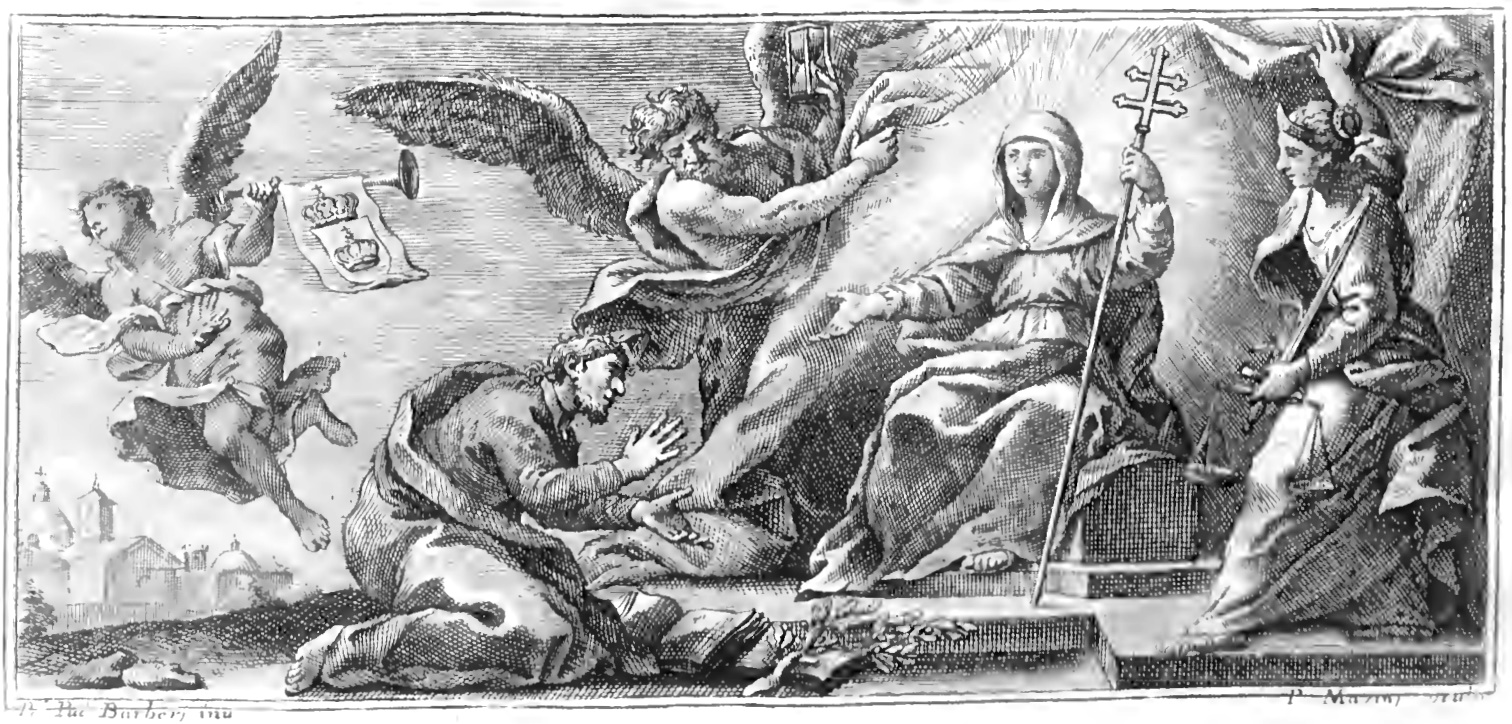
\includegraphics[width=7in]{Picture7.jpg}\end{center}}

\predate{\vspace{-1em} \begin{center} \LARGE \bfseries \underline{\underline{\color{Red}MATRITI ANNO MDCCLXXV.}}\\ \vspace{+.5em}}
\date{\color{black} \large \mdseries \underline{{\Large A}pud \normalsize {\Large J}OACHIMUM {\Large I}BARRA {\Large S.C.R.M. \& Dignit. Archiep. Typog.}}\\ \vspace{+.5em}}
\postdate{\color{Red} \itshape \bfseries REGIO PERMISSU.\end{center}}

\begin{document}

%pp6 placeholder

%pp7
% \title{\bfseries {\zallmancaps \Huge \color{Red} B R E V I A R I U M} \\ \huge G O T H I C U M \\ \LARGE {\mdseries \itshape \color{Red} S E C U N D U M \ \ R E G U L A M} \\ \Huge BEATISSIMI ISIDORI \\ \large \mdseries {\itshape \color{Red} A R C H I E P I S C O P I \ \ H I S P A  L E N S I S} \\ \small {\large J}USSU {\large C}ARDINALIS {\large F}RANCISCI {\large X}IMENII DE {\large C}ISNEROS PRIUS EDITUM; \\ {\color{Red} \itshape N U N C \ \ O P E R A} \\ \large EXC.\textsuperscript{MI} D. FRANCISCI ANTONII LORENZANA \\ \normalsize \itshape {\color{Red} SANCT\AE \ ECCLESI\AE \ TOLETAN\AE \ HISPANIARUM PRIMATIS} \\ {\color{Red} Archiepiscopi recognitum} \\ \upshape AD USUM SACELLI MOZARABUM.}

\newgeometry{margin=.5in}
\maketitle
\bookmark[startatroot,dest=page.1]{TITLUM}

%pp8
\newpage
\thispagestyle{empty}
\setcounter{page}{0}
\mbox{}
\newpage

\frontmatter

%pp9
\restoregeometry
% \setcounter{page}{1}
\pagenumbering{Roman}
\thispagestyle{fancy}
\fancyhead{}
\fancyfoot{}
\renewcommand{\headrulewidth}{0pt}
\setlength{\headheight}{16pt}
\setlength{\headsep}{6pt}
\fancyhead[C]{(\thepage)}

\begin{center} \hypertarget{Preface} \Large
FRANCISCUS ANTONIUS LORENZANA
\end{center}

\begin{center} \large \itshape
ARCHIEPISCOPUS TOLETANUS HISPANIARUM PRIMAS
\end{center}
\centerline{\Large LECTORI SALUTEM.}
\bookmark[dest=Preface]{LECTORI SALUTEM}
\vspace{+1em}

\lettrine[lines=2]{A}{B} hujus\rightmarginnote{Utilitas editionis\\Gothici Ritus.} nostri Pastoralis muneris exordio nihil altius fuit animo insitum, quam majorum sequi vestigia, pr\ae cipue clarissimi Cardinalis Francisci Ximenii de Cisneros, qui pene obliteratum Gothicum, seu Mozarabicum Ritum typis mandavit: ut posteris Gothorum Patrum memoria rediret, \& quasi revivisceret honos debitus Osio, Leandro, Fulgentio, Isidoro, Braulioni, Eugenio, Helladio, Juliano, Ildephonso, \& aliis Patribus de nostra Hesperia optime meritis, strenuis fidei athletis, Ecclesiarum Hispani\ae \ columnis, Gothic\ae \ gentis decori, \& Pr\ae sidibus Conciliorum.
\par Huic operi obnixe incumbentes pr\ae \ oculis habuimus, propriisque manibus pervolvimus pervetustos Gothicos Codices veterem liturgiam redolentes, octingentis abhinc ferme annis manu exaratos, quingentis ad minus ante triste natale Lutheri, Calvini, Sectariorum, \& Novatorum adversus Sacramenta, queis Sancta Mater Ecclesia mirabiliter fovetur, \& nutritur, ut fidei hostes ad meliorem frugem convertantur, vel saltem Sacra Mysteria in tam perantiquis autographis perlegentes, obmutescant.
\par Ecclesia\rightmarginnote{Sedes Apostolica\\unitatem Ritus\\exoptat, sed diversi-\\tatem huad omnino\\damnat.} Romana omnium Mater, \& Magistra summopere insudavit, ut sacra liturgia per universam orbrem eodem Ritu celebraretur; \& sic una esset omnium fidelium oratio: verumtamen Missalia, \& Breviaria antiqua non abolevit; imo tamquam in Sacrario Psalterium secundum veterem versionem Italam ab Augustino, \& aliis Patribus pr\ae laudatum retinet; in Vaticana Capella pr\ae cinit, ejusque Codices in Bibiliotheca tamquam in serinio pectoris recondit.
\par Ipsummet\rightmarginnote{Resplendens in qui-\\busdam approbatis\\Ritibus pulchra varie-\\tas Ecclesiam mirifice\\ornat.} Sacrum Concil. Trid. maximam inde utilitatem provenire agnoscens, statuit: Religiosos Ordines ducentis ante ipsum annis peculiari Ritu utentes, eum retinere posse, tam in Sacrificio Miss\ae , quam in divino Officio persolvendo.
Ob id longissima temporis pr\ae scriptione, \& immemorabili consuetudine suffulti Cistercienses, Carthusiani, Eremit\ae \ Calceati Montis Carmeli, \& Pr\ae dicatores Ordinis S. Dominici proprios Ritus \& C\ae remonias observant; ut insimul hoc modo in Ecclesia Dei unitas Sacrificii resplendeat; \& veteri Ritu Romano cum politiori collato Sponsa Chrsiti mirabili circumdetur varietate.
\par Zelo\rightmarginnote{Laudatur studium\\Cardinalis Ximenii de\\Cisneros in Missalis \&\\Breviarii Muzarabici\\editione.} fidei accensus eximus ille Cardinalis Ximenius, Christianus, \& Politicus Heros sparsos undique Gothicos, Isidorianos, seu Muzarabicos Codices in unum collegit; viros doctissimos undequaque
%pp10
accivit: peritiores in Muzarabico Ritu Sacerdotes selegit; iisque divitiis onustus, Breviarium secundum regulam S. Isidori tandem anno 1502 pr\ae lo commisit.
\par Verum ne metas recti ordinis transgrediamur, primo de Etymologia hujus Sancti Officii, postea de rebus ad ejus antiquitatem spectantibus agemus.
\par Etymon\rightmarginnote{Etymon Ritus\\Muzarabici, Gothici,\\Isidoriani, \& Toletani.} igitur Muzarabici Officii usurpatur secundum denominationes Nationum, inter quas Hispani victitabant.
Revera namque ordine chronologico Ritus licet sit secundum temporum vicissitudine, \& Pr\ae latorum ordinationes variatus, primo denominari debet {\itshape Romanus}, \& {\itshape Hispanicus}, traditione descendens a Sanctorum Petri, \& Pauli Discipulis primis Ecclesi\ae \ Hispani\ae \ fundatoribus, \& Pr\ae sulibus, scilicet Torquato, Ctesiphonte, Indaletio, Hesychio, Euphrasio, Secundo, \& C\ae cilio, qui ad Hesperi\ae \ nostr\ae \ oras pervenientes, eam fidei lumine illustrarunt; deinde {\itshape Gothicus}, post Reccaredi Gothorum Regis ad Catholicam fidem conversionem, publicamque in Concil. III. Tolet. Arian\ae \ H\ae reseos abjurationem.
\par Cum\rightmarginnote{Ordinatores, \& Cor-\\rectores Gothici\\Ritus S. Isidorus,} Leander, \& ejus frater Isidorus multa in sacra Liturgia, \& Officio depravata, corrupta, \& Arianorum perfidia inversa comperissent (incredibile namque est, a tempore Athaulfi usque ad Reccaredum vigentibus Arianis erroribus, exulibus Episcopis Catholicis, plurima in sacra autographa non irrepsisse vitia), ea\leftmarginnote{\begin{flushright}\& Leander; pr\ae cipue\\ vero Concil. IV.\\Toletan. normam\\in Divinis Officiis\\pr\ae scripsit.\end{flushright}} a mendis expurgare, puriora reddere, \& in meliorem ordinem redigere cogitarunt; cujus causa Leander, \& Isidorus de divinis Officiis scripserunt, \& totus fere scopus Concil. IV. Tolet. pr\ae side S. Isidoro, fuit, ordinem in Sacrificio Miss\ae , \& in divinis Officiis stabilire, per universam Hispaniam, \& Galliam extendere, deturpatamque faciem ad pristinum statum restituere.
\par Ob\leftmarginnote{\begin{flushright}Isidorus Vicarius\\Apostolicus; \&\\Ritus Isidorianus\\nuncapatus.\end{flushright}} tantos exantlatos labores, \& diuturnas elucubrationes S. Isidori c\oe pit merito Ritus nuncupari, {\itshape Isidorianus: Breviarium, \& Officium, secundum regulam Beatissimi Isidori}; hoc est, secundum Canones Concil. IV. Tolet. ab ipso pr\ae cipue elaboratos, utpote Pr\ae side Concilii, \& Sedis Apostolic\ae \ Vicario, Ritus \& disciplin\ae \ Ecclesiastic\ae \ Moderatore, \& totius Orbis fulgentissimo sidere.
\par Postquam\leftmarginnote{\begin{flushright}Ritus dictus\\Muzarabicus.\end{flushright}} misere a Mauris Hispania nostra fuit occupata, Christianique Arabibus victu, vestitu, \& pluries connubio mixti, inito pacis f\oe dere, a Maurorum Regibus quasdam obtinuerunt Ecclesias; suis Catholicis Ritibus retentis, Missale, \& Officium {\itshape Muzarabica} fuere appellata.
\par Quis\leftmarginnote{\begin{flushright}Christiani tempore\\Mahumetic\ae \ Domi-\\nationis Catholicam\\Ritum retinent.\end{flushright}} vel lippis oculis non videt, per quadringentos ferme annos Arabici dominii in Toletana Civitate occulte Sacra a Christianis multoties sine Pr\ae sule, \& sine Episcopo fieri?
Quis non miratur hunc Ritum hac tempestate penitus non deperiisse Regii Sacerdotii deficiente virtute? \& si aliquoties furtim, secreto, aut magno
%pp11
pretio Saracenis a Christicolis persoluto, Episcopus hujus Sedis Toletan\ae \ eligebatur; nec, scholis clausis, peritiorem, nec sanctiorem, amissa libertate invenire licebat, interdicto pr\ae dicandi \& docendi munere, \& barbarie cunctos obnubilante.
\par Affulsit\leftmarginnote{\begin{flushright}Ritus Gothicus\\c\oe pit nuncapari\\Toletanus.\end{flushright}} tandem optata dies, qua inclytus Alphonsus Sextus Toletum expugnavit, suamque in potestatem redegit: A Sacris exorsus: Mezquita olim, Sacra Basilica effecta est; e Gallia doctissimos, \& religiosissimos viros evocavit, ut ad Episcopales Cathedras eveheret; Cluniacenses Monachos tum maxime florentes, ad Canonicatus, \& dignitates Ecclesi\ae \ Toletan\ae \ adduxit; Bernardum Toleti Pr\ae sulem constituit; Sanctum Petrum Oxom\ae ; alium Bernardum Segonti\ae ; \& Sanctum Geraldum Brachar\ae .
Hoc ex tempore Mozarabicum Officium nominatum fuit {\itshape Toletanum}; quia Toleti commorari Castell\ae , \& Legionis Reges, magnificareque Urbem, \& Ecclesiam c\oe perunt: ob loci securitatem, munitiorem, \& faciliorem accessum ad c\ae tera expugnanda oppida a Mauris occupata; \& exinde Urbs parva munita loco, Regia civitas nuncupabatur.
\par A\leftmarginnote{\begin{flushright}Memoria Card.\\Mendoza com-\\mendatur.\end{flushright}} tempore Alphonsi Sexti usque ad Catholicos Reges Ferdinandum, \& Elisabetham cum frui quiete ac pace Castell\ae \ Reges non potuerint, hinc inde discurrebant: bello assueti, de expellendis Mauris ab universa Hispania sedulo cogitabant: tenebras ignoranti\ae \ fas non erat penitus discutere; quousque Granatensi civitate expugnata, Catholici Reges in melius res ordinare suis egregiis Consiliariis magnis Cardinalibus Petro Gonzalez de Mendoza (eoque vita functo) Francisco Ximenio de Cisneros commendarunt.
Ista clarissima Ecclesi\ae \ lumina, Universitates, Collegia, Xenodochia, Orphanotrofia, Cathedrales, \& Collegiatas Ecclesias erigi in Hispania, \& in Indiis curarunt; \& qu\ae dam pia egregia monumenta suis sumptibus posteris imitanda reliquere.
\par Cardinalis\leftmarginnote{\begin{flushright}Missale \& Officium\\Isidorianum Card. Xi-\\menius edere intendit.\end{flushright}} Ximenius quasi apis argumentosa cito selegit Biblia Sacra, Missale, \& Officium Isidoriana, ut quantocius pr\ae lo, nuper in Hispania introducto, committerentur; nihil enim utilius, gratius, \& Religioni commodius judicavit, quam sacros libros vegetiores, \& puriores omnibus f\oe nerari.
\par In\leftmarginnote{\begin{flushright}Finis Card. Ximenii\\in editione Muza-\\rabici Ritus.\end{flushright}} Editione Missalis, \& Breviarii {\itshape Isidoriani} nullatenus intendit pr\ae clarissimus hic vir aliquid detrahere auctoritati veteris {\itshape Romani}, quin potius extollere.
Collata etenim hujus correctione cum antiquo Gothico, evidenter demonstratur, Ecclesiam Sponsam Christi semper, \& ubique unam fuisse; eodemque Spiritu coadunatam, inconsutilem, non ab H\ae reticis dilaceratam, divisam in partes, sortitam, \& a summo usque deorsum ab illis scissam.
Licet non idem modus, ordo, \& latini sermonis facundia in omnibus precibus appareat; in Gothicis tamen exemplaribus ingenuus sermo resplendet, non arte politus, sed vetustatem redolens, ob idque Grammatices regulis non
%pp12
tam arcte astrictus, ut in uno vel altero loco hujus nostr\ae \ editionis videre licet; c\ae terum propter CC. venerabilem canitiem ea ill\ae sa reliquimus; \& ob levamen legentium, maxime recitantium, unamquamque dictionum suo proprio accentu insignivimus: in Missali autem, \& Breviario Romano cuncta recte satis disposita, perpolita, a pluribus mendis purgata, \& vigiliis clarissimorum Cardinalium Baronii, Bellarmini, \& aliorum in melius redacta: Hymni etenim S. Ambrosii, \& aliorum Patrum ad meliorem concentum, \& mensuram versus fuerunt reducti: suis quique locis aptati; ita ut \& sensum retinerent, \& ab Oratoribus, \& Poetis Latinis non deviarent.
Hucusque de Nomenclaturis hujus Sancti Officii.
\par Inter\rightmarginnote{Versione antiqua Itala\\utuntur Muzarabici\\Sacerdotes.} res ad antiquitatem Liturgi\ae \ Gothico-Hispanic\ae \ spectantes, Versio primum locum vindicat sibi.
Tanti enim habita fuit apud Veteres, \& Neotericos versio vetus Itala, ut de ea S. Augustinus asserere non dubitaverit in interpretationibus c\ae teris pr\ae ferendam, {\itshape nam est verborum tenacior cum perspicuitate sententi\ae }: hacque pr\ae cipue utuntur Mozarabici Sacerdotes.
\par Hic\rightmarginnote{Opera Ortizii in\\editione Breviarii.} scitu dignum est, quod ne antiqui Ritus Gothico-Hispani deperiret memoria, editionem Breviarii commisit pr\ae laudatus Ximenius Doctori Alphonso Ortizio, Canonico Toletano, qui in Dedicatione operis fatetur: {\itshape Officia nocturna pariterque diurna} in lucem edita {\itshape dignitate} quidem egregia, {\itshape cognitione, \& castigatione fuisse difficilia; diu multumque operoso studio recognita: antea namque pene omnia in libris veteribus confusa, atque incognita penes eruditos jacuisse; impensis vero, \& Cardinalis opera suis locis qu\ae que reposita, characteribus, atque periodis distincta, verbis, \& sententiis dilucidata; ac diu senio periclitata Officia Isidoriana, annositate deleta, futuris s\ae culis sine difficultate jam perlegenda.}
\par Hanc\rightmarginnote{Auctores: qui Codices\\Gothicos Sacri Ritus\\ediderunt.} provinciam edendi Sacros Codices postea aggressi sunt Flaminius Nobilius, Morinus, Joannes Martian\ae us, Thomas Hetarneus, Faber Stapulensis, Josephus Maria Caro, Cardinalis Thomasius, \& Petrus Sabatier alios recensens, \& merito Blanchinium extollens: ex his duobus postremis clarissimis Auctoribus quidquid reperuimus ad nostram Breviarii Gothici Editionem perutile, delibavimus, non vultu Ritus immutato, sed tantum correcto, collatis lectionibus cum Vaticanis CC. Veronensibus, Corbejensibus, Parisiensibus, S. Germani, \& aliis.
\par In tantum deserviit editio Versionis veteris Ital\ae \ a Petro Sabatier magno labore facta, ut ea duce non c\oe cutiremus, nec c\ae spitaremus; nam nec verbum fere in nostro Psalterio invenimus exaratum, quod in alio ex M. SS. pr\ae cipue in Bibliis Gothicis Toletanis, \& in D. Augustino non legatur: hoc modo tuta nobis patuit via ad nostri Breviarii correctionem quando vel mendum Typographi apparebat apertum, vel si etiam h\ae sitare de sensu alicujus vocis contingebat, aliis veteribus lectionibus concordantibus firmabamur.
%pp13
\par Mirabilis\rightmarginnote{Mirabilis in Mss. Cod.\\substantialis unitas.} multiformis gratia Dei!
Mirabilis Spiritus Paraclitus septiformis munere, \& multiformis dono linguarum, qui dignatus est ex visceribus sacri textus absque substantiali sententi\ae \ mutatione tot Versiones ab Ecclesia non rejectas; totque generibus linguarum depositum fidei in M. SS. Gothicis Vaticani, Hispani\ae , \& Galliarum nobis in hunc diem sartum tectum servare!
\par Ne\rightmarginnote{Vulgata editio c\ae teris\\pr\ae ferenda; ali\ae \\non contemnend\ae ,\\ \& vetus Itala maxime\\habenda.} vero vagandi licentia fidelibus indiscriminatim tribueretur, \& simul H\ae reticorum libertas coerceretur, Sacrum Concilium Tridentinum privatis arbitrium judicii in sacris discernendis ademit; \& ex omnibus versionibus, \& editionibus Sacrorum Bibliorum Vulgatam selegit: c\ae teris pr\ae tulit, \& authenticam declaravit; ne in re tam gravi Laici, \& Femin\ae \ Judices constituerentur.
Non vero alias quasdam Versiones parvipendit, Italicam pr\ae cipue; immo ut hujus innotesceret antiquitas, \& veritas, in officio Romano ad Matutinum Psalmus, seu Invitatorium {\itshape Venite exultemus Domino} juxta veterem versionem Italam ferme adamussim recitatur, retenta solum in die Epiphani\ae \ Domini Vulgata; \& Gregorius Magnus utraque translatione nunc Nova, nunc Vetere, utebatur.
\par In\rightmarginnote{In Missali, \& Brevia-\\rio Romano qu\ae dam\\inveniuntur juxta} Introitu Missarum videsis Gradualia, \& Tractus ipsiusmet Missalis Romani. Passim inveniuntur versiculi secundum veterem Italam versionem, qua utitur Psalterium Gothico-Hispanum: exempli causa: In Introitu Dominic\ae \ Septuagesim\ae \ recitantur illa verba {\itshape Circumdederunt me gemitus mortis}; \& non\leftmarginnote{\begin{flushright}versionem Italam\\veterem.\end{flushright}} {\itshape doloris} juxta Vulgatam; in Communi Martyrum tempore Paschali Psalm. 134. {\itshape in servis suis consolabitur}, juxta Vulgatam {\itshape deprecabitur}.
\par Ne\leftmarginnote{\begin{flushright}Psalterium Isidori-\\anum lectioni S.\\Augustini ut in\\plurimum congruit.\end{flushright}} videamur Psalterii Isidoriani Versionem nimium extollere, \& pro nostro arbitrio asserere, veteri Italic\ae \ quam summopere ut dictum est, Augustinus commendat, eam esse simillimam, qu\ae dam loca proferemus.
In psalmo 47. legitur in Vulgata {\itshape odientes}, \& in Psalterio Isidoriano {\itshape odio habentes}, eodem modo quo S. Augustinus legit: Psalmo 18. v.3. tam in Vulgata, quam aliis versionibus {\itshape eructat}, in versione vero veteri Itala legitur {\itshape eructuat}, ut etiam in Augustino; insuper vers. ejusdem Psalmi Vulgata: {\itshape Si mei non fuerint dominati}; Psalterium Isidorianum {\itshape dominata}, sicuti Augustinus: Psalmo 20. vers. 3. {\itshape desiderium cordis} legitur in Vulgata, \& aliis quibusdam versionibus; in Psalterio vero Mozarabico {\itshape anim\ae }, ut in Augustino; \& Ecclesia Romana in Communi unius Martyris pluries repetit {\itshape anim\ae }.
\par Juxta Vulgatam centum quinquaginta Psalmi Davidis, seu ejus Discipulorum enumerantur; tamen in nostro Psalterio Isidoriano, \& in Versione veteri Italica superadditur Psalmus 151, cujus initium: {\itshape Pusillus eram inter fratres meos, \& adolescentior in domo patris mei} \&c. cum hac epigraphe: {\itshape Hic Psalmus proprie scriptus in David extra numerum, cum pugnator esset adversus Goliam solus}: \& si conferas non epigraphem sed Psalmi verba, absdubio in Versione veteri Italica
%pp14
(nusquam in editione Vulgata, \& aliis) eadem reperies.
\par Pr\ae terea sedulo scrutare Psalmum 118 {\itshape Beati immaculati in via}, \& tot antiquitatis notas, tot annotationis numeros H\ae braicis, Romanis, \& antiquis Hispanicis litteris descriptos reperies, ut nulla remaneat dubitatio.
Incipit a littera H\ae braica {\itshape Aleph}, sequitur numerus Romanus I, alius Hispanicus adjicitur, omnesque idem significant, scilicet numerum primum: postea indigitatur initium mystic\ae \ significationis, \& sic deinceps totus Psalmus per octo versiculos successive in capita distribuitur: in versione Vulgata tantum litter\ae \ H\ae braic\ae \ apponuntur, \& illa alia in nostro Psalterio addita antiquitatem redolent.
Psalmo 95. v. 8. h\ae c verba in nostro Codice leguntur: {\itshape Dicite in Nationibus: Dominus regnavit a ligno}, a Justino, Tertuliano, atque aliis Patribus tantopere commendata, \& a Fortunato in hymno, {\itshape Vexilla Regis prodeunt}, hoc modo intexta: {\itshape Impleta sunt, qu\ae \ concinit David fideli carmine, dicens in Nationibus: Regnavit a ligno Deus}; \& tamen in Vulgata non reperiuntur, ut in veteri Itala, \& Psalterio nostro.
\par Scire hic cupiet eruditus Lector, a quo, \& quo s\ae culo hoc Psalterium M.S. sit exaratum? \& ut ob elucidationem rei utriusque fines recti judicii non pr\ae tergrediamur, asserimus: Codicem tria continere, scilicet, Psalterium, Cantica, \& Hymnos; c\ae terum in Pr\ae locutione Acrostica Hymnorum leguntur initio cujusque exametri litter\ae , ex quibus prodeunt h\ae c verba: {\itshape Mauricus obtante Veraniano edidyt}, ex quibus conspicuum apparet, Exscriptorem fuisse quemdam Mauricum Veraniani votis, aut jussu: tamque jubentis, quam exequentis Nos latet notitia; nec conjecturis locus est, cum nulla in Conciliis Toletanis Episcopi Veraniani mentio fiat: nam licet Mauritius Oretanus Episcopus, \& Vera Tarraconensis Toletanis Conciliis subscripserint; tamen nullum ex hoc fundamentum elici potest; \& tantummodo ad scriptur\ae \ signa recurrere licet.
\par In Canticis superscriptio Prophetarum inversa tibi videbitur; nam Jeremias pro Nehemia, Zacharias pro Azaria, Jeremias pro Mich\ae a, Isaias pro Jeremia, \& Osea: hoc partim Exscriptoris culpa, partim aliis de causis contingere potuit; \& ne supercilium extollas, illico tibi exemplum simile in nostra Vulgata occurrit; nam cap. 27. Matth. vers. 9, h\ae c verba: {\itshape Acceperunt triginta argenteos pretium appretiati}, \&c. relata sunt tamquam dicta a Jeremia Propheta illis verbis: {\itshape Tunc impletum est, quod dictum est per Jeremiam}; quando certo constat non a Jeremia, sed a Zacharia esse prolata.
Ulterius cap. 1. Marci v. 2. apponuntur illa verba: {\itshape Ecce ego mitto Angelum meum ante faciem tuam; juxta Isaiam prophetam}, \& revera sunt Malachi\ae .
Ad has, \& alias difficultates enodandas in varias Expositores abeunt sententias; sed ad nostrum institutum magis arridet S. Hieronymus lib. 2. in Amos cap. 5. hisce verbis: {\itshape In omnibus Scripturis sanctis observandum est Apostolos, \& Apostolicos Viros in ponendis testimoniis de Veteri Testamento non verba considerare, sed sensum.}
%pp15
\par Ex\rightmarginnote{Multa in Missali Romano\\ex versione veteri\\Itala deprompta esse\\Clemens VIII. testatur.} his colligitur: Hispanicam Ecclesiam in Sacrorum Bibliorum Versione in plurimis adh\ae rere veteri Italic\ae , cujus mentionem S. Augustinus facit; \& in Missali, \& Breviario Romano juxta eamdem, \& non alias tunc temporis vigentes, plures appositos fuisse versiculos Clemens VIII. in bulla Romano Missali pr\ae fixa sequentibus verbis testatur: {\itshape Qui} (Pius V) {\itshape \& si multis propositis p\oe nis severissime caverit, ne illi vel adderetur, vel ulla ratione demeretur; tamen progressu temporis sive Typographorum, sive aliorum temeritas, \& audacia effecit, ut multi in ea qu\ae \ his proximis annis excusa sunt Missalia, errores irrepserint, quibus vetustissima illa sacrorum Bibliorum Versio, qu\ae \ etiam ante S. Hieronymi tempora celebris habita est in Ecclesia, \& ex qua omnes fere Missarum Introitus, \& qu\ae \ dicuntur Ggradualia, \& Offertoria accepta sunt, omnino sublata est ... cujus rei pr\ae textus fuisse videtur, ut omnia ad pr\ae scriptum sacrorum Bibliorum Vulgat\ae \ editionis revocarentur.}
\par Licet enim Hieronymus in Sacris Scripturis exponendis Doctor Maximus censeri debeat; tamen in Ecclesia Latina magni ponderis semper habita est auctoritas Augustini.
Nec eruditos latet, Hispanicam Ecclesiam ejus opera pr\ae \ oculis habuisse, cum ob propinquitatem regionum, tum ob Epistolarum frequentiam, \& Episcoporum Africanorum cum Hispanicis communicationem.
\par Canticum\rightmarginnote{Probatur ex Cantici 23.\\Auctoris Appellatione.} XXIII. in nostro Psalterio canticum {\itshape Tobi} inscribitur, non {\itshape Tobi\ae }; \& eodem modo S. Augustinus, qui semper seniorem {\itshape Tobim}, juniorem {\itshape Tobiam} appellat.
\par S.\rightmarginnote{S. Leander a S. Gregorio\\Magno commendatur.} Leander apprime charus fuit, \& amicitia conjunctissimus S. Gregorio Magno, necnon S. Isidorus; ejus rei evidens argumentum est quod Commentaria in Job papa Gregorius Leandro dicavit, eum alloquens verbis amore \& reverentia plenis.
Quis igitur san\ae \ mentis hos Sanctos Doctores ejusdem instituti mutuo inter se non contulisse consilia, versiones sacras, \& libros, quibus fides Catholica fulciretur, \& Gothorum gens nuper ad fidem conversa in ea stabiliretur, opinabitur?
Adducat alius simile Dedicationis exemplum Summi Pontificis, magnique Ecclesi\ae \ Doctoris: in medium afferat alia verba tant\ae \ benevolenti\ae \ plena sicut illa Gregorii ad Leandrum ex regist. lib. 4. epist. 46. {\itshape Quanto ardore videre te sitiam, quia valde me diligis, in tui tabulis cordis leges; sed quia longo terrarum spatio disjunctum te videre nequeo, unum, quod mihi de te dictavit charitas, feci; ut regul\ae \ Pastoralis librum, quem in Episcopatus mei exordio scripsi, \& libros, quos in expositionem B. Job jam dudum me fecisse cognovisti, Sanctitati Tu\ae , communi filio Probino Presbytero veniente, transmitterem.}
Et in fine Epistol\ae \ de brevitate sese excusans h\ae c verba auro cedroque digna eumdem alloquens subjungit: {\itshape Ipsa charitati tu\ae \ Epistol\ae \ me\ae \ brevitas innotescit, quando ei parum loquor, quem magis omnibus diligo.} Inter quos, qu\ae so, Ecclesi\ae \ Patres strictius
%pp16
amiciti\ae \ vinculum usquam perlectum est?
\par Isidorus,\rightmarginnote{S. Isidorus S. Gregorio\\Magno acceptissimus\\fuit, \& a Leone IV.\\commendatus.} etsi non discipulus, eidem Summo Pontifici commendatissimus fuit, qui non solum auctoritate Apostolica ejus electionem confirmavit, \& electum sacro Pallio decoravit; sed etiam ejus in universa Hispania Vicarium constituit.
Non minorem Leo IV. de eo opinionem concepit, qui ad Britanni\ae \ Episcopos scribens, asserit: {\itshape Isidori dicta, sicut Hieronymi, \& Augustini retinenda esse ubi inusitatum contigerit negotium, quod per Canones minime definiri possit.}
Ejus fama eo tandem excrevit, ut vix ab ejus obitu decem \& sex annis elapsis, Toletana Synodo duorum supra quinquaginta Episcoporum plaudente, ipsoque S. Ildephonso suffragante, {\itshape Doctor egregius, Catholic\ae \ Ecclesi\ae \ novissimum decus, in s\ae culorum fine doctissimus, \& cum reverentia nominandus} appellari meruerit.
\par Perfacili negotio ex hucusque dictis autumare quis poterit, quot flores ex Ecclesia Romana, ejusque Ritu hi Sacri Doctores decerpserint, cum via illis ad Procuratores mittendos patebat; \& iisdem in prosperis bene agendis Summi Pontifices maxime favebant.
\par Jam\rightmarginnote{Eadem versio, quam S.\\Gregorius Veterem vul-} non demiror, Psalterium juxta versionem veterem Italam, qua Hispaniarum Patres utebantur, in Summi Pontificis sacello, nec non Venetiis in majori Ecclesia S. Marci in hodiernum diem recitari: eodem\leftmarginnote{\begin{flushright}gatam seu Translationem\\appellat, cum ea conven-\\it, quam nos veterem\\Italam nuncupamus.\end{flushright}} enim spiritu Patres Hispanici agebantur, eadem Apostolica disciplina dirigebantur, \& a S. Petri Sede, quod illis deerat, mutuabantur; eademque versio quam S. Gregorius veterem Vulgatam, seu translationem appellat, a S. Augustino Itala nuncupatur.
\par Hactenus de Versione hujus Sancti Officii. Nunc vero antiquitatem Liturgi\ae \ Gothico-Hispanic\ae \ patefaciam, primo ex vetustate Codicum, secundo ex institutoribus, seu compilatoribus ejus, demumque ex Notis Cantus appellati Eugeniani textui appositis.
% !!!!!!!!!!!!!!!!!!!!!!!!!!!!!!!!!!!!!!!!!!!!!!!!!!!!!!!!!!!!!!!!!!!!!!!!!!!!!!
% !!!!!!!!!!!!!!!!!!!!!!!!!!!!!!!!!!!!!!!!!!!!!!!!!!!!!!!!!!!!!!!!!!!!!!!!!!!!!!
% !!!!!!!!!!!!!!!!!!!!!!!!!!!!!!!!!!!!!!!!!!!!!!!!!!!!!!!!!!!!!!!!!!!!!!!!!!!!!!
% !!!!!!!!!!!!!!!!!!!!!!!!!!!!!!!!!!!!!!!!!!!!!!!!!!!!!!!!!!!!!!!!!!!!!!!!!!!!!!
% !!!!!!!!!!!!!!!!!!!!!!!!!!!!!!!!!!!!!!!!!!!!!!!!!!!!!!!!!!!!!!!!!!!!!!!!!!!!!!
% !!!!!!!!!!!!!!!!!!!!!!!!!!!!!!!!!!!!!!!!!!!!!!!!!!!!!!!!!!!!!!!!!!!!!!!!!!!!!!
% !!!!!!!!!!!!!!!!!!!!!!!!!!!!!!!!!!!!!!!!!!!!!!!!!!!!!!!!!!!!!!!!!!!!!!!!!!!!!!
% !!!!!!!!!!!!!!!!!!!!!!!!!!!!!!!!!!!!!!!!!!!!!!!!!!!!!!!!!!!!!!!!!!!!!!!!!!!!!!
% !!!!!!!!!!!!!!!!!!!!!!!!!!!!!!!!!!!!!!!!!!!!!!!!!!!!!!!!!!!!!!!!!!!!!!!!!!!!!!
% !!!!!!!!!!!!!!!!!!!!!!!!!!!!!!!!!!!!!!!!!!!!!!!!!!!!!!!!!!!!!!!!!!!!!!!!!!!!!!
% !!!!!!!!!!!!!!!!!!!!!!!!!!!!!!!!!!!!!!!!!!!!!!!!!!!!!!!!!!!!!!!!!!!!!!!!!!!!!!
% !!!!!!!!!!!!!!!!!!!!!!!!!!!!!!!!!!!!!!!!!!!!!!!!!!!!!!!!!!!!!!!!!!!!!!!!!!!!!!
\par Miseranda deflendaque Hispaniarum vastatio a Saracenis facta, Hispanorum Patrum memoriam non abolevit; quamvis plurima eorum scripta, partim abrasa, partim mendis et fabulis conferta, partim deperdita, spurcata partim, et denique igni tradita, penitus oblivioni dare intenderint pagani, postliminio tamen, Mauris expulsis, opera et studio cardinalium Ximenii, Loaisae et Aguirrii, in Editione ritus et concil. Toletanorum honos tantis Patribus est restitutus.

Si aliquod in mss. Codices mendum irrepsit, exscriptorum, non auctorum vitio est vertendum; si enim hodie cum ars typographica viget, passim in libris errores inveniuntur et menda, quid mirum si inventionis initio Missale et Breviarium Isidorianum mendis scateret quam plurimis? Nec tantum de labore nostro confidimus, ut fatum simile aliqua in parte non nobis contingat; pag. enim 59 invenitur sancti Thomae Cantuariensis nomen, prout exstat in Editione D. Ortizii: appositum illic aut potius elapsum est praeter mentem nostram.

Gothici Codices, quos evolvimus, senio confecti, disrupti, lacerati, characteribus fere oblitteratis et absumptis, blattas non pascunt, saepe enim prae manibus habentur; sed tinea et aerugo non solum membranas, papyra, ligna, etiam marmora corrodunt et demoliuntur.

Plures regnicolae et exteri auctores absque ulla haesitatione testantur Compluti autographa Gothica manuscripta, quae ad excudendum Missale et Breviarium Isidorianum deservierunt, asservari. Haec, dum essemus in praefata civitate, sedulo et avidissime quaesivimus; sed incassum exspectavimus: nec, juxta magistrum Florezium, adesse poterant; nam Toleti excusa fuerunt Missale et Breviarium, inibique propterea autographa asservari oportebat. Mœrentes, utpote tali desiderio fraudati, Bibliothecam nostrae sanctae Ecclesiae Toletanae repetiimus, ubi vota nostra aliquatenus adimplevimus.

In ea octo Codices Gothici mss. reperiuntur, quorum in uno praeter septem missas a sancto Ildephonso, ut creditur, cum cantus notis compositas, continentur officia Nativitatis, Circumcisionis et Apparitionis Domini, Assumptionis beatae Mariae, et officium Joannis apostoli et evangelistae; in alio officium integrum Quadragesimae usque ad Dominicam Palmarum exclusive; in altero, praeter nonnullas missas, officium hebdomadae majoris usque ad Pascha inclusive, et aliqua sanctorum officia; in alio officia sanctorum per annum; in alio Epistolae et Evangelia per annum; in alio missae sanctorum per annum; in alio denique integrum Psalterium cum canticis et hymnis. Praeter nos Codices asservantur in praefata bibliotheca Gothica Biblia, quae tempore Mahumeticae captivitatis fuerunt propria Servandi, episcopi Astigitani; postea Joannis, episcopi Carthaginensis et Cordubensis, qui ea donavit Ecclesiae Hispalensi, aera 1026, anno Christi 988.

Tamen non fuco depingere faciem hujus pervetusti Codicis in animo est, nec velare quod perspicacissimis eruditorum oculis patefiet. Aliquod, licet leve, in quorumdam verborum transmutatione discrimen inter Breviarium Isidorianum prelo datum a cardinali Ximenio, et inter memoratos Codices Mss. agnoscimus; quapropter conjicere licebit, vel Alphonsum Ortizium, canonicum Toletanum, alia prae oculis habuisse autographa, nunc temporis deperdita; vel ipsummet Alphonsum, cardinalis Ximenii auctoritate munitum, in locis obscuris Psalmorum, ubi anxietate premebatur, ad Vulgatam, seu aliam, recurrisse versionem, et juxta eam quaedam verba addidisse.

Verum tam in hoc ipso, quam in festivitatibus et sanctis officio Mozarabico adjectis, ansam impugnatoribus praestitit; quia cum luce meridiana clarius sit festum Corporis Christi post Berengarii errores compositum; sanctos Thomam Cantuariensem, Franciscum, et alios, quorum in Breviario Mozarabico per annum memoria fit, multis saeculis post sanctum Isidorum Hispalensem floruisse; inde ad derogandum auctoritati Breviarii occasionem arripiunt; sed injustissime, ut pluribus rationibus comprobat et evincit praefatus R. P. Henricus Florezius.

Missale et Breviarium Romanum a summis pontificibus Pio V, Clemente VIII et Urbano VIII correctum, non desiit esse Romanum, ex vetustissimis exemplaribus deductum, et apostolorum traditione descendens, ex additione quarumdam festivitatum, quae primis saeculis non celebrabantur, vel sanctorum nostro praesenti saeculo, vel proxime praecedentibus beatorum albo ascriptorum, de quibus missa et officium proprium recitantur. Ne fas cuiquam conjicere antiquitatem minui propter tale incrementum Ecclesiae et majorem ritus extensionem.

 Pari modo Missale et Breviarium Hispanicum talem denominationem non amisit post gentis Gothorum ad nostram catholicam fidem conversionem; nam etsi Leander, Isidorus, Ildephonsus, Eugenius et Julianus ipsum auxerunt, correxerunt, et in meliorem formam redegerunt, non tamen prioris ritus faciem immutarunt, sed venustiorem et magis decoram reddiderunt.

Gloriam patris non obumbrat filius sapiens, nec magistri fidem major discipuli perspicacia: opera servorum Dei primo plantantur, postea infunditur eis irrigatio, donec radices agant, et coalescant, ac tandem fructibus opimis gratiora utilioraque reddantur. Quanto enim altius aedificium consurgit, tanto magis principio ad ima deprimitur; prius namque rudera visceribus terrae absconduntur, ut illud postea securius et ornatiori aspectu levetur.

Sancti apostolorum discipuli per quatuor mundi partes diffusi, destructa idololatria, catholicam fidem seminantes, ordinem et officium in divinis cultibus instituerunt; et sui apostolatus ministerium et potestatem ad successores in episcopalibus sedibus transfundentes, Hispanicam Ecclesiam multiplicare et in dies augere cœperunt. Res sacras episcopi ordinabant, traditiones majorum servare et fidelium corda irrigare studebant, quin eis gentilium imperatorum saevities obfuisset, quousque, Ecclesiae reddita pace, palam sacra peragere licebat. En series successionis apostolicae; en in divinis officiis ab apostolis ordo descendens; en denique haec occidua Hispaniarum plaga fidei lumine irradiata, et pulchritudine ritus decorata.

Ne vero alicui in mentem veniat hisce primis Ecclesiae saeculis Hispanos barbaris adnumerare, meditetur, obsecro, quonam in religionis amplificatae et instructae statu caeterae orbis partes manebant, quando inter omnes orbis episcopos, ex Hispania magnum Osium Cordubensem sanctus Silvester evocavit ad praesidendum suo nomine in primo œcumenico concilio Nicaeno, in quo norma fidei omnibus praestanda, et prima ecclesiasticae disciplinae fundamenta jacienda erant. Ille magnus vir Osius ad illuminandum caeteros in Nicaeno, Sardicensi, Romano, et aliis conciliis, et catechesim, a magno Constantino fuit praeelectus; ita ut ejus sapientiam mirarentur omnes, unaque voce ad canones edicendos responderent: Osius dixit, Osius respondit. In Hispania natus; humanis litteris imbutus, et in sacra liturgia edoctus, perperam sacrum ritum ubique terrarum protendere et ordinare posset, qui in sua regione et Ecclesia negligens esset, et domui suae praeesse nesciret.

Qui adhuc haesitaverit, perlegat verba Athanasii in Historia Arianorum ad monachos, quae lubet afferre. Post talia tamque multa facinora nihil se perfecisse rati impii (Ariani) quandiu magnus Osius eorum malignitatem expertus non esset, ad tam venerabilem senem furorem suum propagare studuerunt; non Patrem episcoporum, non confessorem virum reveriti sunt, non episcopatus tempus, in quo plus sexaginta annos exegerat, erubuere; sed, posthabitis despectisque caeteris omnibus, sola haeresis cordi fuit: homines sane qui nec Deum timent, neque hominem reverentur. Constantium igitur adeuntes, his sermonibus alloquuntur: Nihil non egimus: Romanorum episcopum in exsilium ablegavimus, et ante illum permultos alios episcopos; omnia loca formidine replevimus; sed nihil nobis tanta tua gesta juvabunt, nihildum a nobis recte factum, quandiu Osius illaesus remanserit. Nam dum apud suos ipse degit, omnes in suis Ecclesiis remanent; potest quippe ille verbo fideque sua omnes adversum nos inducere. Hic et synodis praeesse solet, ejusque litteris ubique omnes obtemperant. Hic Nicaenam fidem edidit, Arianosque ut haereticos ubique traduxit. Si igitur remanserit ille, inutile nobis fuerit aliorum exsilium; mox enim de medio tollenda nostra haeresis est. Et hunc ergo persequi incipias, nec virum quamvis grandaevum miserere, nescit quippe nostra haeresis vel senum canitiem venerari.

Catholica Osii doctrina veluti jure naereditario ad episcopos Hispaniae fuit transmissa; ab Osio namque, qui obiit anno 356, ad sanctum Leandrum, a Leandro ad Isidorum, ab Isidoro ad Helladium, ab hoc ad Ildephonsum et Eugenios, ab Eugeniis ad Julianum secundum, qui in concilio Toletano XIV, jussu Leonis secundi Romani pontificis Acta sexti generalis concilii rata habuit; et cum Benedictus, Leonis successor, perlegisset illa verba Juliani Toletani de Trinitate disserentis: sapientiam ex sapientia, voluntatem ex voluntate procedere, et alia quibus affirmabat Christum Dominum ex tribus substantiis constare, quae a communi sensu Ecclesiae Catholicae deviare credebat, pro sustinendis his propositionibus edidit Julianus Apologeticum in concilio Toletano XV, quod Romam transmissum magni habitum est, cunctis legendum indictum, papa acclamante: Laus tua, Deus, in fines terrae; in vero etenim et catholico sensu Julianus et caeteri Patres Hispani eas protulerunt, ut videre est in Actis concilii XV Toletani apud cardinalem Aguirrium, qui et ejusdem Juliani apologiam inserit, in qua elucet ingenii ejus acumen, et profundissima fidei dogmatum intelligentia. Ad haec accedit synodus Eliberitana, ineunte saeculo IV coacta, ex qua multa desumpsit universalis Ecclesia.

 Si scrupulosus quispiam, facta collatione Breviarii Mozarabici editi a card. Ximenio cum Breviario ad praesens a nobis recuso, aliquantulam varietatem in quibusdam vocibus animadverterit, non vitio vertat auctoris, sed ejus qui transcripsit; non insimulet Alphonso Ortizio, sed typographis indulgeat; et certo credat olim ob defectum praeli in unaquaque Toletana Mozarabica parœcia sua manuscripta sacra servari, et aliquam differentiam Ortizium agnovisse: hac anxietate pressum, ut jam diximus, et caligine involutum quaedam verba juxta Vulgatam correxisse, veritum ne vocis alicujus novitate vel vocabuli transpositione inusitata versione uti et a recta semita declinare videretur. Ascribat igitur lector exscriptorum vitio varietatem quae hodie apparere possit ob publicam veteris Italicae versionis Editionem juxta Mss. Vaticana, sancti Germani, Corbeiensia, Reginae Sueciae, et alia a Petro Sabatier in lucem edita, cum nulla in substantia differentia concipiatur, imo mirabilis in sensu conformitas cum aliqua discrepantia verborum; ita ut si sedulo perspiciatur Psalterium ms. quod in Bibliotheca sanctae Ecclesiae Toletanae asservatur, verbum fere non invenietur quod in alio ex praefatis Codicibus, aut in lectione sancti Augustini, non sit transcriptum.

Additione ergo quorumdam sanctorum, qui post expulsos ex Hispania Saracenos floruerunt, Breviarii Isidoriani a magno cardinali editi auctoritas non obumbratur. Nam nec officium proprium, lectiones, responsoria aut orationes habent; sed omnia de communi dicuntur, ut jam P. Henricus Florez sua in dissertatione de officio Mozarabico adnotavit; et hoc modo cum officium ut in plurimum secundum commune Gothicum fiat, nihil praeter nomen sanctorum, exceptis quibusdam festis, fuit superadditum.

Franciscus Pisa in lucem edidit Kalendarii Gothico-Mozarabici fragmentum, quod in bibliotheca Toletana reconditur, complectens tantummodo menses Januarii et Februarii; sed cum truncum et informe appareat, et aliunde die 28 Januarii assignetur in eo festivitas sanctae Serenae virg. et mart., quae nec in nostris Codicibus mss., nec in aliquo Martyrologio, ut virgo reperitur, idcirco sublestae fidei existimatur. Et insuper 1 die Februarii in Ms. apponitur haec inscriptio: Caput Februarii apud Aegyptios; quae festivitas nusquam legitur in nostris Codicibus, licet pro comperto habeamus Februarii initium apud eos sanctificari ad destructionem idololatriae, festique Amburbialium principio praedicti mensis ab ethnicis celebrari soliti; in cujus locum postea successit festum Purificationis beatae Mariae ad abolendam raptus Proserpinae a Plutone facti memoriam, ut ex Innocentio III, Rabano Mauro, et aliis, comprobatur, et expresse asseritur a sancto Ildephonso in sermone de Purificatione.

Alia suspicio adversus memoratum fragmentum oritur ex silentio festivitatis Purificationis beatae Mariae, cum aliunde assignet obitum sancti Ildephonsi, cujus in officio Gothico nulla fit mentio, et praeterea ipsemet sanctus de Purificatione sermonem ad populum habuerit.

In medio quorumdam psalmorum apponitur hoc verbum, Diapsalma, quod in Breviario Isidoriano a cardinali Ximenio typis edito raro invenitur, nunc vero insequendo autographum multoties reperies, denotat enim separationem inter unum et alium versiculum ejusdem psalmi; ad observationem igitur pausae in psalmodia et ad cantum moderandum notis musicis obsequendo inserviebat.

In aliorum psalmorum medio haec apponitur nota  quae significat idem ac repetitio; suis quippe omnibus litteris ligatis constat tale signum. Astringebantur etenim cantores antiphonam repetere ex verbis ipsius psalmi deductam; hocque accidebat non in brevioribus, sed in longioribus psalmis, ut quadam quiete in recitatione fruerentur, et varietate cantus fastidium allevarent.

Lubenter alias probationes ad indigitandam nostri ritus canitiem adjungemus. In Codice nuncupato Aemilianensi, quod in regio monasterio Excurialensi asservatur, ante annum millesimum septuagesimum octavum exarato, ita inscripto: De missa apostolica in Spania ducta, Julianus et Felix, asseritur, § 1, septem apostolicos viros Torquatum, Ctesiphontem, et alios memoratos, sacerdotium a sanctis apostolis Petro et Paulo suscepisse, et in urbibus Hispaniarum de initio vitae immortalis praedicare cœpisse; et post pauca subjungitur: Atque ita sicut ab apostolis missam doctrinamque acceperunt, per Hispaniam ordinatis episcopis tradiderunt. § 2, agitur de Hispanae Ecclesiae officio Romae laudato et comprobato tempore Joannis papae, regnante Carolo Francorum rege, et Ordonio rege in civitate Legionensi. Cum enim Zanellus presbyter a praefato summo pontifice Joanne missus fuisset, ut ecclesiasticae religionis statum ibi perquireret, et comperta fideliter apostolicae sedi referret, injunctum sibi munus solerter exsequens, omnem ordinem ecclesiastici officii et consecrationis regulam perscrutatus, canones et omnes Sacramentorum libros perlegit; cuncta catholica fide munita inveniens, exsultavit; Domino papae Joanni, et omni conventui Romanae Ecclesiae, ut invenerat, renuntiavit; audiensque hoc dominus papa, et omnis Romana Ecclesia, gratias Deo reddens, Hispanicae Ecclesiae officium laudavit et roboravit; hoc solo addito, ut deinceps more apostolicae Ecclesiae celebrarentur secreta missae.

Summus pontifex Gregorius VII Alphonso Sexto Legionis regi, Sancio V, Navarrae, et episcopis in ditione sua constitutis rescribens, initio epistolae sic eos affatur: Cum beatus apostolus Paulus Hispaniam se adiisse significet, ac postea septem episcopos ab urbe Roma ad instruendos Hispaniae populos a Petro et Paulo apostolis directos fuisse, qui, destructa idololatria, christianitatem fundaverunt, religionem plantaverunt, ordinem et officium in divinis cultibus agendis ostenderunt, et sanguine suo Ecclesias dedicavere, vestra diligentia non ignoret; quantam concordiam cum Romana urbe Hispania in religione et ordine divini officii habuisse, satis patet. Postea eos ad amplectendum in Hispania Romanum ritum adhortatur; et licet indicet Hispanicum officium vesania Priscillianistarum pollutum, Arianorum perfidia depravatum, ac demum invadentibus Saracenis diminutum, haec verba nullo modo evertunt antea protata; nam cura sanctorum Isidori, Ildephonsi, Juliani et aliorum Hispaniae Patrum, omni labe, si qua inerat, fuit purgatum officium, suaeque integritati et puritati restitutum, ut testatur Felix, loquens de sancto Juliano, cui congruit officium Romanum hujus sancti ex eodem Felice depromptum.

 Ipsimet Romani pontifices, postmodum de sinceritate officii certiores effecti, illud iteratis diplomatibus confirmarunt; nam Julius II, anno 1508, ad preces cardinalis Ximenii officium roboravit, his verbis: Antiquissimum et magnae devotionis . . . Nos igitur qui ex debito pastoralis officii divini cultus augmentum sinceris exoptamus affectibus . . . . omnia et singula in dictis litteris contenta auctoritate apostolica tenore praesentium approbamus, et confirmamus. Et anno 1512 alia bulla officium Mozarabicum communivit; quae adeo diserta atque expressa sedis apostolicae approbatio (ut inquit Pinius) obstruere debet omnium ora, ut nemo post illam contra restauratum officii Mozarabici usum, ejusque ministrorum fundationem, vel hiscere audeat; ob hoc Paulus III aemulum aliquem actorum Ximenii desideravit, qui sacra Mozarabum volumina rursus evulgaret; cujus vota nos adimplere curamus.

In Actis sanctorum, tom. VI Julii, tract. praevio, num. 10, de beato Jacobo apostolo, haec apponuntur verba: Sequitur ut apostolus ille sacros liturgiae ritus ibidem designarit, imo etiam, quantum per commemorationis tempus licuit, tradiderit et confirmaverit, id quod circa rem praesentem a sarcto Petro acceperat. Et ibidem, num. 6: Operam quoque suam fortasse eo contulerit sanctus Paulus. Id ipsum aperte constat ex decretali Innocentii I.

Ipse doctor egregius, a quo praesens officium, ut diximus, nomenclaturam accepit, lib. II Offic., cap. 15, ait: Ordo autem missae et orationum quibus oblata a Deo sacrificia consecrantur primum a sancto Petro est institutus; cujus celebrationem uno eodemque modo universus peragit orbis. Perpende, obsecro, Isidori sententiam. Si ejus tempore uno eodemque modo sacram liturgiam universus peragebat orbis, abs dubio Patres Hispaniae ordine antiquo Romano sacrificium celebrabant, in nullo a sede Romana discrepantes; alioquin non uno eodemque modo appellaret. O miseranda Arabum ingluvies, quae non solum quasdam pretiosissimas sacrorum Codicum reliquias fere absumpsisti, sed alias dono Dei praeservatas magna caligine involutas reliquisti! intendens obruere sacras basilicas, eas devastare, civitates depopulari, et nostri ritus memoriam abolere, dubitationis et disceptationis materiem criticis neotericis ministrasti!

Perierunt sane multa Isidori opera; sed non omnia depascere potuit illa saevities. Interierunt magna ex parte Juliani episcopi Toletani scripta; sed ejus apologia pro tribus substantiis ad suae orthodoxae doctrinae ostensionem posteris intacta remansit. Pariter opera Eugenii II, episcopi Toletani, versibus et soluta oratione; Montani epistolae; et alia nonnulla Gothorum Patrum ante Maurorum irruptionem monumenta, eorum facundiam, congruentiorem sensum, in interpretandis Scripturis uniformitatem, et sedi apostolicae reverentiam satis ostendunt. Etiam tempore Mahumeticae captivitatis litteras sub optimis magistris nonnulli didicerunt, fidei praeceptis imbuti pro patulo docebant, et coram regibus profitebantur, ut accidit beato Eulogio electo episcopo Toletano, qui non solum sua apologia martyrum constantiam defendit, sed eorum Acta suo Memoriali illustravit, gentilicum furorem non pertimescens, suoque sanguine firmans id quod corde credebat ad justitiam, et ore confitebatur ad salutem.

Nostrum institutum majori perspicuitate elucidemus. Non asserimus Gothicum ritum quinque prioribus Ecclesiae saeculis eumdem in omnibus sacris precibus fuisse cum Romano; sed origine, et quoad substantiam, ut innuit card. Bona (Lib. I Rerum liturg., cap. 7, num. 5), videlicet sacrificium iisdem partibus substantialibus constasse, consecratione, oblatione, et sumptione, licet accidentalis ordo precum tam in Italia quam in Hispania tractu temporis fuerit immutatus. Nec immoramur in sustinenda opinione Cajetani Cenni, qui, loquens de missa quae tempore sancti Isidori in Hispania celebrabatur, ita ait (Tom. I, diss. VII, num. 10): Plane ejus simillima, quam divus Petrus instituit; quod si admodum diversa esse videtur a Romana antiqua, ecquis an nesciat a Leone, Gelasio, Gregorio ad eam formam perductam esse, quae hodie obtinet? De Hispana vero secus est: Nullum quippe ex trium pontificum Sacramentariis eam novit; sed quam prius missam a sancta sede accepit, hanc Hesperia nostra conservavit.

Sicut in naturalibus prius est nasci, postea crescere, et ultimo perfici; ita in sacris conficiendis prior ordo ab apostolica sede natus, postea crevit, ac denique perfectus est. Gothicus ritus juxta Isidorum admodum similis Romano; loco enim superius citato inquit: Septem esse orationes sacrificii evangelica apostolicaque doctrina commendatas, et eumdem ritum in missa Mozarabica videmus hodie servari. In prima, quae dicitur MISSA, fit admonitio ad populum; in secunda, invocatio seu deprecatio ad Deum; in tertia, inscripta POST NOMINA, pro offerentibus exoratio; in quarta, ad pacem et unitatem; in quinta, contestatio seu illatio pro donis acceptis; in sexta POST PRIDIE conformitatem cum sacramento; et in septima, ad orationem Dominicam. Ex quibus cum cardinali Bona non leviter autumamus ritum in Africa et Galliis similem fuisse illi qui in Hispania Mozarabicus dictus est; et de Galliis perspicuum est testimonium epistola Caroli Calvi, cujus verba affert cl. Mabillon, in tractatu de Liturgia; nam cum in regis praesentia peregissent sacrosanctum missae sacrificium quidam sacerdotes Hispani postquam Galli amplexati erant Ritum Romanum a temporibus Pipini, se vidisse ritum avorum suorum testatus est.

Quoad officium canonicum, seu Breviarium Isidorianum, priorum saeculorum penetralia non opus est perscrutari; neque ad comprobandam unitatem et conformitatem cum pervetusto Romano scrinia archiviorum evolvere; iisdem namque horis constat; et si auroram adjiciunt, id profecto primis Ecclesiae saeculis usitatum videmus, in quibus fideles ad primitias lucis Deo persolvendas, initio aurorae assurgebant. Ad ordinem autem quod spectat, successu temporis varietas inducta conspicitur, partim a monachis descendens, partim propter devotionem augendam, quasi dicamus auctus, et locupletatus sacer ritus, et a summis pontificibus adoptatus.

Cum igitur in Psalterio Isidoriano commendatissimam versionem eterem Italicam habeamus, et aliunde in fine cujuslibet psalmi dicatur Gloria et honor Patri, et Filio, et Spiritui sancto, juxta articulum 14 concil. III Toletani, in fidei professione, et canone 15 concil. IV, praeside sancto Isidoro, dubitandi locus non est, usque ad tempora card. Ximenii integrum et absque ulla substantiali mutatione perdurasse; nec eam inducere posse festivitates desumptas a cardinali Ximenio ex ritu antiquo Toletano, cujus Missale postea typis ediderunt cardinales Joannes de Tavera, et Martinez Siliceo, ante correctionem Pii V.

Psalmorum usum cum cantu in principio, et, quando illi sunt longiores, cum pausa aliquoties circa medietatem (quod diapsalma vocabant, ut dictum est), aetate sancti Isidori fuisse, sicut apparebit in Psalterio, prout in autographo a nobis edito exstat, ipsemet sanctus doctor demonstrat (Lib. I de divin. Offic., cap. 1, § 1, de psalmis), his verbis: Propter carnales autem in Ecclesia, non propter spirituales consuetudo est instituta canendi; ut quia verbis non compunguntur, suavitate modulaminis moveantur . . . nam in ipsis (juxta Augustinum) dictis sanctis religiosius et ardentius moventur animi nostri ad flammam pietatis cum cantatur, quam si non cantetur. Omnes enim affectus nostri (rursus Isidorus) pro sonorum diversitate, vel novitate, nescio qua occulta familiaritate excitantur magis, cum suavi et artificiosa voce cantatur.

Hymnorum mentionem facit sanctus doctor in sequenti §, primos eorum compositores recensens, Hilarium scilicet episcopum Pictaviensem eloquentia conspicuum, et Ambrosium Mediolanensem, quem virum magnae gloriae in Christo vocat, clarissimum doctorem in Ecclesia, et in hujusmodi carminum compositione copiosum; atque inde, ex ejus nomine, hymni Ambrosiani appellantur; et ejus celebritatis devotio primum in Ecclesia Mediolanensi, postea per totius Occidentis Ecclesias observatur. Nunc igitur lectorem exoramus, ut oculos ad hymnos praesentis ritus Isidoriani convertat, et eosdem, quos sanctus Isidorus refert recitari comperiet; et si alii inveniuntur, a Prudentio Hispano, qui floruit saeculo IV, fuerunt compositi.

In sancti Jacobi hymno undecim apostoli tantummodo enumerantur, et silentio auctor, sive exscriptor (quod verisimilius est), Judam Thaddaeum praeterit: videsis prologum expositionis in Apocalypsim sancti Beati Liebanensis, nuper a R. P. Florezio in lucem editae, lib. II; nec statim expavescas, sed potius antiquitatem mirare; nam licet card. Ximenius in corpore hymni hunc defectum suppleverit addendo sanctum Thaddaeum, similiterque Pater Florezius in margine adnotaverit haec verba: Praetermissus Judas Thaddaeus; tamen, si conjecturis fas est, ignorantiae, nimiae pietati, et exscriptoris vitio tempore Mahumeticae captivitatis debes vertere, non auctoris; ille enim, errore captus, timuit ubi non erat timor, ne sanctus Judas cum traditore confunderetur.

In praefato Psalterio mici pro mihi, macina pro machina semper scribitur; aliquoties b pro v, vel e contra, Josep pro Joseph; Asap pro Asaph, tropeum pro trophaeum, et alia his simillima, praetermittendo aspirationem litterae h, reperies; et hoc evidens est signum Gothicae pronuntiationis et scripturae; lingua etenim vernacula illorum gutturalis magna cum difficultate Latino ingenuo sermoni assuefiebat; et ob hoc rudes exscriptores pervetusti ritus memorata verba apposuerunt, ut videre est in aliis ejusdem aetatis Codicibus; et ne offendiculum sacerdotibus Mozarabicis remaneret, correcta sunt in Psalterio praefata verba.

Hucusque omnes studiosi solemnitates, seu sanctorum festivitates, quas Patres Gothici celebrabant, avidissime scire cupiebant; ex ipso enim Breviario a card. Ximenio typis exarato decerpere non poterant; ibi invenitur, ut diximus, festum sanctissimi Corporis Christi saeculo XIII ab Urbano IV, ad abolendum Berengarii errorem institutum; inibi in festivitatibus per annum plures in communi sanctorum reperiuntur sancti de quibus tempore Gothorum nullatenus officium fiebat; imo quidam post multa saecula floruerunt; nunc autem ex pervetustis nostris Codicibus manuscriptis secernuntur festivitates, de quibus tempore Gothorum, seu paulo ante Maurorum invasionem agebatur; facilique negotio percallebunt id quod optabant: nam hymni in corpore Breviarii et post cantica appositi vetustati ritus omnes congruunt; nec ullus, ut exstat in Codice, est praetermissus; et ne repetitio fastidium generet, quando hymni sunt in corpore Breviarii, fit remissio ad propriam festivitatem; nam licet in quibusdam verbis discrepet Editio card. Ximenii a nostro Codice Ms., cum in modico appareat discrimen, non est justa causa praefatos hymnos corrigendi.

Non leve ad asserendam nostri Codicis vetustatem argumentum insurgit ex numero et ordine horarum canonicarum ad quas aptatur hymnus, et priorum Ecclesiae saeculorum nobis speciem referunt; primo etenim in calce nostri Codicis non solum horas matutinas et laudum invenies, sed etiam hymnos ad primam noctis vigiliam; ad galli cantum, quod erat circa medium noctis, et pullorum cantum, quod erat circa exsurgentem auroram; hunc secundum, ut a galli cantu mediae noctis discernerent hymnum pullorum cantus appellabant.

Insuper his addebant alias horas, ut duodecim diei in sacris hymnis transigerent juxta illam Domini nostri Jesu Christi sententiam: Nonne duodecim sunt horae diei? et aliam parabolam vineae, ad quam excolendam operarios conduxit non solum ad horam nonam, sed etiam ad decimam et undecimam, ut ministri Domini meditarentur in lege ejus die ac nocte, et cultui divino vacarent. Ob hanc rationem perleges hymnos ad galli cantum circa mediam noctem, ad pullorum cantum circa initium surgentis aurorae, ad primam Jam lucis orto sidere, ad tertiam circa horam diei nonam, ad quartam circa horam decimam, ad sextam circa duodecimam, ad septimam circa horam secundam vesperis, ad nonam circa tertiam, ad decimam circa quartam, ad undecimam circa quintam, ad duodecimam circa sextam, ad vesperas circa solis occasum. Ante completorium etiam hymnus cum precibus recitabatur; et denique ad completorium ante somnum, ad lectumque parati habitationes aqua benedicta aspergebant, Deumque deprecabantur, ut procul recederent noctium phantasmata, cum pace dormirent, corpora ne polluerentur, et evigilarent cum Christo.

 Perpende, quaeso, hanc diei noctisque sacram distributionem: cum horis canonicis confer, quas post saeculum VI fideles observabant; perscrutare monachorum Orientis consuetudinem, nec non per antiquas monasterii Lirinensis, et aliorum constitutiones; et cum in nostro Gothico ritt. videris, apage omnem anxietatem de ejus veneranda canitie. Potuerunt sane temporum injuria quaedam membranacea folia deperire; potuit Maurorum saevities et barbaries per multa Gothorum monumenta delere; exscriptorum ignorantia Latini sermonis menda admiscere potuit; sed nullo modo abolere potuerunt nostrum Codicem manuscriptum aureum, ex quo tanquam ex ungue conjicitur antiquitas nostri ritus Isidoriani, adhuc dominationis Arabicae tempore transcripti, hodiernum usque in diem exstantis.

Nonnulli, errore decepti, concilia Toletana temporibus Gothorum celebrata potius comitia regia quam concilia fuisse dixerunt: eo nixi fundamento, quia saepius cum juramentum fidelitatis regibus electis praestabatur, tum quia multoties de regni gubernatione cum rege et proceribus agebatur; jam quoniam reges et magnates cum Patribus subscribebant; jam quia tomum regium ante initium synodi offerebant; jam denique quoniam decretum de confirmatione concilii apponebant. Sed nihil horum tam sacris Patrum Gothorum cœtibus, aut sacrae eorum liturgiae adversatur, praecipue cum centum et septuaginta sex canones e conciliis Toletanis, et sancto Isidore desumptos, a Gratiano collectos palam edoceri Ecclesia Romana permiserit, eis auctoritatem suam impertiverit, et suos fecerit; aliunde cum in Ecclesia novum non sit in Patrum synodis ex voluntate principum sacris admiscere quasdam publicas ordinationes, hae praesertim locum habebant in electionibus regum Gothorum, ut episcoporum exemplo caeteri vassalli principibus libentius et facilius obedirent, riteque factam electionem tuto et pro patulo faterentur; idemque in antiquis Pontificalibus et Capitularibus Caroli Magni videmus.

In hujus rei evidens argumentum ea erat inter sacerdotium et imperium concordia, ut statuta et sacrae preces miro fœdere utramque potestatem copularent; ideo hymni in ordinatione et natalitio regis, de profectione exercitus, qui usque in reversionem diebus litaniarum dicendus est, item pro varia clade, vetustissimi sunt, Gothorum proprii; nec ullus qui eos legerit inficias ibit; et ne ambigendi relinqueretur occasio, typis illos excudimus. Utinam Alphonsus Ortizius sic fecisset, ut omnis nebula dubietatis dispareret.

Quam plurimum desudat ingenium P. Florezii in vindicandis quatuor versibus hymni sancti Tyrsi mentionem facientibus episcopi Cixillae. Pro certo supponit eos in vetustioribus Mss. Toletanis reperiri; et ne quis in posterum decipiatur, animavertimus in nostris Mss. (quorum saepe meminimus) nullatenus illa inveniri verba:

 Templum hoc, Domine, Cixilla condidit,
Dignam hic habeat sortem;
In caetera cum summis civibus cantica praecinat,
Gaudens perpetuis saeculis omnibus.
Ex hoc vinculo lector solutus non eget alio testimonio, ut nostri ritus veritatem astruat; et quamvis cardinalis Baronius hunc sanctum Tyrsum assignet ad diem 24 Januarii, ut videre est in notis ad Martyrologium hujus diei, nihilominus in nostro Ms. et officio Gothico obtinet locum in die 28 praedicti mensis, quo etiam fit mentio sancti Leucii mart., ejusdem sancti Tyrsi in passione socii, ut apparet ex hymno.

Versati in lectione operum sancti Isidori, ibi testimonium ejus sapientiae invenient, et omne dubium erga nostrum ritum et omnigenam ejus eruditionem evanescet: de artibus liberalibus ut sapientior neotericus egit, et de officiis ecclesiasticis juxta aurea prima Romanorum saecula; idemmet ut vicarius apostolicus concil. nationali Toletano IV praesedit; et his egregiis factis incredibile est eloquentiae flumen in omnes non diffudisse, praesertim circa sacram liturgiam et divina officia ordinanda.

In autographo manuscripto, quod prae oculis habemus ad Editionem hujus Breviarii, signa non obscura hujus rei apparent; indigitabimus aliqua, ut caeterorum similitudo cum ritu vere et merito Isidoriano nuncupato possit cognosci. Sic primum ad denotandum paragraphum, ut res a rebus quae in connexo concurrunt separentur, haec nota  apponitur a sancto Isidoro, cap. 20; denotat enim diversitatem sermonis; et eamdemmet in nostro autographo Ms. ad divisionem tractatus, seu ante initium numeri psalmorum, invenies.

Alia conspicitur nota hujuscemodi figurae, quam denominat Phietro, quae ponitur ad denotandam sollicitudinem ubi aliquid obscuritatis est; et eadem ipsa aliquando modica mutatione in nostro autographo Ms. ponitur.

Cantus absque clave et lineis hodierno tempore inusitatus, sic in nostro autographo apparet solis constans musicae punctis, quae distinctim et aperte juxta Isidorum dignoscebantur in tribus partibus musicae, scilicet harmonica, rythmica, et metrica. Quod ad harmonicam pertinet, haec ad omnes qui voce propria canunt ex animo et ardore motum facit, et ex motu sonum: Tonus autem secundum Isidorum lib. III Etymol., cap. 22, est acuta enuntiatio vocis, harmoniae differentia et quantitas, quae in vocis accentu vel tenore consistit; cujus genera in quindecim partes musici diviserunt, ex quibus hyperlydius novissimus et acutissimus, hypodorius omnium gravissimus est. Cantus est igitur inflexio vocis juxta regulas a sancto Isidoro positas; nam sonus directus est, et sonus praecedit cantum.

Non latebat sanctum doctorem inter voces suaves et pingues differentia; mirifice enim definit vocem acutam, tenuem, altam, duram, asperam, caecam, vinnolatam et perfectam, quae est alta, suavis, et clara: alta, ut in sublime sufficiat; clara, ut aures impleat, et suavis, ut audientium animis blandiatur.

 Ad dignoscendos musicos numeros quasdam regulas arithmeticas affert sanctus Isidorus, quae peritissimo in musices arte hodie arridebunt. Numeros (ait lib. cit., cap. 23) secundum musicam ita quaeres. Positis extremis, ut puta 6 et 12, vides quot monadibus superetur 6 a 12, et est 6 monadibus; ducis per quadratum, sexies seni faciunt 36. Conjungis extrema illa prima 6 ac 12, simul efficiunt 18. Partiris 36 per 18, efficitur dipondius. Hos jungis cum summa minore, scilicet 6, erunt 8, et erit medium inter 6 et 12. Propterea quod 8 superant 6 duabus monadibus, id est, tertia de sex, et superantur 8 a 12 quatuor monadibus tertia portione. Qua parte ergo superat, eadem superatur. Quid ultra fatescimus, si lectoribus patet via ut rimentur sententias Isidori?

Concordia operum sancti Isidori cum hoc nostro Breviario maxime elucet in inscriptione lectionis Ecclesiastici, quae in Breviario hanc epigraphem habet: Lectio lib. Ecclesiastici Salomonis; et cum apud omnes constet librum Ecclesiastici a Jesu filio Sirach Hierosolymita, non vero a Salomone fuisse compositum, statim difficultas insurgit: quomodo sic in Breviario indigitatur. Ad quod respondet sanctus Isidorus, lib. Proœmiorum Veteris Testam., § De Ecclesiastico: Propter nimiam sensus similitudinem et eloquii parilitatem Salomonis titulo praenotatur.

Nos abs re immorabimur ulterius in propugnanda antiquitate Isidoriani ritus, ex conformitate, quae cernitur in Psalterio juxta veterem Italam versionem, quibusdam verbis mutuatis a translatione sancti Hieronymi, ex notis ad exarandos characteres, ex cantu et modulatione, cujus tibi specimen praebemus, ex similitudine liturgiae, et officii Gallicani editi a Patre Blanchini, et a Pinio illustrati, praecipue ex orationibus Breviarii, in quibus levis diversitas inter Codices Veronenses et nostros animadvertitur; et denique ex simplicitate verborum hymnorum Ambrosii, et aliorum Patrum prout ab ipsis prodierunt.

Nemo sensatus sanctum Ambrosium, politioribus litteris inibutum, grammatices et pœtices praecepta percalluisse negabit; et cum viderit aliquis hymnos ab hoc clarissimo doctore compositos inconcinnatos, non mensurae astrictos, intelligat id multis de causis accidisse. Primo, quia non tam regulas quam sententias, ut ait de seipso Augustinus, servare intendit; secundo, exscriptorum culpa et neglectu, qui de uno in alium transfundentes, et augentes errores, faciem et auctoris sensum penitus deturpant et immutant; ita ut sequentibus saeculis nec scopum sermonis auspicari liceat, nec conjicere sensum. Tribuant igitur noxam prudentes critici voragini blattarum, notariorum mendis, ignorantiae traductorum, aliisque calami et preli defectibus, et mirentur ad nos ut exstant pervenisse.

Exemplis res clarior fiet. Septuaginta interpretes, ut aiunt, unus seorsim ab alio, sive uno in loco, sive in dissitis, a Ptolomaeo Philadelpho positi; libros sacros illis traditos in Graecum quasi miraculo verterunt: magna cura, solertia et sollicitudine in bibliotheca imperatoria servatos, neminem latet; de Judaeorum et Christianorum in exemplaribus ad litteram assequendis studio ambigere non licet; et tamen postea prodiere in Oriente tot fereque innumerabiles versiones Origenis, Hieronymi, Aquilae, Theodotionis, et incognitorum cum rabbinorum, tum Latinorum, ut synodus Tridentina opinandi licentiam cohibere judicarit, et textum juxta Vulgatam authenticum declarare.

Nostra aetate inter expositores et theologos disceptatur an illa verba, Et tres sunt qui testimonium dant in cœlo, Pater, Verbum, et Spiritus sanctus, sint necne in corpore vel in nota marginali Epist. I, cap. V, sancti Joannis; nam in quibusdam Bibliis in corpore, in aliis in margine apponuntur; similiter, an inscriptio Symboli sancti Athanasii sit revera hujus sancti Patris in totum, vel in partem; an canticum Te Deum laudamus merito Ambrosio et Augustino ascribatur, et alia simillima. Si igitur haec a Patribus et doctoribus transcripta in trutinam post tot transacta saecula reducuntur, quid miramur menda et inversiones clausularum et orationum in officio Gothico inveniri, partim tempore Mahumeticae dominationis, partim immediate post ipsam excussam transcripto?

Sanctus Isidorus Breviarii Gothici non est unicus auctor, nec uno tempore liturgia quam in Missali cernimus Isidoriano instituta; ordo quoque in horis canonicis persolvendis non uno ictu fuit perpolitus, sed tractu temporis Gothici Patres et doctores partim antiquum Romanum ritum retinuere; partim ex Ambrosio et aliis Italiae doctoribus decerpsere, partimque de suo addidere; nam cum facultas cuilibet episcopo ad divini cultus ordinationem tribueretur, liberum erat insignioribus Ecclesiae praelatis orationes componere, et preces ordinare.

Ecclesia Romana plurima desumpsisse ex aliis orbis Ecclesiis fateri non dedignatur. Idemmet Gregorius Magnus detractoribus respondit non solum in ordine missae ex Ecclesia Graeca quaedam delibasse, ut trinam Graecam repetitionem Kyrie eleison, Christe eleison, Kyrie eleison, nec non Sanctus, Sanctus, Sanctus, quae illis Graecorum Agios, Agios, Agios respondent, sed etiam ex Ecclesiis Mediolanensi, Hispanica et Gallicana. Et dum Augustino, Anglorum episcopo, rescripsit, optionem assumendi ordinem e qualibet Ecclesia sive Gallicana, sive Romana, eidem indulsit.

Litaniae, seu Rogationes majores, a sancto Mamerto, Viennensi episcopo, fuerunt institutae; hymni fere omnes sunt compositi a beato Ambrosio, Hilario, Prudentio, et aliis privatis doctoribus; Commemoratio omnium defunctorum a sancto Odilone Cluniacensi abbate die 2 Novembris inducta; et tamen haec omnia Ecclesia Romana merito adoptavit.

In Symbolo quod in Ecclesia canitur, processionem Spiritus sancti a Patre et Filio per illa verba, Qui a Patre Filioque procedit, primo a Patribus in conc. III Toletano solemniter fuisse conclamatam, omnes ultro fatentur; et admodum verisimile est Romanam Ecclesiam, dum decrevit ut in fine cujusque psalmi diceretur Gloria Patri, etc., secutam fuisse Patrum Hispanorum consuetudinem in concilio IV Toletano stabilitam, ut semper in terminatione psalmorum pronuntiarentur verba Apocalypsis Gloria et honor, etc. Et si sanctus Damasus Hispanus fuit auctor, majorem vim habebit nostra assertio.

Latini a Graecis quasdam festivitates, et simul Graeci a Latinis, sunt mutuati, quin ob hoc uniuscujusque Ecclesiae officium confundatur, aut antiquitati liturgiae Romanae, vel sanctorum Gregorii Mag. Joannis Chrysost., vel Isidori, aliquid detrahatur.

Signa denique non aequivoca revelemus queis nostrum Gothicum ritum nullatenus immutatum exhibemus. Primum: Psalterium typis editum est eisdem verbis quibus invenitur exaratum in pervetusto Codice Gothico Toletano. Secundum, orationes de tempore per anni circulum, paucis verbis exceptis, cum ritu Veronensi et aliis Gothicis congruunt, ut Blanchinum et Pinium legentibus perspicuum fiet. Tertium, ordo in precibus, et denique omnia in Breviario Isidoriano apposita, cum decretis concil. IV Toletani conveniunt.

Loca sancti Isidori de divinis Officiis iterum perscrutemur, et luce meridiana clarius hunc nostrum ritum Gothicum aspiciemus. Libro I de eccl. Offic., cap. 5, loquendo de psalmis, asserit: Psalterium cantilenarum suavium ab Ecclesia frequentari, quo facilius animi ad compunctionem flectantur. En melodia, quae usque hodie in nostra Ecclesia Toletana, ut cantus Gothici exuviae. in quibusdam versiculis et responsoriis retinetur, assignato cantus melodici magistro, eum puerulos edocente, cum et haec praxis jam in aliis Ecclesiis quae cantum Gregorianum sunt in omnibus amplexatae sit oblitterata.

Transeamus ad alia sancti Isidori testimonia. Cum cap. 10, de lectionibus, prius, ut ab auditoribus lectiones percipiantur, silentium commendet, haec apponit verba: Ideo et diaconus clara voce silentium admonet. En verba quae diaconus ante lectiones in ritu Mozarabico multoties repetit hoc modo: Silentium facite, quae, ni fallor, in recentiore ordine Romano non perlegimus.

Cap. 11, de libris Testamentorum pro certo supponit pronuntiari, et cantari lectiones ex utroque Testamento, Veteri et Novo; et hoc quidem in sacrificio missae secundum ritum Gothicum adamussim servatur; nam prima Epistola de Veteri, et secunda de Novo Testamento desumitur.

Tandem, ut alia praetereamus, cap. 13, de laudibus, hoc est alleluia, seu lauda, ut sacerdotes Mozarabici vocant, ait sanctus doctor: In Africanis regionibus non omni tempore, sed tantum Dominicis diebus, et quinquaginta post Resurrectionem ALLELUIA cantatur pro significatione futurae Resurrectionis et laetitiae; verum apud nos, secundum antiquam Hispaniarum traditionem, praeter dies jejuniorum, vel Quadragesimae, omni tempore canitur ALLELUIA; scriptum est enim: SEMPER LAUS EJUS IN ORE MEO. En fundamentum et ratio quare Mozarabici etiam in missa defunctorum canunt alleluia, quod tot ante retro saeculis in Ecclesia Romana in desuetudinem abiit.

In canticis mss. hujus nostri Breviarii animadverte a cantico LVIII usque ad ultimum exclusive, et postquam adnotatur liber sacrae Scripturae e quo desumptum est, apponi hanc notam in primo: XVIII. Praeceptum; in sequenti: XXXV. In tuo, et in margine hoc signum, quod in nostris Mss. significat matutinum; ut indicarent lectoribus cantica laudibus praefinita, et simul antiphonas psalmis respondentes: videsis haec verba praeceptum, in tuo, esse principium antiphonarum quae praecedunt psalmos; idemque accidit in canticis.

Sabbato Dominicae tertiae Quadragesimae, ad horam tertiae, assignatur lectio desumpta ex cap. XXIV Prov.; et in illo vers.: Septies cadit justus, adjicitur verbum in die, quod non reperies in Vulgata, aut alia translatione Bibliorum.

Feria 5 ante Pentecosten prima ad nonam oratio clarissime videtur deducta ex sancto Aug. ad illa verba psalm. LXXI: Suscipiant montes pacem, et colles justitiam; quae verba ita interpretatur sanctus doctor, tract. I super Evang. sancti Joan.: Montes excelsae animae sunt, colles parvulae animae sunt. Sed ideo montes excipiunt pacem, ut colles possint excipere justitiam. Quae est justitia, quam colles excipiunt? fides . . . . Non autem exciperent minores animae fidem, nisi majores animae, quae montes dictae sunt, ab ipsa sapientia illustrarentur, ut possint parvulis trajicere quod possint parvuli capere, et vivere ex fide colles, quia montes pacem suscipiunt.

En quomodo oratio Breviarii Gothici mirabili brevitate praefatam expositionem complectitur: Suscipiant montes, inquit, pacem . . . . . qui primordiali radio inlustrati sunt fidei, ut ex sublimitate sanctorum descendat justitia collium; et si percurreris officium Gothicum Isidorianum, auctoritatibus sancti Augustini refertum invenies.

In officio mortuorum hujus nostri Breviarii Gothici ponuntur preces cum superscriptione Abicidaria, et antea Psalmi David, absque numeratione, sed solum insequendo litteras abecedarii, ita ut sub unoquoque inscripto psalmo tantum inveniantur versiculi incipientes sub una eademque littera, desumendo eos ex toto Psalterio Davidico; exempli causa, primus psalmus mortuorum incipit: Eripe animam meam ab impio, et caeteri versiculi sub eadem littera E incipiunt; secundus psalmus incipit: Usquequo exaltabitur, et cum littera U prosequuntur omnes versiculi. Totum hoc conforme est compositioni psalmi adversus Donatistas ab Augustino facti sub litteris abecedarii; et ob hoc nuncupatur psalmus abecedarius, licet in Editione cardinalis Ximenii, et in praesenti, ne longiores fierent, quidam versiculi non comprehendantur sub una littera.

Ex duobus libris sancti Isidori de Origine officiorum, plurima desumpsit Babanus Maurus; et Patres in Aquisgranensi synodo coacti, cum sibi regulam canonicorum scribendam sumpsissent, cernentes valde utiles et accommodatos libros sancti Isidori de Officiis, ad reformandos et instruendos viros, in suam illam regulam fere eos transcripserunt; propterea Isidorum clero, et monachis non tantum in Hispaniis, sed aliis provinciis normam praescripsisse, tuto asserimus.

Ex his omnibus liquet Breviarium Mozarabicum a cardinali Ximenio secundum regulam beati Isidori recte inscriptum fuisse; hic enim sanctus Doctor, licet auctor ritus non fuisset, sicut nec Gregorius Magnus cantus Gregoriani, tamen a correctoribus et ordinatoribus nomenclaturam sumpsere; nec Dionysius Exiguus fuit primus computator cursus anni solaris et lunaris ad Paschatis celebrationem; nec Gratianus primus fuit canonum compilator; nec Baronius primus Annalium ecclesiasticorum scriptor; et jure sibi talia nomina vindicavere, cum propter suas lucubrationes majori studio elaboratas, tum ob majorem ordinem et materiae dispositionem: pariter noster Isidorus, licet non primus liturgiae Gothicae institutor, nec horarum canonicarum auctor, fuit saltem utriusque ordinator et corrector.

Indulgeat, quaeso, prudentissimus lector temporum injuriae, vicissitudini rerum, varietati dominorum Hispaniae: et placido vultu perleget variantes lectiones, quibus historici premuntur, et liturgici innodantur, ut ad scopum veritatis pervenire valeant.

Solertia ad praesentem editionem nobis praestita parum profuisset, si aliorum consilio et opera non levaremur; scito ergo nec sumptui nec labori pepercisse: Toleti cœgimus cœtum sapientum virorum dignitatum et canonicorum hujus nostrae sanctae Ecclesiae; Matritique alios valde probatos viros consuluimus, de quibus unus praecipue invigilavit in cavendis typographicis mendis.

Si tot tantisque pervigiliis adhuc, perspicacissime lector, in aliquo offenderis, ne antevertas judicium, nisi prius proprio intuitu autographa rimeris. Vale.



%pp35
\newpage
\begin{center} \hypertarget{Cantus} \Huge \itshape
CANTUS EUGENIANI SEU MELODICI\\
\upshape \LARGE E X P L A N T I O\\
\itshape \huge Facta a D. H{\large IERNOYMO} R{\large OMERO}, S. Ecclesi\ae \ Toletan\ae \\
Hispaniarum Primatis Portionario, \& Cantus\\
Melodici Magistro.
\end{center}
\bookmark[dest=Cantus]{CANTUS EUGENIANI SEU MELODICI}
\vspace{+1em}

{\Huge A}pud\leftmarginnote{\begin{flushright}Cantus antiquus satis\\compositus, \& ferme\\moderno \ae qualis.\end{flushright}} omnes constat systema maximum, immutabile Diatonicum, seu Pythagoricum, \& perfectum; apud Veteres celebre, Nortem fuisse seu Polum, quo omnis cantus Ecclesiasticus directus est, \& ordinatus; quindecim chordis constabat, quas in quinque partiebantur tetrachordos, quibus ordinabant suas compositiones tam harmonicas, \& regulatas, sicut nos ordinamus nostras: finales chord\ae \ tonorum e\ae dem erant, ac qu\ae \ a neotericis observantur: regulare uniuscujusque toni {\itshape s\ae culorum} idem respective cum eo, quo ad pr\ae sens utimur; denique quidquid ad perfectam cujusque toni compositionem desideratur, in pr\ae fato systemate sive a Pythagora, sive ab Orpheo, sive ab alio auctore, cujus disquisitio non est nostri instituti, excogitato, inveniebatur: immo contendere cum quibusdam possemus, Psalmorum tonos ab ipso Rege Davide descendere; sed sat sit dicere Ecclesiam caute semper custodisse tonum; nam si nos claves, \& signa ad cognitionem \& processum in cantoriis habemus, Veteres etiam suo modo clavem habebant, \& infallibile signum, quo tanta firmitate canebant, ut nos; quibus accedit signa claves esse universales.



\newpage

%pp39
\newgeometry{margin=.75in}
\thispagestyle{empty}
\begin{center} \hypertarget{Kalendar} \bfseries \LARGE
J A N U A R I U S.\\ \vspace{+.5em}
\large \mdseries \color{Red} HABET DIES {\color{black} 31.} LUNA {\color{black} 3.} NOX HABET HORAS {\color{black} 16.} DIES VERO {\color{black} 8.}\\ \vspace{+.5em}
\Large \color{black} \itshape Jam prima dies estis, \& septima fine minetur.
\end{center}
\bookmark[startatroot,dest=Kalendar]{KALENDAR}
\bookmark[rellevel=1,dest=Kalendar]{JANUARIUS}

\begin{center}
\begin{tabular}{l | l | l | r | l}
\color{Red}Aureus & & \color{Red} Kal. & \\
\color{Red}numer. & & & \\
\color{Red} iij & \color{Red} A & & 1 & \color{Red} CIRCUMCISIO DOMINI. \color{black} sex capparum. \color{Red} \ding{64}\\
 & b & \color{Red} iv & 2 & \color{Red} Officium Jejuniorum Kalendarum Jaunarii observatur his tribus diebus. \\
\color{Red} xj & c & \color{Red} iij & 3 & \\
& d & \color{Red} ij & 4 & \\
\color{Red} xix & e & Non. & 5 & \qquad Vigilia. \\
\color{Red} viij & f & \color{Red} viij & 6 & \color{Red} Epiphania Domini. \color{black} sex capparum. \\
 & g & \color{Red} vij & 7 & Juliani \& Basiliss\ae \ vel Comitum ejus. \color{Red} quatuor capparum. \\
\color{Red} xvj & \color{Red} A & \color{Red} vj & 8 & \\
\color{Red} v & b & \color{Red} v & 9 & \\
 & c & \color{Red} iv & 10 & \\
\color{Red} xiij & d & \color{Red} iij & 11 & \\
\color{Red} ij & e & \color{Red} ij. & 12 & \\
 & f & Idus. & 13 & OCTAVA EPIPHANI\AE . \color{Red} quatuor capparum. \color{black} Sanctorum Quadraginta \\
 &  & & & \quad martyrum. \color{Red} novem. lectionum.\\
\color{Red} x & g & \color{Red} xix & 14 & \color{Red} Kalendas Februarii.\\
 & \color{Red} A & \color{Red} xviij & 15 & \\
\color{Red} xviij & b & \color{Red} xvij & 16 & \\
\color{Red} vij & c & \color{Red} xvj & 17 & \\
 & d & \color{Red} xv & 18 & \\
\color{Red} xv & e & \color{Red} xiv & 19 & \color{Red} Sebastiani \& ejus Comitum. \color{black} sex capparum. \\
\color{Red} iv & f & \color{Red} xiij & 20 & Agnetis \& Emerentian\ae \ virginum. \color{Red} novem lectionum. \\
 & g & \color{Red} xij & 21 & Fructuosi Augurii \& Eulogii. \color{Red} novem lectionum. \\
\color{Red} xij & \color{Red} A & \color{Red} xj & 22 & Vincentii martyris. \color{Red} quatuor capparum. \\%typo in first column: vij
\color{Red} j & b & \color{Red} x & 23 & \\
 & c & \color{Red} ix & 24 & \\
\color{Red} ix & d & \color{Red} viij & 25 & Babil\ae \ Episcopi, \& trium Puerorum. \color{Red} novem lectionum. \\
& e & \color{Red} vij & 26 & \\
\color{Red} xvij & f & \color{Red} vj & 27 & \\
\color{Red} vj & g & \color{Red} v & 28 & Tyrsi martyris. \color{Red} novem lectionum. \\
 & \color{Red} A & \color{Red} iiij & 29 & \\
\color{Red} xiv & b & \color{Red} iij & 30 & \\
\color{Red} iij & c & \color{Red} ij & 31 & \\
\end{tabular}
\end{center}



%pp40
\newpage
\thispagestyle{empty}
\begin{center} \hypertarget{FEBRVA} \bfseries \LARGE
F E B R U A R I U S.\\ \vspace{+.5em}
\large \mdseries \color{Red} HABET DIES {\color{black} 28.} LUNA {\color{black} 27.} NOX HABET\\
horas {\color{black} 14.} dies vero {\color{black} 10.}\\ \vspace{+.5em}
\Large \color{black} \itshape Ast Februarii quarta est, pr\ae cedat tertia finem.
\end{center}
\bookmark[dest=FEBRVA]{FEBRUARIUS}

\begin{center}
\begin{tabular}{l | l | l | r | l}
\color{Red}Aureus & & & \\
\color{Red}numer. & & & \\
 & d & \color{Red} Kal. & 1 & \\
\color{Red} xj & e & \color{Red} iv & 2 & \color{Red} PURIFICATIO SANCT\AE \ MARI\AE . \color{black} sex. capparum. \\
\color{Red} xix & f & \color{Red} iij & 3 & \\
\color{Red} viij & g & \color{Red} ij & 4 & \\
 & \color{Red} A & Non. & 5 & Agath\ae \ virginis \& martyris. \color{Red} sex capparum. \\
\color{Red} xvj & b & \color{Red} viij & 6 & \\
\color{Red} v & c & \color{Red} vij & 7 & Dorothe\ae \ virginis \& martyris. \color{Red} sex capparum. \\
\color{Red}  & d & \color{Red} vj & 8 & \\
\color{Red} xiij & e & \color{Red} v & 9 & \\
\color{Red} ij & f & \color{Red} iv & 10 & \\
\color{Red}  & g & \color{Red} iij & 11 & \\
\color{Red} x & \color{Red} A & \color{Red} ij & 12 & Eulali\ae \ virginis Barchinonensis. \color{Red} novem lectionum. \\
\color{Red}  & b & Idus. & 13 & \\
\color{Red} xviij & c & \color{Red} xvj & 14 & \quad \color{Red} Kalendas Martii. \\
\color{Red} vij & d & \color{Red} xv & 15 & \qquad \color{Red} Sol in piscibus. \\
\color{Red}  & e & \color{Red} xiv & 16 & \\
\color{Red} xv & f & \color{Red} xiij & 17 & \\
\color{Red} iv & g & \color{Red} xij & 18 & \\
\color{Red}  & \color{Red} A & \color{Red} xj & 19 & \\
\color{Red} xij & b & \color{Red} x & 20 & \\
\color{Red} j & c & \color{Red} ix & 21 & \\
\color{Red}  & d & \color{Red} viij & 22 & \color{Red} Cathedra Sancti Petri. \color{black} sex capparum. \\
\color{Red} ix & e & \color{Red} vij & 23 & \\
\color{Red}  & f & \color{Red} vj & 24 & \color{Red} MATHI\AE \ Apostoli. \color{black} sex capparum. \\
\color{Red} xvij & g & \color{Red} v & 25 & \\
\color{Red} vj & \color{Red} A & \color{Red} iv & 26 & \\
\color{Red}  & b & \color{Red} iij & 27 & \\
\color{Red} xvi & c & \color{Red} ij & 28 & \\
\hline
\end{tabular}
\end{center}
\par \color{Red} Locus bissexti in anno bissextili quacumque die evenerit Festum sancti Mathi\ae \ in tali jejunetur Vigilia ejus, \& in sequenti die celebretur, \& servetur Festum; et si Sabbato evenerit, ipso Sabbato celebretur et jejunetur Vigilia ejus, et servetur in sequenti die Dominico. \color{black}



%pp41
\newpage
\thispagestyle{empty}
\begin{center} \hypertarget{MARTIUS} \bfseries \LARGE
M A R T I U S.\\ \vspace{+.5em}
\large \mdseries \color{Red} HABET DIES {\color{black} 31.} LUNA {\color{black} 30.} NOX HABET HORAS {\color{black} 12.}\\
dies vero {\color{black} 12.}\\ \vspace{+.5em}

\end{center}
\bookmark[dest=MARTIUS]{MARTIUS}

\begin{center}
\begin{tabular}{l | l | l | r | l}
\color{Red}Aureus & & \color{Red} Kal. & \\
\color{Red}numer. & & & \\
\color{Red} iij & d & & 1 & \\
\color{Red}  & e & \color{Red} vj & 2 & \\
\color{Red} xj & f & \color{Red} v & 3 & Hemeterii \& Celedonii martyrum. \color{Red} quatuor capparum. \\
\color{Red}  & g & \color{Red} iv & 4 & \\
\color{Red} xix & \color{Red} A & \color{Red} iij & 5 & \\
\color{Red} viij & b & \color{Red} ij & 6 & \\
\color{Red}  & c & Non. & 7 & \\
\color{Red} xvj & d & \color{Red} viij & 8 & \\
\color{Red} v & e & \color{Red} vij & 9 & \\
\color{Red}  & f & \color{Red} vj & 10 & \\
\color{Red} xiij & g & & 11 & \\%sic empty
\color{Red} ij & \color{Red} A & \color{Red} iv. & 12 & \\
\color{Red}  & b & \color{Red} iij & 13 & \\
\color{Red} x & c & \color{Red} ij & 14 & \\
\color{Red}  & d & Idus. & 15 & \\
\color{Red} xviij & e & \color{Red} xvij & 16 & \qquad \color{Red} Kalendas Aprilis. \\
\color{Red} vij & f & \color{Red} xvj & 17 & \\
\color{Red}  & g & \color{Red} xv & 18 & \\
\color{Red} xv & \color{Red} A & \color{Red} xiv & 19 & \\
\color{Red} iv & b & \color{Red} xiij & 20 & \\
\color{Red}  & c & \color{Red} xij & 21 & \\
\color{Red} xij & d & \color{Red} xj & 22 & \\
\color{Red} j & e & \color{Red} x & 23 & \\
\color{Red}  & f & \color{Red} ix & 24 & \\
\color{Red} ix & g & \color{Red} viij & 25 & \\
\color{Red}  & \color{Red} A & \color{Red} vij & 26 & \\
\color{Red} xvij & b & \color{Red} vj & 27 & \\
\color{Red} vj & c & \color{Red} v & 28 & \\
\color{Red}  & d & \color{Red} iv & 29 & \\
\color{Red} xiv & e & \color{Red} iij & 30 & \\
\color{Red} iij & f & \color{Red} ij & 31 & \\
\end{tabular}
\end{center}


%pp42
\newpage
\thispagestyle{empty}
\begin{center} \hypertarget{APRILIS} \bfseries \LARGE
A P R I L I S.\\ \vspace{+.5em}
\large \mdseries \color{Red} HABET DIES {\color{black} 30.} LUNA {\color{black} 29.} NOX HABET HORAS {\color{black} 10.}\\
dies vero {\color{black} 14.}\\ \vspace{+.5em}

\end{center}
\bookmark[dest=APRILIS]{APRILIS}

\begin{center}
\begin{tabular}{l | l | l | r | l}
\color{Red}Aureus & & & \\
\color{Red}numer. & & & \\
\color{Red}  & g & \color{Red} Kal. & 1 & \\
\color{Red} xj & \color{Red} A & \color{Red} iv & 2 & \\
\color{Red}  & b & \color{Red} iij & 3 & \\
\color{Red} xix & c & \color{Red} ij & 4 & \\
\color{Red} viij & d & Non. & 5 & \\
\color{Red} xvj & e & \color{Red} viij & 6 & \\
\color{Red} v & f & \color{Red} vij & 7 & \\
\color{Red}  & g & \color{Red} vj & 8 & \\
\color{Red} xiij & \color{Red} A & \color{Red} v & 9 & \\
\color{Red} ij & b & \color{Red} iv & 10 & \\
\color{Red}  & c & \color{Red} iij & 11 & \\
\color{Red} x & d & \color{Red} ij & 12 & \\
\color{Red}  & e & Idus. & 13 & \\
\color{Red} xviij & f & \color{Red} xviij & 14 & \qquad \color{Red} Kalendas Maii. \\
\color{Red} vij & g & \color{Red} xvij & 15 & \\
\color{Red}  & \color{Red} A & \color{Red} xvj & 16 & Sanct\ae \ Engrati\ae , vel decem \& octo martyrum. \\
\color{Red} xv & b & \color{Red} xv & 17 & \\
\color{Red} iv & c & \color{Red} xiv & 18 & \\
\color{Red}  & d & \color{Red} xiij & 19 & \\
\color{Red} xij & e & \color{Red} xij & 20 & \\
\color{Red} j & f & \color{Red} xj & 21 & \\
\color{Red}  & g & \color{Red} x & 22 & \\
\color{Red} ix & \color{Red} A & \color{Red} ix & 23 & \\
\color{Red}  & b & \color{Red} viij & 24 & \\
\color{Red} xvij & c & \color{Red} vij & 25 & \\
\color{Red} vj & d & \color{Red} vj & 26 & \\
\color{Red}  & e & \color{Red} v & 27 & \\
\color{Red} xiv & f & \color{Red} iv & 28 & \\
\color{Red} iij & g & \color{Red} iij & 29 & \\
\color{Red}  & \color{Red} A & \color{Red} ij & 30 & \\
\end{tabular}
\end{center}



%pp43
\newpage
\thispagestyle{empty}
\begin{center} \hypertarget{MAJUS} \bfseries \LARGE
M A J U S.\\ \vspace{+.5em}
\large \mdseries \color{Red} HABET DIES {\color{black} 31.} LUNA {\color{black} 30.} NOX HABET HORAS {\color{black} 8.}\\
dies vero {\color{black} 16.}\\ \vspace{+.5em}

\end{center}
\bookmark[dest=MAJUS]{MAJUS}

\begin{center}
\begin{tabular}{l | l | l | r | l}
\color{Red}Aureus & & & \\
\color{Red}numer. & & & \\
\color{Red} xj & b & \color{Red} Kal. & 1 & Torquati \& comitum ejus Episcoporum. \color{Red} novem lectionum. \\
\color{Red}  & c & \color{Red} vj & 2 & Felicis Diaconi Hispalensis. \color{Red} novem lectionum. \\
\color{Red} xix & d & \color{Red} v & 3 & Inventio sanct\ae \ Crucis. \color{Red} sex capparum. \\
\color{Red} viij & e & \color{Red} iv & 4 & \\
\color{Red}  & f & \color{Red} iij & 5 & \\
\color{Red} xvj & g & \color{Red} ij & 6 & \\
\color{Red} v & \color{Red} A & Non. & 7 & \\
\color{Red}  & b & \color{Red} viij & 8 & \\
\color{Red} xiij & c & \color{Red} vij & 9 & \\
\color{Red} ij & d & \color{Red} vj & 10 & \\
\color{Red}  & e & \color{Red} v & 11 & \\
\color{Red} x & f & \color{Red} iv & 12 & \\
\color{Red}  & g & \color{Red} iij & 13 & \\
\color{Red} xviij & \color{Red} A & \color{Red} ij & 14 & \\
\color{Red} vij & b & Idus. & 15 & \\
\color{Red}  & c & \color{Red} xvij & 16 & \qquad \color{Red} Kalendas Junii. \\
\color{Red} xv & d & \color{Red} xvj & 17 & \\
\color{Red} iv & e & \color{Red} xv & 18 & \\
\color{Red}  & f & \color{Red} xiv & 19 & \\
\color{Red} xij & g & \color{Red} xiij & 20 & Sanctorum Cyriaci \& Paul\ae \ martyrum. \\
\color{Red} j & \color{Red} A & \color{Red} xij & 21 & \\
\color{Red}  & b & \color{Red} xj & 22 & \\
\color{Red} ix & c & \color{Red} x & 23 & \\
\color{Red}  & d & \color{Red} ix & 24 & \\
\color{Red} xvij & e & \color{Red} viij & 25 & \\
\color{Red} vj & f & \color{Red} vij & 26 & \\
\color{Red}  & g & \color{Red} vj & 27 & \\
\color{Red} xiv & \color{Red} A & \color{Red} v & 28 & \\
\color{Red} iij & b & \color{Red} iv & 29 & \\
\color{Red}  & c & \color{Red} iij & 30 & \\
\color{Red} xj & d & \color{Red} ij & 31 & \\
\end{tabular}
\end{center}



%pp44
\newpage
\thispagestyle{empty}
\begin{center} \hypertarget{JUNIUS} \bfseries \LARGE
J U N I U S.\\ \vspace{+.5em}
\large \mdseries \color{Red} HABET DIES {\color{black} 30.} LUNA {\color{black} 29.} NOX HABET HORAS {\color{black} 6.}\\
dies vero {\color{black} 18.}\\ \vspace{+.5em}

\end{center}
\bookmark[dest=JUNIUS]{JUNIUS}

\begin{center}
\begin{tabular}{l | l | l | r | l}
\color{Red}Aureus & & & \\
\color{Red}numer. & & & \\
\color{Red}  & e & \color{Red} Kal. & 1 & \\
\color{Red} xix & f & \color{Red} iv & 2 & \\
\color{Red} viij & g & \color{Red} iij & 3 & \\
\color{Red} xvj & \color{Red} A & \color{Red} ij & 4 & \\
\color{Red} v & b & Non. & 5 & \\
\color{Red}  & c & \color{Red} viij & 6 & \\
\color{Red} xiij & d & \color{Red} vij & 7 & \\
\color{Red} ij & e & \color{Red} vj & 8 & \\
\color{Red}  & f & \color{Red} v & 9 & \\
\color{Red} x & g & \color{Red} iv & 10 & \\
\color{Red}  & \color{Red} A & \color{Red} iij & 11 & \\
\color{Red} xviij & b & \color{Red} ij & 12 & \\
\color{Red} vij & c & Idus. & 13 & \\
\color{Red}  & d & \color{Red} xviij & 14 & \qquad \color{Red} Kalendas Julii. \\
\color{Red} xv & e & \color{Red} xvij & 15 & \\
\color{Red} iv & f & \color{Red} xvj & 16 & \\
\color{Red}  & g & \color{Red} xv & 17 & Adriani atque Natali\ae . \color{Red} novem lectionum. \\
\color{Red} xij & \color{Red} A & \color{Red} xiv & 18 & \\
\color{Red} j & b & \color{Red} xiij & 19 & Gervasii \& Protasii martyrum. \color{Red} novem lectionum. \\
\color{Red}  & c & \color{Red} xij & 20 & \\
\color{Red} ix & d & \color{Red} xj & 21 & \\
\color{Red}  & e & \color{Red} x & 22 & \\
\color{Red} xvij & f & \color{Red} ix & 23 & Dominica pro adventu Sancti Joannis Baptist\ae . \\
\color{Red} vj & g & \color{Red} viij & 24 & \color{Red} Nativitas sancti Joannis Baptist\ae . \color{black} sex capparum. \\
\color{Red}  & \color{Red} A & \color{Red} vij & 25 & \\
\color{Red} xiv & b & \color{Red} vj & 26 & \\
\color{Red} iij & c & \color{Red} v & 27 & Sancti Zoïli martyris. \\
\color{Red}  & d & \color{Red} iv & 28 & \\
\color{Red} xj & e & \color{Red} iij & 29 & \color{Red} Apostolorum Petri \& Pauli. \color{black} sex capparum. \\
\color{Red}  & f & \color{Red} ij & 30 & \\
\end{tabular}
\end{center}



%pp45
\newpage
\thispagestyle{empty}
\begin{center} \hypertarget{JULIUS} \bfseries \LARGE
J U L I U S.\\ \vspace{+.5em}
\large \mdseries \color{Red} HABET DIES {\color{black} 31.} LUNA {\color{black} 30.} NOX HABET HORAS {\color{black} 8.}\\
dies vero {\color{black} 16.}\\ \vspace{+.5em}

\end{center}
\bookmark[dest=JULIUS]{JULIUS}

\begin{center}
\begin{tabular}{l | l | l | r | l}
\color{Red}Aureus & & & \\
\color{Red}numer. & & & \\
\color{Red} xix & g & \color{Red} Kal. & 1 & \\
\color{Red} viij & \color{Red} A & \color{Red} vj & 2 & \\
\color{Red}  & b & \color{Red} v & 3 & \\
\color{Red} xvj & c & \color{Red} iv & 4 & \\
\color{Red} v & d & \color{Red} iij & 5 & \\
\color{Red}  & e & \color{Red} ij & 6 & \\
\color{Red} xiij & f & Non. & 7 & \\
\color{Red} ij & g & \color{Red} viij & 8 & \\
\color{Red}  & \color{Red} A & \color{Red} vij & 9 & \\
\color{Red} x & b & \color{Red} vj & 10 & \\
\color{Red}  & c & \color{Red} v & 11 & \\
\color{Red} xviij & d & \color{Red} iv & 12 & Sanct\ae \ Martian\ae \ Virginis. \color{Red} novem lectionum. \\
\color{Red} vij & e & \color{Red} iij & 13 & \\
\color{Red}  & f & \color{Red} ij & 14 & \\
\color{Red} xv & g & Idus. & 15 & \\
\color{Red} iv & \color{Red} A & \color{Red} xvij & 16 & \color{Red} Kal. Augusti. \color{black} Just\ae \ \& Rufin\ae \ virginum \& martyrum. \color{Red} quatuor capparum. \\
\color{Red}  & b & \color{Red} xvj & 17 & \\
\color{Red} xij & c & \color{Red} xv & 18 \\
\color{Red} j & d & \color{Red} xiv & 19 & \\
\color{Red}  & e & \color{Red} xiij & 20 & \\
\color{Red} ix & f & \color{Red} xij & 21 & Sperati vel comitum ejus. \color{Red} novem lectionum. \\
\color{Red}  & g & \color{Red} xj & 22 & \\
\color{Red} xvij & \color{Red} A & \color{Red} x & 23 & \\
\color{Red} vj & b & \color{Red} ix & 24 & Christin\ae \ virginis \& martyris. \color{Red} novem lectionum. \\
\color{Red}  & c & \color{Red} viij & 25 & Christophori \& comitum ejus martyrum. \color{Red} novem lectionum. \\
\color{Red} xiv & d & \color{Red} vij & 26 & \\
\color{Red} iij & e & \color{Red} vj & 27 & \\
\color{Red}  & f & \color{Red} v & 28 & \\
\color{Red} xj & g & \color{Red} iv & 29 & \\
\color{Red} xix & \color{Red} A & \color{Red} iij & 30 & Sancti Cucufati martyris. \\
\color{Red}  & b & \color{Red} ij & 31 & \\
\end{tabular}
\end{center}



%pp46
\newpage
\thispagestyle{empty}
\begin{center} \hypertarget{AUGUSTUS} \bfseries \LARGE
A U G U S T U S.\\ \vspace{+.5em}
\large \mdseries \color{Red} HABET DIES {\color{black} 31.} LUNA {\color{black} 30.} NOX HABET HORAS {\color{black} 10.}\\
dies vero {\color{black} 14.}\\ \vspace{+.5em}

\end{center}
\bookmark[dest=AUGUSTUS]{AUGUSTUS}

\begin{center}
\begin{tabular}{l | l | l | r | l}
\color{Red}Aureus & & \color{Red} Kal. & \\
\color{Red}numer. & & & \\
\color{Red} viij & c & & 1 & Felicis martyris. \color{Red} novem lectionum. \\
\color{Red} xvj & d & \color{Red} iv & 2 & \\
\color{Red} v & e & \color{Red} iij & 3 & \\
\color{Red}  & f & \color{Red} ij & 4 & \\
\color{Red} xiij & g & Non. & 5 & \\
\color{Red} ij & \color{Red} A & \color{Red} viij & 6 & Sanctorum Justi \& Pastoris martyrum. \\
\color{Red}  & b & \color{Red} vij & 7 & \\
\color{Red} x & c & \color{Red} vj & 8 & \\
\color{Red}  & d & \color{Red} v & 9 & \\
\color{Red} xviij & e & \color{Red} iv & 10 & \color{Red} Sancti Laurentii martyris. \color{black} sex capparum. \\
\color{Red} vij & f & \color{Red} iij & 11 & \\
\color{Red}  & g & \color{Red} ij & 12 & \\
\color{Red} xv & \color{Red} A & Idus. & 13 & Hyppolyti Martyris. \color{Red} quatuor capparum. \\
\color{Red} iv & b & \color{Red} xix & 14 & \qquad \color{Red} Kalendas Septembris. \\
\color{Red}  & c & \color{Red} xviij & 15 & \color{Red} ASSUMPTIO SANCT\AE \ MARI\AE . \color{black} sex capparum. \\
\color{Red} xij & d & \color{Red} xvij & 16 & \\
\color{Red} j & e & \color{Red} xvj & 17 & \\
\color{Red}  & f & \color{Red} xv & 18 & \\
\color{Red} ix & g & \color{Red} xiv & 19 & \\
\color{Red}  & \color{Red} A & \color{Red} xiij & 20 & \\
\color{Red} xvij & b & \color{Red} xij & 21 & \\
\color{Red} vj & c & \color{Red} xi & 22 & \\
\color{Red}  & d & \color{Red} x & 23 & \\
\color{Red} xiv & e & \color{Red} ix & 24 & \color{Red} Bartholom\ae i Apostoli. \color{black} sex capparum. \\
\color{Red} iij & f & \color{Red} viij & 25 & Genesii martyris. \color{Red} novem lectionum. \\
\color{Red}  & g & \color{Red} vij & 26 & Gerontii Episcopi. \color{Red} novem lectionum. \\
\color{Red} xj & \color{Red} A & \color{Red} vj & 27 & \\
\color{Red} xix & b & \color{Red} v & 28 & Augustini Episcopi \& Doctores. \color{Red} sex capparum. \\
\color{Red}  & c & \color{Red} iv & 29 & \\
\color{Red} viij & d & \color{Red} iij & 30 & \\
\color{Red}  & e & \color{Red} ij & 31 & \\
\end{tabular}
\end{center}



%pp47
\newpage
\thispagestyle{empty}
\begin{center} \hypertarget{SEPTEMBER} \bfseries \LARGE
S E P T E M B E R.\\ \vspace{+.5em}
\large \mdseries \color{Red} HABET DIES {\color{black} 30.} LUNA {\color{black} 29.} NOX HABET HORAS {\color{black} 12.}\\
dies vero {\color{black} 12.}\\ \vspace{+.5em}

\end{center}
\bookmark[dest=SEPTEMBER]{SEPTEMBER}

\begin{center}
\begin{tabular}{l | l | l | r | l}
\color{Red}Aureus & & \color{Red} Kal. & \\
\color{Red}numer. & & & \\
\color{Red} xvj & f & & 1 & \\
\color{Red} v & g & \color{Red} iv & 2 & \\
\color{Red}  & \color{Red} A & \color{Red} iij & 3 & \\
\color{Red} xiij & b & \color{Red} ij & 4 & \\
\color{Red} ij & c & Non. & 5 & \\
\color{Red}  & d & \color{Red} viij & 6 & \\
\color{Red} x & e & \color{Red} vij & 7 & \\
\color{Red}  & f & \color{Red} vj & 8 & \\
\color{Red} xviij & g & \color{Red} v & 9 & \\
\color{Red} vij & \color{Red} A & \color{Red} iv & 10 & Officium jejuniorum Kalendarum Septembrium ante festum Sancti \\
\color{Red}  & & & & \quad Cypriani observatur his tribus diebus. \\
\color{Red}  & b & \color{Red} iij & 11 & \\
\color{Red} xv & c & \color{Red} ij & 12 & \\
\color{Red} iv & d & Idus. & 13 & \qquad \color{Red} Kalendas Octobris. \color{black} Cypriani. \color{Red} novem lectionum. \\
\color{Red}  & e & \color{Red} xviij & 14 & \\
\color{Red} xij & f & \color{Red} xvij & 15 & Euphemi\ae \ virginis \& martyris. \color{Red} novem lectionum. \\
\color{Red} j & g & \color{Red} xvj & 16 & \\
\color{Red}  & \color{Red} A & \color{Red} xv & 17 & \\
\color{Red} ix & b & \color{Red} xiv & 18 & \\
\color{Red}  & c & \color{Red} xiij & 19 & \\
\color{Red} xvij & d & \color{Red} xij & 20 & \color{Red} Matth\ae i Apostoli. \color{black} sex capparum. \\
\color{Red} vj & e & \color{Red} xj & 21 & \\
\color{Red}  & f & \color{Red} x & 22 & \\
\color{Red} xiv & g & \color{Red} ix & 23 & Decollatio Sancti Joannis Baptist\ae . \color{Red} sex capparum. \\
\color{Red} iij & \color{Red} A & \color{Red} viij & 24 & \\
\color{Red}  & b & \color{Red} vij & 25 & \\
\color{Red} xj & c & \color{Red} vj & 26 & \\
\color{Red} xix & d & \color{Red} v & 27 & \\
\color{Red}  & e & \color{Red} iv & 28 & \color{Red} Michaelis Archangeli. \color{black} sex capparum. \\
\color{Red} viij & f & \color{Red} iij & 29 & Hieronymi Presbyteri \& Confessoris. \color{Red} sex capparum. \\
\color{Red}  & g & \color{Red} ij & 30 & \\
\end{tabular}
\end{center}



%pp48
\newpage
\thispagestyle{empty}
\begin{center} \hypertarget{OCTOBER} \bfseries \LARGE
O C T O B E R.\\ \vspace{+.5em}
\large \mdseries \color{Red} HABET DIES {\color{black} 31.} LUNA {\color{black} 30.} NOX HABET HORAS {\color{black} 14.}\\
dies vero {\color{black} 10.}\\ \vspace{+.5em}

\end{center}
\bookmark[dest=OCTOBER]{OCTOBER}

\begin{center}
\begin{tabular}{l | l | l | r | l}
\color{Red}Aureus & & & \\
\color{Red}numer. & & & \\
\color{Red} xvj & \color{Red} A & \color{Red} Kal. & 1 & Sanctorum Verissimi, Maxim\ae , \& Juli\ae \ martyrum. \\
\color{Red} v & b & \color{Red} vj & 2 & \\
\color{Red} xiij & c & \color{Red} v & 3 & \\
\color{Red} ij & d & \color{Red} iv & 4 & \\
\color{Red}  & e & \color{Red} iij & 5 & \\
\color{Red} x & f & \color{Red} ij & 6 & \\
\color{Red}  & g & Non. & 7 & \\
\color{Red} xviij & \color{Red} A & \color{Red} viij & 8 & \\
\color{Red} vij & b & \color{Red} vij & 9 & \\
\color{Red}  & c & \color{Red} vj & 10 & \\
\color{Red} xv & d & \color{Red} v & 11 & \\
\color{Red} iv & e & \color{Red} iv & 12 & \\
\color{Red}  & f & \color{Red} iij & 13 & Sanctorum Fausti, Januarii \& Martialis martyrum. \\
\color{Red} xij & g & \color{Red} ij & 14 & \\
\color{Red} j & \color{Red} A & Idus. & 15 & \\
\color{Red}  & b & \color{Red} xvij & 16 & \qquad \color{Red} Kalendas Novembris. \\
\color{Red} ix & c & \color{Red} xvj & 17 & Sanctorum Cosm\ae \ \& Damiani martyrum. \\
\color{Red}  & d & \color{Red} xv & 18 & \color{Red} Luc\ae \ Evangelist\ae . \color{black} sex capparum. \\
\color{Red} xvij & e & \color{Red} xiv & 19 & \\
\color{Red} vj & f & \color{Red} xiij & 20 & \\
\color{Red}  & g & \color{Red} xij & 21 & \\
\color{Red} xiv & \color{Red} A & \color{Red} xj & 22 & \\
\color{Red} iij & b & \color{Red} x & 23 & Servandi \& Germani martyri. \color{Red} novem lectionum. \\
\color{Red}  & c & \color{Red} ix & 24 & \\
\color{Red} xj & d & \color{Red} viij & 25 & \\
\color{Red} xix & e & \color{Red} vij & 26 & \\
\color{Red}  & f & \color{Red} vj & 27 & Vincentii \& Sabin\ae \ \& Chrystet\ae \ martyrum. \color{Red} sex capparum. \\
\color{Red} viij & g & \color{Red} v & 28 & \color{Red} Apostolorum Simonis \& Jud\ae . \color{black} sex capparum. \\
\color{Red}  & \color{Red} A & \color{Red} iv & 29 & \\
\color{Red} xij & b & \color{Red} iij & 30 & Sancti Marceli martyris. \\
\color{Red} v & c & \color{Red} ij & 31 & \\
\end{tabular}
\end{center}



%pp49
\newpage
\thispagestyle{empty}
\begin{center} \hypertarget{NOVEMBER} \bfseries \LARGE
N O V E M B E R.\\ \vspace{+.5em}
\large \mdseries \color{Red} HABET DIES {\color{black} 30.} LUNA {\color{black} 29.} NOX HABET HORAS {\color{black} 10.}\\
dies vero {\color{black} 14.}\\ \vspace{+.5em}%def a typo

\end{center}
\bookmark[dest=NOVEMBER]{NOVEMBER}

\begin{center}
\begin{tabular}{l | l | l | r | l}
\color{Red}Aureus & & & \\
\color{Red}numer. & & & \\
\color{Red}  & d & \color{Red} Kal. & 1 & \\
\color{Red} xiij & e & \color{Red} iv & 2 & \\
\color{Red} ij & f & \color{Red} iij & 3 & \\
\color{Red}  & g & \color{Red} ij & 4 & \\
\color{Red} x & \color{Red} A & Non. & 5 & \\
\color{Red}  & b & \color{Red} viij & 6 & \\
\color{Red} xviij & c & \color{Red} vij & 7 & Officium jejuniorum Kalendarum Novembreium ante festum Sancti \\
\color{Red}  &  &  &  & \quad Martini observatur his tribus diebus. \\
\color{Red} vij & d & \color{Red} vj & 8 & \\
\color{Red}  & e & \color{Red} v & 9 & \\
\color{Red} xv & f & \color{Red} iv & 10 & \\
\color{Red} iv & g & \color{Red} iij & 11 & Martini Episcopi \& Confessoris. \color{Red} sex capparum. \\
\color{Red}  & \color{Red} A & \color{Red} ij & 12 & \AE miliani Abbatis. \color{Red} novem lectionum. \\
\color{Red} xij & b & Idus. & 13 & \\
\color{Red} j & c & \color{Red} xviij & 14 & \qquad Kalendar Decembris. \\
\color{Red}  & d & \color{Red} xvij & 15 & \\
\color{Red} ix & e & \color{Red} xvj & 16 & \\
\color{Red}  & f & \color{Red} xv & 17 & Aciscli \& Victori\ae \ martyrum. \color{Red} novem lectionum. \\
\color{Red} xvij & g & \color{Red} xiv & 18 & Sancti Romani martyris. \\
\color{Red} vj & \color{Red} A & \color{Red} xiij & 19 & Sancti Crispini Episcopi \& Confessoris. \color{Red} novem lectionum. \\
\color{Red}  & b & \color{Red} xij & 20 & \\
\color{Red} xiv & c & \color{Red} xj & 21 & \\
\color{Red} iij & d & \color{Red} x & 22 & C\ae cili\ae \ virginis \& martyris. \color{Red} sex capparum. \\
\color{Red}  & e & \color{Red} ix & 23 & Clementis Pap\ae \ \& martyris. \color{Red} sex capparum. \\
\color{Red} xj & f & \color{Red} viij & 24 & \\
\color{Red} xix & g & \color{Red} vij & 25 & \\
\color{Red}  & \color{Red} A & \color{Red} vj & 26 & \\
\color{Red} viij & b & \color{Red} v & 27 & \\
\color{Red}  & c & \color{Red} iv & 28 & \\
\color{Red} xvj & d & \color{Red} iij & 29 & Saturnini martyris. \color{Red} sex capparum. \\
\color{Red} v & e & \color{Red} ij & 30 & \color{Red} Sancti Andre\ae \ Apostoli. \color{black} sex capparum. \\
\end{tabular}
\end{center}



%pp50
\newpage
\thispagestyle{empty}
\begin{center} \hypertarget{DECEMBER} \bfseries \LARGE
D E C E M B E R.\\ \vspace{+.5em}
\large \mdseries \color{Red} HABET DIES {\color{black} 31.} LUNA {\color{black} 30.} NOX HABET HORAS {\color{black} 16.}\\
dies vero {\color{black} 8.}\\ \vspace{+.5em}

\end{center}
\bookmark[dest=DECEMBER]{DECEMBER}

\begin{center}
\begin{tabular}{l | l | l | r | l}
\color{Red}Aureus & & & \\
\color{Red}numer. & & & \\
\color{Red} xiij & f & \color{Red} Kal. & 1 & \\
\color{Red} ij & g & \color{Red} iv & 2 & \\
\color{Red}  & \color{Red} A & \color{Red} iij & 3 & \\
\color{Red} x & b & \color{Red} ij & 4 & Barbar\ae \ virginis \& martyris. \color{Red} sex capparum. \\
\color{Red}  & c & Non. & 5 & \\
\color{Red} xviij & d & \color{Red} viij & 6 & Sancti Nicolai Episcopi \& martyris. \color{Red} sex capparum. \\
\color{Red} vij & e & \color{Red} vij & 7 & \\
\color{Red}  & f & \color{Red} vj & 8 & \\
\color{Red} xv & g & \color{Red} v & 9 & \color{Red} Leocadi\ae \ virginis. \color{black} sex capparum. \\
\color{Red} iv & \color{Red} A & \color{Red} iv & 10 & \color{Red} Eulali\ae \ virginis. \color{black} sex capparum. \\
\color{Red}  & b & \color{Red} iij & 11 & \\
\color{Red} xij & c & \color{Red} ij & 12 & Eugeni\ae \ virginis \& martyris. \\
\color{Red} j & d & Idus. & 13 & \\
\color{Red}  & e & \color{Red} xix & 14 & \qquad \color{Red} Kalendas Januarii. \color{black} Justi \& Abundi martyrum. \color{Red} novem lectionum. \\
\color{Red} ix & f & \color{Red} xviij & 15 & \\
\color{Red}  & g & \color{Red} xvij & 16 & \\
\color{Red} xvij & \color{Red} A & \color{Red} xvj & 17 & \\
\color{Red} vj & b & \color{Red} xv & 18 & ANNUNTIATIO SANCT\AE \ MARI\AE \ VIRGINIS. \color{Red} sex capparum. \\
\color{Red}  & c & \color{Red} xiv & 19 & \\
\color{Red} xiv & d & \color{Red} xiij & 20 & \\
\color{Red} iij & e & \color{Red} xij & 21 & \color{Red} Thom\ae \ Apostoli. \color{black} sex capparum. \\
\color{Red}  & f & \color{Red} xj & 22 & \\
\color{Red} xj & g & \color{Red} x & 23 & \\
\color{Red} xix & \color{Red} A & \color{Red} ix & 24 & \\
\color{Red}  & b & \color{Red} viij & 25 & \color{Red} Nativitas Domini nostri Jesu Christi. \color{black} sex capparum. \\
\color{Red} viij & c & \color{Red} vij & 26 & \color{Red} Stephani martyris. \color{black} sex capparum. \\
\color{Red}  & d & \color{Red} vj & 27 & \color{Red} Joannis Apostoli \& Evangelist\ae . \color{black} sex capparum. \\
\color{Red} xvj & e & \color{Red} v & 28 & \color{Red} Sanctorum Innocentum. \color{black} sex capparum. \\
\color{Red} v & f & \color{Red} iv & 29 & Jacobi Fratris Domini. \color{Red} sex capparum. \\
\color{Red}  & g & \color{Red} iij & 30 & Jacobi Fratris Apostoli \& Evangelist\ae . \color{Red} sex capparum. \\
\color{Red} xiij & \color{Red} A & \color{Red} ij & 31 & Columb\ae \ virginis. \color{Red} novem lectionum. \\
\end{tabular}
\end{center}



%pp51
\newpage
\newgeometry{margin=1in}
\thispagestyle{empty}
\begin{center}\hypertarget{Regula} \bfseries \Huge
R E G U L A.
\end{center}
\bookmark[startatroot,dest=Regula]{REGULA}
% \vspace{-1.25em}

\begin{multicols}{2} \color{Red}
\lettrine[lines=2]{\bfseries \color{black} I}{}Ncipiunt Hor\ae \ canend\ae \ vel recitand\ae \ secundum REGULAM Maximi Doctoris Hispani\ae \ Beatissimi Isidori, ac egregii confessoris Ildephonsi Toletani Pr\ae sulis magistri, non pro ut antiqui ea Regula fruebantur simpliciter, sed secundum quid: nam antiquitus duodecim erant Hor\ae \ assuet\ae \ in die, ut in Libris antiquis ostenditur; pr\ae ter qu\ae dam alia, quibus ipsi Antiqui utebantur in nocte, scilicet in principio noctis, \& ante lectum, \& in surrectione lecti; qu\ae \ quidem apud modernos abjecta, \& resecta sunt: sed eo modo, quod moderni eam prosequuntur, \& exercent, prout in processu patebit.
Et quia pauci sunt, qui Ordinem ipsarum Horarum custodire, \& ordinare sciant propter negligentiam, \& multorum incuriam; eo quod non curant nisi de redditibus Ecclesi\ae \ recipiendis; \& quia plura bona \ae \ dificia de facili corruunt post multum temporis lapsum, nisi sibi remedium adhibeatur: idcirco quidam imperitus Clericus \& indignus, considerans istud Opus Sanctum ac plenissime devotum, \& a tanto Pr\ae sule divina mente gratia editum, ne evanescat, sed in memoriam hominum redeat, tactus motu \& instinctu pietatis, ad gloriam \& laudem Trinitatis, \& Jesu, \& Mari\ae \ Matris, \& honorem Summi Pr\ae dicti Confessoris, \& ad illuminationem pr\ae sentium Clericorum, \& futurorum, juxta su\ae \ scienti\ae \ paupertatem, \& sui intellectus imbecillitatem, Divino auxilio invocato, eoque pr\ae fulgenti, hanc Normam, prout sequitur, condere laboravit, \& de littera Gothica hunc Codicem transtulit, \& reportavit.
\begin{center} \large \color{black}
REGULA SEQUITUR TALIS.
\end{center}
% \vspace{-1em}
\par Dies, sive sit Festivalis, sive privata semper Hor\ae \ incipiunt in Vesperis, ante diem; \& initium, sive principium, fit per invocationem Jesu Christi, Oratione Dominica pr\ae cedente, submissa voce sic dicendo: \color{black} Kyrie eleison, Christe eleison, Kyrie eleison. Pater noster. \color{Red}
Et alta voce: \color{black} In nomine Domini nostri Jesu Christi lumen cum pace. \R \color{Red} a circunstantibus. \color{black} Deo gratias: \color{Red} \& Presbyter dicit: \color{black} Dominus sit semper vobiscum. \R Et cum Spiritu tuo. \color{Red} Et Ordo Vesperorum, sive sit Festum, sive non, sequitur per hunc modum: Primo dicitur Psalmus, sive Vespertinum, quod idem est; quo finito, Presbyter dicit: \color{black} Dominus sit semper vobiscum; \R Et cum. \color{Red}
Et statim dicitur Sonus, si sit Festum; quia dies Ferialis caret Sono: nisi in tempore Resurrectionis, qui propter solemnitatem dicitur: Quo finito; \color{black} Dominus sit semper, \color{Red} ut supra, \& immediate dicitur una Antiphona sine Alleluia, cum Versiculo sibi adjuncto, \& cum \color{black} Gloria Patri \color{Red} ut inferius in suo loco patebit; Iterum, \color{black} Dominus sit semper, \color{Red} \&c.
Et continuo dicitur alia Antiphona, cum Alleluia, qu\ae \ Lauda dicitur, cum Versiculo sibi adjuncto, \& \color{black} Gloria Patri: \color{Red} quibus peractis, sequitur Hymnus: Ipso finito, sequitur Deprecatio, seu Supplicatio, \&c. \color{black} Oremus Redemptorem; \color{Red} Statim sequitur Capitula, oratione Dominica succedente, scilicet: \color{black} Pater noster. Et ne nos. Sed libera. A malo nos libera, \color{Red} \& dicatur, ut scriptum est in ordinatione Horarum.
Et statim sequitur Benedictio, antecedendo: \color{black} Humiliate vos benedictioni: \color{Red} \& continuo sequitur Lauda cum Versiculo sibi adjuncto, \color{black} \& Gloria: \color{Red} Qua peracta, debet dici una Oratio de Matutinis, quamcumque recitans voluerit, excepta prima, qu\ae \ jungitur Matutinario, qu\ae \ numquam mutatur de suo proprio loco; Et statim fiunt Commemorationes, qu\ae \ sunt in consuetudine, vel accidunt de novo.
Et scias, quod in Vesperis debes tu, vel quicumque voluerit istam Regulam, vel Officium hujus Regul\ae \ exercere, in modum pr\ae dictum procedere.
Licet plura sint Vespertina, Soni, Antiphon\ae , \& Laudes in ordinatione historiarum, non debet dici nisi unum Vespertinum vel Psalmum, quod idem est, \& una Lauda.
Antiphona est, qu\ae \ dicitur sine Alleluia; \& Lauda, qu\ae \ cum Alleluia dicitur: Et hoc intelligitur in Festivitatibus, qu\ae \ non habent Proprietates; quia in illis, qu\ae \ habent, oportet ita dicere, sicut ibi ordinatum est; quia aliqu\ae \ Festivitates sunt, qu\ae \ excedunt istum modum in Antiphonis, \& Orationibus.
In Matutinis similiter est incipiendum, ut in Vesperis: \& sequitur Matutinarium, \& psalmus, \color{black} Miserere mei Deus, \color{Red} cum Oratione sibi juncta, \& tres Antiphon\ae , cum suis Orationibus, statim sequitur: \R \color{Red} in aliquibus Festivitatibus cum Oratione,
%pp52
scilicet solemnibus; postea Canticum; postea Benedictio; postea Sonus; postea Laudes: Statim sequitur Prophetia; \& continuo Hymnus; \& inde sequitur Supplicatio, scilicet, \color{black} Oremus Redemptorem: \color{Red} postea Capitula, postea Lauda, qu\ae \ dicitur in fine Vesperorum: \& statim dicitur Benedictio, qu\ae \ in Vespera dicta fuit; \& statim fiunt Commemorationes, qu\ae \ sunt in consuetudine: nisi sint solemnes Festivitates.
Et Vesperis finitis, dicitur: \color{black} Vespere, mane, \& meridie, \color{Red} cum sua Oratione; \& in Matutinum, \color{black} Ad annuntiandum mane, \color{Red} cum Oratione sequente: \& in Completoriis, \color{black} Custodi nos, Domine, ut pupillam oculi, \color{Red} cum Oratione sibi juncta: \& sic implentur pr\ae dict\ae \ Hor\ae , exceptis Dominicis diebus quia in principio Matutinorum alia est ordinatio; quia dicta oratione Dominica, \& \color{black} In nomine Domini nostri Jesu Christi, \&c. \color{Red} incipimus \& dicimus Hymnum, \color{black} \AE terne rerum Conditor, \color{Red} cum sua Oratione sequente; Et statim sequuntur tres Psalmi, scilicet: \color{black} Domine, quid multiplicati sunt? Miserere mei, Deus, secundum, \color{Red} \& \color{black} Miserere mei LVI. \color{Red} cum suis Antiphonis; \& inde Oratione qu\ae \ sequitur; \& inde omnia alia, ut in aliis Matutinis.
Et si in diebus Dominicis principalibus, qui quasi historiales habentur, utpote in Adventu, vel in Quadragesima, vel in talibus qu\ae \ mutari non possunt, aliquod Festum evenerit, mutetur Festum, \& alia die sequenti celebretur.
Et si forte sequenti die aliud Festum magis solemne evenerit, de eo dicatur: \& proximiori die privato celebretur aliud.
Et si illud Festum, de quo pr\ae senti celebratur, valentius sive majoris solemnitatis fuerit, quam illud de quo debet fieri celebratio, de isto principali Festo dicantur Vesper\ae : ita quod Lauda ultima, cum Oratione Matutinali, sit de Festo futuro celebrando, vel de eo, quod sequenti die debet celebrari.
Et si talia Festa evenerint, qu\ae \ habent Octavarium secundum Regulam Gregorianam, utpote Festum Sanct\ae \ Mari\ae , \& Sancti Joannis, \& Apostolorum Petri \& Pauli, \& similium, ob reverentiam ipsorum, diebus privatis interpositis, de solemnitatibus illis Horas celebrare oportet; licet non ita solemniter; pr\ae terquam in Octava die.
Et si in illa die Octavarii fuerit aliquod Festum, dicatur de Octavario in pr\ae cedenti die.
Et si forte in una die duo Festa \ae qualia, vel quasi, evenerint, ut sunt Festum Philippi \& Jacobi, Festum Sancti Torquati, vel similia; Festum, de quo habetur Proprietas, debet celebrari, nisi fuerit Vocatio illius Festi in illa Ecclesia; quia illud debet solemnizari, de quo habetur Vocatio; \& in sequenti, de alio.
Et si Dominicis diebus concurrentibus, Festum evenerit, pr\ae termittatur dies Dominicus; quia satis habebit locum per annum, \& Festum ipsa die celebretur.
Item de Jejuniis in suis locis videbis. \color{black}
\end{multicols}
\fancyhead{}



%pp53
\mainmatter
\thispagestyle{empty}
\newgeometry{margin=.75in}
\fancyhead[CO,CE]{}
\fancyhead[RO]{\small\rightmark\hspace{1cm}\thepage}
\fancyhead[LE]{\small\thepage\hspace{1cm}\leftmark}
\begin{center} \hypertarget{TEMPORE}
\Large In nomine Patris, \& Filii, \& Spiritus Sancti. Amen.\\ \vspace{+.25em}
\bfseries \LARGE \color{Red} I N C I P I T\\ \vspace{+.25em}
\color{black} \fontsize{32}{28}\selectfont B R E V I A R I U M\\ \vspace{+.25em}
\color{Red} \Large AD DEBITE PERSOLVENDUM\\ \vspace{+.25em}
\color{black} \Huge D I V I N U M \ \ O F F I C I U M\\ \vspace{+.25em}
\mdseries \large \color{Red} SECUNDUM REGULAM\\ \vspace{+.25em}
\bfseries \huge \color{black} BEATISSIMI ISIDORI\\ \vspace{+.25em}
\color{Red} \Large ARCHIEPISCOPI HISPALENSIS.
\end{center}
\vspace{-1.5em}
\bookmark[startatroot,dest=TEMPORE]{DE TEMPORE}

\begin{multicols}{2}
\begin{center} \hypertarget{DOM-PRIMA-ADV}
IN DOMINICO PRIMO\\
\color{Red} ADVENTUS DOMINI.
\end{center}
\vspace{-.75em}
\bookmark[rellevel=1,dest=DOM-PRIMA-ADV]{ADVENTUS DOMINI}
\bookmark[rellevel=1,dest=DOM-PRIMA-ADV]{IN DOMINICO PRIMO ADVENTUS DOMINI}
\par \color{Red}\hypertarget{DOM-PRIMA-ADV-VES}{Ad Vesperos.} Incipiat Presbyter cum signo crucis. \color{black}
\bookmark[rellevel=1,dest=DOM-PRIMA-ADV-VES]{AD VESPEROS}
\newline In nomine Domini nostri Jesu Christi lumen cum pace. \R Deo gratias.
\newline \color{Red} Dicat Presbyter. \color{black} Dominus sit semper vobiscum. \R Et cum spiritu tuo.
\par \color{Red} Isto ordine incipiatur omnia officia, excepto de defunctis. \color{black}
\newline \color{Red} \hypertarget{Vespertinum1}{Lauda.} \color{black} A solis ortu usque ad occasum. \P Laudabile nomen Domini. \V Sit nomen Domini benedictum, amodo, \& usque in \ae ternum. \P Laudabile nomen Domini.
\vspace{-.75em} \begin{center} \color{Red} Oratio. \end{center} \vspace{-.75em}
\lettrine[lines=2]{\bfseries \color{Red} D}{}Eus, cujus nomen est benedictum a solis ortu usque ad occasum, reple cor nostrum scientia, \& ori nostro tu\ae \ laudis officia deputa: ut, sicut omne per \ae vum debito honore benediceris, ita ab ortu solis usque ad occasum consono cunctorum ore lauderis. \R Amen. Per misericordiam tuam, Deus noster, qui es benedictus, \& vivis, \& omnia regis in s\ae cula s\ae culorum. \R Amen.
\newline \color{Red} Dicat Presbyter. \color{black} Dominus sit semper vobiscum. \R Et cum spiritu tuo.
\par \color{Red} Et nota, quod in fine omnium Orationem debet semper dici modo supradicto. \color{black}
\newline \color{Red} Sono. \color{black} Venite, exultemus Domino: jubilemus Deo salutari nostro. \V Pr\ae occupemus faciem Dei in confessione, \& in psalmis \P Jubilemus Deo.
\newline \color{Red} Dicat Presbyter. \color{black} Dominus sit semper vobiscum. \R Et cum.
\newline \color{Red} Antiphona. \color{black} Alleluia. Audite, populi omnes, quia Dominus egrediens de loco suo, descendet, conculcans extrema terr\ae . \V Audite h\ae c omnes gentes: auribus percipite, qui habitatis orbem. \P Quia Dominus egrediens. \V Gloria, \& honor Patri, \& Filio, \& Spiritui Sancto in s\ae cula s\ae culorum. Amen. \P Et descendet, conculcans.
\newline \color{Red} Dicat Presbyter. \color{black} Dominus sit semper vobiscum. \R Et cum \&c.
\newline \color{Red} Lauda. \color{black} Alleluia. Mitte nobis auxilium de sancto: \& de Sion tuere nos, Domine. \P In quacumque die invocaverimus te, alleluia, alleluia. \V L\ae tabimur in salutari tuo: \& in nomine Dei nostri magnificabimur. \P Et de Sion tuere nos, Domine, \V Gloria, \& honor, \&c. \P In quacumque die invocaverimus.
\vspace{-.75em} \begin{center} \color{Red} \hypertarget{hymn.Christi}{Hymnus.} \end{center} \vspace{-.75em}
\lettrine[lines=2]{\bfseries \color{Red} C}{}Hristi caterva clamitet
\newline Rerum parenti proximas,
\newline \indent Quas esse sentit, gratias,
\newline \indent Laudesque promat maximas.
\newline {\color{Red} V}atum poli oracula
\newline \indent Perfecit olim tradita,
\newline \indent Cum nos redemit unicus
\newline \indent Factoris orbis Filius.
\newline {\color{Red} V}erbum profectum, proditum
\newline \indent Tulit reatum criminum;
\newline \indent Sumensque nostrum pulverem,
\newline \indent Mortis peremit principem.
\newline {\color{Red} A} matre natus tempore;
%pp54
\newline \indent Sed sempiternus a Patre,
\newline \indent Duabus in substantiis
\newline \indent Persona sola est numinis.
\newline {\color{Red} V}enit Deus factus homo,
\newline \indent Nitescat ut cultu novo,
\newline \indent Renatus in nato Deo,
\newline \indent Factus novus verus homo.
\newline {\color{Red} N}atalis hinc ob gaudium
\newline \indent Ovans troph\oe o, gentium
\newline \indent Renata plebs per gratiam,
\newline \indent H\ae c gesta pr\ae bet annua.
\newline {\color{Red} A}dventus hic solemnibus
\newline \indent Votis feratur omnibus,
\newline \indent Quos sustinere convenit,
\newline \indent Tanti Dei gloriam.
\newline {\color{Red} S}ecundus ut com c\oe perit,
\newline \indent Orbemque terror presserit;
\newline \indent Succurrat h\ae c humillima
\newline \indent Susceptoris dignitas.
\newline {\color{Red} D}eo Patri sit gloria,
\newline \indent Ejusque soli Filio,
\newline \indent Cum Spiritu Paraclito,
\newline \indent In sempiterna s\ae cula.
\newline \color{Red} Respondeat Chorus. \color{black} Amen.
\fancyhead[CE]{\color{Red} Dominica prima}
\fancyhead[CO]{\color{Red} Adventu Domini.}
\vspace{-.75em} \begin{center} \color{Red} \hypertarget{Supplicatio} Supplicatio. \end{center} \vspace{-.75em}
\lettrine[lines=2]{\bfseries \color{Red} O}{}Remus Redemptorem mundi Dominum nostrum Jesum Christum, cum omni supplicatione rogemus; ut nos gratia adventus sui propitius justificare dignetur. \R Pr\ae sta \ae terne omnipotens Deus.
\newline \color{Red} Dicat Presbyter. \color{black} Kyrie eleison. \R Christe eleison. Kyrie eleison.
\par \color{Red} Notandum est, quod post Supplicationem debent dici isti \color{black} Kyrie eleison, \color{Red} ut supra dictum est. \color{black}
\vspace{-.75em} \begin{center} \color{Red} Capitula. \end{center} \vspace{-.75em}
\lettrine[lines=2]{\bfseries \color{Red} A}{}Udivimus, Christe; confitemur, \& credimus, quod de sinu Patris egrediens, veneris, ut carnis nostr\ae \ vestibulo cingereris; liberaturus, scilicet suscept\ae \ incarnationis mysterio, quod perierat natur\ae \ vitiat\ae \ contagio.
Fac nos, pr\ae nuntiata adventus tui gaudia, promptissima surrectionis devotione excipere: ut, quia tu e loco patrio secretoque progrediens salvaturus homines, humanitus properasti ad publicum; nos e loco criminis exeuntes, munditiores concitum divinitatis tu\ae \ prospectemus excursum: ut extrema vit\ae \ nostr\ae , nullius discriminis conculcatione involvens; sic provoces terrore justiti\ae , ut solita justifices pietate.
\lettrine[lines=2]{\bfseries \color{Red} P}{}Ater noster, qui es in c\ae lis. \R Amen. Sanctificetur nomen tuum. \R Amen. Adveniat regnum tuum. \R Amen. Fiat voluntas tua, sicut in c\ae lo, \& in terra. \R Amen. Panem nostrum quotidianum da nobis hodie. \R Quia Deus es. Et dimitte nobis debita nostra, sicut, \& nos dimittimus debitoribus nostris. \R Amen. Et ne nos inducas in tentationem. \R Sed libera nos a malo.
\vspace{-.75em} \begin{center} \color{Red} Dicat Presbyter. \end{center} \vspace{-.75em}
\lettrine[lines=2]{\bfseries \color{Red} L}{}Iberati a malo, confirmati semper in bono tibi servire mereamur Deo, ac Domino nostro.
Pone, Domine, finem peccatis nostris: da gaudium tribulatis: pr\ae be redemptionem captivis: sanitatem infirmis: requiemque defunctis.
Concede pacem \& securitatem in omnibus diebus nostris: frange audaciam inimicorum nostrorum: exaudi, Deus, orationem servorum tuorum omnium fidelium christianorum in hoc die, \& in omni tempore.
Per Dominum nostrum Jesum Christum Filium tuum, qui tecum vivit, \& regnat in unitate Spiritus Sancti Deus per omnia semper s\ae cula s\ae culorum. \R Amen.
\newline \color{Red} Dicat Presbyter. \color{black} Humiliate vos ad benedictionem. Dominus sit semper vobiscum. \R Et cum spiritu tuo.
\par \color{Red} Notandum est, quod quotiescumque venerit \color{black} Liberati a malo, \color{Red} debet dici, sicut hic dictum est supra, usque ubi dicit: Benedictio. \color{black}
\vspace{-.75em} \begin{center} \color{Red} Dicat Presbyter. \qquad Benedictio. \end{center} \vspace{-.75em}
\lettrine[lines=2]{\bfseries \color{Red} C}{}Hristus Dominus, qui ad redemptionem nostram venit, non mutatione loci, sed veritate hominis assumpti; clarificandos nos attollat in gloriam regni. \R Amen. Atque idem ad redimendum veniens, redemptos nos a malis omnibus servet. \R Amen. Et quoniam ipse humiliatus iniquitatem nostram abstulit; ipse gloriosus beatitudinis nobis pr\ae mia donet. \R Amen. Per misericordiam ipsius Dei nostri, qui est benedictus, \& vivit, \& omnia regit in s\ae cula s\ae culorum. \R Amen.
\newline \color{Red} Dicat Presbyter. \color{black} Dominus sit semper vobiscum. \R Et cum.
\par \color{Red} Et nota, quod in fine omnium Benedictionum debet dici modo supra dicto. \color{black}
\newline \color{Red} \hypertarget{Lauda} Lauda. \color{black} Qui sedes super cherubim appare. \P Veni, \& salva nos Domine. Alleluia. \V Qui regis Israel, intende: qui deducis, velut ovem, Joseph. \P Veni, \& salva. \V Gloria, \& honor Patri, \& Filio, \& Spiritui Sancto in s\ae cula s\ae culorum. Amen.
\newline \P Veni, \& salva nos.
%pp55
\vspace{-.75em} \begin{center} \color{Red} Oratio. \end{center} \vspace{-.75em}
\lettrine[lines=2]{\bfseries \color{Red} D}{}Eus, Dei Filius, cujus in \ae ternum permanet nomen; quique unum te esse innotescens Deum ac Dominum, per suscept\ae \ incarnationis mysterium venisti in regem, ut redimeres s\ae culum: da nobis, ita fervere hujus mysterio pietatis, ut per h\ae c evadamus muscipulam deceptoris: ut, qui Adventus tui gaudia diffuso ore pr\ae cinimus, salvatos nos, cum ad judicium veneris, te judice, gratulemur. \R Amen. Per misericordiam.
\par In nomine Domini nostri Jesu Christi perficiamus cum pace. \R Deo gratias.
\par \color{Red} Sequens Commemoratio debet dici in fine omnium Vesperorum per totum annum. \color{black}
\newline \color{Red} Lauda. \color{black} Vespere, \& mane, \& meridie. \P Te laudamus, Domine.
\vspace{-.75em} \begin{center} \color{Red} Oratio. \end{center} \vspace{-.75em}
\lettrine[lines=2]{\bfseries \color{Red} D}{}Omine, Deus omnipotens, qui vespere, \& mane, \& meridie unum diem vocari jussisti; \&, ut sol agnosceret occasum suum, imperasti; aperi, qu\ae sumus, tenebras cordium nostrorum, ut, te radiante, cognoscamus te Deum verum \& lumen \ae ternum. \R Amen. Per misericordiam tuam. %typo: Dus
\newline \color{Red} Dicat Presbyter. \color{black} In nomine Domini nostri Jesu Christi perficiamus cum pace. \R Deo gratias.
\par \color{Red} Notandum, quod in fine omnium Horarum semper debet dici. \color{black} In nomine Domini, \color{Red} ut hic supra. \color{black}
\vspace{-.5em} \begin{center} \color{Red} \hypertarget{DOM-PRIMA-ADV-MAT}{AD MATUTINUM.}\\Hymnus. \end{center} \vspace{-.5em}
\bookmark[dest=DOM-PRIMA-ADV-MAT]{AD MATUTINUM}
\lettrine[lines=2]{\bfseries \color{Red} \AE}{}Terne rerum Conditor,
\newline Noctem diemque qui regis,
\newline \indent Et temporum das tempora,
\newline \indent Ut alleves fastidium.
\newline {\color{Red} P}r\ae co diei jam sonat
\newline \indent Noctis profund\ae \ pervigil:
\newline \indent Nocturna lux viantibus,
\newline \indent A nocte noctem segregans.
\newline {\color{Red} H}oc excitatus lucifer
\newline \indent Solvit polum caligine;
\newline \indent Hoc omnis errorum chorus
\newline \indent Viam nocendi deserit.
\newline {\color{Red} H}oc nauta vires colligit
\newline \indent Pontique mitescunt freta:
\newline \indent Hoc ipsa petra Ecclesi\ae 
\newline \indent Canente, culpam diluit.
\newline {\color{Red} S}urgamus, ergo strenue,
\newline \indent Gallus jacentes excitat,
\newline \indent Et somnolentos increpat,
\newline \indent Gallus negantes arguit.
\newline {\color{Red} G}allo canente spes redit,
\newline \indent \AE gris salus refunditur,
\newline \indent Mucro latronis conditur,
\newline \indent Lapsis fides revertitur.
\newline {\color{Red} J}esu labentes respice,
\newline \indent Et nos videndo corrige:
\newline \indent Si respicis, lapsi stabunt,
\newline \indent Fletuque culpa solvitur.
\newline {\color{Red} T}u lux, refulge sensibus,
\newline \indent Mentisque somnum discute:
\newline \indent Te nostra vox primum sonet,
\newline \indent Et ore psallamus tibi.
\newline {\color{Red} G}loria Patri ingenito,
\newline \indent Gloria Unigenito,
\newline \indent Una cum Sancto Spiritu,
\newline \indent In sempiterna s\ae cula.
\newline \R Amen.
\vspace{-.5em} \begin{center} \color{Red} Oratio. \end{center} \vspace{-.5em}
\lettrine[lines=2]{\bfseries \color{Red} \AE}{}Ternum te auctorem, \& Conditorem rerumque omnium Dominum omnis lingua confitetur, \& credit: tu enim in principio omnia fecisti: tu ipsa petra Ecclesi\ae , in qua culpas nostras deflentes diluimus: tu enim in principio labentes respice, \& videndo nos corrige; ut nostra vox tibi semper insonet in atriis tuis, \& resolvere mereamur tibi.
Propter clementiam tuam petimus, ineffabilis Deus, ut super nos vigilet custodia tua semper angelica: \& venientes ad lucem cum exultatione a tuo lumine in \ae ternum numquam discedamus: \& electis tuis in \ae terna gaudia perfrui mereamur. \R Amen. Per misericordiam tuam.
\newline \color{Red} Antiphona. \color{black} Domine quid multiplicati sunt qui tribulant me? tu autem, Domine, susceptor meus es. \color{Red} \hyperlink{ps3}{Psalmus 3.} \color{black}% It is possible that there is missing antiphon
\newline \color{Red} Antiphona. \color{black} Lava me Domine ab injustitia mea: \& a peccato meo munda me. \color{Red} \hyperlink{ps50}{Psalmus 50.} \color{black}
\newline \color{Red} Antiphona. \color{black} Lava me Domine ab injustitia mea: \& a peccato meo munda me, Domine.
\newline \color{Red} Antiphona. \color{black} In te confidit anima mea: libera me, Domine. \color{Red} \hyperlink{ps56}{Psalmus 56.} \color{black}
\newline \color{Red} Antiphona. \color{black} In te confidit anima mea: libera me, Domine.
\vspace{-.75em} \begin{center} \color{Red} Oratio. \end{center} \vspace{-.5em}
\lettrine[lines=2]{\bfseries \color{Red} D}{}Omine Jesu Christe, qui credentes in te redimendo suscipis, \& exaltando glorificas; plebem tuam ab injustiti\ae \ \& peccatorum vinculis libera: veritatis \& sapienti\ae \ tu\ae \ munere corda eorum locupleta; mentesque sanctifica: ut, sicut in c\oe lo cum Sanctis regnat gloria, sic \& in nobis maneat salus \& benedictio tua. \R Amen. Per misericordiam tuam.
%pp56
\newline \color{Red} Antiphona. \color{black} Veniet Dominus in regem: super omnem terram erit Dominus unus, \P Et nomen ejus in \ae ternum manet. \V Exultate Deo adjutori nostro: jubilate Deo Jacob. \P Et nomen. \V Gloria, \& honor Patri, \&c. \P Et nomen.
\newline \color{Red} Oratio. \color{black} Deus, Dei Filius cujus in \ae ternum permanet. \color{Red} Require fol. \color{black} \hyperlink{page.2}{2.}
\newline \color{Red} Antiphona. \color{black} Veniet ad locum sanctum Dominus, quem vos vultis; \& Angelus testamenti, quem vos desideratis. \P Ecce veniet Dominus omnipotens. \V Magnus Dominus noster, \& magna virtus ejus: \& sapienti\ae \ ejus non est numerus. \P Ecce veniet. \V Gloria, \& honor, \&c. \P Ecce veniet.
\vspace{+.25em} \begin{center} \color{Red} Oratio. \end{center} \vspace{-.75em}
\lettrine[lines=2]{\bfseries \color{Red} C}{}Hriste, Dei Filius, qui veniens ad locum uteri Virginalis, verus Angelus testamenti agnosceris: concede nobis, ut fides, qua incarnationis tu\ae \ gaudia diffuso ore concinimus, ab omni culp\ae \ nostr\ae \ nos debito expiet, cum iterum te ad judicium venturum viderimus. \R Amen. Per misericordiam tuam.
\newline \color{Red} Antiphona. \color{black} Veniet desideratus cunctis gentibus, \P Et videbit eum omnis oculus. \V Deus manifeste veniet: Deus noster \& non silebit. \P Et videbit. \V Gloria, \& honor Patri, \&c. \P Et videbit.
\vspace{-.75em} \begin{center} \color{Red} Oratio. \end{center} \vspace{-.75em}
\lettrine[lines=2]{\bfseries \color{Red} D}{}Esiderate cunctis gentibus o Christe, adveniens, salva populos tibimet confitentes: ut, qui ad hoc pr\ae mium venisti, ut primum redimeres; ad hoc iterum venias: ut credentes tibi pro meritis non condemnes. \R Amen. Per misericordiam tuam.
\newline \R Veni, clementissime Domine: succurre jam, \& parce fessis: jam miserando erige oppressos. Redemisti vivos: eripe captivos. Adventum tuum omnis creatura tua expectat. \P Dum hic es, absolve reos: \&, dum veneris, defende nos tuos. \V Veni, Domine, \& noli tardare: relaxa facinora plebi tu\ae , \& revoca dispersos in terram suam. \P Dum hic es. \V Gloria, \& honor Patri. \R Veni, clementissime Domine.
\vspace{-.75em} \begin{center} \color{Red} Oratio. \end{center} \vspace{-.75em}
\lettrine[lines=2]{\bfseries \color{Red} V}{}Eni, clementissime Domine, veni; \& pr\ae roga libertatem oppressis: excita potentiam tuam; \& plebem posside conquisitam: dirige vineam, quam per virum plantasti dexter\ae \ tu\ae : \& Filium hominis, quem confirmasti tibi, advocatum pro nobis exaudi: ut lachrymarum panis modum habeat in flagellis; potusque compunctionis nostr\ae \ vires non attenuet, sed \& enutriat mentes. \R Amen. Per misericordiam tuam.
\vspace{-.75em} \begin{center} \hypertarget{DOM-PRIMA-ADV-LAU}{I N \ \ L A U D I B U S.}\\ \vspace{+1em} \color{Red} Ad Canticum. \end{center} \vspace{-.75em}
\bookmark[dest=DOM-PRIMA-ADV-LAU]{IN LAUDIBUS}
\par \noindent Audiat terra verba ex ore meo. Expectetur, sicut pluvia eloquium meum, \& descendant, sicut ros verba mea.
\vspace{-.75em} \begin{center} \color{Red} \hypertarget{deut32} Canticum Deuteronimii. \itshape \color{black} Capitulo \upshape 32.\end{center} \vspace{-.75em}
\lettrine[lines=2]{\bfseries \color{Red} A}{}Ttende c\oe lum, \& loquar; * \& audiat terra verba ex ore meo.
\newline {\color{Red} E}xpectetur sicut pluvia eloquium meum, * \& descendant sicut ros verba mea,
\newline {\color{Red} S}icut imber super gramen, * \& sicut nix supra f\oe num.
\newline {\color{Red} Q}uia nomen Domini invocavi: * date magnitudinem Domino Deo nostro.
\newline {\color{Red} D}eus, vera opera ejus, * \& omnes vi\ae \ ejus judicia:
\newline {\color{Red} D}eus fidelis, in quo non est iniquitas, * justus \& sanctus Dominus.
\newline {\color{Red} P}eccaverunt ei non filii immaculati: * natio prava \& perversa. H\ae c Domino retribuisti,
\newline {\color{Red} H}\ae c plebs fatua \& non sapiens? * nonne hic est ipse pater tuus, qui possedit te, \& fecit, \& creavit te?
\newline {\color{Red} I}n mente habete dies s\ae culi, * intelligite annos nationis nationum:
\newline {\color{Red} I}nterroga Patrem tuum, \& dicet tibi; * seniores tuos, \& annuntiabunt tibi.
\newline {\color{Red} C}um dispartiret Excelsus gentes: * quemadmodum dispersit filios Ad\ae ,
\newline {\color{Red} S}tatuit terminos gentium * secundum numerum Angelorum Dei.
\newline {\color{Red} F}acta est pars Domini, plebs Jacob: * funiculum hereditatis ejus Israel.
\newline {\color{Red} S}ufficientem eum sibi fecit in terra deserta, * in siti caloris, ubi non erat aqua:
\newline {\color{Red} C}ircumivit eum, \& erudivit eum, sicut pupillam oculi. * Quemadmodum aquila proteget nidum suum, desuper pullos suos sedens,
\newline {\color{Red} E}xtendit alas suas, \& assumpsit eos, * \& suscepit eos super scapulas suas.
\newline {\color{Red} D}ominus solus deducebat eos: * \& non erat cum illo deus alienus.
\newline {\color{Red} I}mposuit in fortitudines terr\ae \ * nascentias agrorum,
\newline {\color{Red} S}uggerunt mel de petra, * \& oleum de firmissima petra.
\newline {\color{Red} B}utyrum bovum, \& lac ovium cum adipe
%pp57
agnorum \& arietum, filiorum taurorum \& hircorum cum adipe renum, * frumentum, \& sanguinem uv\ae ,
\newline {\color{Red} B}ibit vinum. Et manducavit Jacob, * \& saturatus est, \& recalcitravit.
\newline {\color{Red} D}ilectus: pinguis factus est, * \& dilatatus est,
\newline {\color{Red} E}t derelinquit Deum, qui fecit eum, * \& recessit a Deo salutari suo.
\newline {\color{Red} E}t exacerbaverunt me in diis alienis, in abominationibus suis in iram concitaverunt me. * Et sacrificaverunt d\ae moniis, \& non Deo,
\newline {\color{Red} D}eos, quos non noverunt: * novi recentesque venerunt, quos nescierunt reges eorum.
\newline {\color{Red} D}eum, qui te genuit, derelinquisti, * \& oblitus es qui enutrivit te.
\newline {\color{Red} V}idit Deus, \& zelatus est: * \& exacerbatus est per iram filiorum suorum \& filiarum.
\newline {\color{Red} E}t dixit: Avertam faciem meam ab eis, * \& ostendam quid erit eis in novissimo:
\newline {\color{Red} Q}uia natio perversa est: * filii, in quibus non est fides in ipsis.
\newline {\color{Red} I}psi in zelum concitaverunt me * \& non in Deum,
\newline {\color{Red} I}n ira concitaverunt me * in idolis suis:
\newline {\color{Red} E}t ego in ira concitabo eos, \& non in gentem, * in gentem insensatam irritabo eos.
\newline {\color{Red} Q}uia ignis exarsit in ira mea, * \& exardescit usque ad inferos deorsum:
\newline {\color{Red} C}omedet terra nascentias agrorum, * \& inflammant fundamenta montium.
\newline {\color{Red} C}ongeram in illis mala, * \& sagittas meas consummabo in eis.
\newline {\color{Red} T}abescent fame, \& esca avium erunt, * \& tensio dorsus insanabilis eis:
\newline {\color{Red} D}entes bestiarum immittam in eis, * cum furore trahentium super terram.
\newline {\color{Red} A} foris interficiet natos eorum gladius, \& in promptuariis timor,
\newline {\color{Red} J}uvenis cum virgine, * lactans cum stabilito sene.
\newline {\color{Red} D}ixi: Disperdam illos: * privabo autem ex omnibus memoriam eorum.
\newline {\color{Red} N}isi propter iram inimicorum suorum, * ut non sint longo tempore super terram: ut non consentiant adversarii, \& dicant: Manus nostra excelsa est, \& non Deus, fecit h\ae c omnia.
\newline {\color{Red} Q}uia natio perditi consilii est, * \& non est in eis disciplina,
\newline {\color{Red} E}t non cogitaverunt intelligere; * h\ae c percipient in futuro tempore.
\newline {\color{Red} Q}uemadmodum persequitur unus mille, * \& duo commovebunt dena millia;
\newline {\color{Red} N}isi quia Dominus subdidit eos, \& tradidit eos? * quia non est Deus noster sicut dii illorum: inimici autem nostri insensati.
\newline {\color{Red} E}x vinea enim Sodomorum, vitis eorum, * \& propago eorum ex Gomorra:
\newline {\color{Red} U}va eorum uva fellis, * botrus amaritudinis ipsis.
\newline {\color{Red} I}ra draconum vinum eorum, * \& furor aspidum insanabilis.
\newline {\color{Red} N}onne h\ae c congregata sunt apud me, * \& signata in thesauris meis?
\newline {\color{Red} I}n diem judicii reddam in tempore, * cum titubaverit pes eorum:
\newline {\color{Red} Q}uia prope est dies perditionis eorum, * \& advenient parata illis.
\newline {\color{Red} Q}uia judicabit Dominus populum suum, * \& in servis suis consolabitur:
\newline {\color{Red} V}idit enim eos fatigatos, * \& defectos in obductione, \& dissolutos.
\newline {\color{Red} E}t dixit: Ubi sunt dii tui Israel, * in quibus confidebas in ipsis?
\newline {\color{Red} D}e quorum adipe sacrificiorum edebatis, * \& bibebatis vinum libationum eorum:
\newline {\color{Red} E}xurgant nunc \& adjuvent vos, * \& fiant vobis protectores.
\newline {\color{Red} V}idete, quoniam ego sum Dominus, * \& non est alius pr\ae ter me.
\newline {\color{Red} E}go occidam, \& vivere faciam: * percutiam, \& ego sanabo, \& non est qui eripiat de manibus meis.
\newline {\color{Red} Q}uia tollam in c\ae lum manum meam, \& jurabo per dexteram meam, \& dicam: * Vivo ego in \ae ternum.
\newline {\color{Red} Q}uia exacuam sicut fulgur gladium meum, * \& sagittas meas consummabo in eis:
\newline {\color{Red} E}t suscipiet manus mea judicium, * \& reddam judicium inimicis, \& odientibus me retribuam.
\newline {\color{Red} I}nebriabo sagittas meas sanguine, * \& gladius meus manducabit carnes,
\newline {\color{Red} A} sanguine vulneratorum, * \& captivitates a capite principum inimicorum.
\newline {\color{Red} L}\ae tamini c\ae li simul cum eo, * \& adorent eum omnes Angeli ejus:
\newline {\color{Red} L}\ae tamini gentes simul cum populo ejus, * \& confirment eum omnes filii Dei;
\newline {\color{Red} Q}uia sanguis filiorum ejus defendetur: * \& defendet, \& reddet judicium inimicis, \& odientibus se retribuet, \& mundabit Dominus terram populi sui.
\newline {\color{Red} G}loria, \& honor Patri, \& Filio, \& Spiritui Sancto.
\newline {\color{Red} S}icut erat, \&c.
%pp58
\newline \color{Red} Antiphona reiteretur. \color{black} Audiat terra.
\vspace{-.75em} \begin{center} \color{Red} Ad Benedictus, Antiphona. \end{center} \vspace{-.75em}
\par \noindent Benedictus es Deus, \& benedictum nomen glori\ae \ tu\ae . \P Benedicite Dominum omnes electi ejus: sit nomen sanctum ipsius benedictum in omnia s\ae cula s\ae culorum.
\vspace{-.75em} \begin{center} \color{Red} \hypertarget{benedictus} Canticum trium Puerorum. \quad \itshape \color{black} Danielis \upshape 3.\end{center} \vspace{-.75em}
\lettrine[lines=2]{\bfseries \color{Red} B}{}Enedictus es Domine Deus patrum nostrorum: * \& laudabilis, \& gloriosus in s\ae cula:
\newline {\color{Red} E}t benedictum nomen glori\ae \ tu\ae , * quod est sanctum: \& laudabile, \& gloriosum in s\ae cula.
\newline {\color{Red} B}enedictus es in templo sancto honoris tui, qui vides abyssos, \& sedes super sedem regni tui, in firmamento c\ae li: * \& laudabilis, \& gloriosus in s\ae cula.
\newline {\color{Red} B}enedicite omnia opera Domini, c\ae li, * Angeli, atque omnes qui estis supra c\ae los;
\newline {\color{Red} O}mnes virtutes, sol \& luna, imber \& ros, * omnis spiritus, ignis \& \ae stus, noctes \& dies, lux \& tenebr\ae ,
\newline {\color{Red} H}yems \& \ae stus, gelationes \& nives, * fulgura \& nubes;
\newline {\color{Red} T}erra, montes, \& colles, * \& omnia nascentia de terra;
\newline {\color{Red} M}aria \& flumina, fontes, * cete \& omnia qu\ae \ moventur in aquis;
\newline {\color{Red} V}olucres c\ae li, besti\ae \ \& jumenta, * filii hominum, Israel: sacerdotes, servi Domini, spiritus \& anim\ae \ justorum, sancti \& humiles corde:
\newline {\color{Red} A}nania, Azaria, \& Misael, Domino hymnum dicite, * \& superexaltate eum in s\ae cula. Amen.
\newline \P Benedicite Dominum. Gloria, \& honor Patri, \&c.
\newline \P Benedicite Dominum.
\newline \color{Red} Sono. \color{black} Venite, exultemus Domino. \color{Red} Require fol. \color{black} \hyperlink{page.1}{1.}
\newline \color{Red} Lauda. \color{black} Laudate Dominum de c\ae lis, Alleluia, alleluia. Laudate eum in excelsis. Alleluia, alleluia.
\vspace{-1.75em} \begin{center} \color{Red} \hypertarget{ps148} Psalmus 148. \end{center} \vspace{-.75em}
\lettrine[lines=2]{\bfseries \color{Red} L}{}Audate Dominum de c\ae lis: * laudate eum in excelsis.
\newline {\color{Red} L}audate eum omnes Angeli ejus: * laudate eum omnes virtutes ejus.
\newline {\color{Red} L}audate eum Sol \& Luna: * laudate eum omnes stell\ae , \& lumen.
\newline {\color{Red} L}audate eum c\ae li c\ae lorum: * \& aqu\ae , qu\ae \ super c\ae los sunt, laudent nomen Domini.
\newline {\color{Red} Q}uia ipse dixit, \& facta sunt: * ipse mandavit, \& creata sunt.
\newline {\color{Red} S}tatuit ea in \ae ternum, \& in s\ae culum s\ae culi: * pr\ae ceptum posuit, \& non pr\ae teribit.
\newline {\color{Red} L}audate Dominum de terra, * dracones, \& omnes abyssi.
\newline {\color{Red} I}gnis, grando, nix, glacies, spiritus tempestatis: * qui faciunt verbum ejus.
\newline {\color{Red} M}ontes, \& omnes colles: * ligna fructifera, \& omnes cedri.
\newline {\color{Red} B}esti\ae , \& universa pecora: * serpentes, \& volucres pennat\ae .
\newline {\color{Red} R}eges terr\ae , \& omnes populi: * principes, \& omnes judices terr\ae .
\newline {\color{Red} J}uvenes, \& virgines: * seniores cum junioribus laudent nomen Domini:
\newline {\color{Red} Q}uia exaltatum est nomen ejus solius. * Confessio ejus super c\ae lum \& terram:
\newline {\color{Red} E}t exaltabit cornu populi sui. * Hymnus omnibus sanctis ejus: filiis Israel, populo appropinquanti sibi.
\vspace{-1.75em} \begin{center} \color{Red} \hypertarget{ps149} Psalmus 149. \end{center} \vspace{-.75em}
\lettrine[lines=2]{\bfseries \color{Red} C}{}Antate Domino canticum novum: * laus ejus in Ecclesia sanctorum.
\newline {\color{Red} L}\ae tetur Israel in eo, qui fecit ipsum: * \& fili\ae \ Sion exultent super regem suum.
\newline {\color{Red} L}audent nomen ejus in choro: * in tympano \& psalterio psallant ei.
\newline {\color{Red} Q}uia beneplacitum est Domino in populo suo: * \& exultabit mansuetos in salute.
\newline {\color{Red} E}xultabunt sancti in gloria: * l\ae tabuntur in cubilibus suis.
\newline {\color{Red} E}xultationes Dei in faucibus eorum: \& gladius bis acutus in manibus eorum:
\newline {\color{Red} A}d faciendam vindictam in nationibus, * increpationes in populis.
\newline {\color{Red} A}d alligandos reges eorum in compedibus: * \& nobiles eorum in vinculis ferreis.
\newline {\color{Red} U}t facient in eis judicium conscriptum: * gloria h\ae c est omnibus sanctis ejus.
\vspace{-.5em} \begin{center} \color{Red} \hypertarget{ps150} Psalmus 150. \end{center} \vspace{-.5em}
\lettrine[lines=2]{\bfseries \color{Red} L}{}Audate Dominum in sanctis ejus: * laudate eum in firmamento virtutis ejus.
\newline {\color{Red} L}audate eum in potentatibus ejus: * laudate eum secundum multitudinem magnitudinis ejus.
\newline {\color{Red} L}audate eum in sono tub\ae : * laudate eum in psalterio, \& cithara.
\newline {\color{Red} L}audate eum in tympano, \& choro: * laudate eum in chordis, \& organo.
\newline {\color{Red} L}audate eum in cymbalis bene sonantibus: * laudate eum in cymbalis jubilationis: omnis spiritus laudet Dominum.
\newline {\color{Red} G}loria, \& honor Patri, \& Filio, \& Spiritui Sancto.
\newline {\color{Red} S}icut erat, \&c.
%pp59
\vspace{-.75em} \begin{center} \color{Red} \hypertarget{sirach.24} L\color{black} ectio libri Ecclesiastici Salomonis. {\itshape Cap.} 24. \end{center} \vspace{-.75em}
\par \noindent \R Deo gratias.
\lettrine[lines=2]{\bfseries \color{Red} F}{}Ili, qui audit me, non confundetur: \& qui operantur in me, non peccant: qui elucidant me, vitam \ae ternam possidebunt.
H\ae c omnia liber vit\ae , testamentum Altissimi, \& agnitio veritatis. Legem mandavit Moyses in pr\ae ceptis justitiarum, \& hereditatem domui Jacob, \& Israel promissiones. Posuit David puero suo excitare regem ex ipso fortissimum, in throno honoris sedentem in sempiternum.
Qui implevit quasi Phison scientiam, \& sicut Tigris in diebus novorum. Qui adimplet quasi Euphrates sensum: qui multiplicat quasi Jordanis in tempore messis. Qui mittit disciplinam sicut lucem: \& assistens quasi Gehon in diebus vindemi\ae . Qui perfecit primum scire ipsam, \& infirmior non investigavit eam.
A mari enim abundavit cogitatio ejus, \& consilium ipsius in abysso magna. Ego sapientia effudi flumina. Ego trames aqu\ae \ in messe defluo. Ego quasi fluvius Dioryx, \& sicut aqu\ae ductus exivi a paradiso. Dixi rigabo hortum meum, \& inebriabo prati mei fructum.
Et ecce factus est mihi trames abundans, \& fluvius meus appropinquavit ad mare: quoniam doctrinam quasi lucem illuminabo omnibus, \& narrabo illam usque in longinquum. Penetrabo inferiores partes terr\ae , \& inspiciam omnes dormientes, \& illuminabo sperantes in Deum.
\newline \R Amen.
\vspace{-.75em} \begin{center} \color{Red} Hymnus. \end{center} \vspace{-.75em}
\lettrine[lines=2]{\bfseries \color{Red} C}{}Unctorum Rex omnipotens,
\newline Mundum salvare veniens,
\newline \indent Formam assumpsit corporis
\newline \indent Nostr\ae \ similitudinis.
\newline {\color{Red} Q}ui regnat cum Altissimo,
\newline \indent Virginis intrat uterum,
\newline \indent Nasciturus in corpore,
\newline \indent Mortis vincula disrumpere.
\newline {\color{Red} G}entes erant in tenebris:
\newline \indent Viderunt lumen fulgoris,
\newline \indent Cum Salvator advenerit
\newline \indent Redimere, quos condidit.
\newline {\color{Red} Q}uem olim Vatum pr\ae scia
\newline \indent Cecinerunt oracula,
\newline \indent Nunc veniet in gloria,
\newline \indent Nostra ut curet vulnera.
\newline {\color{Red} L}\ae temur nunc in Domino,
\newline \indent Simul in Dei Filio,
\newline \indent Parati eum suscipere
\newline \indent Adventus sui gloria. \R Amen.
\newline \color{Red} Supplicatio. \color{black} Oremus Redemptorem. \color{Red} fol. \color{black} \hyperlink{Supplicatio}{2.}
\vspace{-.75em} \begin{center} \color{Red} Capitula. \end{center} \vspace{-.75em}
\lettrine[lines=2]{\bfseries \color{Red} P}{}Reces nostras ne despexeris, Domine: intende jam, \& exaudi clementer: ut, qui voce inimici turbati dejicimur, Unigeniti tui Adventu sacratissimo consolemur: \& Fide pennigerati, velut columba, ad superna tendamus. Elonga nos, Domine, a s\ae culo maligno, \& a laqueo inimici custodi. Per Christum.
\newline \indent Pater noster. Et ne nos.
\newline \color{Red} Dicat Presbyter. \color{black} Liberati a malo, confirmati semper in bono tibi servire mereamur Deo, ac Domino nostro. Pone, Domine, finem peccatis nostris: da gaudium tribulatis: pr\ae be redemptionem captivis: sanitatem infirmis, requiemque defunctis.
Concede pacem \& securitatem in omnibus diebus nostris: frange audaciam inimicorum nostrorum: exaudi, Deus, orationem servorum tuorum omnium fidelium christianorum in hoc die, \& in omni tempore. Per Dominum nostrum Jesum Christum Filium tuum, qui tecum vivit, \& regnat in unitate Spiritus Sancti Deus. Per omnia semper s\ae cula s\ae culorum. \R Amen.
\newline \color{Red} Dicat Presbyter. \color{black} Humiliate vos ad benedictionem. Dominus sit semper vobiscum. \R Et cum spiritu tuo.
\newline \color{Red} Lauda. \color{black} Qui sedes. \color{Red} fol. \color{black} \hyperlink{Lauda}{2.}
\vspace{-.75em} \begin{center} \color{Red} Benedictio. \end{center} \vspace{-.75em}
\lettrine[lines=2]{\bfseries \color{Red} C}{}Hristus Dominus, qui ad redemptionem nostram venit non mutatione loci, sed veritate hominis assumpti; clarificandos nos attollat in gloriam regni. \R Amen. Atque idem ad redimendum veniens, redemptos nos a malis omnibus servet. \R Amen. Et quoniam ipse humiliatus iniquitatem nostram abstulit; ipse gloriosus beatitudinis nobis pr\ae mia donet. \R Amen. Per misericordiam, \&c. Dominus sit semper vobiscum. \R Et cum.
\par \color{Red} Fiat commemoratio ad Matutinum. Sequens commemoratio debet dici in omnibus Matutinis per totum annum. \color{black}
\newline \color{Red} Lauda. \color{black} Ad annunciandum mane misericordiam tuam, \P Et veritatem tuam per noctem.
\vspace{-.75em} \begin{center} \color{Red} Oratio. \end{center} \vspace{-.75em}
\lettrine[lines=2]{\bfseries \color{Red} M}{}Ane, Domine, oratio nostra perveniat ad te. Quia suscepisti confractionem fragilitatis nostr\ae , concede nobis diem istum jocundum, pacificum sine
%pp60
scandalo, sine macula: sine ulla tentatione advenientes ad vesperam, te collaudamus regem \ae ternum. \R Amen. Per misericordiam tuam, \&c. Et fidelium anim\ae \ omnium defunctorum requiescant in pace. \R Amen.
\newline \color{Red} \hypertarget{DOM-PRIMA-ADV-VES-II}{Exeunte Vespera.} Lauda. \color{black} \hyperlink{Vespertinum1}{A solis ortu.}
\bookmark[dest=DOM-PRIMA-ADV-VES-II]{EXEUNTE VESPERA}
\newline \color{Red} Sono. \color{black} Venite, exultemus Domino. \V Pr\ae occupemus faciem ejus \P In Domino.
\newline \color{Red} Dicat Presbyter. \color{black} Dominus sit semper vobiscum. \R Et cum spiritu tuo. \color{Red} fol. \color{black} \hyperlink{page.1}{1.}
\newline \color{Red} Antiphona. \color{black} Veniet Dominus cum senibus de principibus populi sui \P Ad salvandos populos. \V Audite h\ae c, omnes gentes: auribus percipite, qui habitatis orbem. \P Ad salvandos. \V Gloria, \& honor Patri. \P Ad salvandos.
\newline \color{Red} Dicat Presbyter. \color{black} Dominus sit semper vobiscum. \R Et cum spiritu tuo.
\newline \color{Red} Lauda. \color{black} Dexteram tuam, Deus, notam fac nobis Alleluia, \P Et eruditos corde in sapientia. Alleluia. alleluia. \V Deus manifeste veniet: Deus noster non silebit. \P Et eruditos. \V Gloria, \& honor Patri. \P Et eruditos.
\newline \color{Red} Hymnus. \color{black} \hyperlink{hymn.Christi}{Christi caterva clamitet.} \color{Red} Supplicatio. \color{black} Oremus Redemptorem mundi Dominum nostrum. \color{Red} Require fol. \color{black} \hyperlink{Supplicatio}{2.}
\vspace{-.75em} \begin{center} \color{Red} Capitula. \end{center} \vspace{-.75em}
\lettrine[lines=2]{\bfseries \color{Red} D}{}Eus, cujus \ae ternitas tempora pr\ae scit, \& ordinat; qui in plenitudine temporum Dominum nostrum Jesum Christum Filium tuum nasciturum ex Virgine destinas; ut \ae ternus ex te sine tempore prodiens, pro nobis Conditor nasceretur in tempore; ut \& nostra scilicet tempora visitet, \& temporales su\ae \ immortalitatis participes reddat; assistat tibi pro nobis: ut, quos Adventu suo mirabiliter redemit, munere suo abundantissime ditet.
\par Pater noster. Liberati a malo. \color{Red} Require fol. \color{black} \hyperlink{page.2}{2.}
\vspace{-.75em} \begin{center} \color{Red} Benedictio. \end{center} \vspace{-.75em}
\lettrine[lines=2]{\bfseries \color{Red} C}{}Hristus Dominus, qui per suscept\ae \ mysterium carnis notam fecit mundo gloriam su\ae \ divinitatis, adventu suo nos vivificet a delictis. \R Amen. Quique in se suscepit infirmitatem nostram, ipse in nobis conferat misericordiam suam. \R Amen. Et qui primum veniens humilis redemit mundum a crimine; secundo adveniens, ab omni nostro nos reatu justificet. \R Amen. Per misericordiam ipsius.
\newline \color{Red} Lauda. \color{black} Deus manifeste veniet, \& non silebit. Alleluia. \P Advocavit c\oe los sursum, \& terram discernere populum suum. Alleluia, alleluia. \V Deus deorum Dominus locutus est: \& vocavit terram. \P Advocavit. \V Gloria, \& honor Patri. \P Advocavit.
\vspace{-1.25em} \begin{center} \color{Red} Oratio. \end{center} \vspace{-.75em}
\lettrine[lines=2]{\bfseries \color{Red} D}{}Eus Dei Filius, qui auditum faciens ab extremis terr\ae , mundo apparuisti in carne; restitue te ipsum mercedem fidei nostr\ae : ut, qui opus tuum mirabile pr\ae dicamus, mercede illa, qu\ae \ coram te est, opulentius muneremur. \R Amen. Per misericordiam tuam, Deus noster, \&c.
\par In nomine Domini nostri Jesu Christi perficiamus cum pace. \R Deo gratias.
\newline \color{Red} Fiat commemoratio sicut in primis Vesperis de Adventu Domini. fol. \color{black} \hyperlink{DOM-PRIMA-ADV-VES}{1.}
\begin{center} \hypertarget{MON-PRIMA-ADV-MAT}
FERIA II.\\
\color{Red} POST PRIMUM DOMINICUM\\ 
\color{black} \small DE ADVENTU DOMINI.\\
\normalsize \color{Red} Ad Matutinum.
\end{center}
\vspace{-.75em}
\bookmark[rellevel=-1,dest=MON-PRIMA-ADV-MAT]{FERIA II POST PRIMUM DOMINICUM}
\bookmark[rellevel=1,dest=MON-PRIMA-ADV-MAT]{AD MATUTINUM}
\noindent \color{Red} Antiphona. \color{black} Domine, quid multiplicati sunt, qui tribulat me? multi insurgunt adversum me. \color{Red} \hyperlink{ps3}{Psalmus 3.} \color{black}
\vspace{-.75em} \begin{center} \color{Red} Oratio. \end{center} \vspace{-.75em}
\lettrine[lines=2]{\bfseries \color{Red} M}{}Ultiplicati sunt, Domine, qui tribulant nos; sed tu multus es in misericordia, qui eruas nos. In nullo enim formidamur ab imminenti pressura, si tantum tua muniamur, Omnipotens, gratia. \R Amen.
\par Dominus sit semper vobiscum. \R Et cum.
\newline \color{Red} Antiphona 1. \color{black} Auditum facite, populus, in extremis terr\ae \ nomen meum, dicit Dominus: quia ecce ego venio, \& gloria mea illuminabit omnes sedentes in tenebris, ut sciant univers\ae \ gentes, quod ego sum Dominus. \V Audite h\ae c, omnes gentes: auribus percipite, qui habitatis orbem. \P Ut sciant univers\ae . \V Gloria, \& honor Patri. \P Ut sciant univers\ae .
\newline \color{Red} Oratio. \color{black} Deus, Dei Filius. \color{Red} Require fol. \color{black} \hyperlink{page.2}{2.}
\newline \color{Red} Antiphona 2. \color{black} Audi, Daniel, verba, qu\ae \ loquor ad te: claude sermonem, \& signa librum usque ad Christum ducem, \P Ut \ae dificetur Hierusalem, \& ungatur Sanctus sanctorum in loco sanctificationis su\ae . \V Audiam quid loquatur Dominus: quoniam loquetur pacem in plebem suam. \P Ut \ae dificetur Hierusalem. \V Gloria, \& honor. \P Ut \ae dificetur Hierusalem.
%pp61
\fancyhead[CE]{\color{Red} Feria secunda.}
\vspace{-.75em} \begin{center} \color{Red} Oratio. \end{center} \vspace{-.75em}
\lettrine[lines=2]{\bfseries \color{Red} D}{}Eus, qui Danieli illi sancto atque Prophet\ae , in peregrinationis recessibus constituto, futur\ae \ pietatis sacramentum revelas, \& sermonem claudere pr\ae cipis, \& signatum librum usque ad Christum ducem manere instituis; aperi nobis in terris pietatis tu\ae \ viscera: ut, quidquid in nobis obclusum observavit iniquitas, verborum tuorum aperiat veritas: qualiter ad ducis nostri Jesu Christi Filii tui in proximum accedentes pr\ae sepe, ab omni mereamur expiari criminum labe. \R Amen. Per misericordiam.
\newline \color{Red} Antiphona 3. \color{black} Erit opus justiti\ae \ pax, \& charitas in sempiternum. \P Et sedebit populus in pulchritudine pacis. Ipsi videbunt gloriam Domini, \& decorem Dei nostri. \V Et erit firmamentum in terra: in summis montium superextolletur super Libanum fructus ejus: \& florebunt de civitate, sicut f\oe num terr\ae . \P Et sedebit. \V Gloria, \& honor Patri, \&c. \P Et sedebit populus.
\vspace{-.75em} \begin{center} \color{Red} Oratio. \end{center} \vspace{-.75em}
\lettrine[lines=2]{\bfseries \color{Red} N}{}Unciatam ecce vocem jocunditatis \& l\ae titi\ae , quam de tua, Christe, incarnatione audivimus, ut in nobis dulciori efficiamur charitate fruentiores, imploramus tu\ae \ magnitudinis expectantes potentiam; ut ita in nobis vocis hujus effectus usquequaque pr\ae polleat, ut non confundamur in ea, cum manifestata nobis fuerit gloria tua. \R Amen. Per misericordiam tuam, Deus noster, \&c. Dominus sit semper vobiscum. \R Et cum spiritu tuo. \R Veni, Domine, ad liberandum plebem tuam, quia relicti sumus pauci de multis, sicut oculi tui vident. \P Et ostende nobis viam, per quam incedamus, \& verbum, quod faciamus. \V Qui regis Israel, intende: qui deducis, velut ovem, Joseph: qui sedes super cherubim, appare. \P Et ostende nobis. \V Gloria, \& honor Patri, \& Filio, \&c. \color{Red} Reiteretur \color{black} \R Veni, Domine.
\begin{center} \color{Red} \hypertarget{MON-PRIMA-ADV-LAU} In Laudibus ad Canticum Antiphona. \end{center} \vspace{-.25em}
\bookmark[dest=MON-PRIMA-ADV-LAU]{IN LAUDIBUS}
\par \noindent Ecce Deus magnus vincens scientiam nostram: numerus annorum ejus in\ae stimabilis.
\vspace{-.25em} \begin{center} \color{Red} Canticum. \color{black} \itshape Job ex \upshape 36. \itshape capitulo. \end{center} \vspace{-.75em}
\lettrine[lines=2]{\bfseries \color{Red} E}{}Cce, Deus magnus vincens scientiam nostram: * numerus annorum ejus in\ae stimabilis.
\newline {\color{Red} Q}ui aufert stillas pluvi\ae , \& effundit imbres, adinstar gurgitum, qui de nubibus fluunt; * qui pr\ae texunt cuncta desuper.
\newline {\color{Red} S}i voluerit extendere nubes quasi tentorium suum; \& fulgurare lumine suo, * desuper quoque cardines maris operiet.
\newline {\color{Red} P}er hoc enim judicat populos, * \& dat escam multis mortalibus.
\newline {\color{Red} I}n manibus abscondit lucem, * \& pr\ae cipit ei, ut rursus adveniat.
\newline {\color{Red} S}ubter omnes c\oe los ipse considerat, * \& lumen illius super terminos terr\ae . * Post eum rugiet sonitus,
\newline {\color{Red} E}t tonabit vocem magnitudinis su\ae ; * \& non investigabitur, cum audita fuerit vox ejus.
\newline {\color{Red} T}onabit Deus in voce sua mirabiliter, * qui facit magna \& inscrutabilia.
\newline {\color{Red} Q}ui pr\ae cepit nivi, ut descendat in terra; * \& hiemis pluviis, \& imbri fortitudinis su\ae .
\newline {\color{Red} Q}uia in manu omnium hominum signat: * norint singuli opera sua.
\newline {\color{Red} I}ngredietur bestia latibulum suum, * \& in antro suo morabitur.
\newline {\color{Red} A}b interioribus egredietur tempestas, * \& ab Arcturo frigus.
\newline {\color{Red} F}lante Deo concrescit gelu, * \& rursus latissim\ae \ funduntur aqu\ae .
\newline {\color{Red} F}rumentum desiderat nubes, * \& nubes adspargunt lumen suum.
\newline {\color{Red} Q}u\ae \ illustrant cuncta per circuitum, * quocumque eas voluntas gubernantis duxerit,
\newline {\color{Red} A}d omne, quod pr\ae ceperit illis, * super faciem orbis terrarum.
\newline \P Ecce Deus magnus.
\par Gloria, \& honor Patri, \& Filio, \& Spiritui Sancto, \&c. \P Numerus annorum.
\vspace{-.75em} \begin{center} \color{Red} Matutinarium. \end{center} \vspace{-.75em}
\noindent \color{Red} Antiphona. \color{black} In tuo, Deus, lumine videbimus lumen. \V Ostende misericordiam tuam scientibus te, \& justitiam tuam his, qui recto sunt corde. \P In tuo, Deus, lumine. \V Gloria, \& honor Patri. \P In tuo, Deus, lumine.
\newline \color{Red} Lauda. \color{black} Laudate Dominum in sanctis ejus. Alleluia, alleluia. Laudate eum in firmamento virtutis ejus. Alleluia. \color{Red} Psalmus 150. \color{black} \P Laudate Dominum. \V Gloria, \& honor Patri, \& Filio, \&c. \P Laudate eum in firmamento, \&c. \color{Red} Prophetia. \color{black} \hyperlink{sirach.24}{Fili, qui audit me non confundetur. {\color{Red} Require fol.} 6.}
\par \color{Red} In omnibus hebdomadibus sequentibus require Prophetiam semper in quolibet Dominico propinquiori pr\ae terito: \& fiat cursus per eam in Matutinis, sive sit in prima Dominica, sive in secunda, vel in tertia, vel in quarta, seu in quinta, vel in sexta hebdomada in Adventu Domini usque ad Nativitatem ipsius. \color{black}
%pp62
\vspace{-.75em} \begin{center} \color{Red} Hymnus. \end{center} \vspace{-.75em}
\lettrine[lines=2]{\bfseries \color{Red} C}{}Unctarum rerum Omnipotens
\newline Mundum salvare veniens,
\newline \indent Formam assumpsit corporis
\newline \indent Nostr\ae \ similitudinis.
\newline {\color{Red} Q}ui regnat cum Altissimo,
\newline \indent Virginis intrat uterum,
\newline \indent Nasciturus in corpore,
\newline \indent Mortis vincula disrumpere.
\newline {\color{Red} G}loria Patri Ingenito,
\newline \indent Gloria Unigenito,
\newline \indent Una cum Sancto Spiritu
\newline \indent In sempiterna s\ae cula. Amen.
\newline \color{Red} Supplicatio. \color{black} \hyperlink{Supplicatio}{Oremus Redemptorem. {\color{Red} fol.} 2.}
\vspace{-.75em} \begin{center} \color{Red} Capitula. \end{center} \vspace{-.75em}
\lettrine[lines=2]{\bfseries \color{Red} E}{}Mitte, omnipotens Pater, de summis C\oe lorum claritatis tu\ae \ lumen, Dominum nostrum Jesum Christum, \& nostrorum arcana irradia pectorum: ostende veritatem tuam, qu\ae \ nos a falsis inimici seductionibus eruat: \& plebem, quam repuleras, ipse tibi restituat.
\par Pater noster. Et ne nos. Sed libera nos a malo.
\par A malo nos libera, \& in tuo timore opere bono nos confirma Trinitas, Deus noster, qui es benedictus, \& vivis, \& omnia regis in s\ae cula s\ae culorum. \R Amen. Dominus sit semper vobiscum. \R Et cum spiritu tuo.
\newline \color{Red} Lauda. \color{black} Deus manifeste veniet, \& non silebit. \color{Red} Require fol. \color{black} \hyperlink{page.8}{8.}
\vspace{-.75em} \begin{center} \color{Red} Oratio. \end{center} \vspace{-.75em}
\lettrine[lines=2]{\bfseries \color{Red} F}{}Ac nos Domine juste, \& sobrie, \& pie in hoc s\ae culo vivere, ut expectantes beatam illam spem, \& Adventum claritatis magnificenti\ae \ tu\ae ; sic per semitas curramus justiti\ae , ut merito accedere possimus ad \ae ternam hereditatem. \R Amen. Per misericordiam tuam, Deus noster, qui es benedictus, \& vivis, \& omnia regis in s\ae cula s\ae culorum. \R Amen. Dominus sit semper vobiscum. \R Et cum spiritu tuo.
\par In nomine Domini nostri Jesu Christi perficiamus cum pace. \. Deo gratias.
\par \color{Red} Commemoratio, ut in Dominico \color{Red} fol. \color{black} \hyperlink{page.7}{7.}
\newline \color{Red} \hypertarget{MON-PRIMA-ADV-VES}{Ad Vesperos} omnia dicantur, ut in exeunte vespera de primo Dominico de Adventu Domini fol. \hyperlink{DOM-PRIMA-ADV-VES-II}{\color{black} 7.} excepto Sono, qui in diebus feriis non debet dici, neque cantari; excepto in tempore Resurrectionis. \color{black}
\bookmark[dest=MON-PRIMA-ADV-VES]{AD VESPEROS}
\vspace{-.75em} \begin{center} \color{Red} Hymnus. \end{center} \vspace{-.75em}
\lettrine[lines=2]{\bfseries \color{Red} V}{}Erbum supernum prodiens,
\newline A Patre olim exiens,
\newline \indent Qui natus orbi subvenis
\newline \indent Cursu declivi temporis.
\newline {\color{Red} I}llumina nunc pectora,
\newline \indent Tuoque amore concrema;
\newline \indent Audito ut pr\ae conio
\newline \indent Sint pulsa tandem lubrica.
\newline {\color{Red} J}udexque cum post aderis
\newline \indent Rimari facta pectoris
\newline \indent Reddens vicem pro abditis,
\newline \indent Justisque regnum pro bonis:
\newline {\color{Red} N}on demum arctemur malis
\newline \indent Pro qualitate criminis;
\newline \indent Sed cum beatis compotes
\newline \indent Simus perenni c\ae libes.
\newline {\color{Red} P}r\ae sta Pater piissime,
\newline \indent Patrique compar Unice,
\newline \indent Cum Spiritu Paraclito
\newline \indent In sempiterna s\ae cula. Amen.
\vspace{-.75em} \begin{center} \color{Red} Supplicatio. \end{center} \vspace{-.75em}
\lettrine[lines=2]{\bfseries \color{Red} O}{}Remus Redemptorem mundi Dominum nostrum Jesum Christum, cum omni supplicatione rogemus, ut nos gratia Adventus sui propitius justificare dignetur. \R Pr\ae sta, \ae terne omnipotens Deus.
% Why is this different in punctuation?
\newline \color{Red} Dicat Presbyter. \color{black} Kyrie eleison. \R Christe eleison. Kyrie eleison.
\vspace{-.75em} \begin{center} \color{Red} Capitula. \end{center} \vspace{-.75em}
\lettrine[lines=2]{\bfseries \color{Red} E}{}Xurge, Deus, qui judicas terram, \& brachio fortitudinis rege, quos miserabili concedere dignatus es opere, quosque facinora aggravant vitiorum; tuarum subleva miserationum: ut justitiam tuam, quam c\oe li annunciant, agnoscamus, \& gloriam tuam cum omnibus populis videamus: ut inhabitet gloria in terra nostra, \& sit redemptio nobis, quam alacres fide credimus esse venturam.
\par Pater noster. Et ne nos. Sed libera nos a malo. Amen.
\par A malo nos libera, \& in tuo timore. \color{Red} ut supra. Benedictio. \color{black} Christus Dominus, qui ad hoc venit, ut impietates a domo Jacob averteret; ad hoc iterum veniet, ut redeuntes ad se a mortis potestate liberet. \R Amen. Et, qui dudum veniens, reconciliare dignatus est mundum; ad judicium veniens, ab omni nos p\oe narum liberet cruciatu. \R Amen. Ut cum illo gaudeamus in gloria, quem hic pura fidei incolimus conscientia. \R Amen. Per misericordiam ipsius Dei nostri, qui est benedictus, \& vivit, \& omnia regit in s\ae cula s\ae culorum. \R Amen.
\newline \color{Red} Lauda. \color{black} Deus manifeste veniet. \color{Red} Require fol. \color{black} \hyperlink{page.8}{8.}
\newline \color{Red} Oratio. \color{black} Fac nos, Domine, juste. \color{Red} Require fol. \color{black} \hyperlink{page.10}{10.}
%pp63
\begin{center} \hypertarget{WED-PRIMA-ADV-MAT}
FERIA IV.\\
\normalsize \color{Red} Ad Matutinum.
\end{center}
\vspace{-.75em}
\bookmark[rellevel=-1,dest=WED-PRIMA-ADV-MAT]{FERIA IV POST PRIMUM DOMINICUM}
\bookmark[rellevel=1,dest=WED-PRIMA-ADV-MAT]{AD MATUTINUM}
\noindent \color{Red} Antiphona. \color{black} Lava me, Domine, ab injustitia mea. \P Et a peccatis meis munda cor meum. \color{Red} \hyperlink{ps3}{Psalmus 50.} \& cum ista oratione, qu\ae \ sequitur. Oratio. \color{black} Deus, Dei Filius, cujus in \ae ternum permanet nomen. \color{Red} Require fol. \color{black} \hyperlink{page.2}{2.} \color{black}
\newline \color{Red} Antiphona 1. \color{black} In illa die repleta erit terra scientia Domini, quasi aqu\ae \ maris operientis: \& radix Jesse, qu\ae \ stat in signum populorum. \P Ipsum gentes deprecabuntur. \V In sua justitia judicabit pauperes populi, \& salvos faciet filios pauperum, \& humiliabit calumniatorem. \P Ipsum gentes deprecabuntur. \V Gloria, \& honor Patri, \& Filio, \& Spiritui Sancto, \&c. \P Ipsum gentes.
\vspace{-.75em} \begin{center} \color{Red} Oratio. \end{center} \vspace{-.75em}
\lettrine[lines=2]{\bfseries \color{Red} J}{}Uxta est, Domine, dies Adventus tui, \& jam in januis est terribilis hora illa judicii. Sileat ergo omnis caro a facie tua, \& prolapsionis su\ae \ culpam fletibus diluat: \&, quia nos ista per nos facere non valemus; per te id agere confidimus. Ideo poscimus, ut, qui electos ad te vocando sanctificas, peccatores coronandos beatitudine \ae terna sustollas. \R Amen. Per misericordiam tuam, \&c.
\newline \color{Red} Antiphona 2. \color{black} Confortamini in Domino, \& in potentia virtutis ejus per omnem orationem, \& obsecrationem in Adventum Jesu Christi Domini nostri. \V Orietur in diebus ejus justitia \& abundantia pacis, donec extollatur luna. \P Per omnem orationem. \V Gloria, \& honor Patri, \&c. \P Per omnem orationem.
\fancyhead[CE]{\color{Red} Feria quarta Dominic\ae \ prim\ae .}
\vspace{-1.25em} \begin{center} \color{Red} Oratio. \end{center}
\lettrine[lines=2]{\bfseries \color{Red} F}{}Ac nos Domine, juste, \& sobrie, \& pie in hoc s\ae culo vivere, ut expectantes beatam illam spem \& adventum claritatis magnificenti\ae \ tu\ae , sic per semitas curramus justiti\ae , ut merito accedere possimus ad \ae ternam hereditatem. \R Amen. Per misericordiam tuam, Deus noster, \&c.
% This is identical to previous oratio.
\newline \color{Red} Antiphona 3. \color{black} Consolamini, consolamini, Populus meus, dicit Dominus, Deus vester: loquimini ad cor Jerusalem, quia suscepit de manu Domini duplicia. \P Dicite civitatibus Juda. \P Ecce Deus vester in fortitudine veniet. \V Advocavit c\oe los sursum, \& terram discernere populum suum. \P Dicite civitatibus. \V Gloria, \& honor Patri. \P Ecce Deus.
\begin{center} \color{Red} Oratio. \end{center} \vspace{-.75em}
\lettrine[lines=2]{\bfseries \color{Red} C}{}Hriste, Dei Filius, qui \& olim venisti nasciturus in carne, \& iterum venies cum ducibus \& principibus populi tui ad faciendum judicium in gloria majestatis; pr\ae sta nobis, ut, cum veneris, non peccatis restituas vicem; sed pro fide, qua te credimus, \ae ternam nos provehas ad mercedem. \R Amen. Per misericordiam tuam, Deus noster, \&tc. \R Veniet Dominus, \& apparebit in medio filiorum populi sui: de manu impiorum liberabit eos. \P Et de morte redimet illos. \V Dominus omnipotens suscitabit nobis justum, \& ipse salvum faciet populum suum a peccatis eorum. \P Et de morte. \V Gloria, \& honor Patri, \&c. \color{Red} Reiteretur \color{black} \R Veniet Dominus.
\begin{center} \color{Red} \hypertarget{WED-PRIMA-ADV-LAU}
IN LAUDIBUS.
\end{center}
\vspace{-.75em}
\bookmark[dest=WED-PRIMA-ADV-LAU]{IN LAUDIBUS}
\par \noindent \color{Red} Antiphona. \color{black} Fidelis erit domus tua. \P Et regnum tuum usque in \ae ternum, dicit Dominus.
\vspace{-.75em} \begin{center} \color{Red} Canticum. \color{black} 2. \itshape Regum, cap. \upshape 7. \end{center} \vspace{-.75em}
\lettrine[lines=2]{\bfseries \color{Red} E}{}Go tuli te de pascuis sequentem greges, * ut esses dux super populum meum Israel:
\newline {\color{Red} E}t fui tecum in omnibus ubicumque ambulasti, * \& interfeci omnes inimicos tuos a facie tua:
\newline {\color{Red} F}ecique tibi nomen grande juxta nomen magnorum * qui sunt in terra.
\newline {\color{Red} E}t ponam locum populo meo Israel, \& plantabo eum, \& habitabit sub eo, * \& non turbabitur amplius:
\newline {\color{Red} N}ec addent filii iniquitatis, ut affligant eum sicut prius, * ex die qua constitui judices super populum meum Israel:
\newline {\color{Red} E}t requiem dabo tibi ab omnibus inimicis tuis: * Pr\ae dicitque tibi Dominus, quod domum faciat tibi Dominus.
\newline {\color{Red} C}umque completi fuerint dies tui, * \& dormieris cum patribus tuis,
\newline {\color{Red} S}uscitabo semen tuum post te, quod egredietur ex utero tuo, * \& firmabo regnum ejus:
\newline {\color{Red} I}pse \ae dificavit domum nomini meo, * \& stabiliam thronum regni ejus usque in sempiternum.
\newline {\color{Red} E}go ero ei in patrem, * \& ipse erit mihi in filium:
\newline {\color{Red} E}t fidelis erit domus tua, * \& regnum tuum usque in \ae ternum ante faciem tuam,
\newline {\color{Red} E}t thronus tuus erit firmissimus jugiter.
\newline \P Fidelis erit. Gloria, \& honor Patri, \&c.
\newline \P Et regnum ejus.
\vspace{-.75em} \begin{center} \color{Red} Matutinarium. \end{center} \vspace{-.75em}
\par \noindent \color{Red} Antiphona. \color{black} Emitte lucem tuam, Domine, \& veritatem tuam. \V Ipsa me deduxerunt, \& adduxerunt in montem sanctum tuum, \& in tabernacula tua. \P Emitte lucem. \V Gloria,
%pp64
\& honor Patri \&c. \P Emitte lucem.
\newline \color{Red} Lauda. \color{black} Laudate Dominum in sanctis ejus: Alleluia, alleluia. Laudate eum in firmamento virtutis. Alleluia. \color{Red} Psalmus 150. Prophetia: \color{black} \hyperlink{sirach.24}{Fili, qui audit me, non confundetur.} {\color{Red} Require fol.} \hyperlink{page.6}{6.} \color{Red} Hymnus. \color{black} Verbum supernum prodiens. {\color{Red} Require fol.} \hyperlink{page.10}{10.} {\color{Red} Supplicatio.} Oremus Redemptorem mundi Dominum nostrum. {\color{Red} Require fol.} \hyperlink{Supplicatio}{2.}
%different antiphon from before
\vspace{-.75em} \begin{center} \color{Red} Capitula. \end{center} \vspace{-.75em}
\lettrine[lines=2]{\bfseries \color{Red} D}{}Eus, cui omnis terra pr\ae conans jubilat laudem; cujus gloriam canora psalmi conclamant voce; cujusque terribilem in tuis operibus fatetur virtutem; notum facito salutare tuum in conspectu omnium nostrorum. Revela justitiam tuam, qua possimus te nostrum agnoscere creatorem: \& esto memor misericordi\ae \ tu\ae , qua nostrorum criminum mereamur invenire remissionem: ut videntes salutare tuum, jubilemus tibi, hymnum cantemus in exultatione psalmum, \& perfrui mereamur tu\ae \ beatitudinis pr\ae mio.
\par Pater noster.
\par A malo nos libera. {\color{Red} Qu\ae re fol.} \hyperlink{page.10}{10.}
\newline \color{Red} Lauda. \color{black} Deus manifeste veniet. {\color{Red} Require fol.} \hyperlink{page.8}{8.}
\vspace{-.75em} \begin{center} \color{Red} Oratio. \end{center} \vspace{-.75em}
\lettrine[lines=2]{\bfseries \color{Red} S}{}Alvator Domine, qui in monte Sion ascendens, Redemptor mundi per susceptam carnem ostensus es; libera populum tuum Israel ab omni inquinamento nequiti\ae : ut, cujus nomen in mundo innotuit gloriosum, ejus misericordia non patiatur perire animas redemptorum. \R Amen. Per misericordiam tuam, Deus noster, qui es benedictus, \& vivis, \& omnia regis.
\newline \color{Red} Commemoratio fol. \color{black} \hyperlink{page.7}{7.}
\vspace{-.75em} \begin{center} \color{Red} \hypertarget{WED-PRIMA-ADV-VES} Ad Vesperos. \end{center} \vspace{-.75em}
\bookmark[dest=WED-PRIMA-ADV-VES]{AD VESPEROS}
\par \noindent \color{Red} Lauda. \color{black} A solis ortu usque ad occasum, laudabile nomen Domini. \V Sit nomen Domini benedictum, amodo, \& usque in \ae ternum. \P Laudabile.
\newline \color{Red} Dicat Presbyter. \color{black} Dominus sit semper vobiscum. \R Et cum spiritu tuo.
\newline \color{Red} Antiphona. \color{black} Veniet Dominus cum senibus, \& principibus.
\newline \color{Red} Lauda. \color{black} Dexteram tuam Deus. {\color{Red} Require fol.} \hyperlink{page.7}{7.}
\vspace{-.75em} \begin{center} \color{Red} Hymnus. \end{center} \vspace{-.75em}
\lettrine[lines=2]{\bfseries \color{Red} V}{}Ox clara ecce intonat:
\newline Obscura qu\ae que increpat,
\newline \indent Pellantur eminus somnia,
\newline \indent Ab \ae there Christus promicat.
\newline {\color{Red} M}ens jam resurgat torpida,
\newline \indent Qu\ae \ sorde extat saucia:
\newline \indent Sidus refulget jam novum,
\newline \indent Ut tollat omne noxium.
\newline {\color{Red} E}n sursum agnus mittitur
\newline \indent Laxare gratia debitum:
\newline \indent Omnes pro indulgentia
\newline \indent Vocem demus cum lachrymis:
\newline {\color{Red} S}ecundo ut cum fulserit,
\newline \indent Mundumque horror cinxerit;
\newline \indent Non pro reatu puniat,
\newline \indent Sed pius tunc nos protegat.
\newline {\color{Red} P}r\ae sta, Pater piissime,
\newline \indent Patrique compar Unice,
\newline \indent Cum Spiritu Paraclito
\newline \indent In sempiterna s\ae cula. Amen.
\newline \color{Red} Supplicatio. \color{black} Oremus Redemptorem mundi Dominum nostrum Jesum Christum. {\color{Red} Require fol.} \hyperlink{Supplicatio}{2.}
\vspace{-.75em} \begin{center} \color{Red} Capitula. \end{center} \vspace{-.75em}
\lettrine[lines=2]{\bfseries \color{Red} D}{}Eus, cujus faciem videre fidelis omnis intendit, \&, quem venire, toto cordis desiderio concupiscit; pr\ae sta nobis, ut, cum visio humanitatis tu\ae \ apparuerit, cunctis visio divinitatis tu\ae \ nos eripiat a tormentis: ut, glorificato in corpore majestatis tu\ae \ pr\ae sentiam contuentes, tartareos supplicii evadamus ardores.
\par Pater noster.
\par A malo nos libera. {\color{Red} Qu\ae re fol.} \hyperlink{page.10}{10.}
\vspace{-.75em} \begin{center} \color{Red} Benedictio. \end{center} \vspace{-.75em}
\lettrine[lines=2]{\bfseries \color{Red} R}{}Edemptor noster \& Dominus, qui, nascendo in carne, jugum a nobis sustulit legis; compleat in nobis beneficia su\ae \ pietatis. \R Amen.
\par {\color{Red} E}t qui de nobis suscepit, quod divinitati su\ae \ conveniret; de suo conferat, quod in nos pr\ae stolatus munificet. \R Amen.
\par {\color{Red} U}t omnes, qui hic priora gaudia Adventus ejus hilari devotione excipimus; secundi Adventus sui tempore cum Sanctis omnibus exultemus. \R Amen.
\par {\color{Red} P}er misericordiam ipsius Dei nostri, qui est benedictus, \& omnia regit in s\ae cula s\ae culorum. \R Amen.
\newline \color{Red} Dicat Presbyter. \color{black} Dominus sit semper vobiscum. \R Et cum spiritu tuo.
\newline \color{Red} Lauda. \color{black} Deus manifeste veniet, \& non silebit, alleluia. \color{Red} Require fol. \color{black} \hyperlink{page.8}{8.}
\vspace{-.75em} \begin{center} \color{Red} Oratio. \end{center} \vspace{-.75em}
\lettrine[lines=2]{\bfseries \color{Red} D}{}Eus Pater omnipotens, qui Eliam prophetam ad confortandas animas dubias missurus es; antequam veniat dies tuus magnus, fac nos ut in nostris iniquitatibus, per quas quotidie labimur, fundati merito sine fine vivamus. \R Amen. Per misericordiam tuam, Deus noster, qui es.
%pp65
\newline \color{Red} Dicat Presbyter. \color{black} Dominus sit semper vobiscum. \R Et cum. In nomine Domini nostri Jesu Christi perficiamus cum pace. \R Deo gratias. \color{Red} Fiat Commemoratio, ut in fol. \color{black} \hyperlink{page.1}{1.}
\begin{center} \hypertarget{FRI-PRIMA-ADV-MAT}
SEXTA FERIA.\\
\normalsize \color{Red} Ad Matutinum.
\end{center}
\vspace{-.75em}
\bookmark[rellevel=-1,dest=FRI-PRIMA-ADV-MAT]{FERIA VI POST PRIMUM DOMINICUM}
\bookmark[rellevel=1,dest=FRI-PRIMA-ADV-MAT]{AD MATUTINUM}
\par \noindent \color{Red} Antiphona. \color{black} In te confidit anima mea: \& in umbra alarum tuarum sperabo, donec transeat iniquitas. \color{Red} \hyperlink{ps56}{Psalmus 56.} \color{black}
\par \noindent \color{Red} Oratio. \color{black} Deus, Dei Filius, cujus in \ae ternum permanet nomen. \color{Red} Require fol. \color{black} \hyperlink{page.2}{2.}
\newline \color{Red} Antiphona 1. \color{black} Cum Christus apparuerit vita vestra. \P Tunc \& vos apparebitis cum ipso in gloria. \V Venite, exultemus Domino, jubilemus Deo salutari nostro: pr\ae occupemus faciem ejus in confessione, \& in psalmis jubilemus ei. \P Tunc \& vos apparebitis. \V Gloria, \& honor Patri. \P Tunc \& vos.
\vspace{-.75em} \begin{center} \color{Red} Oratio. \end{center} \vspace{-.75em}
\lettrine[lines=2]{\bfseries \color{Red} S}{}Alvator Domine, qui in monte Sion ascendens, Redemptor mundi per susceptam carnem ostensus es; libera populum tuum Israel ab omni inquinamento nequiti\ae : ut, cujus nomen in mundo innotuit gloriosum, ejus misericordia non patiatur perire animas redemptorum. \R Amen. Per misericordiam tuam, Deus noster, qui es benedictus, \& vivis, \& omnia regis. Dominus sit semper vobiscum. \R Et cum spiritu tuo.
\fancyhead[CE]{\color{Red} Feria sexta Dominic\ae \ prim\ae .}
\newline \color{Red} Antiphona 2. \color{black} Confortamini, pusillanimes: confortamini, \& nolite timere: ecce Deus vester ultionem adducit retributionis. \P Deus ipse veniet, \& salvos nos faciet. \V Omnes gentes plaudite manibus: jubilate Deo in voce exultationis. \P Ecce Deus vester. \V Gloria, \& honor Patri, \& Filio, \&c. \P Deus ipse.
\vspace{-1.25em} \begin{center} \color{Red} Oratio. \end{center} \vspace{-.75em}
\lettrine[lines=2]{\bfseries \color{Red} S}{}Uper montem Adventus tui gaudia evangelizantes ascendimus, dum in altitudine tua, Christe, Dei Filius, fundati; ea, qu\ae \ de te vera sunt, credimus \& fatemur. Oremus ergo, ut, qui ad faciendum judicium es venturus, nos expies a criminibus nostris. Amen. Per misericordiam, \&c.
\newline \color{Red} Antiphona 3. \color{black} Ecce ego mittam vobis Eliam Prophetam. \P Antequam veniat dies Domini magnus. \V Audite h\ae c, omnes gentes: auribus percipite, qui habitatis orbem. \P Antequam veniat. \V Gloria, \& honor Patri. \P Antequam. \color{Red} Oratio. \color{black} Deus Pater omnipotens. \color{Red} Require retro in vesperis pr\ae cedentibus de 4. feria, fol. \color{black} \hyperlink{WED-PRIMA-ADV-VES}{11.}
\newline \R Consolabitur nos Dominus Deus noster. \P Et ostendet misericordiam super nos: non enim derelinquet nos in finem. \V Ecce Dominus in medio nostri veniet, quasi ros, \& sicut still\ae \ super herbam, \& non immittet ultra furorem suum; sed revertetur, \& miserebitur nobis. \P Et ostendet. \V Gloria, \& honor. {\color{Red} Reiteretur} \R Consolabitur nos.
\begin{center} \hypertarget{FRI-PRIMA-ADV-LAU}
IN LAUDIBUS.\\
\normalsize \color{Red} Ad Canticum.
\end{center}
\vspace{-.75em}
\bookmark[dest=FRI-PRIMA-ADV-LAU]{IN LAUDIBUS}
\par \noindent \color{Red} Antiphona. \color{black} Salvabit nos Dominus Deus noster in die illa; ut gregem populi sui.
\vspace{-.75em} \begin{center} \color{Red} Canticum. \color{black} \itshape Zachari\ae \ \upshape 9. \end{center} \vspace{-.75em}
\lettrine[lines=2]{\bfseries \color{Red} E}{}Xulta satis filia Sion, * jubila Hierusalem:
\newline \newline {\color{Red} E}cce Rex tuus veniet tibi * justus, \& salvator:
\newline {\color{Red} I}pse pauper, ascendens super asinam, * \& super pullum filium asin\ae .
\newline {\color{Red} E}t disperdam quadrigam Ephraim, * \& equum de Hierusalem,
\newline {\color{Red} E}t dissipabitur arcus belli: * \& loquetur pacem gentibus,
\newline {\color{Red} E}t potestas ejus a mari usque ad mare; * \& a fluminibus usque ad fines terr\ae .
\newline {\color{Red} T}u quoque in sanguine testamenti tui emisisti vinctos tuos de lacu, * in quo non est aqua.
\newline {\color{Red} C}onvertimini ad munitionem vincti spei; * hodie quoque adnuncians duplicia reddam tibi.
\newline {\color{Red} Q}uoniam extendi mihi Judam quasi arcum, implevi Ephraim: * \& suscitabo filios tuos Sion super filios tuos Gr\ae cia:
\newline {\color{Red} E}t ponam te quasi gladium fortium. * Et Dominus Deus super eos videbitur;
\newline {\color{Red} E}t exibit ut fulgur, jaculum ejus: * \& Dominus Deus in tuba canet, \& vadet in turbine Austri.
\newline {\color{Red} D}ominus exercituum proteget eos: \& devorabunt te, \& subjicient lapidibus fund\ae : * \& bibentes inebriabuntur, quasi a vino, \& replebuntur ut phial\ae , \& quasi cornu altaris.
\newline {\color{Red} E}t salvabit eos Dominus Deus eorum in die illa, * ut gregem populi sui. \P Salvabit nos Dominus. 
\newline {\color{Red} G}loria, \& honor Patri, \& Filio, \& Spiritui Sancto. Sicut erat, \&c.
\newline \P Salvabit nos.
\vspace{-.75em} \begin{center} \color{Red} Matutinarium. \end{center} \vspace{-.75em}
\par \noindent \color{Red} Antiphona. \color{black} Illuminas tu mirabilis a montibus \ae ternis: turbati sumus omnes insipientes corde. \V Notus in Jud\ae a Deus: in Israel magnum nomen ejus. \P Illuminas tu
%pp66
mirabilis. \V Gloria, \& honor Patri. \P Illuminas tu.
\newline \color{Red} Lauda. \color{black} Laudate Dominum in sanctis ejus: alleluia, alleluia. Laudate eum in firmamento virtutis ejus, alleluia.
\newline \color{Red} \hyperlink{ps150}{Psalmus 150.} Prophetia. \color{black} Fili, qui audit me, non confundetur. \color{Red} Require retro fol. \color{black} \hyperlink{sirach.24}{7.}
\newline \color{Red} Hymnus. \color{black} Vox clara ecce intonat. \color{Red} Require in Vesperis 4. feria fol. \color{black} \hyperlink{WED-PRIMA-ADV-VES}{11.} \color{Red} \hyperlink{Supplicatio}{Supplicatio.} \color{black} Oremus Redemptorem mundi Dominum nostrum Jesum Christum. \color{Red} Require fol. \hyperlink{Supplicatio}{2.} \color{black}
\vspace{-.75em} \begin{center} \color{Red} Capitula. \end{center} \vspace{-.75em}
\lettrine[lines=2]{\bfseries \color{Red} D}{}Omine virtutum, orationes servorum tuorum placatus accipe, \& quid nos orare oportet, dignare monstrare: eosque \ae ternitatis cibo conforta, quos panis lachrymarum conturbat: \& tam miserabili fletu flumina lachrymarum oculi fluant, ut miserationum tuarum copiam criminibus elisis implectamur: quique Redemptoris nostri Adventum pavemus, ejus gloriosum conspectum ipso adveniente pacatissimum contemplemur. 
\par Pater noster.
\par A malo nos libera. \color{Red} Require fol. \color{black} \hyperlink{page.10}{10.}
\newline \color{Red} Lauda. \color{black} Deus manifeste veniet. {\color{Red} fol.} \hyperlink{page.8}{8.}
\newline \color{Red} Benedictio. \color{black} Redemptor noster \& Dominus. {\color{Red} fol.} \hyperlink{page.12}{12.} In nomine Domini. \R Deo gratias. \color{Red} Fiat commemoratio fol. \color{black} \hyperlink{page.1}{1.}
\begin{center} \color{Red} \hypertarget{DOM-SECUNDA-ADV-VES}
IN SECUNDO DOMINICO\\
\color{black} DE ADVENTU DOMINI.\\
\color{Red} Ad Vesperas.
\end{center}
\vspace{-.75em}
\bookmark[rellevel=-1,dest=DOM-SECUNDA-ADV-VES]{IN SECUNDO DOMINICO DE ADVENTU DOMINI}
\bookmark[rellevel=1,dest=DOM-SECUNDA-ADV-VES]{AD VESPERAS}
\par \noindent \color{Red} Lauda. \color{black} A solis ortu usque. \color{Red} Oratio. \color{black} Deus, cujus nomen. \color{Red} Require fol. \color{black} \hyperlink{page.1}{1.}
\newline \color{Red} Sono. \color{black} Alleluia. Gaudebunt campi, \& omnia, qu\ae \ in eis sunt. Tunc exultabunt omnia ligna silvarum ante faciem Domini. \P Quoniam venit: alleluia. \V Cantate Domino canticum novum: cantate Domino omnis terra. Psallite Deo, \& benedicite nomen ejus: annunciate inter gentes gloriam ejus. \P Quoniam venit: alleluia.
\newline \color{Red} Dicat Presbyter. \color{black} Dominus sit semper. \R Et cum.
\newline \color{Red} Antiphona. \color{black} Ecce revelabitur gloria Domini Gentibus. \P Et videbit omnis caro, quod os Domini locutum est. \V Deus manifeste veniet, \& Deus noster, \& non silebit. \P Et videbit. \P Gloria \& honor Patri. \V Et videbit.
\newline \color{Red} Lauda. \color{black} Dominus enim dabit benedictionem: alleluia. \P Et terra nostra dabit fructum suum: alleluia, alleluia. \V Verumtamen prope timentes eum salutare ipsius, ut inhabitet in terra nostra. \P Et terra. \V Gloria, \& honor Patri. \P Et terra.
\newline \color{Red} Hymnus. \color{black} Christi caterva. \color{Red} Supplicatio. \color{black} Oremus Redemptorem mundi. \color{Red} Require retro in fol. \color{black} \hyperlink{DOM-PRIMA-ADV-VES}{1. \& 2.} \color{Red} Capitula. \color{black} Deus, cui omnis terra. \color{Red} Qu\ae re fol. \color{black} \hyperlink{page.11}{12.} Pater noster. Liberati a malo. \color{Red} fol. \color{black} \hyperlink{page.2}{2.}
\vspace{-.75em} \begin{center} \color{Red} Benedictio. \end{center} \vspace{-.75em}
\lettrine[lines=2]{\bfseries \color{Red} D}{}Eus, Dei Patris Filius, qui olim Prophetarum vaticinio in carne pr\ae dictus es nasciturus, nascentia in nos virtutum corrobores. \R Amen. Quosque mysterio incarnationis su\ae \ adoptavit sibi in filios, non patiatur quosquam a se effici alienos. \R Amen. Ut gaudium, quod aliquando de ejus fide sumimus, per exhibitionem operum bonorum multiplicius cumulemus. \R Amen. Per misericordiam.
\newline \color{Red} Lauda. \color{black} Deus summus, terribilis super omnem terram: alleluia. \P Subjecit populos nobis, \& gentes sub pedibus nostris. \P Elegit nos hereditatem sibi, quam dilexit: alleluia, alleluia. \V Omnes gentes, plaudite manibus: jubilate Deo in voce exultationis. \P Subjecit populos. \V Gloria, \& honor Patri. \P Elegit nos. \color{Red} Oratio. \color{black} Deus, qui manifeste venturus. \color{Red} Qu\ae re in Matutinis sequentibus. \color{black}
\newline \color{Red} \hypertarget{DOM-SECUNDA-ADV-MAT}{Ad Matutinum.} Hymnus. \color{black} \AE terne rerum conditur. \color{Red} fol. \color{black} \hyperlink{DOM-PRIMA-ADV-MAT}{3.}
\bookmark[dest=DOM-SECUNDA-ADV-MAT]{AD MATUTINUM}
\vspace{-.75em} \begin{center} \color{Red} Oratio. \end{center} \vspace{-.75em}
\lettrine[lines=2]{\bfseries \color{Red} \AE}{}Ternum te Dominum, rerumque omnium conditorem, cunctorum vox canit fidelium, qui \& certos temporum limites figis \& metas, quibus nox secernatur, \& dies, \ae terna lege constituis. Abyssus etenim sapienti\ae \ tu\ae , ut mortalium levaret fastidium, aliud labori concessit, aliud quieti servavit. Pr\ae sta ergo, omnipotens Deus, ut mens \ae gra sopore, dum gallo canente admonetur, alacriter currens ad spem redeat lucis, \& primitias diurni laboris in tuis semper impendat officiis. \R Amen. Per misericordiam.
\fancyhead[CE]{\color{Red} Dominica secunda}
\newline \color{Red} Antiphona. \color{black} Multi dicunt anim\ae \ me\ae : Non est salus ipsi in Deo ejus. \color{Red} \hyperlink{ps3}{Psalmus 3.} \color{black}
\newline \color{Red} Antiphona. \color{black} Lavabis me ab iniquitate. \color{Red} \hyperlink{ps50}{Psalmus 50.} \color{black}
\newline \color{Red} Antiphona. \color{black} Exaltare super c\oe los, Deus, \& super omnem terram, gloriam tuam. \color{Red} \hyperlink{ps56}{Psalmus 56.} \color{black}
\vspace{-.75em} \begin{center} \color{Red} Oratio. \end{center} \vspace{-.75em}
\lettrine[lines=2]{\bfseries \color{Red} C}{}Lementissime Domine, qui es animarum perpetua salus, \& valida debilium virtus; libera nos de viris sanguinum, \& a telis hostium defende clypeo tuo: mitte nobis de c\oe lis invictum auxilium, \& conculcantes nos redige in opprobrium: quatenus
%pp67
ad officium matutinum liberi consurgamus, \& vota nostra tuo sancto nomini fideliter impendamus. \R Amen. Per misericordiam.
\newline \color{Red} Antiphona 1. \color{black} Deus manifeste veniet, \& Deus noster, \& non silebit. \P Et in circuitu ejus tempestas valida. \V Advocavit c\oe los sursum, \& terram discernere populum suum. \P Et in circuitu ejus. \V Gloria, \& honor Patri, \&c. \P Et in circuitu.
\vspace{-.75em} \begin{center} \color{Red} Oratio. \end{center} \vspace{-.75em}
\lettrine[lines=2]{\bfseries \color{Red} D}{}Eus, qui manifeste venturus ad judicium crederis, manifestam potentiam tuam in nobis ostende tu\ae \ salvationis: ut, qui terribilis sustineris, mitissimus, cum adveneris, sentiaris. \R Amen. Per misericordiam tuam, Deus noster, \&c.
\newline \color{Red} Antiphona 2. \color{black} Veni ad liberandum nos: Domine Deus virtutum converte nos. \P Et ostende faciem tuam, \& salvi erimus. \V Qui regis Israel, intende: qui deducis, velut ovem, Joseph. \P Et ostende. \V Gloria, \& honor Patri. \P Et ostende faciem tuam.
\vspace{-.75em} \begin{center} \color{Red} Oratio. \end{center} \vspace{-.75em}
\lettrine[lines=2]{\bfseries \color{Red} V}{}Eni ad liberandum nos, Domine Deus virtutum: converte nos, \& ostende faciem tuam, \& salvi erimus: quo pr\ae bente, dign\ae \ p\oe nitenti\ae \ dono purificati, in tuo mereamur adesse judicio. \R Amen. Per misericordiam tuam, \&c.
\newline \color{Red} Antiphona 3. \color{black} Veni, Domine, \& noli tardare: relaxa facinora plebi tu\ae . \P Et revoca dispersos in terram suam. \V Deus virtutum, converte nos: ostende faciem tuam, \& salvi erimus. \P Et revoca. \V Gloria, \& honor Patri. \P Et revoca dispersos.
\vspace{-.75em} \begin{center} \color{Red} Oratio. \end{center} \vspace{-.75em}
\lettrine[lines=2]{\bfseries \color{Red} V}{}Eni, Domine: noli tardare: relaxa jam facinora plebis tu\ae : ut dispersionem nostram in \ae ternis gaudiis dum expectaris, convertas ad votum, occurrasque nobis ad judicium ad subventionis omnimod\ae \ complementum. \R Amen. Per misericordiam tuam, \&c.
\newline \R H\ae c dicit Dominus: Suscitabo vobis Pastorem de civitatibus Juda, \& regnabit vobiscum, sicut cum patribus vestris. \P Et miserebitur terr\ae \ su\ae : \& jam non eritis in tristitiam amplius. \V Ecce Dominus ultionem adducet retributionis: Deus ipse veniet, \& salvabit nos. \P Et miserebitur. \V Gloria, \& honor Patri. \color{Red} Reiteretur \color{black} \R H\ae c dicit Dominus.
\vspace{-.75em} \begin{center} \color{Red} Oratio. \end{center} \vspace{-.75em}
\lettrine[lines=2]{\bfseries \color{Red} D}{}Omine Deus omnipotens, qui pro humani generis redemptione co\ae ternum tibi co\ae qualemque Filium Angeli annunciatione per Mari\ae \ Virginis uterum usque ad nos voluisti transmittere; da nobis hoc tempore Adventus tui Unigeniti eamdem pacis gratiam, quam in pr\ae terita largire dignatus es s\ae cula. Et illi nos in occursum fidei socies numerandos, quos in fidei primordia a Johanne p\oe nitenti\ae \ undis aquarum ablutos, a te postremo per Filium in Spiritu Sancto \& igni cognoscimus baptizatos. \R Amen.
\begin{center} \hypertarget{DOM-SECUNDA-ADV-LAU}
IN LAUDIBUS.\\
\color{Red} Ad Canticum.
\end{center}
\vspace{-.75em}
\bookmark[dest=DOM-SECUNDA-ADV-LAU]{IN LAUDIBUS}
\par \noindent \color{Red} Antiphona. \color{black} Expectetur, sicut pluvia eloquium meum: \& descendant, sicut ros, verba mea, quia nomen Domini invocavi: date magnitudinem Deo vestro. \color{Red} Canticum. \color{black} Attende, c\ae lum, loquar: \& audiat terra. \color{Red} Require fol. \color{black} \hyperlink{DOM-PRIMA-ADV-LAU}{4.}
\vspace{-.75em} \begin{center} \color{Red} Ad Benedictus. \end{center} \vspace{-.75em}
\par \noindent \color{Red} Antiphona. \color{black} Benedicite Dominum, pusilli, \& magni omnes, qui expectatis Adventum ipsius. \color{Red} Canticum. \color{black} Benedictus es, Domine, Deus patrum nostrorum. \color{Red} fol. \color{black} \hyperlink{benedictus}{5.}
\newline \color{Red} Sono. \color{black} Alleluia. Gaudebunt campi. \color{Red} Require fol. \color{black} \hyperlink{page.13}{13.}
\newline \color{Red} Lauda. \color{black} Laudate Dominum de c\oe lis: alleluia. Laudate eum in excelsis, alleluia: alleluia. \color{Red} \hyperlink{ps148}{Psalmus 148.} \color{black}
% I assume it means start from 148
\vspace{-1.5em} \begin{center} \color{Red} \hypertarget{isaias.22} L\color{black} ectio libri Esai\ae \ Prophet\ae . {\itshape cap.} 22. \end{center} \vspace{-.75em}
\par \noindent \R Deo gratias.
\lettrine[lines=2]{\bfseries \color{Red} H}{}\AE c dicit Dominus: Vade, ingredere ad eum, qui habitat in tabernaculo, ad Sobnam pr\ae positum templi, \& dices ad eum: Quid tu hic, aut quasi quis hic? quia excidisti tibi hic sepulchrum, excidisti memoriale in excelsa diligenter, in petra tabernaculum tibi.
Ecce Dominus asportari te faciet, sicut asportatur gallus gallinaceus, \& quasi amictum sublevabit te. Coronans coronabit te tribulatione, quasi pilam mittet te in terram latam \& spatiosam: ibi morieris, \& ibi erit currus glori\ae \ tu\ae , ignominia domus Domini Dei tui. Et expellam te de statione tua, \& de ministerio tuo deponam te.
Et erit in die illa: Vocabo servum meum Eliachim filium Helci\ae , \& induam illum tunicam tuam, \& cingulo tuo confortabo eum, \& potestatem tuam dabo in manu ejus: \& erit quasi pater habitantibus in Hierusalem \& domui Juda. Et dabo clavem domus David super humeros ejus: \& aperiet, \&
%pp68
non erit qui claudat: \& claudet, \& non erit qui aperiat. Et figam paxillum in loco fideli, \& erit in solium glori\ae \ domus patris sui. Et suspendam super eum omnem gloriam domus patris ejus. \R Amen. \color{Red} Hymnus. \color{black} Cunctorum Rex omnipotens. \color{Red} Require fol. \color{black} \hyperlink{page.7}{7.} \color{Red} Supplicatio. \color{black} Oremus Redemptorem mundi. \color{Red} Require fol. \color{black} \hyperlink{Supplicatio}{2.}
\vspace{-.75em} \begin{center} \color{Red} Capitula. \end{center} \vspace{-.75em}
\lettrine[lines=2]{\bfseries \color{Red} C}{}Hristus, qui, nasciturus in carne, complementum factus es legis; perfectionem in nobis tribue sanctitatis: \&, qui olim Adventu tuo redimere dignatus es mundum, judicii tui tempore a suppliciis serva animas redemptorum.
\par Pater noster, qui es in c\oe lis.
\par Liberati a malo, \&c. \color{Red} Require fol. \color{black} \hyperlink{page.2}{2.}
\newline \color{Red} Lauda. \color{black} Deus summus, terribilis. \color{Red} Benedictio. \color{black} Deus, Dei Patris Filius. \color{Red} Qu\ae re fol. \color{black} \hyperlink{page.13}{13.}
\newline \color{Red} \hypertarget{DOM-SECUNDA-ADV-VES-II}{Exeunte Vespera.} Lauda. \color{black} A solis ortu usque ad occasum. \color{Red} Require fol. \color{black} \hyperlink{page.1}{1.}
\bookmark[dest=DOM-SECUNDA-ADV-VES-II]{EXEUNTE VESPERA}
\newline \color{Red} Sono. \color{black} Alleluia. Gaudebunt campi. \color{Red} fol. \color{black} \hyperlink{page.13}{13.}
\newline \color{Red} Antiphona. \color{black} Erit Dominus corona glori\ae \ in die illa. \P Et ornamentum l\ae titi\ae \ residuum populi sui Israel. \V Et dominabitur a mari usque ad mare, \& usque ad flumen propagines ejus. \P Et ornamentum l\ae titi\ae . \V Gloria, \& honor Patri. \P Et ornamentum l\ae titi\ae .
\newline \color{Red} Lauda. \color{black} Exultent, \& l\ae tentur in te omnes, qui qu\ae runt te, Domine: alleluia. \P Et dicant: Semper magnificetur: alleluia, alleluia. \V Domine, in lumine vultus tui ambulabunt, \& in nomine tuo exaltabuntur. \P Et dicant. \V Gloria, \& honor Patri, \& Filio. \P Et dicant semper.
\color{Red} Hymnus. \color{black} Christi caterva clamitet. \color{Red} Supplicatio. \color{black} Oremus Redemptorem mundi Dominum nostrum, \color{Red} ut supra in primo Dominico de Adventu Domini fol. \color{black} \hyperlink{DOM-PRIMA-ADV-VES}{1. \& 2.} \color{Red} Capitula. \color{black} Exurge Deus, qui judicas terram. \color{Red} Qu\ae re fol. \color{black} \hyperlink{page.10}{10.} Pater noster. Liberati a malo, \&c. \color{Red} Qu\ae re fol. \color{black} \hyperlink{page.2}{2.} \color{Red} Benedictio. \color{black} Christus Dominus, qui ad hoc venit, \&c. \color{Red} Qu\ae re fol. \color{black} \hyperlink{page.10}{10.} \R Amen. Per misericordiam ipsius, \&c.
\newline \color{Red} Lauda. \color{black} Super salutare tuum, alleluia, exultemus vehementer: vitam petimus: tribue, Domine: alleluia, alleluia. \P In longitudinem dierum, in \ae ternum, \& in s\ae culum s\ae culi, alleluia, alleluia. \V Magna est gloria ejus in salutari tuo: gloriam \& magnum decorem impones super eum. \P In longitudinem dierum. \V Gloria, \& honor Patri. \P In longitudinem dierum.
\vspace{-.75em} \begin{center} \color{Red} Oratio. \end{center} \vspace{-.25em}
\lettrine[lines=2]{\bfseries \color{Red} J}{}Uxta est, Domine, dies Adventus tui, \& jam in januis est terribilis illa hora judicii. Sileat ergo omnis caro a facie tua, \& prolapsionis su\ae \ culpam fletibus diluat. Et, quia nos ista per nos facere non valemus, per te id agere confidimus. Ideo poscimus, ut, qui electos ad te vocando sanctificas, peccatores coronandos beatitudine \ae terna sustollas. \R Amen. Per misericordiam tuam, \&c.
\begin{center} \color{Red} \hypertarget{MON-SECUNDA-ADV-MAT}
IN SECUNDA FERIA\\
\color{black} SECUND\AE \ HEBDOMAD\AE \\
\normalsize \color{Red} Ad Matutinum.
\end{center}
\vspace{-.25em}
\bookmark[rellevel=-1,dest=MON-SECUNDA-ADV-MAT]{IN SECUNDA FERIA SECUND\AE \ HEBDOMAD\AE }
\bookmark[rellevel=1,dest=MON-SECUNDA-ADV-MAT]{AD MATUTINUM}
\par \noindent \color{Red} Antiphona. \color{black} Domine, quid multiplicati sunt, qui tribulant me? tu autem, Domine, susceptor meus es. \color{Red} Psalmus 3. cum sua Oratione. \color{black} Multiplicati sunt, Domine, \color{Red} fol. \color{black} \hyperlink{page.8}{8.}
\newline \color{Red} Antiphona 1. \color{black} Montes \& colles cantabunt coram Deo, \& omnia ligna silvarum plaudent manibus. \P Quoniam veniet Dominus dominator in signum \ae ternum, quod numquam auferetur. \V Gaudebunt campi, \& omnia ligna cedri Libani, quas plantavit. Illic passeres nidificabunt. \P Quoniam veniet Dominus. \V Gloria, \& honor. \P Quoniam veniet.
\vspace{-.25em} \begin{center} \color{Red} Oratio. \end{center} \vspace{-.5em}
\lettrine[lines=2]{\bfseries \color{Red} D}{}Ominator Domine, qui in signum \ae ternum liberator mundi adveniens, montes \& colles coram te laudem fecisti clamare, cum tota in te viventia approbasti; concede nobis, ut laudes, quas glorioso nomini sancto tuo offerimus, acceptas tibi semper efficias: ut, qui mundum redempturus, in salutis signo ostensus es; mundum iterum judicaturus, non ultorem, sed liberatorem te nostris oculis manifestes. \R Amen. Per misericordiam tuam.
\newline \color{Red} Antiphona 2. \color{black} Adhuc modicum \& consummabitur indignatio. \P Et in illa die auferetur onus de humero nostro, \& jugum de collo nostro. \V Videant pauperes, \& l\ae tentur: qu\ae rite Dominum, \& vivet anima vestra. \P Et in illa die. \V Gloria, \& honor. \P Et in illa die.
\vspace{-.75em} \begin{center} \color{Red} Oratio. \end{center} \vspace{-.75em}
\lettrine[lines=2]{\bfseries \color{Red} J}{}Esu Salvator noster \& Domine, qui jugum legis a collo nostro pr\ae dicamento grati\ae \ sustulisti, \& onus nostri humeri in tuis humeris excepisti; concede precibus Ecclesi\ae \ tu\ae , ut, qu\ae , consummata indignatione, fidei tu\ae \ pr\ae cepto refulsit; de consummata justitia mereatur a te, ad judicium
%pp69
veniente, attolli: ut \& hic feliciter vivat, \& post feliciori prospectu faciem divinitatis tu\ae \ l\ae tabunda aspiciat. \R Amen. Per misericordiam tuam, Deus, \&c.
\newline \color{Red} Antiphona 3. \color{black} Ego ante te ibo, dicit Dominus. \P Et gloriosos terr\ae \ humiliabo. \V Deus, deorum Dominus, locutus est, \& vocavit terram. \P Et gloriosos. \V Gloria, \& honor Patri, \& Filio. \P Et gloriosos terr\ae \ humiliabo.
\vspace{-.75em} \begin{center} \color{Red} Oratio. \end{center} \vspace{-.75em}
\lettrine[lines=2]{\bfseries \color{Red} E}{}Sto nobis, Domine, corona glori\ae \ in die, qua veneris s\ae cula judicare per ignem: ut hic nos pius vestias indumento justiti\ae , \& post perfecta glori\ae \ libertate. \R Amen. Per misericordiam tuam, \&c.
\newline \R Ecce, Sion, dominator tuus cum jocunditate veniet. \P Et omnes sancti gaudebunt super te cum l\ae titia \& gaudio sempiterno. \V Veni, Domine, noli tardare: relaxa facinora plebi tu\ae . \P Et omnes. \V Gloria, \& honor Patri. \color{Red} Reiteretur \color{black} \R Ecce, Sion.
\vspace{-.25em} \begin{center} \hypertarget{MON-SECUNDA-ADV-LAU}
IN LAUDIBUS.\\
\color{Red} Ad Canticum.
\end{center}
\vspace{-.5em}
\bookmark[dest=MON-SECUNDA-ADV-LAU]{IN LAUDIBUS}
\par \noindent \color{Red} Antiphona. \color{black} Ecce enim Deus, Salvator meus: fiducialiter agam in eo, \& non timebo.
\vspace{-.75em} \begin{center} \color{Red} Canticum. \color{black} 2. \itshape Machab\ae or. cap. \upshape 1. \end{center} \vspace{-.75em}
\lettrine[lines=2]{\bfseries \color{Red} D}{}Ominus Deus omnium creator, * terribilis \& fortis, justus \& misericors,
\newline {\color{Red} S}olus rex bonus, qui solus pr\ae stans, * solus justus, omnipotens,
\newline {\color{Red} Q}ui liberas Israel de omni malo, * qui fecisti patres electos, \& sanctificasti eos:
\newline {\color{Red} A}ccipe sacrificium ab universo populo Israel, * \& custodi plebem tuam, \& sanctifica.
\newline {\color{Red} C}ongrega, Domine, dispersiones nostras * \& libera, eos qui serviunt Gentibus contemnentibus \& abominantibus
\newline {\color{Red} R}espice: Ut sciant Gentes quia tu es Deus noster; totque opprimentes, \& contumeliam facientes in superbia, * \& constitue populum tuum in loco sancto tuo. \P Ecce enim. Gloria, \& honor Patri. \P Fiducialiter.
\vspace{-.75em} \begin{center} \color{Red} Matutinarium. \end{center} \vspace{-.25em}
\par \noindent {\color{Red} S}it splendor Domini Dei nostri super nos: \& opera manuum tuarum dirige super nos. \V Respice in servos tuos, \& in opera tua, \& dirige filios eorum. \P Et opera manuum. \V Gloria, \& honor Patri. \P Et opera manuum.
\fancyhead[CE]{\color{Red} Feria Secunda}
\fancyhead[CO]{\color{Red} Secund\ae \ Hebdomad\ae }
\newline \color{Red} Lauda. \color{black} Laudate Dominum in sanctis ejus: alleluia, alleluuia. Laudate eum in firmamento virtutis ejus: alleluia. \color{Red} \hyperlink{ps148}{Psalmus 148.} \color{black}
\newline \color{Red} Prophetia. \color{black} H\ae c dicit Dominus: Vade, ingredere. \color{Red} fol. \color{black} \hyperlink{page.15}{15.}
\vspace{-.75em} \begin{center} \color{Red} Hymnus. \end{center} \vspace{-.25em}
\lettrine[lines=2]{\bfseries \color{Red} E}{}Cce salvator omnium
\newline Desideratus optimus,
\newline \indent Adventus cujus pr\ae dictus,
\newline \indent Venturus est quantotius.
\newline {\color{Red} M}undemus corda a sordibus
\newline \indent Parantes viam Domino
\newline \indent Clamemus cordis organo:
\newline \indent Veni, Redemptor, salva nos.
\newline {\color{Red} D}eo Patri sit gloria,
\newline \indent Ejusque soli Filio,
\newline \indent Cum Spiritu Paraclito
\newline \indent In sempiterna s\ae cula. Amen.
\newline \color{Red} Supplicatio. \color{black} Oremus Redemptorem mundi Dominum nostrum. \color{Red} fol. \color{black} \hyperlink{Supplicatio}{2.}
\vspace{-.25em} \begin{center} \color{Red} Capitula. \end{center} \vspace{-.25em}
\par \noindent {\color{Red} M}emor esto, Domine, Ecclesi\ae \ tu\ae , ex Gentium diversitate collect\ae : eique misericordi\ae \ veritatis tu\ae \ thesauros pande: ut \& venisse te pro sua redemptione l\ae tetur; \& pro sua remuneratione venturum in exultationis jubilo pr\ae stoletur. 
\par Pater noster. A malo nos libera, \&c. \color{Red} fol. \color{black} \hyperlink{page.9}{9.}
\newline \color{Red} Lauda. \color{black} Deus manifeste veniet. \color{Red} Require fol. \color{black} \hyperlink{page.8}{8.}
\newline \color{Red} Oratio. \color{black} Fac nos, Pater, in gratia, \color{Red} ut infra eodem fol. \color{black}
\vspace{-1.5em} \begin{center} \color{Red} \hypertarget{MON-SECUNDA-ADV-VES} Ad Vesperos. \end{center} \vspace{-.25em}
\bookmark[dest=MON-SECUNDA-ADV-VES]{AD VESPEROS}
\par \noindent \color{Red} Lauda. \color{black} A solis ortu usque ad occasum. \color{Red} fol. \color{black} \hyperlink{page.1}{1.}
\newline \color{Red} Antiphona. \color{black} Veniet Dominus cum senibus.
\newline \color{Red} Lauda. \color{black} Dexteram tuam Deus. \color{Red} Require fol. \color{black} \hyperlink{page.8}{8.}
\begin{center} \color{Red} Hymnus. \end{center} \vspace{-.75em}
\lettrine[lines=2]{\bfseries \color{Red} A}{} Patre, Unigenite,
\newline Ad nos venis per Virginem,
\newline \indent Baptismi rore consecrans,
\newline \indent Cunctos fide regenerans.
\newline {\color{Red} D}e c\oe lo celsus prodiens
\newline \indent Excepit formam hominis
\newline \indent Victor a morte rediens,
\newline \indent Gaudia vit\ae \ largiens.
\newline {\color{Red} H}oc te, Redemptor, qu\ae sumus,
\newline \indent Illabere propitius;
\newline \indent Clarumque nostris cordibus
\newline \indent Lumen pr\ae be deificum.
\newline {\color{Red} D}eo Patri sit gloria, \&c.
\newline \color{Red} Supplicatio. \color{black} Oremus Redemptorem mundi Dominum nostrum Jesum Christum. \color{Red} Qu\ae re fol. \color{black} \hyperlink{page.2}{2.}
\vspace{-.75em} \begin{center} \color{Red} Capitula. \end{center} \vspace{-.75em}
\lettrine[lines=2]{\bfseries \color{Red} T}{}E expectantes qu\ae sumus, Domine: salva nos sperantes in te: tuoque nos redemptos sanguine, sicut es pollicitus, consolare: ac, remoto gemitu, expulsoque
%pp70
dolore, sempiternum gaudium \ae ternamque l\ae titiam nos facito obtinere.
\par Pater noster. Et ne. Sed. A malo nos libera. \color{Red} Qu\ae re fol. \color{black} \hyperlink{page.9}{9.}
\vspace{-.75em} \begin{center} \color{Red} Benedictio. \end{center} \vspace{-.75em}
\lettrine[lines=2]{\bfseries \color{Red} A}{}Gnus Dei, qui olim venit peccata tollere mundi, auferat a nobis omnem colluvionem delicti. \R Amen. Et, qui venit redimere, quod perierat; ad hoc iterum veniat, ut redempta non puniat. \R Amen. Quo cum illo, in quo fidem nostram dirigimus, gaudium perpetuum, cum venerit, habeamus. \R Amen. Per misericordiam ipsius Dei nostri, \&c.
\newline \color{Red} Lauda. \color{black} Deus manifeste veniet. \color{Red} Require fol. \color{black} \hyperlink{page.8}{8.}%typo: 4.
\newline \color{Red} Oratio. \color{black} Fac, nos, Pater. \color{Red} ut infra. \color{black}
\vspace{-.75em} \begin{center} \hypertarget{WED-SECUNDA-ADV-MAT}
QUARTA FERIA.\\
\color{Red} Ad Matutinum.
\end{center} \vspace{-.75em}
\bookmark[rellevel=-1,dest=WED-SECUNDA-ADV-MAT]{QUARTA FERIA}
\bookmark[rellevel=1,dest=WED-SECUNDA-ADV-MAT]{AD MATUTINUM}
\par \noindent \color{Red} Antiphona. \color{black} Lava me, Domine, ab injustitia mea: \& a peccatis meis munda cor meum.
\newline \color{Red} \hyperlink{ps50}{Psalmus 50.} Oratio. \color{black} Deus, Dei Filius, cujus in \ae ternum permanet. \color{Red} Require fol. \color{black} \hyperlink{page.2}{2.}
\newline \color{Red} Antiphona 1. \color{black} Ambulate per portas meas, \& viam facite plebi me\ae : lapides, qui sunt in via, revolvite. \P Ecce Dominus veniet cum salute. \V Exultate justi in Domino: rectos decet collaudatio. \P Ecce Dominus veniet. \V Gloria, \& honor Patri, \& Filio, \&c. \P Ecce Dominus veniet cum salute.
\vspace{-.5em} \begin{center} \color{Red} Oratio. \end{center} \vspace{-.5em}
\lettrine[lines=2]{\bfseries \color{Red} F}{}Ac, nos, Pater, in gratia \& agnitione Jesu Christi filii tui, Domini nostri, dilatatis sensibus crescere: ut, expectantes Adventum ejus, immaculatis vestigiis ad diem judicii properemus: quo ejus gratia hic sic reos absolvat, ut in futuro culpam intereuntem non puniat. \R Amen.
\fancyhead[CE]{\color{Red} Feria quarta.}
\newline \color{Red} Antiphona 2. \color{black} Mitte nobis, Domine, auxilium de sancto, \P Et de Sion tuere nos. \V Domine, salvos nos fac: o Domine, bene prosperare: benedictus, qui venit in nomine Domini. \P Et de Sion tuere nos. \V Gloria, \& honor Patri. \P Et de Sion.
\vspace{-.5em} \begin{center} \color{Red} Oratio. \end{center} \vspace{-.5em}
\lettrine[lines=2]{\bfseries \color{Red} D}{}A nobis, Domine, felicitatis gaudia \ae tern\ae , ut in te semper gaudere possimus, ne desperabili tristitia obruamur: ut in nullo de temporalibus soliciti simus; \&, qui te prope esse jam credimus, mitissimum te, cum veneris, sentiamus. \R Amen.
\newline \color{Red} Antiphona 3. \color{black} Nos ingredientes videbimus Salvatorem magnum, universarum rerum Dominum nostrum. \P Adventum suum manifestatum membris humanis. \V Magnus Dominus laudabilis nimis in civitate Dei, in monte sancto ejus. \P Adventum suum. \V Gloria, \& honor Patri. \P Adventum suum.
\vspace{-.75em} \begin{center} \color{Red} Oratio. \end{center} \vspace{-.5em}
\lettrine[lines=2]{\bfseries \color{Red} D}{}Omine Deus retributionis, qui in carne natus humilis, ad judicium venturus terribilis; salva nos credentes in te: ut c\ae citatis nostr\ae \ tenebr\ae , a te illuminat\ae , luminis tui claritate pr\ae fulgeant; qualiter auditus mentis nostr\ae \ de operum dignitate semper tibi complaceat. \R Amen. \R Non auferetur sceptrum de Juda, nec dux de femoribus ejus, donec veniat, qui mittendus est. \P Et ipse erit expectatio Gentium. \V Bethlehem, civitas Dei summi, ex te prodiet dominator Israel. \P Et ipse erit. \V Gloria, \& honor Patri, \&c. \color{Red} Reiteretur \color{black} \R Non auferetur sceptrum de Juda.
\vspace{-.25em} \begin{center} \hypertarget{WED-SECUNDA-ADV-LAU}
IN LAUDIBUS.\\
\color{Red} Ad Canticum.
\end{center} \vspace{-.5em}
\bookmark[dest=WED-SECUNDA-ADV-LAU]{IN LAUDIBUS}
\par \noindent \color{Red} Antiphona. \color{black} Dominus Deus germinabit justitiam, \& laudem coram omnibus Gentibus.
\vspace{-.5em} \begin{center} \color{Red} Canticum. \quad \color{black} \itshape Esai\ae \ \upshape 61. \end{center} \vspace{-.5em}
\lettrine[lines=2]{\bfseries \color{Red} G}{}Audens gaudebo in Domino, * exultabit spiritus meus in Deo salutari meo:
\newline {\color{Red} Q}uia induit me vestimento salutis: * \& indumento jocunditatis circumdedit me,
\newline {\color{Red} Q}uasi sponsum decoratum corona, * \& quasi sponsam ornatam monilibus suis.
\newline {\color{Red} S}icut enim terra profert germen suum, * \& sicut hortus semen suum germinat;
\newline {\color{Red} S}ic Dominus Deus germinabit * justitiam \& laudem coram omnibus Gentibus.
\newline {\color{Red} P}ropter Sion non tacebo, * \& propter Hierusalem non quiescam,
\newline {\color{Red} D}onec egrediatur sicut splendor justus ejus, * \& salvator ejus ut facula accendatur.
\newline {\color{Red} E}t videbunt Gentes justum tuum, * \& cuncti reges inclytum tuum:
\newline {\color{Red} E}t vocabitur tibi nomen novum, * quod os Domini nominabit.
\newline {\color{Red} E}t eris corona glori\ae \ in manu Domini, * \& diadema regni in manu Dei tui.
\newline {\color{Red} N}on vocaberis ultra Derelicta: * \& terra tua non vocabitur amplius Desolata:
\newline {\color{Red} S}ed vocaberis voluntas mea in ea, * \& terra tua inhabitabitur.
\newline {\color{Red} H}abitabit enim juvenis cum virgine, * \& inhabitabunt in te filii tui.
\newline {\color{Red} S}icut enim gaudet sponsus super sponsam suam, * sic gaudebit Dominus Deus tuus super te.
\newline {\color{Red} S}uper muros tuos Hierusalem constitui
%pp71
custodes, * tota die \& tota nocte in perpetuum non tacebunt.
\newline {\color{Red} Q}ui reminiscimini Dominum, ne taceatis, * \& ne detis silentium, donec stabiliat, \& donec ponat Hierusalem laudem in terra.
\newline \P Dominus Deus germinabit. Gloria, \& honor Patri, \&c. \P Dominus Deus germinabit.
\vspace{-.5em} \begin{center} \color{Red} Matutinarium. \end{center} \vspace{-.5em}
\par \noindent {\color{Red} D}eus Dominus. \P Et illuxit nobis. \V Constituite diem solemnem in condensis usque ad cornu altaris. \P Et illuxit nobis. \V Gloria, \& honor Patri. \P Et illuxit nobis.
\newline \color{Red} Lauda. \color{black} Laudate Dominum. \color{Red} fol. \color{black} \hyperlink{page.11}{11.} \color{Red} Prophetia. \color{black} H\ae c dicit Dominus: Vade ingredere. \color{Red} Qu\ae re fol. \color{black} \hyperlink{isaias.22}{15.} \color{Red} Hymnus. \color{black} Ecce Salvator omnium, \color{Red} fol. \color{black} \hyperlink{page.16}{16.}
\vspace{-.5em} \begin{center} \color{Red} Capitula. \end{center} \vspace{-.5em}
\lettrine[lines=2]{\bfseries \color{Red} D}{}Ominator desiderabilis Domine Jesu Christe, quasi ignis conflans ab scoriis peccaminum nos absterge: \& quasi aurum purum argentumque purgatum, nos effice, tuoque inspiramine, ad qu\ae rendum te jugiter, corda nostra succende: ut ad te ardenter nostra desideria anhelent, tibique conjungi tota aviditate festinent.
\par Pater noster, \&c. A malo nos libera, \& in tuo timore opere bono nos confirma, Trinitas Deus noster, qui es benedictus, \& vivis, \& omnia regis in s\ae cula s\ae culorum. \R Amen. Dominus sit semper vobiscum. \R Et cum.
\newline \color{Red} Lauda. \color{black} Deus manifeste veniet. \color{Red} fol. \color{black} \hyperlink{page.7}{7.} \color{Red} Oratio. \color{black} Deus qui tubam. \color{Red} Qu\ae re infra. \color{black}
\vspace{-.5em} \begin{center} \color{Red} \hypertarget{WED-SECUNDA-ADV-VES} Ad Vesperos. \end{center} \vspace{-.5em}
\bookmark[dest=WED-SECUNDA-ADV-VES]{AD VESPEROS}
\par \noindent \color{Red} Lauda. \color{black} A solis ortu.
\newline \color{Red} Antiphona. \color{black} Veniet Dominus.
\newline \color{Red} Lauda. \color{black} Dexteram tuam, \color{Red} fol. \color{black} \hyperlink{page.8}{8.}
\vspace{-.5em} \begin{center} \color{Red} Hymnus. \end{center} \vspace{-.5em}
\lettrine[lines=2]{\bfseries \color{Red} M}{}Ane nobiscum, Domine:
\newline Noctem obscuram remove:
\newline \indent Omne delictum ablue:
\newline \indent Pie medelam tribue.
\newline {\color{Red} Q}uem jam venisse credimus,
\newline \indent Redire item novimus;
\newline \indent Sceptrumque tuum inclytum
\newline \indent Tuo defende clypeo.
\newline {\color{Red} V}ita, salus, \& veritas
\newline \indent Christe, rogantes adjuva:
\newline \indent Hymnum sonantes jubilo,
\newline \indent Zelum vincamus lubricum.
\newline {\color{Red} D}eo Patri sit gloria.
\vspace{-.5em} \begin{center} \color{Red} Supplicatio. \end{center} \vspace{-.5em}
\lettrine[lines=2]{\bfseries \color{Red} O}{}Remus Redemptorem mundi Dominum nostrum Jesum Christum, cum omni supplicatione rogemus, ut nos gratia Adventus sui propitius justificare dignetur.
\R Pr\ae sta \ae terne omnipotens Deus.
\newline \color{Red} Dicat Presbyter. \color{black} Kyrie eleison. \R Christe eleison. Kyrie eleison.
\vspace{-.5em} \begin{center} \color{Red} Capitula. \end{center} \vspace{-.5em}
\lettrine[lines=2]{\bfseries \color{Red} D}{}Omine Jesu Christe, qui assumpto homine hominum susceptor effectus in lucem Gentium datus es; aperi oculos cordium in te credentium populorum, atque abstrahe misericors de conclusione religatos adhuc vinculis diffidenti\ae : \&, quos in domo carceris detineri conspicis in tenebris ignoranti\ae , tu\ae , qu\ae sumus, scienti\ae \ irradies splendore.
\par Pater noster. Et ne nos. A malo nos libera. \color{Red} fol. \color{black} \hyperlink{page.9}{9.} Humiliate vos benedictioni. Dominus sit semper vobiscum. \R Et cum.
\vspace{-.5em} \begin{center} \color{Red} Benedictio. \end{center} \vspace{-.5em}
\lettrine[lines=2]{\bfseries \color{Red} G}{}Audio Adventus sui nos Christus l\ae tificet, \& corda nostra divinitatis su\ae \ gratia semper illuminet. \R Amen. Desideria nostra pr\ae senti\ae \ su\ae \ exhibitione gratificet, \& devotionem nostram propitius acceptet. \R Amen. Ut accensione sui amoris ita cor nostrum semper efferveat, ut veniente illo ad judicium pro meritis non tabescat. \R Amen. Per misericordiam ipsius Dei nostri, qui, \&c.
\newline \color{Red} Lauda. \color{black} Deus manifeste veniet. Qu\ae re fol. \hyperlink{page.8}{8.}
\newline \color{Red} Oratio. \color{black} Deus, qui tubam in Sion. \color{Red} ut infra. \color{black}
\vspace{-.75em} \begin{center} \color{Red} \hypertarget{FRI-SECUNDA-ADV-MAT}
SEXTA FERIA\\
\color{black} IN ADVENTU DOMINI.\\
\color{Red} Ad Matutinum.
\end{center} \vspace{-.75em}
\bookmark[rellevel=-1,dest=FRI-SECUNDA-ADV-MAT]{SEXTA FERIA}
\bookmark[rellevel=1,dest=FRI-SECUNDA-ADV-MAT]{AD MATUTINUM}
\par \noindent \color{Red} Antiphona. \color{black} In te confidit anima mea, \& in umbra alarum tuarum sperabo, donec transeat iniquitas.
\newline \color{Red} \hyperlink{ps56}{Psalmus 56.} \color{black} Miserere mei, Deus: miserere mei, quoniam confidit in te, \&c. \color{Red} Oratio. \color{black} Deus, Dei Filius, cujus in \ae ternum permanet nomen. \color{Red} Qu\ae re fol. \color{black} \hyperlink{page.2}{2.}
\newline \color{Red} Antiphona 1. \color{black} Ecce Dominus tuba canet in Sion. \P Et veniet in turbine Austri: ipse Dominus omnipotens proteget nos. \V Fidelis Dominus in verbis suis, \& sanctus in omnibus operibus suis. \P Et veniet in turbine Austri. \V Gloria, \& honor Patri, \& Filio, \&c. \P Ipse Dominus.
\vspace{-.5em} \begin{center} \color{Red} Oratio. \end{center} \vspace{-.5em}
\lettrine[lines=2]{\bfseries \color{Red} D}{}Eus, qui tubam in Sion continens, salvare venisti in Austri turbine peccatores, dum alios terrore signorum, alios pr\ae dicationis gratia excitas ad credendum; protege nos ab omni adversitate tentationum: ut tuba verbi tui sit semper salvatio anim\ae \ 
%pp72
\& corporis nostri. \R Amen. Per misericordiam tuam, Deus noster, \&c.
\fancyhead[CO]{\color{Red} Feria sexta Dominic\ae \ secund\ae }
\fancyhead[CE]{\color{Red} Adventus Domini.}
\newline \color{Red} Dicat Presbyter. \color{black} Dominus sit semper vobiscum. \R Et cum spiritu tuo.
\newline \color{Red} Antiphona 2. \color{black} Congregavit Dominus dispersionem populi sui in misericordia. \P Et videbitur claritas ejus in nube, sicut temporibus Moysi. \P Et manifestabitur quemadmodum Salomonis regis. \V Et dominabitur a mari usque ad mare, \& a flumine usque ad propagines ejus. \P Et videbitur claritas ejus. \V Gloria \& honor Patri, \& Filio, \&c. \P Et manifestabitur quemadmodum Salomonis regis.
\vspace{-.5em} \begin{center} \color{Red} Oratio. \end{center} \vspace{-.5em}
\lettrine[lines=2]{\bfseries \color{Red} C}{}Ongrega, Domine, dispersionem populi tui in misericordia, quem olim, redempturus mundum, in virtute brachii tui liberasti; \& ideo ab his, quos redemisti, magno opere invocaris: ut, qui infirmari pro nobis dignatus es, ut homo; divinitatis tu\ae \ homines digneris pr\ae munire pr\ae sidio. \R Amen. Per misericordiam tuam, Deus noster, \&c.
\newline \color{Red} Antiphona 3. \color{black} L\ae tabitur deserta \& invia, \& exultabit solitudo. \P Et florebit sicut lilium. Germinans, germinabit. \V Gaudebunt campi, \& ligna cedri Libani illic, quas plantavit: illic passeres nidificabunt. \P Et florebit sicut lilium. \V Gloria, \& honor Patri, \&c. \P Et florebit sicut lilium.
\vspace{-.5em} \begin{center} \color{Red} Oratio. \end{center} \vspace{-.5em}
\lettrine[lines=2]{\bfseries \color{Red} V}{}Enisse te Dominum in Sion, cum laude \& l\ae titia omnis catholica pr\ae conatur ecclesia: \& ideo petimus, ut, qui Adventum tuum gloriosum in populis nunciamus, a nostris facinoribus, te expiante, purgemur. \R Amen. Per misericordiam tuam, Deus noster.
\newline \color{Red} Dicat Presbyter. \color{black} Dominus sit semper vobiscum. \R Et cum spiritu tuo. \R Expectatur Dominus, ut misereatur nobis. \P Quia Deus judicii Dominus est: beati omnes, qui expectant eum. \V Non secundum visionem oculorum judicabit, neque secundum auditum aurium arguet; sed judicabit in justitia pauperes. \P Quia Deus judicii Dominus est. \V Gloria, \& honor Patri. \color{Red} Reiteretur \color{black} \R Expectatur Dominus.
\vspace{-1.25em} \begin{center} \hypertarget{FRI-SECUNDA-ADV-LAU}
IN LAUDIBUS.\\
\color{Red} Ad Matutinum.
\end{center} \vspace{-.75em}
\bookmark[dest=FRI-SECUNDA-ADV-LAU]{IN LAUDIBUS}
\par \noindent \color{Red} Antiphona. \color{black} Directa facta est via piorum, \& pr\ae paratum est iter sanctorum.
\vspace{-.5em} \begin{center} \color{Red} Canticum. \quad \color{black} \itshape Esai\ae \ cap. \upshape 26. \end{center} \vspace{-.5em}
\lettrine[lines=2]{\bfseries \color{Red} E}{}Cce civitas virtus, \& salvatio nostra, * pone murum, \& circa murum munitionem muri.
\newline {\color{Red} P}ost sceptrum viri aperite portas, * intret plebs custodiens justitiam: participes qui sunt veritatis, custodientes pacem:
\newline {\color{Red} Q}uoniam in te speraverunt Domine usque in \ae ternum. * Deus magnus \& \ae ternus,
\newline {\color{Red} Q}uomodo humiliasti, \& deduxisti eos, * qui commorabantur in altissimis;
\newline {\color{Red} C}ivitates firmissimas dejicies, \& deduces eas usque ad humum. * Et conculcabunt eas pedes mansuetorum, \& humilium.
\newline {\color{Red} D}irecta facta est via piorum, * \& pr\ae paratum est iter sanctorum.
\newline {\color{Red} D}ie enim Domini judicium: * speravimus in nomine ejus, \& in memoria, quam concupivit anima mea.
\newline \P Directa facta est via piorum. Gloria, \& honor Patri, \& Filio, \&c. \P Et pr\ae paratum est iter sanctorum.
\vspace{-.5em} \begin{center} \color{Red} Matutinarium. \end{center} \vspace{-.5em}
\par \noindent {\color{Red} I}llumina, Domine, vultum tuum super nos. \P Et miserere nobis. \V Ut cognoscamus in terra in omnibus Gentibus salutare tuum. \P Illumina, Domine. \V Gloria, \& honor Patri, \&c. \P Et miserere nobis.
\newline \color{Red} Lauda. \color{black} Laudate Dominum de c\oe lis. \color{Red} Qu\ae re fol. \color{black} \hyperlink{page.6}{6.} \color{Red} \hyperlink{ps148}{Psalmus 148.} Prophetia. \color{black} H\ae c dicit Dominus: Vade, ingredere. \color{Red} fol. \color{black} \hyperlink{isaias.22}{15.}%it is unknown whether it means only 148 or all three. Cathen states sometimes only 150, so likely all three.
\newline \color{Red} Hymnus. \color{black} Mane nobiscum Domine. \color{Red} Qu\ae re fol. \color{black} \hyperlink{page.18}{18.}
\newline \color{Red} Supplicatio. \color{black} Oremus Redemptorem mundi Dominum nostrum. \color{Red} Qu\ae re fol. \color{black} \hyperlink{Supplicatio}{2.}
\vspace{-.5em} \begin{center} \color{Red} Capitula. \end{center} \vspace{-.5em}
\lettrine[lines=2]{\bfseries \color{Red} D}{}Eus, qui manifeste ad judicium venturus esse crederis, manifestam potentiam in nobis ostende tu\ae \ salvationis: ut, qui terribilis sustineris, mitissimus, cum veneris, sentiaris.
\par Pater noster, qui es in c\oe lis. A malo nos libera, \& in tuo timore. \color{Red} Qu\ae re fol. \color{black} \hyperlink{page.9}{9.} Humiliate vos benedictioni.
\newline \color{Red} Dicat Presbyter. \color{black} Dominus sit semper vobiscum. \R Et cum spiritu tuo.
\newline \color{Red} Lauda. \color{black} Deus manifeste veniet: Deus noster, \& non silebit. \color{Red} ut supra. Oratio. \color{black} Deus, qui tubam in Sion continens, salvare venisti. \color{Red} Require fol. \color{black} \hyperlink{page.19}{19.}
\vspace{-.75em} \begin{center} \color{Red} \hypertarget{SUN-TERTIO-ADV-VES}
IN TERTIO DOMINICO\\
\color{black} DE ADVENTU DOMINI.\\
\color{Red} Ad Vesperos.
\end{center} \vspace{-.75em}
\bookmark[rellevel=-1,dest=SUN-TERTIO-ADV-VES]{IN TERTIO DOMINICO DE ADVENTU DOMINI}
\bookmark[rellevel=1,dest=SUN-TERTIO-ADV-VES]{AD MATUTINUM}
\par \noindent \color{Red} Lauda. \color{black} A solis ortu usque ad occasum. \color{Red} cum
%pp73
sua Oratione. \color{black} Deus, cujus nomen est benedictum, \color{Red} fol. \color{black} \hyperlink{page.1}{1.}
\newline \color{Red} Sono. \color{black} Alleluia: Qui reminiscimini Dominum, ne taceatis, \& ne detis silentium, donec stabiliat, \& ponat Hierusalem. \P Laudem in terra. \V Alleluia. Sicut terra, qu\ae \ producit flores suos, \& sicut hortus semen suum germinat; ita Dominus germinabit justitiam. \P Laudem. Dominus sit semper vobiscum. \R Et cum spiritu tuo.
\newline \color{Red} Antiphona. \color{black} Super montem excelsum ascende, qui evangelizas Sion: Dic civitatibus Juda. \P Ecce Deus noster in fortitudine venit. \V Deus deorum Dominus locutus est, \& vocavit terram. \P Ecce Deus noster. \V Gloria, \& honor Patri, \&c. \P Ecce Deus noster in fortitudine venit: Dominus sit semper vobiscum. \R Et cum.
\newline \color{Red} Lauda. \color{black} Salvos nos faciat dextera tua: alleluia. \P Et exaudi nos, Domine Deus noster. Alleluia, alleluia. \V Et confiteamur nomini tuo, \& gloriemur in laude tua. \P Et exaudi nos. \V Gloria, \& honor Patri. \P Et exaudi nos, Domine.
\fancyhead[CE]{\color{Red} Dominica tertia}
\fancyhead[CO]{\color{Red} Dominica tertia}
\newline \color{Red} Hymnus. \color{black} Christi caterva clamitet. \color{Red} Supplicatio. \color{black} Oremus Redemptorem mundi Dominum nostrum. \color{Red} Require fol. \color{black} \hyperlink{Supplicatio}{2.}
\vspace{-.5em} \begin{center} \color{Red} Capitula. \end{center} \vspace{-.5em}
\lettrine[lines=2]{\bfseries \color{Red} S}{}Uper montem excelsum Adventus tui gaudia evangelizantes ascendimus, dum in altitudine tua Christe Dei Filius fundasti; ea, qu\ae \ vera sunt de te, credimus, \& fatemur: qu\ae sumus ergo, ut, qui ad faciendum judicium expectaris, ante judicium nos expies a criminibus nostris.
\par Pater noster. Liberati a malo, confirmati, \&c. \color{Red} fol. \color{black} \hyperlink{page.2}{2.}
\vspace{-.5em} \begin{center} \color{Red} Benedictio. \end{center} \vspace{-.5em}
\lettrine[lines=2]{\bfseries \color{Red} D}{}Ominus Jesus Christus, qui Adventu suo subvenire dignatus est mundo, animas nostras corporaque purificet a delicto. \R Amen. Det nobis legis su\ae \ pr\ae cepta virtute spiritus attendere; ut possimus Adventum ejus amabiliter pr\ae stolare. \R Amen. Sicque ab omni reatu immunes efficiat, ut Adventus ejus non reprobandos expellat; sed redemptos atque glorificandos assumat. \R Amen. Per misericordiam, \&c.
\newline \color{Red} Lauda. \color{black} L\ae tabimur in salutari tuo: alleluia. Et in nomine Domini Dei nostri magnificabimur: alleluia. Ipsi obligati sunt, \& ceciderunt. \P Nos vero resurreximus \& erecti sumus. Alleluia, alleluia. \V Impleat Dominus omnes petitiones nostras. Nunc cognovi, quoniam salvum faciet Dominus Christum suum. \P Nos vero resurreximus. \V Gloria, \& honor Patri, \&c. \P Alleluia, alleluia. \color{Red} Oratio. \color{black} Venisse nomen tuum de longinquo. \color{Red} Require infra in Matutinis. \color{black}
\vspace{-.5em} \begin{center} \color{Red} \hypertarget{SUN-TERTIO-ADV-MAT} Ad Matutinum. \end{center} \vspace{-.5em}
\bookmark[dest=SUN-TERTIO-ADV-MAT]{AD MATUTINUM}
\par \noindent \color{Red} Hymnus. \color{black} \AE terne rerum conditor. \color{Red} Qu\ae re fol. \color{black} \hyperlink{page.3}{3.}
\vspace{-.5em} \begin{center} \color{Red} Oratio. \end{center} \vspace{-.5em}
\lettrine[lines=2]{\bfseries \color{Red} P}{}Ost gallorum canorum concentus noctisque quietem exclusam, tibi, Domine, matura nox parturit diem, \& galli concrepantibus alis, ore pr\ae conio matutinum jubilant hymnum: tibi, Domine, aves c\oe li laudes emittunt: tuo jussu discussis tenebris sol radios infert mundo. Tua sunt ista miracula, Omnipotens Pater: nos tantummodo vota portamus, offerentes sancto nomini tuo h\ae c sacrificia matutina; ut a peccatis pr\ae teritis absoluti, de pr\ae senti tribulatione mereamur absolvi. \R Amen. Per misericordiam tuam, Deus noster, qui es benedictus, \& vivis, \&c.
\newline \color{Red} Dicat Presbyter. \color{black} Dominus sit semper vobiscum. \R Et cum spiritu tuo.
\newline \color{Red} Antiphona 1. \color{black} Domini est salus, \& super populum tuum benedictio tua. \color{Red} \hyperlink{ps3}{Psalmus 3.} \color{black}
\newline \color{Red} Antiphona 2. \color{black} Incerta \& occulta sapienti\ae \ tu\ae \ manifestasti mihi. \color{Red} \hyperlink{ps50}{Psalmus 50.} \color{black}
\newline \color{Red} Antiphona 3. \color{black} In umbra alarum tuarum speramus, Deus, dum transiet iniquitas. \color{Red} \hyperlink{ps56}{Psalmus 56.} Oratio. \color{black} \AE ternum te auctorem \& conditorem. \color{Red} Qu\ae re fol. \color{black} \hyperlink{page.3}{3.}
\newline \color{Red} Antiphona. \color{black} Ecce nomen Domini venit de longinquo, \& lingua ejus, quasi ignis ardens. \P Et spiritus ejus, sicut torrens inundans. \V Advocavit c\oe los sursum, \&terram discernere populum suum. \P Et spiritus ejus. \V Gloria, \& honor Patri, \& Filio, \&c. \P Et spiritus ejus.
\vspace{-.5em} \begin{center} \color{Red} Oratio. \end{center} \vspace{-.5em}
\lettrine[lines=2]{\bfseries \color{Red} V}{}Enisse nomen tuum de longinquo condit\ae \ a te creatur\ae \ tu\ae \ l\ae tantur: \& ideo fac nos, ut, qui Adventum incarnationis tu\ae \ suscepimus, a spinis peccatorum ardentis lingu\ae \ tu\ae \ spiritu expiemur. \R Amen.
\newline \color{Red} Antiphona. \color{black} De Sion exiet lex, \& verbum Domini de Hierusalem. \P Judicabit Gentes, \& arguet populos multos usque in novissimum. \V Excelsus super omnes Gentes Dominus, \& super c\oe los gloria ejus. \P Judicabit Gentes. \V Gloria, \& honor Patri, \&c. \P Judicabit.
%pp74
\vspace{-.5em} \begin{center} \color{Red} Oratio. \end{center} \vspace{-.5em}
\lettrine[lines=2]{\bfseries \color{Red} L}{}Ex tua verbum, Deus Pater, de Sion egrediens non judicet; sed protegat populos sibimet confitentes: nec arguat de peccato, quos incarnationis su\ae \ venit liberare mysterium: ut, qui in electis agnoscitur gloriosus, in peccatoribus clemens semper inveniatur \& pius. \R Amen.
\newline \color{Red} Antiphona. \color{black} Qu\ae rite Dominum, omnes mansueti terr\ae : qu\ae rite justum, qu\ae rite mansuetum; \& invenietis eum. \V Qu\ae rite Dominum, \& confortamini: qu\ae rite faciem ejus semper. \P Qu\ae rite justum. \V Gloria, \& honor Patri, \& Filio. \P Et invenietis eum.
\vspace{-1.25em} \begin{center} \color{Red} Oratio. \end{center} \vspace{-.5em}
\lettrine[lines=2]{\bfseries \color{Red} I}{}Nquirentes te Domine, exaudi propitius, \& ab incurvantibus angustiis defende precatus; ut ecclesi\ae \ tu\ae \ te per omnes Gentes magnificent: exaltent nomen tuum unitatis vinculo: discant a te quoque, ut illuminentur, \& attendant; \& pr\ae ceptorum tuorum tenacitate vultu conscienti\ae \ nullatenus erubescant. \R Amen.
\par \noindent \R Suscitabit Dominus regem ex Israel fortissimum in throno honoris sedentem in sempiternum. \P Replebitur, quasi Phison, scientia; velut Euphrates, intellectu: ipse multiplicabit Jordanem in tempore messis. \V Ecce dies venit, dicit Dominus: \& suscitabo David germen justum, \& regnabit rex, \& sapiens erit. \P Replebitur, quasi Phison, scientia. \V Gloria, \& honor Patri, \& Filio, \& Spiritui Sancto. \color{Red} Reiteretur Responsorium. \color{black} Suscitabit Dominus regem ex Israel fortissimum in throno, \&c.
\vspace{-.5em} \begin{center} \color{Red} Oratio. \end{center} \vspace{-.5em}
\lettrine[lines=2]{\bfseries \color{Red} D}{}Eus Pater omnipotens, qui nobis Filium tuum suscitasti in regem, quo apparente mundo Ecclesi\ae \ tu\ae \ ut Phison, scientia mundatur, \&, velut Euphrates, f\oe cundatur intellectu charismatum; da nobis in te habere scienti\ae \ lumen, \& virtutum omnem plenitudinem: ut, dum scienti\ae \ dona perquirimus, iterum ad te, qui es fons scienti\ae , veniamus. \R Amen.
\vspace{-.5em} \begin{center} \color{Red} \hypertarget{SUN-TERTIO-ADV-LAU} In Laudibus. \end{center} \vspace{-.5em}
\bookmark[dest=SUN-TERTIO-ADV-LAU]{IN LAUDIBUS}
\par \noindent \color{Red} Antiphona. \color{black} Deus a Libano veniet, \& sanctus a monte Opauco: texit c\oe los virtus ejus, \& laudis ejus plena est terra.
\vspace{-.5em} \begin{center} \color{Red} \hypertarget{SUN-TERTIO-ADV-LAU} Canticum. \quad \color{black} \itshape Habacuc cap. \upshape 3. \end{center} \vspace{-.5em}
\lettrine[lines=2]{\bfseries \color{Red} D}{}Omine audivi auditum tuum, \& timui. * Domine consideravi opera tua, \& expavi.
\newline {\color{Red} I}n medio duum animalium cognosceris: dum appropinquaverint anni, innotesceris: * dum advenerit tempus, ostenderis:
\newline {\color{Red} C}um conturbata fuerit anima mea in ira, * misericordia tua memoraberis mei.
\newline {\color{Red} D}eus a Libano veniet, * \& sanctus a monte Opauco \& condenso:
\newline {\color{Red} O}peruit c\oe los virtus ejus, \& laude ejus plena est terra. * Et fulgor illius quasi lumen erit:
\newline {\color{Red} C}ornua in manibus ejus sunt: * illi confirmata est virtus glori\ae \ ejus, \& posuit claritatem firmam.
\newline {\color{Red} A}nte faciem suam ibit verbum. Et exivit in campos. * Pedes ejus steterunt, \& commota est terra.
\newline {\color{Red} A}spexit, \& fluxerunt gentes: * dissoluti sunt montes vehementer.
\newline {\color{Red} D}efluxerunt colles \ae ternales: * itinera s\ae cularia ejus pro laboribus.
\newline {\color{Red} V}iderunt te tabernacula \AE thiopum, * \& expavescent tabernacula terr\ae \ Madian.
\newline {\color{Red} N}umquid in fluminibus ira tua Domine? * aut in mari impetus tuus?
\newline {\color{Red} Q}ui ascendit super equos tuos: * \& equitatus tuus sanitas.
\newline {\color{Red} I}ntendens, extendens arcum super sceptra, dicit Dominus: * fluminibus scindetur terra.
\newline {\color{Red} V}idebunt gentes, \& dolebunt populi: * aspergens aquas contradictionis:
\newline {\color{Red} D}edit abyssus vocem suam, * ab altitudine phantasi\ae \ su\ae . Sol \& Luna steterunt in ordine suo:
\newline {\color{Red} I}n lumine splendoris jacula tua ibunt, * in luce coruscationis armatura tua.
\newline {\color{Red} I}ndignatione tua exterminabis terram: * \& in furore tuo duces gentes.
\newline {\color{Red} E}xisti in salutem plebis tu\ae , ut salvos facias electos tuos.
\newline {\color{Red} M}isisti in capita iniquorum mortem: * resuscitasti vincula usque ad bellum.
\newline {\color{Red} P}r\ae cidisti in pavore capita potentium: * movebuntur in ea gentes, \& aperient ora sua: edens pauper in absconso.
\newline {\color{Red} M}isisti in mari equos tuos, * turbantes aquas multas.
\newline {\color{Red} C}ustodivit me, \& expavit venter meus * a voce deprecationis labiorum meorum.
\newline {\color{Red} E}t introivit timor in ossa mea, * \& desuper turbata est virtus mea.
\newline {\color{Red} R}equiescam in die tribulationis: * \& ascendam ad tabernacula transmigrationis me\ae .
\newline {\color{Red} Q}uoniam ficus non afferet fructus: * \& non erunt nascentia in vineis.
\newline {\color{Red} M}entietur opus oliv\ae : * \& campi non pr\ae stabunt cibos.
%pp75
\newline {\color{Red} D}eficient ab esca oves: * \& non erunt ad pr\ae sepia boves.
\newline {\color{Red} E}go autem in Domino gloriabor: * gaudebo in Deo salutari meo.
\newline {\color{Red} D}ominus virtus mea: * statuet pedes meos in consummatione.
\newline {\color{Red} S}uper excelsa imponet me, * vincam in claritate ejus.
\newline \P Et laudis ejus plena est terra. Gloria, \& honor Patri, \& Filio, \&c. \P Et laudis ejus plena est terra.
\vspace{-.5em} \begin{center} \color{Red} Ad Benedictus. \end{center} \vspace{-.5em}
\par \noindent \color{Red} Antiphona. \color{black} Benedictus es, Deus; \& benedictum nomen glori\ae \ tu\ae . \color{Red} \hyperlink{benedictus}{Canticum trium puerorum.} \color{black} Benedictus es Domine Deus patrum nostrorum. \color{Red} Require retro in primo Dominico de Adventu Domini, fol. \color{black} \hyperlink{page.5}{5.}
\newline \color{Red} Sono. \color{black} Alleluia. Qui reminiscimini Dominum, ne taceatis, \& ne detis silentium, donec stabiliat \& ponat Hierusalem. \P Laudem in terra. \V Alleluia. Sicut terra, qu\ae \ producit flores suos, \& sicut hortus semen suum germinat; ita Dominus germinabit justitiam. \P Laudem in terra.
\newline \color{Red} Lauda. \color{black} Laudate Dominum de c\oe lis, alleluia: laudate eum in excelsis, alleluia. \color{Red} \hyperlink{ps148}{Psalmus 148.} \color{black}
\vspace{-.5em} \begin{center} \color{Red} \hypertarget{ezechias.34}{\label{ezechias.34}} Prophetia.\\
L\color{black} ectio libri Ezechielis Prophet\ae . \itshape Capitulo \upshape 34. \end{center} \vspace{-.5em}
\par \noindent \R Deo gratias.
\lettrine[lines=2]{\bfseries \color{Red} H}{}\AE C dicit Dominus: Salvabo gregem meum, \& non erit ultra in rapinam, \& judicabo inter pecus: \& faciam cum eis pactum pacis, \& cessare faciam bestias pessimas de terra: \& qui habitant in deserto, securi dormient in saltibus.
Et ponam in circuitu collis mei benedictionem: \& deducam imbrem in tempore suo: \& pluvi\ae \ benedictionis erunt. Et dabit lignum agri fructum suum, \& terra dabit germen suum, \& erunt in terra sua absque pavore: \& scient, quia ego sum Dominus, cum contrivero catenas jugi eorum, \& eruero eos de manu imperantium sibi.
Et non erunt ultra in rapinam gentibus, nec besti\ae \ terr\ae \ devorabunt eos: sed habitabunt confidenter absque ullo terrore. Et suscitabo eis germen nominatum: \& non erunt ultra imminuti fame in terra, nec portabunt ultra opprobrium gentium. Et scient quia ego sum Dominus eorum. Ero cum eis, \& ipsi populus meus domus Israel: ait Dominus. Vos autem greges mei, pascu\ae \ me\ae \ omnes estis: \& ego Dominus Deus vester.
\newline \R Amen.
\newline \color{Red} Hymnus. \color{black} Cunctorum rex omnipotens. \color{Red} Qu\ae re fol. \color{black} \hyperlink{page.7}{7.} \color{Red} Supplicatio. \color{black} Oremus Redemptorem mundi Dominum nostrum. \color{Red} Qu\ae re fol. \color{black} \hyperlink{Supplicatio}{2.}
\vspace{-.5em} \begin{center} \color{Red} Capitula. \end{center} \vspace{-.5em}
\lettrine[lines=2]{\bfseries \color{Red} A}{}Dventus tui gloriam devotione promptissima pr\ae stolantes, rogamus atque exposcimus; ut pr\ae senti\ae \ tu\ae \ luce tenebras nostras inradies: qualiter nunc ad perfectum nos usquequaque sanctificans tuis postmodum muneribus dignos efficias.
\par Pater noster. \color{Red} totum. \color{black} Liberati a malo. \color{Red} Qu\ae re fol. \color{black} \hyperlink{page.2}{2.}
\newline \color{Red} Lauda. \color{black} L\ae tabimur in salutari tuo, alleluia.
\newline \color{Red} Benedictio. \color{black} Dominus Jesus Christus. \color{Red} fol. \color{black} \hyperlink{page.20}{20.}
\newline \color{Red} \hypertarget{SUN-TERTIO-ADV-VES-II}{Exeunte vespera.} Lauda. \color{black} A solis ortu usque ad occasum. \color{Red} Qu\ae re fol. \color{black} \hyperlink{page.1}{1.} \color{Red} Sono. \color{black} Qui reminiscimini Dominum. \color{Red} Require fol. \color{black} \hyperlink{page.20}{20.}
\bookmark[dest=SUN-TERTIO-ADV-VES-II]{EXEUNTE VESPERA}
\newline \color{Red} Antiphona. \color{black} Ponet Dominus in terra judicium. \P Et legem ejus insul\ae \ expectabunt. \V Et erit firmamentum in terram ipsorum, \& primitias omnis laboris eorum. \P Et legem ejus. \V Gloria, \& honor Patri, \& Filio, \&c. \P Et legem ejus.
\newline \color{Red} Lauda. \color{black} Salvos nos, fac, Domine, Deus noster, alleluia; ut confiteamur nomini sancto tuo: alleluia. \P Et gloriemur in laude tua, alleluia, alleluia. \V Memento nostri, Domine, in beneplacito populi tui: visita nos in salutari tuo. \P Et gloriemur in laude tua. \V Gloria, \& honor Patri, \& Filio, \&c. Et gloriemur in laude tua.
\color{Red} Hymnus. \color{black} Christi caterva clamitet. \color{Red} fol. \color{black} \hyperlink{page.1}{1.} \color{Red} Capitula. \color{black} Deus, cujus \ae ternitas tempora. \color{Red} Benedictio. \color{black} Christus Dominus, qui per suscept\ae \ mysterium. \color{Red} fol. \color{black} \hyperlink{page.8}{8.}
\newline \color{Red} Lauda. \color{black} Propter miserias inopum, alleluia; \& gemitum pauperum, alleluia. \P Nunc exurgam, dicit Dominus. Alleluia, alleluia. \V Et eloquia Domini eloquia casta, argentum igne examinatum terr\ae \ purgatum septuplum. \P Nunc exurgam. \V Gloria, \& honor Patri, \&c. \P Nunc exurgam. \color{Red} Oratio. \color{black} Venisse nomen tuum de longinquo condit\ae . \color{Red} Require fol. \color{black} \hyperlink{page.21}{21.}
\vspace{-1.25em} \begin{center} \color{Red} \hypertarget{MON-TERTIO-ADV-MAT} SECUNDA FERIA.\\
\color{black} TERTI\AE \ HEBDOMAD\AE .\\
\color{Red} Ad Matutinum.
\end{center} \vspace{-.5em}
\bookmark[rellevel=-1,dest=MON-TERTIO-ADV-MAT]{SECUNDA FERIA}
\bookmark[rellevel=1,dest=MON-TERTIO-ADV-MAT]{AD MATUTINUM}
\par \noindent \color{Red} Antiphona. \color{black} Domine quid multiplicati sunt \color{Red} \hyperlink{ps3}{Psalmus 3.} \color{black}
\vspace{-.5em} \begin{center} \color{Red} Oratio. \color{black} \end{center} \vspace{-.5em}
\lettrine[lines=2]{\bfseries \color{Red} M}{}Ultiplicati sunt, Domine, qui tribulant nos; sed tu multus es in misericordia, qui eruas: in nullo enim formidamur ab imminenti pressura, si tantum tua muniamur, Omnipotens, gratia. \R Amen.
%pp76
\newline \color{Red} Antiphona. \color{black} Ego locutus sum, dicit Dominus, \& vocavi eum: adducam illum, \& dirigam vias ejus. \V Et ponam in mari manum ejus, \& in fluminibus dexteram ejus. \P Et vocavi eum. \V Gloria, \& honor Patri, \&c. \P Et vocavi eum.
\fancyhead[CE]{\color{Red} Feria secunda terti\ae \ Hebdomad\ae .}
\fancyhead[CO]{\color{Red} Adventus Domini.}
\vspace{-.5em} \begin{center} \color{Red} Oratio. \color{black} \end{center} \vspace{-.5em}
\lettrine[lines=2]{\bfseries \color{Red} D}{}Eus Pater, qui viam unigeniti Filii tui dirigens, participem eum nostr\ae \ mortalitatis esse voluisti; fac nos esse participes regni sui: ut qui locutus vocasti eum, ut Redemptor adesset hominibus parcens, cum illo ostendaris nobis gaudens. \R Amen. Per misericordiam tuam, Deus noster, \&c.
\newline \color{Red} Dicat Presbyter. \color{black} Dominus sit semper vobiscum. \R Et cum spiritu tuo.
\newline \color{Red} Antiphona 2. \color{black} Dabo in Sion salutem, \& in Hierusalem gloriam meam. \V Deus deorum Dominus locutus est, \& vocavit terram. \P Dabo in Sion. \V Gloria, \& honor Patri. \P Et in Hierusalem.
\vspace{-.5em} \begin{center} \color{Red} Oratio. \color{black} \end{center} \vspace{-.5em}
\lettrine[lines=2]{\bfseries \color{Red} E}{}Cce Dominus Deus noster, satis pulchri sunt pedes evangelizantium pacem, \& annunciantium bona: fac nos ergo, ut calciati pedes in pr\ae paratione evangelii pacis, de peracto cursu gaudeant consummat\ae \ virtutis: ut Christum tuum, quem os nostrum plena fide annunciat, vita nostra in efficientia operis non contemnat; sed annua devotione incarnationis ejus festa celebrantes, vota nostra illi persolvamus sine fine felices. \R Amen. Per misericordiam tuam, Deus noster, \&c.
\newline \color{Red} Antiphona 3. \color{black} In semita judiciorum tuorum, Domine, sustinuimus nomen tuum. \P Et memoria l\ae tantium in desiderium anim\ae . \V Quia tu, Domine, suavis \& mitis, \& mult\ae \ misericordi\ae \ omnibus invocantibus te. \P Et memoria. \V Gloria, \& honor Patri, \& Filio, \&c. \P Et memoria l\ae tantium.
\vspace{-.5em} \begin{center} \color{Red} Oratio. \color{black} \end{center} \vspace{-.5em}
\lettrine[lines=2]{\bfseries \color{Red} M}{}Andata judiciorum tuorum, Domine, expectamus, te poscentes, ut qui nos jam eduxisti in lucem per fidem, justitia facias nos tibi placabiles de bonorum operum dignitate: ut incarnata justitia, qu\ae \ nos visitavit in tenebris, ad judicium veniens liberet a tormentis. \R Amen. Per misericordiam tuam, Deus noster, \&c. \R Disrumpam vincula populi mei, dicit Dominus: \& disperdam omnia mala, qu\ae \ induxi super illos. \P Et auferam universum dolorem a facie terr\ae , \& a civitate ista. \V Ecce ego congregabo eos de universis terris, \& feriam cum eis pactum semper, \& non desinam eis benefacere, dicit Dominus. \P Et auferam universum dolorem. \V Gloria, \& honor Patri, \&c. \color{Red} Reiteretur \color{black} \R Disrumpam vincula populi mei, dicit Dominus.
\par \color{Red} In Laudibus, Canticum, \& Matutinarium, \& Lauda, \& Hymnus, ut in secunda feria prim\ae \ Hebdomad\ae \ de Adventu. Et Capitula, \& Prophetia, \& Lauda finale, ut in secunda Dominica de Adventu, videlicet in Matutinis fol. \color{black} \hyperlink{page.10}{10.} \color{Red} Oratio. \color{black} Gaudent campi utique Adventus tui. \color{Red}  Qu\ae re infra. Et sic debes dicere ver totam septimanam in diebus feriis. \color{black}%where is unclear
\vspace{-1.25em} \begin{center} \hypertarget{WED-TERTIO-ADV-MAT}
FERIA QUARTA.\\
\color{Red} Ad Matutinum.
\end{center} \vspace{-.5em}
\bookmark[rellevel=-1,dest=WED-TERTIO-ADV-MAT]{FERIA QUARTA}
\bookmark[rellevel=1,dest=WED-TERTIO-ADV-MAT]{AD MATUTINUM}
\par \noindent \color{Red} Antiphona. \color{black} Lava me, Domine, ab injustitia mea, \& a peccatis meis munda cor meum. \color{Red} \hyperlink{ps50}{Psalmus 50.} \color{black} Miserere mei, Deus, secundum, \&c. Gloria, \& honor Patri, \& Filio, \&c.
\newline \color{Red} Oratio. \color{black} Deus, Dei Filius, cujus in \ae ternum permanet nomen, \&c. \color{Red} Require fol. \color{black} \hyperlink{page.2}{2.}
\newline \color{Red} Antiphona 1. \color{black} Gaudebunt campi, \& omnia, qu\ae \ in eis sunt. \P Tunc exultabunt omnia ligna silvarum ante faciem Domini, quoniam veniet. \V L\ae tentur c\oe li, \& exultet terra: commoveatur mare, \& plenitudo ejus; orbis terrarum, \& universi, qui habitant in eo. \P Tunc exultabunt. \V Gloria, \& honor Patri. \P Tunc.
\vspace{-.5em} \begin{center} \color{Red} Oratio. \color{black} \end{center} \vspace{-.5em}
\lettrine[lines=2]{\bfseries \color{Red} G}{}Audent campi utique Adventus tui jocunditate perfusi: \& ideo qu\ae sumus, ut, qui insensibilia Adventus tui gaudia in te viventia comprobas; sensibiles nos in Adventu tui judicii coronandos attollas. \R Amen. Per misericordiam tuam, Deus noster, \&c.
\newline \color{Red} Antiphona 2. \color{black} Adjiciet Dominus manum suam ad possidendum residuum populi sui, \& veniet ab insulis maris. \P Et congregabit populos profugos Israel, \& dispersos Juda colliget. \V Et erit firmamentum in terra: in summis montium superextolletur super Libanum fructus ejus: \& florebunt de civitate, sicut f\oe num terr\ae . \P Et congregabit populos. \V Gloria, \& honor. \P Et congregabit.
\vspace{-.5em} \begin{center} \color{Red} Oratio. \color{black} \end{center} \vspace{-.5em}
\lettrine[lines=2]{\bfseries \color{Red} A}{}Djice manum tuam, Domine, \& posside residuum populi tui; ut incarnatione tua incredulis patescente nihil residuum sit, quod vacuum remaneat a mercede: quo, dum in filios infidelitatis incarnationis tu\ae \ mysterium manifestas, in cordibus fidelium
%pp77
desiderii tui vota placita tibi semper efficias. \R Amen. Per misericordiam tuam, Deus noster, \&c.
\newline \color{Red} Antiphona 3. \color{black} In illa die de tenebris \& caligine oculi c\ae corum videbunt: addent mites in Domino l\ae titiam. \P Et humiles pauperes in sancto Israel exultabunt. \V Et benedicentur in eo omnes tribus terr\ae : omnes gentes servient ei. \P Et humiles. \V Gloria, \& honor Patri, \&c. \P Et humiles pauperes.
\vspace{-.5em} \begin{center} \color{Red} Oratio. \color{black} \end{center} \vspace{-.5em}
\lettrine[lines=2]{\bfseries \color{Red} U}{}Nigenite Dei Filius, qui de tenebris \& caligine oculos c\ae corum videre fecisti, cum mundo per suscept\ae \ incarnationis mysterium claruisti; dignare gratia divinitatis tu\ae \ inlustrare arcana pectoris nostri: ut, qui Adventus tui gratia anhelamus, divinitatis tu\ae \ munere consolemur. \R Amen. Per misericordiam tuam, Deus noster, \&c. \R Bethlehem non est minima in principibus Juda: ex te prodiet rex. \P Cujus regnum non corrumpetur. \V Et tu, Bethlehem Ephrata, numquid parvula es in millibus Juda? Ex te enim egredietur rex. \P Cujus regnum. \V Gloria, \& honor Patri. \color{Red} Reiteretur \color{black} \R Bethlehem non est minima in.
\par \color{Red} In Laudibus Antiphona, Canticum, \& omnia alia, qu\ae \ sequuntur, dicantur usque in finem Matutini, ut in feria 4. prim\ae \ Hebdomad\ae \ fol. \color{black} \hyperlink{WED-PRIMA-ADV-MAT}{10.} \color{Red} Excepta Prophetia. \color{black} H\ae c dicit Dominus: salvabo gregem meum. \color{Red} Qu\ae re fol. \color{black} \hyperlink{ezechias.34}{22.}
\par \color{Red} \hypertarget{WED-TERTIO-ADV-VES}{Ad Vesperos} omnia dicantur, ut in Vesperis de quarta feria prim\ae \ hebdomad\ae \ de Adventu Domini. Require fol. \color{black} \hyperlink{WED-PRIMA-ADV-VES}{11.}
\bookmark[dest=WED-TERTIO-ADV-VES]{AD VESPEROS}
\vspace{-.5em} \begin{center} \hypertarget{FRI-TERTIO-ADV-MAT}
FERIA SEXTA.\\
\color{Red} Ad Matutinum.
\end{center} \vspace{-.5em}
\bookmark[rellevel=-1,dest=FRI-TERTIO-ADV-MAT]{FERIA SEXTA}
\bookmark[rellevel=1,dest=FRI-TERTIO-ADV-MAT]{AD MATUTINUM}
\par \noindent \color{Red} Antiphona. \color{black} In te confidit anima mea, \& in umbra alarum tuarum sperabo, donec transeat iniquitas. \color{Red} \hyperlink{ps56}{Psalmus 56.} Oratio. \color{black} Deus Dei Filius. \color{Red} Qu\ae re fol. \color{black} \hyperlink{page.2}{2.}
\newline \color{Red} Antiphona 1. \color{black} Ecce ego mittam ad gentes \& ad insulas, dicit Dominus, longe ad eos, qui non audierunt de me. \P Et videbunt gloriam meam. \V Audite h\ae c, omnes gentes: auribus percipite, qui habitatis orbem. \P Et videbunt. \V Gloria, \& honor Patri. \P Et videbunt gloriam meam.
\vspace{-.5em} \begin{center} \color{Red} Oratio. \color{black} \end{center} \vspace{-.5em}
\lettrine[lines=2]{\bfseries \color{Red} Q}{}Uam pulcri sunt, Domine, super montes pedes evangelizantium pacem: pr\ae sta ergo nobis, ut per te pr\ae dicantes salutem, in te habeamus salvationem; quo Adventus tui pr\ae dicantes insignia donorum tuorum, in nos redundet gratia copiosa. \R Amen. Per misericordiam tuam, Deus noster.
\newline \color{Red} Antiphona 2. \color{black} Ecce Deus excelsus in fortitudine sua veniet, nullus ei similis. \P Quis poterit scrutari vias ejus? Cuncta considerans nomen ejus supra terminos terr\ae . \V Qui ponis nubem ascensum tuum: qui ambulas super pennas ventorum. \P Quis poterit? \V Gloria, \& honor Patri, \&c. \P Quis poterit?
\vspace{-.5em} \begin{center} \color{Red} Oratio. \color{black} \end{center} \vspace{-.5em}
\lettrine[lines=2]{\bfseries \color{Red} Q}{}Uis poterit, Deus Dei Filius, scrutari vias tuas? Vel quibus aditibus nasciturus ad Virginem veneris? Vel quibus semitis ad superna regressus es? Et ideo, quia tu solus cuncta considerans es, cujus nomen supra terr\ae \ terminos permanet; da nobis, illa de te semper considerare \& dicere, qu\ae \ culp\ae \ careant lege: ut, qui excelsus in fortitudine veniens humilia respicis, dignos facias nos muneribus tuis. \R Amen. Per misericordiam tuam, Deus noster, qui es benedictus, \& vivis, \& omnia regis in s\ae cula s\ae culorum. Amen.
\newline \color{Red} Antiphona 3. \color{black} Ego Jesus mitto Angelum meum testificare hominibus. \P Ecce venio cito, \& merces mea mecum est, sanare languores populi mei. \V Audi populus meus; \& loquar Israel: testificabor tibi, Israel, si me audieris. \P Ecce venio cito. \V Gloria, \& honor Patri, \& Filio, \&c. \P Ecce venio cito.
\vspace{-.5em} \begin{center} \color{Red} Oratio. \color{black} \end{center} \vspace{-.5em}
\lettrine[lines=2]{\bfseries \color{Red} D}{}Eus omnipotens, qui Angelum tuum ante Adventum Redemptoris misisti, qui testificaret hominibus \& viam salutis \& plenitudinem sanitatis; da famili\ae \ tu\ae , ut adnuntiatione Adventus tui in c\oe lesti gaudio hilarescat. Et, quia merces tua tecum ad judicium veniet, pietas tua consueta tunc nobis occurrat in munere, qu\ae \ nostrum solita est semper removere languorem. \R Amen. Per misericordiam tuam, Deus noster, \&c. \R Paratus esto, Israel, in Adventu Domini Dei tui, quia ecce ipse formans montes. \P Et creans spiritus, \& annuncians in hominibus Christum suum. \V Ecce Dominus Deus vester prudentia sua extendit c\oe los, \& in sapientia sua pr\ae parat orbem; ipse est enim Deus formans terram. \P Et creans spiritus. \V Gloria, \& honor Patri. \color{Red} Reiteretur \color{black} \R Paratus esto, Israel.
\par \color{Red} Omnia alia dicantur usque in finem Matutini, ut in sexta feria prim\ae \ Hebdomad\ae \ 
%pp78
fol. \color{black} \hyperlink{FRI-PRIMA-ADV-LAU}{13.} \color{Red} Excepta Prophetia. \color{black} H\ae c dicit Dominus: Salvabo. \color{Red} fol. \color{black} \hyperlink{ezechias.34}{\pageref{ezechias.34}}
\vspace{-.5em} \begin{center} \color{Red} Oratio. \color{black} \end{center} \vspace{-.5em}
\lettrine[lines=2]{\bfseries \color{Red} D}{}Eus Pater, qui, filium tuum missurus ad terras, legatos tuos, voces utique pr\ae dicantium, ad gentes destinasti, vel ad insulas, qui incarnationem ejus pr\ae dicantes, longe ad eos, qui non audierunt, verbi tui fidem pr\ae dicando porrigerent; da nobis, \& te audientes a vitiis resipiscere, \& credentes te supernam promereri hereditatem: ut Christum tuum sermonibus pr\ae dicantes; operibus non efficiamur ante tu\ae \ glori\ae \ majestatem damnabiles. \R Amen. Per misericordiam tuam, Deus noster, \&c.
\newline \color{Red} Dicat Presbyter. \color{black} Dominus sit semper vobiscum. \R Et cum spiritu tuo.
\par In nomine Domini nostri Jesu Christi perficiamus cum pace. \R Deo gratias.
\begin{center} \color{Red} \hypertarget{DOM-QUARTO-ADV-VES}
IN QUARTO DOMINICO\\
\color{black} DE ADVENTU DOMINI.\\
\color{Red} Ad Vesperos.
\end{center}
\vspace{-.75em}
\bookmark[rellevel=-1,dest=DOM-QUARTO-ADV-VES]{IN QUARTO DOMINICO DE ADVENTU DOMINI}
\bookmark[rellevel=1,dest=DOM-QUARTO-ADV-VES]{AD VESPERAS}
\par \noindent \color{Red} Lauda. \color{black} A solis ortu usque ad occasum. \color{Red} Oratio. \color{black} Deus, cujus nomen est benedictum. \color{Red} Require fol. \color{black} \hyperlink{DOM-PRIMA-ADV}{1.}
\newline \color{Red} Sono. \color{black} Deus deorum Dominus locutus est: vocavit terram ex Sion. \P Species decoris ejus: alleluia. \V Deus manifeste veniet, Deus noster; \& non silebit. \P Species decoris.
\newline \color{Red} Antiphona. \color{black} Alleluia: annunciate Deum in universa terra. \P Exultet, \& laudet habitatio Sion. \P Quia in medio ejus veniet Sanctus Israel. \P Et exultet. Gloria, \& honor Patri. \P Quia in medio.
\newline \color{Red} Lauda. \color{black} Cognoscamus in terra viam tuam, Domine: alleluia: In omnibus gentibus salutare tuum. Alleluia, alleluia. \V Deus misereatur nostri, \& benedicat nobis: illuminet vultum suum super nos, \& misereatur nobis. \P In omnibus gentibus. \V Gloria, \& honor Patri. \P In omnibus gentibus.
\color{Red} Hymnus. \color{black} \hyperlink{hymn.Christi}{Christi caterva clamitet.} \color{Red} Supplicatio. \color{black} Oremus Redemptorem mundi. \color{Red} Require fol. \color{black} \hyperlink{page.2}{2.} Kyrie, eleison: Christe, eleison: Kyrie, eleison.
\vspace{-.5em} \begin{center} \color{Red} Capitula. \color{black} \end{center} \vspace{-.5em}
\lettrine[lines=2]{\bfseries \color{Red} I}{}Llumina, Domine, vultum tuum super nos, \& benedictionem tuam ubertim nostris infunde pectoribus: quo corda nostra lucis tu\ae \ hilaritate perfusa tuam in terris valeant recognoscere viam, \& omnibus singulari gentibus fidei sacr\ae \ l\ae tentur notitia.
\par Pater noster. Et.
\par Liberati a malo, confirmati semper in bono, tibi servire mereamur Deo ac Domino nostro. Pone, Domine, finem peccatis nostris: da gaudium tribulatis: pr\ae be redemptionem captivis: sanitatem infirmis: requiemque defunctis: concede pacem, \& securitatem in omnibus diebus nostris: frange audaciam inimicorum nostrorum: exaudi, Deus, orationem servorum tuorum omnium fidelium Christianorum in hoc die \& in omni tempore: per Dominum nostrum Jesum Christum Filium tuum, qui tecum vivit, \& regnat in unitate Spiritus Sancti Deus per omnia semper s\ae cula s\ae culorum. \R Amen.
\newline \color{Red} Dicat Presbyter. \color{black} Humiliate vos ad benedictionem: Dominus sit semper vobiscum. \R Et cum.
\vspace{-.5em} \begin{center} \color{Red} Benedictio. \color{black} \end{center} \vspace{-.5em}
\lettrine[lines=2]{\bfseries \color{Red} U}{}Nicus Filius Dei, qui genitus de utero Patris, incarnari venit ex utero Virginis, eluat nos ab omni corruptione human\ae \ conditionis. \R Amen. Atque idem, qui incomprehensibilis venit ad veritatem humani corporis, tollat a nobis immunditiam human\ae \ corruptionis. \R Amen. Et, qui vita venit mortem perferre, tribuat nobis nihil de mortis damnatione sentire. \R Amen. Per misericordiam ipsius, \&c.
\newline \color{Red} Lauda. \color{black} Dominus in circuitu populi sui est: alleluia. \P Ex hoc nunc, \& usque in \ae ternum pax super Israel. Alleluia, alleluia. \V Benedictus, qui venit in nomine Domini: Deus, Dominus, \& illuxit nobis. \P Ex hoc nunc. \V Gloria, \& honor. \P Ex hoc nunc. \color{Red} Oratio dicatur. \color{black} Unigenite Filius Dei Patris. \color{Red} Require in Matutinis sequentibus. \color{black}
\vspace{-.5em} \begin{center} \color{Red} \hypertarget{DOM-QUARTO-ADV-MAT} Ad Matutinos. \color{black} \end{center} \vspace{-.5em}
\bookmark[dest=DOM-QUARTO-ADV-MAT]{AD MATUTINOS}
\par \noindent \color{Red} Hymnus. \color{black} \AE terne rerum Conditor. \color{Red} Require fol. \color{black} \hyperlink{DOM-PRIMA-ADV-MAT}{3.}
\vspace{-.5em} \begin{center} \color{Red} Oratio. \color{black} \end{center} \vspace{-.5em}
\lettrine[lines=2]{\bfseries \color{Red} D}{}Omine Deus Pater omnipotens, inspirator precum, teque invocantium velox auditor; voci nostr\ae , oramus, clementi\ae \ tu\ae \ aurem appone, \& nostrorum vincula peccaminum potenti miseratione dissolve: Ac sicut nos gallorum canoribus ad matutini gratiam provocas consurgere, \& prophetali vaticinio in lucem gentium unic\ae \ redemptionis pr\ae nuncias; ita nunc navigantibus nobis intuitu superno adsiste. Sic, qu\ae sumus, famulatus nostri vota suscipias, ut ad lucem abundanti nos misericordia sublevando perducas. \R Amen. Per misericordiam tuam Deus noster, \&c.
%pp79
\newline \color{Red} Antiphona super psalmos. \color{black} Gloria mea Deus meus, \& exaltans caput meum. \color{Red} \hyperlink{ps3}{Psalmus 3.} \color{black}
\newline \color{Red} Antiphona. \color{black} Tibi soli peccavi: miserere mei, Deus. \color{Red} \hyperlink{ps50}{Psalmus 50.} \color{black}
\newline \color{Red} Antiphona. \color{black} Miserere mei, Deus, miserere mei: quoniam in te confidit anima mea. \color{Red} \hyperlink{ps56}{Psalmus 56.} \color{black}
\vspace{-.5em} \begin{center} \color{Red} Oratio. \color{black} \end{center} \vspace{-.5em}
\lettrine[lines=2]{\bfseries \color{Red} D}{}Omine Deus, apud quem est fons vit\ae , \& in cujus lumine adspicimus lumen; enutri in nos tu\ae \ scienti\ae \ splendorem: ut sitientibus nobis vitalem impartias potum, \& caligantium animarum superno lumine restituas intellectum. \R Amen. Per misericordiam tuam, \&c.
\newline \color{Red} Antiphona 1. \color{black} Me insul\ae \ expectant, dicit Dominus, \& brachium meum sustinebunt. \P Quia judicium meum in lucem populorum apparebit. \V Deus deorum Dominus locutus est, \& vocavit terram. \P Et brachium. \V Gloria, \& honor Patri, \&c. \P Quia judicium meum.
\vspace{-.5em} \begin{center} \color{Red} Oratio. \color{black} \end{center} \vspace{-.5em}
\lettrine[lines=2]{\bfseries \color{Red} U}{}Nigenite Filius Dei Patris, quem insul\ae \ expectant, \& brachium fortitudinis tu\ae \ plebs adquisita sustinet; te qu\ae sumus \& rogamus, ut nos peccatores facias semper esse beatos: ut, cum Adventus tui apparuerit gloria, non confundamur videntes faciem tuam. \R Amen. Per misericordiam tuam, \&c.
\newline \color{Red} Antiphona 2. \color{black} Timebunt, qui ab occidente sunt nomen Domini; \&, qui ab ortu solis, gloriam ejus. \P Cum venerit, quasi fluvius violentus, quem spiritus Domini excitat. \V Et timebunt gentes nomen tuum, Domine, \& omnes reges terr\ae \ gloriam tuam. \P Cum venerit. \V Gloria, \& honor Patri. \P Cum venerit, quasi fluvius.
\vspace{-.5em} \begin{center} \color{Red} Oratio. \color{black} \end{center} \vspace{-.5em}
\lettrine[lines=2]{\bfseries \color{Red} C}{}Hriste Dei Filius, qui in mundo per Virginem natus, nativitatis tu\ae \ terrore \& regna concutis, \& reges admirari compellis; pr\ae be nobis initium sapienti\ae , quod est timor tuus: ut in eo fructificemur, in eo etiam proficientes fructum tibi pacatissimum offeramus: ut, qui ad gentium vocationem, quasi fluvius violentus, accessisti; nasciturus in terris ad conversionem peccantium, manifesta tu\ae \ grati\ae \ dona ostendas: quo, repulso terrore formidinis, casto te semper sequamur amore intim\ae \ charitatis. \R Amen. Per misericordiam tuam, Deus noster, qui es benedictus, \& vivis, \& omnia regis, \&c.
\newline \color{Red} Antiphona 3. \color{black} Qu\ae \ prima fuerat, ecce veniet, nova annuncians vobis; antequam oriatur, auditam vobis facimus. Laus Domini in extremis terr\ae . \V Orietur in diebus ejus justitia \& abundantia pacis, donec extollatur luna; \& dominabitur a mari usque ad mare. \P Laus Domini. \V Gloria, \& honor Patri, \&c. \P Laus Domini.
\vspace{-.5em} \begin{center} \color{Red} Oratio. \color{black} \end{center} \vspace{-.5em}
\lettrine[lines=2]{\bfseries \color{Red} N}{}Ova \& inaudita sunt, Domine, qu\ae \ propheticus sermo intonuit mundo: Quod novo Virginis partu salvatio exorietur creaturarum: cujus admirabile incarnationis mysterium quia devota cordium susceptione ecclesia suscipit l\ae tabunda; qu\ae sumus, ut in laudem ejus \& nova illi cantica deferat \& accepta; ut, cujus laus ab extremis terr\ae \ concinitur, ejus voluntas in toto mundo a fidelibus impleatur. \R Amen. Per misericordiam tuam, Deus noster, \&c. \R Dominus omnipotens suscitabit nobis ab oriente principem magnum, \& vocabitur nomen ejus Redemptor omnium, \& ipse salvum faciet populum suum a peccatis eorum. \V Audite, domus David, Dominus dabit vobis signum: Ecce virgo concipiet, \& pariet filium. \P Et vocabitur. \V Gloria, \& honor Patri, \& Filio. \color{Red} Reiteretur \color{black} \R Dominus omnipotens suscitabit.
\vspace{-.5em} \begin{center} \color{Red} Oratio. \color{black} \end{center} \vspace{-.5em}
\lettrine[lines=2]{\bfseries \color{Red} D}{}Eus Pater omnipotens, qui ab Oriente principem magnum exuscitas; da nobis, ut ejus amplexu, quem ad redemptionem nostram misisti salvans populum suum a peccatis eorum, illius utique principis, qui sine alterius justiti\ae \ participatione est justus, participes esse te propitio mereamur. \R Amen. Per misericordiam tuam, Deus noster, \&c.
\newline \color{Red} Dicat Presbyter. \color{black} Dominus sit semper vobiscum. \R Et cum spiritu tuo.
\begin{center} \hypertarget{DOM-QUARTO-ADV-LAU}
IN LAUDIBUS.\\
\color{Red} Ad Canticum.
\end{center}
\vspace{-.75em}
\bookmark[dest=DOM-QUARTO-ADV-LAU]{IN LAUDIBUS}
\par \noindent \color{Red} Antiphona. \color{black} Descendant, sicut ros, verba mea, quia nomen Domini invocavi. Deus fidelis, in quo non est iniquitas: justus \& sanctus Dominus Deus. \color{Red} Canticum. \color{black} Attende c\oe lum, loquar; \& audiat terra. \color{Red} Require fol. \color{black} \hyperlink{deut32}{4.}
\vspace{-.5em} \begin{center} \color{Red} Ad Benedictus. \color{black} \end{center} \vspace{-.5em}
\par \noindent \color{Red} Antiphona. \color{black} Benedicite Dominum, pusilli \& magni, \& omnes qui expectatis Adventum ipsius. \color{Red} Psalmus. \color{black} Benedictus es, Domine Deus patrum nostrorum. \color{Red} Require fol. \color{black} \hyperlink{benedictus}{5.}
\newline \color{Red} Sono. \color{black} Deus deorum Dominus locutus est:
%pp80
vocavit terram ex Sion. \P Species decoris ejus: Alleluia. \V Deus manifeste veniet, Deus noster, \& non silebit. \P Species decoris ejus.
\newline \color{Red} Lauda. \color{black} Laudate Dominum de c\oe lis: alleluia. \V Laudate eum in excelsis: alleluia. \color{Red} \hyperlink{ps148}{Psalmus 148.} \color{black}
\vspace{-.5em} \begin{center} \color{Red} \hypertarget{isaias.42}{\label{isaias.42}} Prophetia.\\
L\color{black} ectio libri Esai\ae \ Prophet\ae . \itshape Capitulo \upshape 42. \end{center} \vspace{-.5em}
\par \noindent \R Deo gratias.
\lettrine[lines=2]{\bfseries \color{Red} C}{}Antate Domino canticum novum, laus ejus in extremis terr\ae : qui descendistis in mare, \& plenitudinem ejus; insul\ae , \& habitatores earum. Sublevetur desertum, \& civitates ejus; in domibus habitabit Cedar: laudate habitatores Petr\ae , de vertice montium clamabunt. Ponent Domino gloriam, \& laudem ejus in insulis nunciarunt. Dominus, sicut fortis, egredietur, sicut vir pr\ae liator suscitavit zelum: vociferabitur, \& clamabit: super inimicos suos confortabitur. Tacui semper, silui, patiens fui, sicut pariens loquar: dissipabo, \& obsorbebo simul. Desertos faciam montes, \& colles, \& omne gramen eorum exsiccabo: \& ponam flumina in insulis, \& stagnare faciam. Et deducam c\ae cos in viam, quam nesciunt; \& in semitis, quas ignoraverunt, ambulare eos faciam. \R Amen.
\newline \color{Red} Hymnus. \color{black} Cunctorum Rex omnipotens. \color{Red} Supplicatio. \color{black} Oremus Redemptorem mundi. \color{Red} Require fol. \color{black} \hyperlink{page.2}{2.}
\vspace{-.5em} \begin{center} \color{Red} Capitula. \color{black} \end{center} \vspace{-.5em}
\lettrine[lines=2]{\bfseries \color{Red} E}{}Xcita potentiam tuam, \& veni ad liberandum nos, Domine Deus; ut, quoniam opprimimur turbinibus tentationum, virtutis tu\ae \ auxilio sublevemur: nec pr\ae valeant nobis legiones hostium, cum tua majestate tuemur: ut semper nobis opitulationem, \& adversariis inferas ultionem.
\par Pater noster. Et ne nos. Liberati a malo. \color{Red} fol. \color{black} \hyperlink{page.2}{2.}
\newline \color{Red} Lauda. \color{black} Dominus in circuitu. \color{Red} Require fol. \color{black} \hyperlink{page.25}{25.} \color{Red} Benedictio. \color{black} Unicus Filius Dei. \color{Red} fol. \color{black} \hyperlink{page.26}{26.} \color{Red} \hypertarget{DOM-QUARTO-ADV-VES-II}{Exeunte vespera.} Lauda. \color{black} A solis ortu. \color{Red} Sono. \color{black} Deus deorum. \color{Red} fol. \color{black} \hyperlink{DOM-QUARTO-ADV-VES}{25.}
\bookmark[dest=DOM-QUARTO-ADV-VES-II]{EXEUNTE VESPERA}
\newline \color{Red} Antiphona. \color{black} Ascendit Salvator Dominus in montem Sion, liberare populum suum Israel. \P Et erit regnum ejus sempiternum. \V Omnes gentes plaudite manibus: jubilate Deo in voce exultationis. \P Et erit regnum. \V Gloria, \& honor. \P Et erit regnum.
\newline \color{Red} Lauda. \color{black} Oculi nostri ad Dominum Deum nostrum, alleluia. \P Donec misereatur nobis, alleluia, alleluia, alleluia. \V Ad te levamus oculos nostros, qui habitas in c\oe lis. \P Donec misereatur. \V Gloria, \& honor. \P Alleluia, alleluia, alleluia.
\newline \color{Red} Hymnus. \color{black} Christi caterva clamitet. \color{Red} Supplicatio. \color{black} Oremus Redemptorem mundi. \color{Red} fol. \color{black} \hyperlink{hymn.Christi}{2.}
\newline \color{Red} Capitula. \color{black} Deus, cujus \ae ternitas. \color{Red} Benedictio. \color{black} Christus Dominus. \color{Red} Require fol. \color{black} \hyperlink{page.2}{2.}
\newline \color{Red} Lauda. \color{black} Apud te propitiatio est, alleluia, \& propter legem tuam sustinui te, Domine, alleluia. \P Apud te est enim misericordia, \& copiosa redemptio: alleluia, alleluia. \V Fiant aures tu\ae \ intendentes in vocem deprecationis me\ae . \P Apud te est. \V Gloria, \& honor. \P Apud te est.
\vspace{-.5em} \begin{center} \color{Red} Oratio. \color{black} \end{center} \vspace{-.5em}
\lettrine[lines=2]{\bfseries \color{Red} U}{}Nigenite Filius Dei Patris, quem insul\ae \ expectant, \& brachium fortitudinis tu\ae \ plebs adquisita sustinet; te qu\ae sumus \& rogamus, ut nos peccatores facias semper esse beatos: ut, cum Adventus tui apparuerit gloria, non confundamur videntes faciem tuam. \color{Red} Respondeat Chorus. \color{black} Amen. Per misericordiam tuam.
\vspace{-1.25em} \begin{center} \color{Red} \hypertarget{MON-QUARTO-ADV-MAT}
FERIA SECUNDA.\\
\color{black} QUART\AE \ HEBDOMAD\AE .\\
\color{Red} Ad Matutinum.
\end{center} \vspace{-.5em}
\bookmark[rellevel=-1,dest=MON-QUARTO-ADV-MAT]{FERIA SECUNDA}
\bookmark[rellevel=1,dest=MON-QUARTO-ADV-MAT]{AD MATUTINUM}
\par \noindent \color{Red} Antiphona. \color{black} Domine, quid multiplicati. \color{Red} \hyperlink{ps3}{Psalmus 3.} Oratio. fol. \color{black} \hyperlink{page.8}{8.} \color{Red} ut in secunda feria prim\ae \ Hebdomad\ae . \color{black}
\newline \color{Red} Antiphona 1. \color{black} Ecce Dominus veniet de longe. \P Beati omnes, qui expectant eum. \V Omnes gentes plaudite manibus: jubilate Deo in voce exultationis. \P Beati omnes. \V Gloria, \& honor. \P Beati omnes.
\vspace{-1.5em} \begin{center} \color{Red} Oratio. \color{black} \end{center} \vspace{-.5em}
\lettrine[lines=2]{\bfseries \color{Red} D}{}E longe incarnationis tu\ae \ Adventum, Christe Dei Filius, beatorum numerositas pr\ae stolando, beatificata fore cognoscitur. Qu\ae sumus, ut expectatione secundi Adventus tui ita beatificemur, ut pium te in judicio sentiamus. \R Amen. Per misericordiam tuam.
\newline \color{Red} Antiphona 2. \color{black} Mortificate nunc membra vestra, qu\ae \ sunt super terram; quoniam, cum Christus apparuerit, vita vestra. \P Tunc \& vos apparebitis cum ipso in gloria. \V Sit nomen Domini benedictum ex hoc nunc, \& usque in s\ae culum. \P Tunc \& vos. \V Gloria, \& honor. \P Tunc \& vos.
\vspace{-.5em} \begin{center} \color{Red} Oratio. \color{black} \end{center} \vspace{-.5em}
\lettrine[lines=2]{\bfseries \color{Red} M}{}Ortifica, qu\ae sumus, super terram membra nostra ab omni concupiscentia; ut, cum tu nostra apparueris vita, appareamus \& nos tecum transformati in gloriam
%pp81
sempiternam. \R Amen. Per misericordiam tuam.
\newline \color{Red} Antiphona 3. \color{black} Ego ante te ibo, dicit Dominus. \P Et gloriosos terr\ae \ humiliabo. \V Deus deorum Dominus locutus est, \& vocavit terram. \P Et gloriosos. \V Gloria, \& honor. \P Et gloriosos.
\vspace{-.5em} \begin{center} \color{Red} Oratio. \color{black} \end{center} \vspace{-.5em}
\lettrine[lines=2]{\bfseries \color{Red} I}{}Ngenite summe Pater, per quem tempore nativitatis Dominic\ae \ justiti\ae \ opus pax vel securitas concluditur univers\ae \ terr\ae ; fac nos in secundo Adventu glori\ae \ su\ae \ pulchritudinem individu\ae \ majestatis perpetim intueri: ut ibidem perenniter coronati jubilum perpetuitatis persolvamus sine fine beati. \color{Red} Respondeat. \color{black} Amen. Per misericordiam ipsius. \R Credite Salvatorem vestrum venientem cum gloria. \P Et vos estote parati suscipere regnum Dei. \V Audite, habitatores urbis, qui moramini in terris, cum elevatum fuerit signum in montibus, \& clangorem tub\ae \ audieritis. \P Et vos estote. \V Gloria, \& honor. \color{Red} Reiteretur \color{black} \R Credite Salvatorem.
\vspace{-.25em} \begin{center} \hypertarget{MON-QUARTO-ADV-LAU}
IN LAUDIBUS.\\
\color{Red} Ad Canticum.
\end{center} \vspace{-.5em}
\bookmark[dest=MON-QUARTO-ADV-LAU]{IN LAUDIBUS}
\par \noindent \color{Red} Antiphona. \color{black} Ecce enim Deus. \color{Red} Canticum. \color{black} Domine Deus, omnium creator.
\par \color{Red} Matutinarium, Antiphona, \& \color{black} \color{Red} Lauda. Require fol. \color{black} \hyperlink{page.16}{16.} \color{Red} Prophetia. \color{black} Cantate Domino. \color{Red} fol. \color{black} \hyperlink{isaias.42}{26.} \color{Red} Hymnus. \color{black} Ecce Salvator omnium. \color{Red} Supplicatio. \color{black} Oremus Redemptorem mundi. \color{Red} Capitula. \color{black} Memor esto, Domine. \color{Red} fol. \color{black} \hyperlink{page.16}{16.} \color{Red} Lauda. \color{black} Deus manifeste veniet. \color{Red} Require fol. \color{black} \hyperlink{page.8}{8.} \color{Red} Oratio. \color{black} Veniat super nos, Domine. \color{Red} Require infra fol. \color{black} \hyperlink{page.28}{28.}
\newline \indent \color{Red} Ad Vesperos dicatur, ut in secunda feria secund\ae \ Hebdomad\ae . \color{black}
\newline \color{Red} Sequuntur alia Responsoria de quibus supra. \color{black}
\newline \R Montes fili\ae \ Sion, ramos vestros extendite, germinate. \P Et fructum jocunditatis afferte populo meo Israel, quoniam veniet dies Domini. \V Jubilate, extrema terr\ae : sonate montes laudationum, saltus, \& omnia ligna regionis. \P Et fructum. \R Gloria, \& honor. \P Et fructum.
\newline \color{Red} Aliud Responsorium. \color{black} Ecce Dominus veniet redemptor noster sanctus Israel. \P Coronam regni habens in capite suo. \V Attendite ad me, populus meus, \& tribus mea me audite, quia prope est dies Domini: justus meus, \& egressus est Salvator meus. \P Coronam regni habens. \V Gloria, \& honor. \color{Red} Reiteretur \color{black} \R Ecce Dominus.
\newline \color{Red} Aliud Responsorium. \color{black} Audite, audite me, populus meus, dicit Dominus: \& reges, intendite, auribus percipite. \P Quia lex a me prodiit: appropinquans cito justitia mea: \& salvator meus adest, quem insul\ae \ expectant. \V Attendite ad me, populus meus: \& tribus mea, audite. \P Quia lex a me. \V Gloria, \& honor. \color{Red} Reiteretur \color{black} \R Audite, audite.
\newline \R Metuentes Dominum, sustinete misericordiam ipsius. \P Et ne recedatis ab illo: ne cadatis, \& non evacuabitur merces vestra. \V Qui timetis Deum, credite illi; \& in oblectatione illius veniet vobis misericordia. \P Et ne recedatis. \V Gloria, \& honor. \color{Red} Reiteretur \color{black} \R Metuentes Dominum.
\newline \R Cognoscat plebs mea nomen meum illa die, quoniam ecce ego, qui loquor, adero vobis, dicit Dominus. \P Quasi germen inter montes annuncians auditum pacis, nuncians bona, ut notum vobis faciam Salvatorem mundi. \V Deus de Sina venit, \& de Seir ortus est: nobis apparuit de monte Pharan. \P Quasi germen. \V Gloria, \& honor. \color{Red} Reiteretur \color{black} \R Cognoscat plebs mea.
\newline \R Ecce Dominus Deus noster egredietur ad nos, \& miserebitur nobis. \P Delens iniquitates nostras, \& demerget in profundum maris omnia peccata nostra. \V Levabit signum in nationibus procul, \& sibilabit de finibus terr\ae ; \& ecce festinans velociter veniet. \P Delens. \V Gloria, \& honor. \color{Red} Reiteretur \color{black} \R Ecce Dominus Deus.
\newline \R Quis est iste formosus, stola sua gradiens in multitudinem fortitudinis su\ae ? \P Ego, qui loquor justitiam, \& propugnator sum ad salvandum. \V Ego Jesus mitto Angelum meum testificare hominibus, \& ecce venio cito. \P Ego, qui loquor. \V Gloria, \& honor. \color{Red} Reiteretur \color{black} \R Quis est.
\newline \R Quare tardas, Deus? veni, \& libera populum tuum. \P Te enim expectat omnis Israel. \V Veni, Domine, \& noli tardare, relaxa facinora plebis tu\ae . \P Te enim. \V Gloria, \& honor. \color{Red} Reiteretur \color{black} \R Quare tardas.
\newline \R Hierusalem, l\ae tare in Adventu Domini, quoniam ipse veniet tibi. \P Et auferet a te luctus, \& anxietates, \& induet te pulchritudine in Adventu suo. \V Hierusalem, Dominus in medio tui fortis gaudebit super te in laude, \& exultabit in jubilatione. \P Et auferet a te. \V Gloria, \& honor Patri. \color{Red} Reiteretur \color{black} \R Hierusalem, l\ae tare.
\newline \R Ecce veniet nobis salus a Domino celeriter, ut conterat jugum grave. \P Et salvet a vinculis peccatorum nostrorum, quia pius
%pp82
est. \V Clamemus ad Dominum in c\oe lum a facie tribulantis, \& mittet nobis Salvatorem, qui liberet nos. \P Et salvet. \V Gloria, \& honor Patri. \color{Red} Reiteretur \color{black} \R Ecce veniet.
\newline \color{Red} Ad Vesperos dicatur, ut in fol. \color{black} \hyperlink{MON-SECUNDA-ADV-VES}{16.}
\vspace{-.25em} \begin{center} \color{Red} \hypertarget{TUE-QUARTO-ADV-MAT}
FERIA TERTIA.\\
\color{black} QUART\AE \ HEBDOMAD\AE .\\
\color{Red} Ad Matutinum.
\end{center} \vspace{-.5em}
\bookmark[rellevel=-1,dest=TUE-QUARTO-ADV-MAT]{FERIA TERTIA}
\bookmark[rellevel=1,dest=TUE-QUARTO-ADV-MAT]{AD MATUTINUM}
\par \noindent \color{Red} Antiphona. \color{black} Lava me, Domine, ab injustitia mea: \& a peccatis meis munda cor meum. \color{Red} \hyperlink{ps50}{Psalmus 50.} \color{black}
\vspace{-.5em} \begin{center} \color{Red} Oratio. \color{black} \end{center} \vspace{-.5em}
\lettrine[lines=2]{\bfseries \color{Red} D}{}Eus Dei Filius, cujus in \ae ternum permanet nomen; quique unum te esse innotescens Deum ac Dominum, per suscept\ae \ incarnationis mysterium venisti in regem, ut redimeres s\ae culum; da nobis ita fervere hujus mysterio pietatis, ut per h\ae c evadamus muscipulam deceptoris: ut, qui Adventus tui gaudia diffuso ore pr\ae cinimus, salvatos nos, cum ad judicium veneris, te judice gratulemur. \R Amen. Per misericordiam tuam.
\newline \color{Red} Antiphona 1. \color{black} Revertentur fili\ae \ Sion, \& qu\ae rent Dominum Deum suum, David Regem suum. \P Et delectabuntur in Domino Deo suo. \V Fidelis Dominus in verbis suis, \& sanctus in omnibus operibus suis. \P Et delectabuntur. \V Gloria, \& honor Patri. \P Et delectabuntur in Domino.
\vspace{-.5em} \begin{center} \color{Red} Oratio. \color{black} \end{center} \vspace{-.5em}
\lettrine[lines=2]{\bfseries \color{Red} V}{}Eniat super nos, Domine, donum misericordi\ae \ tu\ae , ut revertentes a socordia cordis nostri, \& qu\ae rentes te Dominum regem in Sion; illa speculatione sancta l\ae temur, ut, qui faciei tu\ae \ pr\ae stolamur pr\ae sentiam, meritorum nostrorum evadamus tormenta. \R Amen. Per misericordiam tuam.
\newline \color{Red} Antiphona 2. \color{black} Nolite ante tempus judicare, quoadusque veniat Dominus. \P Qui \& illuminabit abscondita tenebrarum. \V Audite h\ae c omnes gentes: auribus percipite, qui habitatis orbem. \P Qui \& illuminabit. \V Gloria, \& honor Patri. \P Qui \& illuminabit.
\vspace{-.5em} \begin{center} \color{Red} Oratio. \color{black} \end{center} \vspace{-.5em}
\lettrine[lines=2]{\bfseries \color{Red} D}{}Eus, qui nos ante tempus judicare prohibes, magnaque nos cautela patienti\ae \ vis esse contentos; da nobis \& ver\ae \ patienti\ae \ vota, \& ver\ae \ supportationis habere exempla: ut, antequam tu venias, qui illuminaturus es cordium occulta; ita in nobis ver\ae \ patienti\ae \ exempla pr\ae polleant, ut te ad judicium veniente charitatis nos supportatio a tormentis absolvat. \R Amen. Per misericordiam tuam.
\newline \color{Red} Antiphona 3. \color{black} Non a principio in abscondito locutus sum. \P Sed ex tempore, antequam fieret, ibi eram. \V Ipse invocavit me: Pater meus es tu. Et ego primogenitum ponam illum excelsum apud reges terr\ae . \P Sed ex tempore. \V Gloria, \& honor Patri. \P Sed ex tempore.
\vspace{-.5em} \begin{center} \color{Red} Oratio. \color{black} \end{center} \vspace{-.5em}
\lettrine[lines=2]{\bfseries \color{Red} D}{}Eus, qui nos a principio in abscondito locutus es; fac, nos in principio Verbi tui, quod manifestum est in carne, inconcusso amore fidei persistere: ut, qui tecum ante tempora erat, nobis in tempore natus sine fine succurrat. \R Amen. Per misericordiam tuam.
\newline \R Ecce Dominus in igne veniet: quasi turbo quadriga ejus. \P Quia in igne Dominus dijudicabitur. \V Ignis ante eum ardebit, \& in circuitu ejus tempestas valida. \P Quia in igne. \V Gloria, \& honor Patri, \& Filio, \& Spiritui Sancto in s\ae cula s\ae culorum. Amen. \P Quia.
\vspace{-.5em} \begin{center} \color{Red} Oratio. \color{black} \end{center} \vspace{-.5em}
\lettrine[lines=2]{\bfseries \color{Red} D}{}Omine Deus, qui te in igne venturum pronuncias; libera nos a turbine nocentium: ut, qui opus tuum mirabile pr\ae dicamus, mercedem illam, qu\ae \ coram te est, opulentius hauriamus. \color{Red} Respondeat Chorus. \color{black} Amen. Per misericordiam tuam, Deus noster.
\vspace{-.25em} \begin{center} \hypertarget{TUE-QUARTO-ADV-LAU}
IN LAUDIBUS.\\
\color{Red} Ad Canticum.
\end{center} \vspace{-.5em}
\bookmark[dest=TUE-QUARTO-ADV-LAU]{IN LAUDIBUS}
\par \noindent \color{Red} Antiphona. \color{black} Fidelis erit domus tua. \color{Red} Canticum. \color{black} Ego tuli te de pascuis sequentem greges. \color{Red} Require in quarta feria prim\ae \ hebdomad\ae , \& similiter omnia alia, usque in finem Matutini fol. \color{black} \hyperlink{WED-PRIMA-ADV-MAT}{10.} \& \hyperlink{page.11}{11.} \color{Red} Ad Vesperos fol. \color{black} \hyperlink{MON-SECUNDA-ADV-VES}{16.}
\vspace{-.25em} \begin{center} \hypertarget{WED-QUARTO-ADV-MAT}
FERIA QUARTA.\\
\color{Red} Ad Matutinum.
\end{center} \vspace{-.5em}
\bookmark[rellevel=-1,dest=WED-QUARTO-ADV-MAT]{FERIA QUARTA}
\bookmark[rellevel=1,dest=WED-QUARTO-ADV-MAT]{AD MATUTINUM}
\par \noindent \color{Red} Antiphona. \color{black} In te confidit anima mea. \color{Red} Require fol. \color{black} \hyperlink{FRI-PRIMA-ADV-MAT}{12.} \color{Red} \hyperlink{ps56}{Psalmus 56.} \color{black}
\par \color{Red} Oratio. \color{black} Deus Dei Filius, cujus in \ae ternum permanet. \color{Red} Require fol. \color{black} \hyperlink{page.2}{2.}
\newline \color{Red} Antiphona 1. \color{black} Expecta, reexpecta, dicit Dominus. In loquela enim labiis. \P Et in lingua altera loquar ad populum istum. \V Fidelis Dominus in verbis suis, \& sanctus in omnibus operibus suis. \P In loquela enim. \V Gloria, \& honor Patri, \& Filio, \& Spiritui Sancto. \P Et in lingua altera.
%pp83
\vspace{-.5em} \begin{center} \color{Red} Oratio. \color{black} \end{center} \vspace{-.5em}
\lettrine[lines=2]{\bfseries \color{Red} E}{}Xpectemus te, Domine, ut, cum ad judicium veneris, non nos de peccato arguas; sed in spiritu mansuetudinis tu\ae \ loquaris nobis misericorditer. \color{Red} Respondeat Chorus. \color{black} Amen. Per misericordiam tuam Deus noster.
\newline \color{Red} Antiphona 2. \color{black} Ecce mittam ego in fundamentis Sion lapidem pretiosum angularem, dicit Dominus. \P Et, qui crediderit in eo, non confundetur. \V Deus deorum Dominus locutus est, \& vocavit terram. \P Et qui crediderit in eo. \V Gloria, \& honor Patri, \& Filio, \& Spiritui Sancto. \P Et qui.
\vspace{-.5em} \begin{center} \color{Red} Oratio. \color{black} \end{center} \vspace{-.5em}
\lettrine[lines=2]{\bfseries \color{Red} E}{}Cce jam prope es, Domine: fac nos tibi semper proximos esse: ut in nullo de negligenti cura soliciti, diem Adventus tui pr\ae stolemur ill\ae si. \color{Red} Respondeat Chorus. \color{black} Amen. Per misericordiam tuam Deus noster.
\newline \R Veniet dies Domini magnus. \P Quia in monte Sion, \& Hierusalem erit salvatio, sicut dixit Dominus. \V Omnes gentes plaudite manibus: jubilate Deo in voce exultationis. \P Quia in monte Sion. \V Gloria, \& honor Patri, \& Filio, \& Spiritui Sancto. \P Quia in monte.
\vspace{-.5em} \begin{center} \color{Red} Oratio. \color{black} \end{center} \vspace{-.5em}
\lettrine[lines=2]{\bfseries \color{Red} C}{}Hriste Dei Filius, qui in monte Sion, \& in Hierusalem Salvator magnus in carne apparendo adveniens, Salvatio pro his, qui tibi credituri essent: vocatus es; esto nobis Salvator ad votum, Ductor ad pr\ae mium: ut, qui sanct\ae \ factus es salvationis ostensio, peccatoribus efficiaris, \& hic \& in \ae ternum optabilis liberatio. \color{Red} Respondeat Chorus. \color{black} Amen. Per misericordiam tuam Deus noster.
\par \color{Red} Omnia alia dicantur de quarta feria prim\ae \ Hebdomad\ae \ usque in finem Matutini. Ad Vesperos. Require fol. \color{black} \hyperlink{MON-SECUNDA-ADV-VES}{16.}
\vspace{-.25em} \begin{center} \hypertarget{THU-QUARTO-ADV-MAT}
FERIA QUINTA.\\
\color{Red} Ad Matutinum.
\end{center} \vspace{-.5em}
\bookmark[rellevel=-1,dest=THU-QUARTO-ADV-MAT]{FERIA QUINTA}
\bookmark[rellevel=1,dest=THU-QUARTO-ADV-MAT]{AD MATUTINUM}
\par \noindent \color{Red} Antiphona. \color{black} Domine quid multiplicati. \color{Red} Oratio. \color{black} Multiplicati sunt Domine, qui tribulant nos. \color{Red} Require fol. \color{black} \hyperlink{MON-PRIMA-ADV-MAT}{8.} \color{Red} \hyperlink{ps3}{Psalmus 3.} Oratio. \color{black} Deus Dei Filius, cujus in \ae ternum permanet. \color{Red} Require fol. \color{black} \hyperlink{page.2}{2.}
\newline \color{Red} Antiphona 1. \color{black} Cognoscetur Dominus ab \AE gypto, dum advenerit. \P Et cognoscent \AE gyptii Dominum in illa die, \& colent eum in hostiis \& muneribus. \V Deus manifeste veniet Deus noster, \& non silebit. \P Et cognoscent \AE gyptii Dominum. \V Gloria, \& honor Patri, \& Filio, \& Spiritui Sancto \P Et cognoscent \AE gyptii Dominum in illa die.
\vspace{-.5em} \begin{center} \color{Red} Oratio. \color{black} \end{center} \vspace{-.5em}
\lettrine[lines=2]{\bfseries \color{Red} C}{}Ognoscimus te, Domine, venturum esse ad faciendum judicium: \& ideo qu\ae sumus, ut, dum veneris, aperias os nostrum, \& cor nostrum; ut laudemus nomen sanctum tuum colentes in hostiis acceptabilibus, in quo incarnationis tu\ae \ mysteria manifestes. \color{Red} Respondeat Chorus. \color{black} Amen. Per misericordiam tuam, Deus noster.
\newline \color{Red} Antiphona 2. \color{black} Qui regis Israel, intende. \P Excita potentiam tuam, \& veni ad liberandum nos. \V Qui deducis velut ovem Joseph, Ephraim, Benjamin, \& Manasse. \P Excita potentiam tuam. \V Gloria, \& honor Patri, \& Filio. \P Excita potentiam tuam, \& veni.
\vspace{-.5em} \begin{center} \color{Red} Oratio. \color{black} \end{center} \vspace{-.5em}
\lettrine[lines=2]{\bfseries \color{Red} Q}{}Ui regis Israel, intende: qui deducis velut ovem Joseph, excita potentiam tuam, \& salvos facito, pro quibus nasciturus venisti in terram: \& qui porrecto fidei cultu multitudinem gentium lucrari dignatus es; compendio pietatis infidelium animas perfidi\ae \ barathro erutas, tibi aliquando placitas crediturasque restituas. \color{Red} Respondeat Chorus. \color{black} Amen. Per misericordiam tuam, Deus noster.
\R Cum venerit Dominus exercituum in monte Sion, \& Hierusalem. \P Et in conspectu seniorum suorum glorificabitur. \V Audite h\ae c omnes gentes: auribus percipite qui habitatis orbem. \P Et in conspectu. \V Gloria \& honor Patri, \& Filio. \P Et in conspectu seniorum.
\lettrine[lines=2]{\bfseries \color{Red} D}{}Eus Dei Filius, qui in monte Sion \& in Hierusalem in conspectu seniorum te glorificari pronuncias; concede nobis, ita in regno tuo plena fidei cognitione gaudere, ut hic nos florere facias fide, \& in Adventu tuo \ae tern\ae \ coronandos statuas glori\ae . \color{Red} Respondeat Chorus. \color{black} Amen. Per misericordiam tuam, Deus noster.
\par \color{Red} Canticum, \& omnia alia, qu\ae \ sequuntur usque in finem Matutini, dicantur ut in feria secunda secund\ae \ hebdomad\ae \ de Adventu Domini. Require fol. \color{black} \hyperlink{MON-SECUNDA-ADV-MAT}{15.} \color{Red} Ad Vesperos, ut supra fol. \color{black} \hyperlink{MON-SECUNDA-ADV-VES}{16.}
\vspace{-.25em} \begin{center} \hypertarget{FRI-QUARTO-ADV-MAT}
FERIA SEXTA.\\
\color{Red} Ad Matutinum.
\end{center} \vspace{-.5em}
\bookmark[rellevel=-1,dest=FRI-QUARTO-ADV-MAT]{FERIA SEXTA}
\bookmark[rellevel=1,dest=FRI-QUARTO-ADV-MAT]{AD MATUTINUM}
\par \noindent \color{Red} Antiphona. \color{black} Lava me, Domine, ab injustitia mea: \& a peccatis meis munda cor meum. \color{Red} \hyperlink{ps50}{Psalmus 50.} Oratio. \color{black} Deus Dei Filius, cujus
%pp84
in \ae ternum permanet. \color{Red} Require in feriis prim\ae \ hebdomad\ae \ de Adventu Domini. fol. \color{black} \hyperlink{page.2}{2.}
\newline \color{Red} Antiphona 1. \color{black} Clamemus ad Dominum a facie tribulantis. \P Et mittet nobis Salvatorem \& propugnatorem, qui liberet nos. \V Venite adoremus, \& procidamus ante Deum: ploremus coram Domino, qui fecit nos, quia ipse est Dominus Deus noster: nos autem populus ejus, \& oves pascu\ae \ ejus. \P Et mittet nobis Salvatorem. \V Gloria, \& honor Patri, \& Filio. \P Et mittet nobis Salvatorem.
\vspace{-.5em} \begin{center} \color{Red} Oratio. \color{black} \end{center} \vspace{-.5em}
\lettrine[lines=2]{\bfseries \color{Red} C}{}Lamemus ad te, Domine, a facie tribulantis, ut mittas nobis Salvatorem, qui liberet nos de manu inimicorum nostrorum: ut, qui pr\ae sentiam faciei tu\ae \ pr\ae stolamur, nostrorum meritorum tormenta evadamus. \color{Red} Respondeat Chorus. \color{black} Amen. Per misericordiam tuam, Deus noster, \color{Red} \&c. \color{black}
\newline \color{Red} Antiphona. \color{black} Prope est dies Domini: nolite tribulari. \P Gaudium enim illius fortitudo nostra est. \V Audi populus meus; \& loquar tibi: \& testificabor tibi, Israel, si me audieris. \P Gaudium enim illius. \V Gloria, \& honor Patri, \& Filio. \P Gaudium enim illius fortitudo.
\vspace{-.5em} \begin{center} \color{Red} Oratio. \color{black} \end{center} \vspace{-.5em}
\lettrine[lines=2]{\bfseries \color{Red} D}{}Ies tuus, Domine, ecce prope est, atque necesse est nos purgatis conscientiis properare. Et ideo, quia de nobis ista habere non possumus, a te, qui potens es, h\ae c ipsa, nobis tribue, postulamus: poscentes, ut ita gaudium tuum sit fortitudo nostra, qualiter tribulatio non obruat sempiterna. \color{Red} Respondeat Chorus. \color{black} Amen. Per misericordiam tuam, Deus noster.
\newline \R Hierusalem, aspice ad orientem. \P Et vide l\ae titiam, a Deo qu\ae \ tibi superventura est. \V Lauda, Hierusalem, Dominum: lauda Deum tuum, Sion. \P Et vide l\ae titiam. \V Gloria, \& honor Patri, \& Filio. \P Et vide l\ae titiam.
\vspace{-.5em} \begin{center} \color{Red} Oratio. \color{black} \end{center} \vspace{-.5em}
\lettrine[lines=2]{\bfseries \color{Red} A}{}Spicimus, Domine, \& purgato fidei oculo jam videmus, quam inenarrabilis sit l\ae titia illa, qu\ae \ Hierusalem civitati tu\ae \ ad orientem prospicienti de Domino in muneris collatione refulsit. Et ideo qu\ae sumus, ut, qui eam incarnationis tu\ae \ gaudiis pertulisti, nos in sinu ejus ill\ae sos conserves a contagione totius piaculi: quo in illa operum nos dignitas salvet, ut pr\ae stolatio Adventus tui sine fine justificet. \color{Red} Respondeat Chorus. \color{black} Amen. Per misericordiam tuam, Deus noster.
\par \color{Red} Canticum, \& omnia alia usque in finem Matutini, ut in quarta feria secund\ae \ hebdomad\ae . Qu\ae re fol. \color{black} \hyperlink{WED-SECUNDA-ADV-MAT}{17.} \color{Red} Ad Vesperos, ut supra, fol. \color{black} \hyperlink{MON-SECUNDA-ADV-VES}{16.}
\begin{center} \color{Red} \hypertarget{DOM-QUINTO-ADV-VES}
IN QUINTO DOMINICO\\
\color{black} DE ADVENTU DOMINI.\\
\color{Red} Ad Vesperos.
\end{center}
\vspace{-.75em}
\bookmark[rellevel=-1,dest=DOM-QUINTO-ADV-VES]{IN QUINTO DOMINICO DE ADVENTU DOMINI}
\bookmark[rellevel=1,dest=DOM-QUINTO-ADV-VES]{AD VESPEROS}
\par \noindent \color{Red} Lauda. \color{black} A solis ortu. \color{Red} Oratio. \color{black} Deus, cujus nomen est benedictum. \color{Red} Qu\ae re in fol. \color{black} \hyperlink{page.1}{1.}
\newline \color{Red} Sono. \color{black} Apparebit nobis Salvator, quasi nubes clara. \P Media die: alleluia. \V Et sicut gutt\ae \ distillantes in faciem terr\ae \ sitientis. \P Media die: alleluia.
\newline \color{Red} Antiphona. \color{black} Silebit omnis caro a facie Dei, quia juxta est: dies Domini pr\ae parabit nobis hostiam. \P Et sanctificabit omnes electos suos. \V Deus manifeste veniet, Deus noster, \& non silebit. \P Et sanctificabit. \V Gloria, \& honor Patri. \P Et sanctificabit.
\newline \color{Red} Lauda. \color{black} Dominus sicut fortis, egredietur, \&, ut vir bellator, suscitabit zelum: vociferabitur, \& clamabit: alleluia. \P Et super inimicos suos confortabitur, \& laudem ejus in insulis nunciabunt: alleluia, alleluia. \V Laudate nomen Domini: laudate, servi Domini. \P Et super. \V Gloria, \& honor. \P Et super inimicos.
\newline \color{Red} Hymnus. \color{black} \hyperlink{hymn.Christi}{Christi caterva clamitet.} \color{Red} Supplicatio. \color{black} Oremus Redemptorem mundi, Dominum nostrum. \color{Red} Require fol. \color{black} \hyperlink{page.1}{1.}
\vspace{-.5em} \begin{center} \color{Red} Capitula. \color{black} \end{center} \vspace{-.5em}
\lettrine[lines=2]{\bfseries \color{Red} C}{}Hriste Dei Filius, qui a patre sine tempore natus, per Virginem in tempore nasciturus, a Patris sinu, sicut fortis, egrederis; effice nos fortiores semper esse in operibus tuis: ut, qui suscitasti zelum virtutis tu\ae \ in populis tibimet credituris, suscites in nobis nunquam finiendum amorem tu\ae \ dilectionis, quo perducamur ad promissa tu\ae \ hereditatis.
\par Pater noster. Liberati a malo. \color{Red} Require fol. \color{black} \hyperlink{page.2}{2.}
\vspace{-.5em} \begin{center} \color{Red} Benedictio. \color{black} \end{center} \vspace{-.5em}
\lettrine[lines=2]{\bfseries \color{Red} E}{}X Sion Dominus veniens nos ab omnibus impietatibus nostris eripiat. \color{Red} Respondeat. \color{black} Amen. Avertat a nobis iniquitates nostras, qui venit prorogare misericordias suas. \color{Red} Respondeat. \color{black} Amen. Tales \&iam nos redimendos statuat, quales judicando non puniat. \color{Red} Respondeat. \color{black} Amen. Per misericordiam ipsius Dei nostri.
\newline \color{Red} Lauda. \color{black} Memento nostri, Domine, in
%pp85
beneplacito populi tui: alleluia. \P Visita nos, Deus, in salute tua: alleluia, alleluia, alleluia. \V Ut confiteamur nomini sancto tuo, \& gloriemur in laude tua. \P Visita nos, Deus. \V Gloria \& honor Patri. \P Visita nos, Deus. \color{Red} Oratio. \color{black} Domine Deus fortis, qui de patrio, \color{Red} ut infra. \color{black}
\vspace{-.5em} \begin{center} \color{Red} \hypertarget{DOM-QUINTO-ADV-MAT} Ad Matutinum. \color{black} \end{center} \vspace{-.5em}
\bookmark[dest=DOM-QUINTO-ADV-MAT]{AD MATUTINUM}
\par \noindent \color{Red} Hymnus. \color{black} \AE terne rerum Conditor. \color{Red} Require fol. \color{black} \hyperlink{DOM-PRIMA-ADV-MAT}{3.} \color{Red} Oratio. \color{black} Post gallorum canorum. \color{Red} Require fol. \color{black} \hyperlink{page.20}{20.} \color{Red} Super Psalmos. \color{black}
\newline \color{Red} Antiphona. \color{black} Domini est salus: \& super populum tuum benedictio tua. \color{Red} \hyperlink{ps3}{Psalmus 3.} \color{black}
\newline \color{Red} Antiphona. \color{black} Incerta \& occulta sapienti\ae \ tu\ae \ manifestasti mihi. \color{Red} \hyperlink{ps50}{Psalmus 50.} \color{black}
\newline \color{Red} Antiphona. \color{black} In umbra alarum tuarum sperabo, donec transeat iniquitas.%ps56 missing here
\vspace{-.5em} \begin{center} \color{Red} Oratio. \color{black} \end{center} \vspace{-.5em}
\lettrine[lines=2]{\bfseries \color{Red} V}{}Erbum ante s\ae cula ineffabiliter Patris ore prolatum, \& in fine temporum hominem pro nobis ex Virgine ortum humili prece poscamus, ut invocationem nostram de monte sancto suo placatus exaudiat, ejusque benedictio pectora credentium repleat. At, sicut incerta secretorum sapienti\ae \ manifestans, ad se agnoscendum corda excitat nostra; ita catholicam plebem alarum suarum protectione defendat; eisque, cum Judex venerit, existat placabilis, pro quibus redimendis in carne apparuit humilis. \color{Red} Respondeat Chorus. \color{black} Amen. Per misericordiam.
\newline \color{Red} Antiphona 1. \color{black} Dominus, sicut fortis, egredietur: sicut vir pr\ae liator, suscitabit zelum, ut educat c\ae cos in via, quam nesciunt. \P Et ponet tenebras eorum in luce. \V Omnes gentes, plaudite manibus: jubilate Deo in voce exultationis. \P Et ponet tenebras. \V Gloria, \& honor Patri. \P Et ponet tenebras eorum.
\vspace{-.5em} \begin{center} \color{Red} Oratio. \color{black} \end{center} \vspace{-.5em}
\lettrine[lines=2]{\bfseries \color{Red} D}{}Omine Deus fortis, qui de patrio secreto egrediens, \&, ut vir pr\ae liator, suscitans gentes tibi credituras acquiris; suscita in nos zelum beneplacitum tibi: ut, qui te venisse jam credimus, audentius te iterum venturum innocui pr\ae stolemur. \color{Red} Respondeat Chorus. \color{black} Amen. Per misericordiam tuam, Deus noster.
\newline \color{Red} Antiphona 2. \color{black} Juxta est justitia mea: non morabitur dicit Dominus. \P Dabo eam salutem in Sion, \& ponam gaudium omnibus lugentibus in Israel \V Audite h\ae c, omnes gentes: auribus percipite, qui habitatis orbem. \P Dabo eam. \V Gloria, \& honor Patri. \P Et ponam gaudium.
\vspace{-.5em} \begin{center} \color{Red} Oratio. \color{black} \end{center} \vspace{-.5em}
\lettrine[lines=2]{\bfseries \color{Red} C}{}Hriste Deus, sapientia summi Patris, Verbum, qui \ae dificas tibi mundissimam domum Mari\ae \ Virginis uterum, in qua ipse c\oe lestis justitia prospicis, \& de qua fructum benignitatis tu\ae \ producis, dum in ea absque veste corporea Deus ingrederis, \& de qua vestitus carne procedis; pr\ae sta nobis supplicibus tuis, ut sanctificatos nos tibi in domo efficias, de qua, ut sponsus procedens, operum nostrorum dignitate circumfultus appareas. \color{Red} Respondeat Chorus. \color{black} Amen. Per misericordiam tuam, Deus.
\newline \color{Red} Antiphona 3. \color{black} Ego Dominus primus \& novissimus: videbunt insul\ae , \& timebunt me. \P Extrema terr\ae \ cognoscent: \& venient, \& appropinquabunt mihi. \V Ego autem constitutus sum rex ab eo super Sion montem sanctum ejus pr\ae dicans pr\ae ceptum ejus. \P Extrema terr\ae \ cognoscent. \V Gloria, \& honor Patri, \& Filio. \P Extrema terr\ae \ cognoscent.
\vspace{-.5em} \begin{center} \color{Red} Oratio. \color{black} \end{center} \vspace{-.5em}
\lettrine[lines=2]{\bfseries \color{Red} D}{}Eus Dei Filius, qui primus \& novissimus omnia a te creata infra te concludis; nec tamen ipse concluderis, quem extrema terr\ae \ per incarnationis tu\ae \ mysterium agnoverunt, dum a te fidei vocatione pertractata sunt; da nobis, ut agnitione hujus fidei sanct\ae \ ita in te radicemur \& cultu justiti\ae \ \& operum dignitate, ut ex hoc \ae ternam mereamur pervenire ad requiem. \color{Red} Respondeat Chorus. \color{black} Amen. Per misericordiam tuam, Deus.
\newline \R Bethlehem civitas Dei summi, ex te prodiet dominator Israel. \P Et egressus illius, sicut a principio dierum \ae ternitatis, \& pax erit in terra nostra, dum venerit. \V Tu Bethlehem Euphrata, numquid parvula facta es in millibus Juda? ex te enim egredietur rex, qui regat populum meum Israel. \P Et egressus illius. \V Gloria, \& honor Patri, \& Filio. \color{Red} Reiteretur \color{black} \R Bethlehem civitas Dei.
\vspace{-.5em} \begin{center} \color{Red} Oratio. \color{black} \end{center} \vspace{-.5em}
\lettrine[lines=2]{\bfseries \color{Red} C}{}Hriste Deus Filius Patris Dei summi, incarnationis tu\ae \ urbem consecras, dum te ex ea verum dominatorem Israel nasciturum insinuas, \& inauditum a s\ae culis in ea incarnationis tu\ae \ miraculum manifestas: Dum intra ejusdem urbis Bethlehemitic\ae \ septa genitricem Mariam \& materno honore glorificas, cujus uterum nec ingrediens reseras, nec egrediens violas;
%pp86
qu\ae sumus, ut penetralia nostr\ae \ anim\ae \ sic tuo perlustres candore, quatenus suffragio matris tu\ae \ a serpentina persuasione servati, virginitatem mentis obtineamus ill\ae si. \color{Red} Respondeat Chorus. \color{black} Amen. Per misericordiam tuam, Deus.
\vspace{-.25em} \begin{center} \hypertarget{DOM-QUINTO-ADV-LAU}
IN LAUDIBUS.\\
\color{Red} Ad Canticum.
\end{center} \vspace{-.5em}
\bookmark[dest=DOM-QUINTO-ADV-LAU]{IN LAUDIBUS}
\par \noindent \color{Red} Antiphona. \color{black} Deus a Libano veniet.
\newline \color{Red} Canticum. \color{black} Domine audivi auditum. \color{Red} Require fol. \color{black} \hyperlink{SUN-TERTIO-ADV-LAU}{21.}
\vspace{-1.5em} \begin{center} \color{Red} Ad Benedictus. \color{black} \end{center} \vspace{-.5em}
\par \noindent \color{Red} Antiphona. \color{black} Benedictus es, Deus. \P Benedicite Dominum. \color{Red} Canticum Danielis III. \color{black} Benedictus es, Domine Deus patrum nostrorum. \color{Red} Require fol. \color{black} \hyperlink{benedictus}{5.}
\newline \color{Red} Sono. \color{black} Apparebit nobis Salvator. \color{Red} Require fol. \color{black} \hyperlink{DOM-QUINTO-ADV-VES}{31.}
\newline \color{Red} Lauda. \color{black} Laudate Dominum de c\oe lis: alleluia. \color{Red} Require fol. \color{black} \hyperlink{page.22}{22.} \color{Red} \hyperlink{ps148}{Psalmus 148.} \color{black}
\vspace{-.5em} \begin{center} \hypertarget{micheas.4} {\color{Red} L}ectio libri Miche\ae \ Prophet\ae . \itshape cap. \upshape 4. \color{black} \end{center} \vspace{-.5em}
\par \noindent \R Deo gratias.
\lettrine[lines=2]{\bfseries \color{Red} E}{}Rit in novissimis dierum mons domus Domini pr\ae paratus in verticem montium super colles: \& fluent ad eum populi. Et prophetabunt gentes mult\ae , \& dicent: Venite, ascendamus ad montem Domini, \& ad domum Dei Jacob: \& docebit nos de viis suis, \& ibimus in semitis ejus: quia de Sion egredietur lex, \& verbum Domini de Hierusalem. Et judicabit inter populos multos, \& corripiet gentes fortes usque in longinquum: \& concident gladios suos in vomeres, \& hastas suas in ligones: non sumet gens contra gentem gladium: \& non discent ultra belligerare. Et sedebit vir subtus vineam suam, \& subtus ficum suam, \& non erit, qui deterreat: quia os Domini exercituum locutum est. Quia omnes populi ambulabunt unusquisque in nomine Domini Dei sui: nos autem ambulabimus in nomine Domini Dei nostri in \ae ternum \& ultra. In die illa, dicit Dominus, congregabo claudicantem: \& eam, quam ejeceram, colligam; \& quam afflixeram: \& ponam claudicantem in reliquias: \& eam, qu\ae \ laboraverat in gentem robustam: \& regnabit Dominus super eos in monte Sion, \& nunc \& usque in \ae ternum. Et tu turris gregis, nebulosa filia Sion usque ad te venit: \& veniet potestas prima, regnum fili\ae \ Hierusalem. Nunc quare m\oe rore consumeris? Numquid rex non est tibi, aut consiliarius tuus periit, quia comprehendit te dolor sicut parturientem? Dole, \& satage filia Sion quasi parturiens: quia nunc egredieris de civitate, \& habitabis in regione, \& venies usque ad Babylonem: ibi liberaberis, ibi redimet te Dominus de manu inimicorum tuorum. \color{Red} Respondeat Chorus. \color{black} Amen.
\newline \color{Red} Hymnus. \color{black} Cunctorum rex omnipotens. \color{Red} Supplicatio. \color{black} Oremus Redemptorem mundi. \color{Red} Require in primo Dominico de Adventu Domini. fol. \color{black} \hyperlink{page.2}{2.}
\vspace{-.5em} \begin{center} \color{Red} Capitula. \color{black} \end{center} \vspace{-.5em}
\lettrine[lines=2]{\bfseries \color{Red} D}{}Omine Jesu Christe, quem venisse credimus in carnis abjectione humilem mundum pereuntem redimere; quemque iterum pr\ae stolamur in potentia Deitatis venturum, s\ae culum delinquens terribiliter judicare; immensam pietatem tuam trementes famuli tui qu\ae sumus, ut, dum veneris, non de peccato nos arguas, sed ineffabili benignitate succurras: \& hic potius humilitatis nostr\ae \ confessionem accipias, ut illic \& facinora nostra universa indulgeas, \& in dexter\ae \ tu\ae \ partem coronandos statuas.
\par Pater noster. Liberati a malo. \color{Red} Require fol. \color{black} \hyperlink{page.2}{2.}
\newline \color{Red} Lauda. \color{black} Memento nostri, Domine, in beneplacito populi tui: alleluia. \P Visita nos, Deus, in salute tua: alleluia, alleluia, alleluia. \V Ut confiteamur nomini sancto tuo, \& gloriemur in laude tua. \P Visita nos, Deus. \V Gloria, \& honor Patri, \& Filio, \& Spiritui Sancto. \P Visita nos, Deus, in salute.
\vspace{-.5em} \begin{center} \color{Red} Benedictio. \color{black} \end{center} \vspace{-.5em}
\par Ex Sion Dominus veniens nos ab omnibus impietatibus nostris eripiat. \color{Red} Respondeat Chorus. \color{black} Amen. Per misericordiam ipsius Dei nostri. Dominus sit semper.
\par In nomine Domini nostri Jesu Christi perficiamus cum pace. \R Deo gratias.
\newline \color{Red} \hypertarget{DOM-QUINTO-ADV-VES-II} Exeunte vespera. Lauda. \color{black} A Solis ortu usque ad occasum. \P Laudabile nomen Domini. \V Sit nomen Domini benedictum, amodo, \& usque in \ae ternum. \P Laudabile nomen Domini.
\bookmark[dest=DOM-QUINTO-ADV-VES-II]{EXEUNTE VESPERA}
\newline \color{Red} Sono. \color{black} Apparebit nobis Salvator. \color{Red} Require fol. \color{black} \hyperlink{DOM-QUINTO-ADV-VES}{31.}
\newline \color{Red} Antiphona. \color{black} Erit Dominus, sicut ros: Israel germinabit, sicut lilium. \P Et erumpet radix ejus, ut Libani. \V Et erit firmamentum in terra in summis montium, superextolletur super Libanum fructus ejus: \& florebunt de civitate sicut f\oe num terr\ae . \P Et erumpet radix ejus. \V Gloria, \& honor Patri,
%pp87
\& Filio. \P Et erumpet radix.
\newline \color{Red} Lauda. \color{black} Deus virtutum nobiscum. \P Susceptor noster Deus Jacob. Alleluia, alleluia, alleluia. \V Veritas de terra orta est: \& justitia de c\oe lo prospexit. \P Susceptor noster Deus. \V Gloria, \& honor Patri. \P Alleluia, alleluia, alleluia.
\newline \color{Red} Hymnus. \color{black} Christi caterva clamitet. \color{Red} Supplicatio. \color{black} Oremus Redemptorem mundi Dominum nostrum. \color{Red} Require in primo Dominico de Adventu Domini. fol. \color{black} \hyperlink{page.2}{2.}
\vspace{-.5em} \begin{center} \color{Red} Capitula. \color{black} \end{center} \vspace{-.5em}
\lettrine[lines=2]{\bfseries \color{Red} D}{}Eus, cujus \ae ternitas tempora pr\ae scit, \& ordinat; qui in plenitudine temporum Dominum nostrum Jesum Christum Filium tuum nasciturum ex Virgine destinas; ut \ae ternus ex te sine tempore prodiens, pro nobis conditor nasceretur in tempore; ut \& nostra scilicet tempora visitet, \& temporales su\ae \ immortalitatis participes reddat; assistat tibi pro nobis: ut, quos Adventu suo mirabiliter redemit, munere suo abundantissime ditet.
\par Pater noster. Liberati a malo. \color{Red} Require fol. \color{black} \hyperlink{page.2}{2.}
\vspace{-.5em} \begin{center} \color{Red} Benedictio. \color{black} \end{center} \vspace{-.5em}
\par \noindent Christus Dominus, qui per suscept\ae . \color{Red} Qu\ae re fol. \color{black} \hyperlink{page.8}{8.}
\newline \color{Red} Lauda. \color{black} Erit firmamentum in terra in summis montium, superextolletur super Libanum: alleluia. \P Et erit nomen Domini benedictum in s\ae cula: alleluia, alleluia. \V Ante Solem permanet nomen ejus, \& ante Lunam sedes ejus; \& benedicentur in eo omnes tribus terr\ae . \P Et erit nomen Domini. \V Gloria, \& honor. \P Et erit nomen.
\newline \color{Red} Oratio. \color{black} Domine Deus fortis, qui de patrio. \color{Red} Dicatur, ut in primis Vesperis istius Dominici. fol. \color{black} \hyperlink{DOM-QUINTO-ADV-VES}{31.}
\begin{center} \color{Red} \hypertarget{MON-QUINTO-ADV-MAT}
FERIA II. QUINT\AE \ HEBDOMAD\AE \\
\color{black} IN ADVENTU DOMINI.\\
\color{Red} Ad Matutinum.
\end{center}
\vspace{-.75em}
\bookmark[rellevel=-1,dest=MON-QUINTO-ADV-MAT]{FERIA II QUINT\AE \ HEBDOMAD\AE }
\bookmark[rellevel=1,dest=MON-QUINTO-ADV-MAT]{AD MATUTINUM}
\par \noindent \color{Red} Antiphona. \color{black} Domine, quid multiplicati sunt? \color{Red} \hyperlink{ps3}{Psalmus 3.} cum sua Oratione fol. \color{black} \hyperlink{MON-PRIMA-ADV-MAT}{8.}
\newline \color{Red} Antiphona 1. \color{black} Quibus non est nunciatum de eo, videbunt eum: \&, qui non audierunt, intelligent. \P Et ascendet, sicut virgultum coram eo. \P Et sicut radix de terra sitienti. \V In sua justitia judicabit pauperes populi, \& salvos faciet filios pauperum: \& humiliabit calumniatorem. \P Et ascendet. \V Gloria, \& honor. \P Et, sicut.
\vspace{-.5em} \begin{center} \color{Red} Oratio. \color{black} \end{center} \vspace{-.5em}
\lettrine[lines=2]{\bfseries \color{Red} I}{}Mmane satis facinus video coram tuis, Deus Pater, oculis a reprobis perpetratum: qui, dum Filium tuum, pr\ae dicatum in lege, contemnunt, in incredulitatis su\ae \ voragine remanserunt; dum hi, quibus non erat de eo nunciatum, viderunt eum, \&, qui non audierunt, intelligentia contemplati sunt. Amove ergo, qu\ae sumus, quidquid resistit tibi in opere, ut credulo pectore sic in nobis virgulta donorum pr\ae polleant, ut radix humilitatis numquam arescat. \R Amen. Per misericordiam tuam, Deus noster.
\newline \color{Red} Antiphona 2. \color{black} Deus pacis sanctificet vos ad perfectum, \& integer spiritus sit vester. \P Anima, \& corpus sine qu\ae rela in Adventu Domini nostri Jesu Christi servetur. \V Laudate nomen Domini: laudate, servi, Dominum. \P Anima, \& corpus. \V Gloria, \& honor Patri. \P Anima, \& corpus.
\vspace{-.5em} \begin{center} \color{Red} Oratio. \color{black} \end{center} \vspace{-.5em}
\lettrine[lines=2]{\bfseries \color{Red} C}{}Hriste Deus noster, qui in assumpta humanitate veniens mundum judicaturus, sanctifica nos ad perfectum; ut in die Adventus tui, cum judicaturus veneris s\ae culum, ita integer spiritus noster, anima, \& corpus in te refloreat, ut tecum sine fine regnaturi vivamus. \color{Red} Respondeat Chorus. \color{black} Amen. Per misericordiam tuam, Deus noster.
\newline \color{Red} Antiphona 3. \color{black} In die illa inclinabitur homo ad factorem suum. \P Et oculi ejus ad sanctum Israel respicient. \V Deus deorum Dominus locutus est, \& vocavit terram. \P Et oculi ejus. \V Gloria, \& honor Patri, \& Filio. \P Et oculi ejus.
\vspace{-.5em} \begin{center} \color{Red} Oratio. \color{black} \end{center} \vspace{-.5em}
\lettrine[lines=2]{\bfseries \color{Red} U}{}Nigenite Dei Filius, cujus oculi ad sanctum Israel respiciunt, inclina ad nos misericordiam tuam, qualiter te factorem nostrum adspicere valeamus, dum gloriosus apparueris in gloriam tuam. \color{Red} Respondeat Chorus. \color{black} Amen. Per misericordiam tuam, Deus noster, \&c.
\newline \R Gaude, filia Sion, quia veniet tibi rex tuus cum jocunditate. \P Et tu, filia Hierusalem, l\ae tare in Adventu Domini Dei tui. \V Exulta satis, \& jubila, filia Sion: ecce rex tuus venit justus \& salvator. \P Et tu, filia Hierusalem. \V Gloria, \& honor Patri, \& Filio. \color{Red} Reiteretur \color{black} \R Gaude, filia Sion.
\par \color{Red} Canticum, \& omnia alia, qu\ae \ sequuntur usque in finem Matutini, dicantur, ut in secunda feria prim\ae \ hebdomad\ae \ de Adventu Domini. Qu\ae re fol. \color{black} \hyperlink{MON-PRIMA-ADV-LAU}{8.} \color{Red} Excepta Prophetia. \color{black} Erit 
%pp88
in novissimis dierum mons domus Domini. \color{Red} Qu\ae re fol. \color{black} \hyperlink{micheas.4}{32.}
\par \color{Red} Ad Vesperos omnia dicantur, ut supra in secunda feria. \color{black}
\vspace{-.25em} \begin{center} \hypertarget{TUE-QUINTO-ADV-MAT}
FERIA TERTIA.\\
\color{Red} Ad Matutinum.
\end{center}
\vspace{-.75em}
\bookmark[rellevel=-1,dest=TUE-QUINTO-ADV-MAT]{FERIA TERTIA}
\bookmark[rellevel=1,dest=TUE-QUINTO-ADV-MAT]{AD MATUTINUM}
\par \noindent \color{Red} Antiphona. \color{black} Lava me, Domine. \color{Red} Qu\ae re fol. \color{black} \hyperlink{page.3}{3.} \color{Red} \hyperlink{ps50}{Psalmus 50.} Oratio. \color{black} Deus Dei Filius, cujus in \ae ternum permanet. \color{Red} Qu\ae re fol. \color{black} \hyperlink{page.2}{2.}
\newline \color{Red} Antiphona 1. \color{black} Addent mites in Domino l\ae titiam. \P Et pauperes homines, sancto Israel adveniente, gaudebunt. \V Verumtamen prope timentes eum salutare ipsius: ut inhabitet gloria in terra nostra. \P Et pauperes homines. \V Gloria, \& honor Patri, \& Filio. \P Et pauperes.
\vspace{-.5em} \begin{center} \color{Red} Oratio. \color{black} \end{center} \vspace{-.5em}
\lettrine[lines=2]{\bfseries \color{Red} I}{}Ncarnationis tu\ae , Christe Domine, mysterio revelato, humiles pauperes exultant, te sanctum verum cognoscere mitissimum in l\ae titia. Te ergo proinde qu\ae sumus, ut, qui steriles facis esse f\oe cundos, nos peccatores efficias esse beatos. \color{Red} Respondeat Chorus. \color{black} Amen. Per misericordiam tuam, Deus noster.
\newline \color{Red} Antiphona 2. \color{black} Sanctificabunt omnes sanctum Jacob, \& Deum Israel pr\ae dicabunt. \P Et scient errantes intellectum, \& inusitatores discent legem. \V Deus manifeste veniet Deus noster, \& non silebit. \P Et scient errantes intellectum. \V Gloria, \& honor Patri, \& Filio. \P Et scient errantes.
\vspace{-.5em} \begin{center} \color{Red} Oratio. \color{black} \end{center} \vspace{-.5em}
\lettrine[lines=2]{\bfseries \color{Red} D}{}Eus, ad quem oculi univers\ae \ carnis respiciunt, fac, nos videre salutare tuum in gloria, qualiter sciant errantes intellectum: ut, cum majestatis tu\ae \ cunctis illuxerit regnum, debitum pro meritis evadamus supplicium. \color{Red} Respondeat Chorus. \color{black} Amen. Per misericordiam tuam, Deus noster.
\newline \R Confortare in Adventu Domini Dei tui, domus Jacob; quoniam seminantem fructum vit\ae \ lumen majestatis videbitis salvatorem. \P Et, qui angustiamini, sustinete, quoadusque veniat princeps justiti\ae , auferens infirmitatem univers\ae \ terr\ae . \V Contemplare viam: conforta lumbos, \& robora virtutem valde, \& properare in Adventu Domini Dei tui. \P Et, qui angustiamini. \V Gloria, \& honor Patri, \& Filio. \color{Red} Reiteretur \color{black} \R Confortare in Adventu Domini.%two antiphons only
\par \color{Red} Canticum, \& omnia alia usque in finem Matutini dicantur, ut in feria quarta prim\ae \ hebdomad\ae \ fol. \color{black} \hyperlink{WED-PRIMA-ADV-MAT}{10.} \& \hyperlink{WED-PRIMA-ADV-LAU}{11.} \color{Red} Excepta Prophetia, qu\ae \ dicitur de Dominico pr\ae terito fol. \color{black} \hyperlink{micheas.4}{32.} \color{Red} Ad Vesperos, ut supra, fol. \color{black} \hyperlink{WED-PRIMA-ADV-VES}{11.}
\vspace{-.25em} \begin{center} \hypertarget{WED-QUINTO-ADV-MAT}
FERIA QUARTA.\\
\color{Red} Ad Matutinum.
\end{center}
\vspace{-.75em}
\bookmark[rellevel=-1,dest=WED-QUINTO-ADV-MAT]{FERIA QUARTA}
\bookmark[rellevel=1,dest=WED-QUINTO-ADV-MAT]{AD MATUTINUM}
\par \noindent \color{Red} Antiphona. \color{black} In te confidit anima mea. \color{Red} \hyperlink{ps56}{Psalmus 56.} \color{black}
\newline \color{Red} Oratio. \color{black} Deus Dei Filius, cujus in \ae ternum permanet. \color{Red} Require fol. \color{black} \hyperlink{page.2}{2.}
\newline \color{Red} Antiphona. \color{black} Egredietur virga de radice Jesse. \P Et flos de radice ejus ascendet. \P Et judicabit in justitia pauperes. \V Virgam virtutis tu\ae \ emittet Dominus ex Sion: dominare in medio inimicorum tuorum. \P Et flos de radice. \V Gloria, \& honor Patri. \P Et judicabit.
\vspace{-.5em} \begin{center} \color{Red} Oratio. \color{black} \end{center} \vspace{-.5em}
\lettrine[lines=2]{\bfseries \color{Red} E}{}Sto nobis, Domine, corona glori\ae \ in die, quo veneris s\ae culum judicare per ignem, ut hic prius vestiaris indumento justiti\ae , \& post perfecta glori\ae \ libertate. \color{Red} Respondeat Chorus. \color{black} Amen. Per misericordiam tuam, Deus noster.
\newline \color{Red} Antiphona 1. \color{black} Quibus non est narratum de eo, videbunt. \P Et, qui non audierunt, intelligent: \& ascendet, sicut virgultum coram eo, \& sicut radix de terra sitienti. \V In sua justitia judicabit pauperes populi, \& salvos faciet filios pauperum, \& humiliabit calumniatorem. \P Et, qui non audierunt. \V Gloria, \& honor. \P Et, qui non audierunt.
\vspace{-.5em} \begin{center} \color{Red} Oratio. \color{black} \end{center} \vspace{-.5em}
\lettrine[lines=2]{\bfseries \color{Red} Q}{}Uibus non est narratum de eo, videbunt; \&, qui non audierunt, intelligent; quia spes fida in ipso semper manet, in quo est perfecta glori\ae \ plenitudo. Repleat itaque os nostrum jocunditate, ut \& vox nostra ejus resultet pr\ae coniis, \& impleatur anima donis. \color{Red} Respondeat Chorus. \color{black} Amen. Per misericordiam tuam.
\newline \color{Red} Antiphona 2. \color{black} Exultate in l\ae titia Jacob, \& inite contra caput gentium. \P Personate, canite, \& dicite. \P Salva, Domine, populum tuum, reliquias Israel. \V Sumite psalmum, \& date tympanum: psalterium jocundum cum cithara. \P Personate, canite. \V Gloria, \& honor. \P Salva, Domine.
\vspace{-.5em} \begin{center} \color{Red} Oratio. \color{black} \end{center} \vspace{-.5em}
\lettrine[lines=2]{\bfseries \color{Red} F}{}Ac, nos, Domine, juste, sobrie, \& pie in hoc s\ae culo vivere, expectantes beatam illam spem, \& Adventum claritatis magnificenti\ae \ tu\ae : \& sic per semitas justiti\ae \ curramus, ut merito accedere ad \ae ternam hereditatem possimus. \color{Red} Respondeat Chorus. \color{black} Amen.
%pp89
Per misericordiam tuam, Deus noster.
\newline \R Placabilis, Hierusalem, veniam in montibus tuis: \& exultabis, quia dies Domini venient tibi. Surge, Sion; convertere ad Deum tuum. Gaude, \& l\ae tare, Jacob. \P Quia de medio gentium salvator tuus prodiit. \V Revertere, filia Sion: revertere ad civitates tuas: revertere, virgo Israel. \P Quia de medio. \V Gloria, \& honor Patri. \color{Red} Reiteretur \color{black} \R Placabilis, Hierusalem.
\par \color{Red} Omnia alia usque in finem Matutini dicantur, ut in sexta feria prim\ae \ hebdomad\ae \ fol. \color{black} \hyperlink{FRI-PRIMA-ADV-MAT}{12.} \color{Red} Excepta Prophetia, qu\ae \ est dicenda de quinto Dominico pr\ae terito fol. \color{black} \hyperlink{micheas.4}{32.}
\newline \R Ecce majestas Dei venit per viam, qu\ae \ respicit ad orientem: \& vox ejus, sicut vox aquarum multarum. \P Et terra splenduit a claritate Domini. \V Audite, insul\ae ; \& attendite, populi: obstupescite, \& admiramini: montes enim commovebuntur, \& concutientur fundamenta terr\ae . \P Et terra splenduit. \V Gloria, \& honor. \color{Red} Reiteretur Responsorium. \color{black} Ecce majestas.
\newline \R Clamor factus est: ecce sponsus venit. \P Exite obviam ei. \V Benedictus, qui venit in nomine Domini, rex Israel. \P Exite. \V Gloria, \& honor Patri. \color{Red} Reiteretur Responsorium. \color{black} Clamor factus est.
\newline \R Ecce Dominus ascendet super nubem levem. \P Et ingredietur \AE gyptum, \&, ut rex fortis, dominabitur cunctis gentibus. \V Deus manifeste veniet, Deus noster, \& non silebit. \P Et ingredietur. \V Gloria, \& honor. \P Et ingredietur.
\newline \R Ecce Dominus veniet, \& non mentietur. \P Et, si moram fecerit, expecta illum; quoniam veniet, \& non tardabit. \V Qui emittit eloquium terr\ae , velociter currit sermo ejus. \P Et, si moram fecerit. \V Gloria, \& honor Patri. \P Et, si moram.
\newline \R Orietur timentibus Deum sol justiti\ae , \& sanitas in pennis ejus. \V Orietur in diebus ejus justitia, \& abundantia pacis: donec extollatur luna. \P Et sanitas. \V Gloria, \& honor Patri, \& Filio, \& Spiritui Sancto. \P Et sanitas.
\par \color{Red} Ad Vesperos dicatur, ut in feria sexta prim\ae \ hebdomad\ae . \color{black}
\vspace{-.25em} \begin{center} \hypertarget{THU-QUINTO-ADV-MAT}
FERIA QUINTA.\\
\color{Red} Ad Matutinum.
\end{center}
\vspace{-.75em}
\bookmark[rellevel=-1,dest=THU-QUINTO-ADV-MAT]{FERIA QUINTA}
\bookmark[rellevel=1,dest=THU-QUINTO-ADV-MAT]{AD MATUTINUM}
\par \noindent \color{Red} Antiphona. \color{black} Domine, quid multiplicati sunt? \color{Red} Cum sua Oratione \color{black} Multiplicati sunt, Domine. \color{Red} Require fol. \color{black} \hyperlink{MON-PRIMA-ADV-MAT}{8.}
\newline \color{Red} Antiphona 1. \color{black} Ecce Dominus ascendet super nubem levem. \P Et ingredietur \AE gyptum. \P Et, ut rex fortis, dominabitur cunctis gentibus. \V Deus manifeste veniet, Deus noster; \& non silebit. \P Et ingredietur. \V Gloria, \& honor Patri, \& Filio. \P Et, ut rex fortis, dominabitur.
\vspace{-.5em} \begin{center} \color{Red} Oratio. \color{black} \end{center} \vspace{-.5em}
\lettrine[lines=2]{\bfseries \color{Red} E}{}Cce super nubem te Dominum ascensurum Prophetarum vaticinia pr\ae dixerunt: \& ideo te qu\ae sumus, ut, qui olim in carne nasciturus, mundum utique istum ingrediens rex fortis, dominium per fidem obtinuisti in gentibus; pium te in nobis ostendas, cum apparueris gloriosus. \color{Red} Respondeat Chorus. \color{black} Amen. Per misericordiam tuam, Deus noster.
\newline \color{Red} Antiphona 2. \color{black} Ecce Dominus veniet, \& non mentietur. \P Et, si moram fecerit, expecta illum; quoniam veniens veniet, \& non tardabit. \V Qui mittit eloquium suum terr\ae , velociter currit sermo ejus. \P Et, si moram. \V Gloria, \& honor Patri, \& Filio, \& Spiritui Sancto. \P Et, si moram fecerit.
\vspace{-.5em} \begin{center} \color{Red} Oratio. \color{black} \end{center} \vspace{-.5em}
\lettrine[lines=2]{\bfseries \color{Red} E}{}Xpectamus te, Domine, quoniam veniens venies. Nunc tamen, quia regnum tuum supra terminos terr\ae \ agnoscitur; non te mentitum fuisse, infirmitas nostra conqueritur: Et ideo expectamus te desiderio humiles, ut, cum veneris, efficias nos tibi sine fine consortes. \color{Red} Respondeat Chorus. \color{black} Amen. Per misericordiam tuam, Deus noster.
\newline \color{Red} Antiphona 3. \color{black} Orietur timentibus Deum Sol justiti\ae . \P Et sanitas in pennis ejus. \V Orietur in diebus ejus justitia, \& abundantia pacis: donec extollatur Luna. \P Et sanitas. \V Gloria, \& honor Patri, \& Filio, \& Spiritui Sancto. \P Et sanitas.
\vspace{-.5em} \begin{center} \color{Red} Oratio. \color{black} \end{center} \vspace{-.5em}
\lettrine[lines=2]{\bfseries \color{Red} O}{}Rire in cordibus nostris, Sol justiti\ae , \& illumina nos claritate Adventus tui; ut, qui in voce promissionis tu\ae \ hilarescimus, in Adventu glori\ae \ tu\ae \ nullo modo confundamur. \color{Red} Respondeat Chorus. \color{black} Amen. Per misericordiam ipsius Dei nostri.
\newline \R Veniam ad Sion, dicit Dominus, \& habitabo in Hierusalem. \P Et vocabitur Hierusalem civitas sancta. \V Audi, populus meus, \& loquar Israel, \& testificabor tibi, Israel, si me audieris. \P Et vocabitur. \V Gloria, \& honor. \P Et vocabitur.
\vspace{-.5em} \begin{center} \color{Red} Oratio. \color{black} \end{center} \vspace{-.5em}
\lettrine[lines=2]{\bfseries \color{Red} V}{}Eni, Domine, sicut promisisti, in Sion, \& habita in Hierusalem; ut, qui jam
%pp90
olim apparuisti per fidem gloriosus, illic declareris in nostrorum operum dignitatem: ut \& visio pacis pacatum in nos honorem nominis tui retentet, \& desiderium Adventus tui nov\ae \ lucis nobis in ea sidus accumulet. \color{Red} Respondeat Chorus. \color{black} Amen. Per misericordiam tuam, Deus noster.
\par \color{Red} Omnia alia, qu\ae \ sequuntur, dicantur, ut in secunda feria secund\ae \ Hebdomad\ae . fol. \color{black} \hyperlink{MON-SECUNDA-ADV-MAT}{15.} \color{Red} Excepta Prophetia, qu\ae \ dicitur de Dominico quinto pr\ae terito fol. \color{black} \hyperlink{micheas.4}{32.}
\par \color{Red} Ad Vesperos dicantur, ut supra in secunda feria fol. \color{black} \hyperlink{MON-SECUNDA-ADV-VES}{16.}
\vspace{-.25em} \begin{center} \hypertarget{FRI-QUINTO-ADV-MAT}
FERIA SEXTA.\\
\color{Red} Ad Matutinum.
\end{center}
\vspace{-.75em}
\bookmark[rellevel=-1,dest=FRI-QUINTO-ADV-MAT]{FERIA SEXTA}
\bookmark[rellevel=1,dest=FRI-QUINTO-ADV-MAT]{AD MATUTINUM}
\par \noindent \color{Red} Antiphona. \color{black} Lava me, Domine, ab injustitia mea, \& a peccatis meis munda cor meum. \color{Red} \hyperlink{ps50}{Psalmus 50.} \color{black}
\vspace{-.5em} \begin{center} \color{Red} Oratio. \color{black} \end{center} \vspace{-.5em}
\lettrine[lines=2]{\bfseries \color{Red} D}{}Eus Dei Filius, cujus in \ae ternum permanet nomen, quique unum te esse innotescens Deum ac Dominum, per suscept\ae \ incarnationis mysterium venisti in regem, ut redimeres s\ae culum; da nobis ita fervere hujus mysterio pietatis, ut per h\ae c evadamus muscipulam deceptoris: ut, qui Adventus tui gaudia diffuso ore pr\ae cinimus, salvatos nos, cum ad judicium veneris, te judice, gratulemur. \color{Red} Respondeat Chorus. \color{black} Amen. Per misericordiam tuam, Deus noster, qui, \&c.
\newline \color{Red} Antiphona 1. \color{black} Verbum mittit Dominus in Jacob, \& veniet in Israel. \P Ut sciat omnis populus, quia ipse est. \V Qui mittit verbum suum terr\ae : velociter currit sermo ejus. \P Ut sciat omnis populus. \V Gloria, \& honor Patri, \& Filio, \& Spiritui Sancto. \P Ut sciat omnis.
\vspace{-.5em} \begin{center} \color{Red} Oratio. \color{black} \end{center} \vspace{-.5em}
\lettrine[lines=2]{\bfseries \color{Red} M}{}Itte Verbum tuum, omnipotens Pater, de sedibus tuis, ut sanet \& consolidet omnes contritos, \& erigat elisos, conferens nobis l\ae titiam nominis sui. \color{Red} Respondeat Chorus. \color{black} Amen. Per misericordiam tuam, Deus noster.
\newline \color{Red} Antiphona 2. \color{black} Ecce veniet vir, cujus oriens nomen ejus: subter eum orietur justitia. \P Et ipse erit salus populi. \V Orietur in tenebris ejus justitia; \& erit firmamentum in terra in summis montium. \P Et ipse erit. \V Gloria, \& honor Patri, \& Filio, \& Spiritui Sancto. \P Et ipse erit.
\vspace{-.5em} \begin{center} \color{Red} Oratio. \color{black} \end{center} \vspace{-.5em}
\lettrine[lines=2]{\bfseries \color{Red} E}{}Cce tu Domine Deus noster, qui olim redempturus mundum venisti, cujus oriens nomen tuum; libera perditos, quos redemisti magno opere: ut, qui infirmari pro nobis dignatus es homo, Divinitatis tu\ae \ homines digneris pr\ae muniri subsidio. \color{Red} Respondeat Chorus. \color{black} Amen. Per misericordiam tuam, Deus noster.
\newline \R Liberabit nos Dominus a potentatu inimicorum nostrorum. \P Et veniet nobis gaudium \& l\ae titia a Deo salutari nostro celeriter. \V Ecce dies venient, dicit Dominus: suscitabo super vos verbum bonum, \& invocabitis me, \& timebitis: orabitis, \& ego exaudiam vos. \P Et veniet nobis gaudium, \& l\ae titia. \V Gloria, \& honor Patri, \& Filio, \& Spiritui Sancto. \P Et veniet nobis gaudium, \& l\ae titia.
\par \color{Red} Omnia alia, qu\ae \ sequuntur usque in finem Matutini, dicantur, ut in feria quarta secund\ae \ hebdomad\ae \ fol. \color{black} \hyperlink{WED-SECUNDA-ADV-LAU}{17.} \color{Red} Excepta Prophetia, qu\ae \ dicitur de Dominico quinto pr\ae terito fol. \color{black} \hyperlink{micheas.4}{32.}
\par \color{Red} Ad Vesperos, ut dictum est in feria quarta secund\ae \ Hebdomad\ae \ fol. \color{black} \hyperlink{WED-SECUNDA-ADV-VES}{18.}
%Saturday Matins?
\newline \color{Red} \hypertarget{SAT-QUINTO-ADV-MAT} Antiphona. \color{black} In te confidit anima mea. \color{Red} \hyperlink{ps56}{Psalmus 56.} \color{black}%typo ps46
\color{Red} Oratio. \color{black} Deus Dei Filius, cujus in \ae ternum permanet, \color{Red} ut supra. \color{black}
\bookmark[rellevel=-1,dest=SAT-QUINTO-ADV-MAT]{SABBATO}
\bookmark[rellevel=1,dest=SAT-QUINTO-ADV-MAT]{AD MATUTINUM}
\newline \color{Red} Antiphona 1. \color{black} Attendite ad me, populus meus; \& tribus mea, me audite. \P Quia judicium meum in luce populorum apparebit. \V Audite h\ae c omnes gentes: auribus percipite, qui habitatis orbem. \P Quia judicium meum. \V Gloria, \& honor Patri, \& Filio, \& Spiritui Sancto. \P Quia judicium meum.
\vspace{-.5em} \begin{center} \color{Red} Oratio. \color{black} \end{center} \vspace{-.5em}
\lettrine[lines=2]{\bfseries \color{Red} A}{}D te, Domine, tribus tua, ecce, \& populus accedentes, petimus \& rogamus, ut judicium tuum, quod in populorum apparuit luce, in redemptorum clarificetur salvatione: ut, quos dudum venit redimere per fidem, veniat iterum a se redemptos de \ae ternitatis supplicio liberare. \color{Red} Respondeat Chorus. \color{black} Amen. Per misericordiam tuam, Deus noster.
\newline \color{Red} Antiphona 2. \color{black} Clude sermonem, dicit Dominus: \& signa librum usque ad diem Adventus Domini. \P Multiplex enim erit scientia. \V Deus deorum \& Dominus locutus est, \& vocavit terram. \P Multiplex enim erit. \V Gloria, \& honor Patri, \& Filio, \& Spiritui Sancto. \P Multiplex enim.
%pp91
\vspace{-.5em} \begin{center} \color{Red} Oratio. \color{black} \end{center} \vspace{-.5em}
\lettrine[lines=2]{\bfseries \color{Red} D}{}Eus, qui multiplicem pr\ae dixisti esse scientiam nunciorum, dum per incrementa temporum aucta est gratia pr\ae dicantium; fac nos clausi sermonis signatique libri ita mysteria credere, \& credita retinere; ut in die Adventus tui mereamur tuis coram oculis sine confusione assistere. \color{Red} Respondeat Chorus. \color{black} Amen. Per misericordiam tuam, Deus.
\newline \color{Red} Antiphona 3. \color{black} Suscitabo eum ad justitiam, dicit Dominus. \P Et omnes vias ejus dirigam, \& captivitatem populo meo dimittam. \V Orietur in diebus ejus justitia, \& abundantia pacis: donec extollatur Luna. \P Et omnes vias. \V Gloria, \& honor Patri. \P Et omnes.
\vspace{-.5em} \begin{center} \color{Red} Oratio. \color{black} \end{center} \vspace{-.5em}
\lettrine[lines=2]{\bfseries \color{Red} D}{}Eus Pater, qui Jesum Christum Filium tuum suscitasti ad justitiam, ostendendo eum in carne; fac nos semper illius sequi pedes opere, \& voce; ut, eum auditu cordis sine intermissione audientes, glori\ae \ su\ae \ mereamur esse participes. \R Amen. Per misericordiam tuam.
\newline \R L\ae tamini cum Hierusalem, \& exultate in ea, omnes, qui diligitis eam: quia ecce ego declinabo super eam. \P Quasi fluvius pacis, videbitis; \& gaudebit cor vestrum. \V Exulta, \& lauda, filia Sion, quia venit in medio tui sanctus Israel. \P Quasi fluvius pacis, videbitis. \V Gloria, \& honor Patri, \& Filio, \& Spiritui Sancto. \color{Red} Reiteretur Responsorium. \color{black} L\ae tamini cum Hierusalem.
\vspace{-.5em} \begin{center} \color{Red} Oratio. \color{black} \end{center} \vspace{-.5em}
\lettrine[lines=2]{\bfseries \color{Red} D}{}Eus, qui Hierusalem perfecta te apparere prophetali vaticinio pr\ae dixisti; concede nobis per speculationem Ecclesi\ae \ tu\ae \ \& devotos semper manere, \& inl\ae sos usquequaque persistere: ut in ea semper gloriosus appareas, in qua incarnationis tu\ae \ mysteria manifestas. \R Amen. Per misericordiam tuam.
\par \color{Red} Canticum, \& omnia alia, qu\ae \ sequuntur in fine Matutini, dicantur, ut in feria sexta secund\ae \ hebdomad\ae \ fol. \color{black} \hyperlink{FRI-SECUNDA-ADV-MAT}{19.} \color{Red} Excepta Prophetia, qu\ae \ dicitur de quinto Dominico pr\ae terito fol. \color{black} \hyperlink{micheas.4}{32.}
\begin{center} \color{Red} \hypertarget{DOM-SEXTO-ADV-VES}
IN SEXTO DOMINICO\\
\color{black} DE ADVENTU DOMINI.\\
\color{Red} Ad Vesperos.
\end{center}
\vspace{-.75em}
\bookmark[rellevel=-1,dest=DOM-SEXTO-ADV-VES]{IN SEXTO DOMINICO DE ADVENTU DOMINI}
\bookmark[rellevel=1,dest=DOM-SEXTO-ADV-VES]{AD VESPEROS}
\par \noindent \color{Red} Antiphona. \color{black} Erit lux magna in tempore vespertino. \P Quia ecce veniet Dominus Deus vester. \V Et illuminabuntur, qui in tenebris sunt, \& in umbra mortis sedent. \P Quia ecce veniet.
\newline \color{Red} Sono. \color{black} Qui regis Israel, intende. \P Et veni, ut liberes nos. Alleluia. \V Deus virtutum converte nos: \& ostende faciem tuam. \P Et veni, ut liberes.
\newline \color{Red} Antiphona. \color{black} Hosanna: benedictus, qui venit in nomine Domini. \P Benedictum, quod venit, regnum patris nostri David: Hosanna in excelsis. \V Benedictus, qui venit in nomine Domini, Deus Dominus, \& illuxit nobis. \P Benedictum. \V Gloria, \& honor. \P Benedictum.
\newline \color{Red} Lauda. \color{black} Apparebit vobis Salvator, quasi nubes clara media die. \P Et sicut gutt\ae \ distillantes in faciem terr\ae \ sitientis. Alleluia, alleluia, alleluia. \V In sua justitia judicabit pauperes populi, \& salvos faciet filios pauperum, \& humiliabit calumniatorem. \P Et, sicut gutt\ae . \V Gloria, \& honor. \P Et, sicut gutt\ae .
\newline \color{Red} Hymnus. \color{black} Christi caterva clamitet. \color{Red} Supplicatio. \color{black} Oremus Redemptorem mundi. \color{Red} Require fol. \color{black} \hyperlink{page.2}{2.}
\vspace{-.5em} \begin{center} \color{Red} Capitula. \color{black} \end{center} \vspace{-.5em}
\lettrine[lines=2]{\bfseries \color{Red} H}{}Osanna filio David: benedictus, qui venit in nomine Domini: benedictum, quod venit, regnum patris David: Hosanna in excelsis. Proinde qu\ae sumus \& rogamus, ut arcana pectoris nostri splendore Paracliti Spiritus irradies, \& adminiculo dexter\ae \ tu\ae \ nos pr\ae senti in s\ae culo a cunctis malis eruas, \& ad regnum cum tuis laudibus tripudiantes perducas.
\par Pater noster. Liberati a malo. \color{Red} fol. \color{black} \hyperlink{page.2}{2.}
\vspace{-.5em} \begin{center} \color{Red} Benedictio. \color{black} \end{center} \vspace{-.5em}
\lettrine[lines=2]{\bfseries \color{Red} D}{}Eus, qui venit, ut liberet nos, tales nos faciat, quales liberandos efficiat. \R Amen. Libertas, quam redimendis redimens contulit, redemptionis conservatione defendat. \R Amen. Ut, qui Redemptor venit ad mundum, redemptos nos pervehat in c\oe lum. \R Amen. Per misericordiam ipsius.
\newline \color{Red} Lauda. \color{black} Miserere, Deus, omnium; \& respice nos. Alleluia. \P Et ostende nobis lumen miserationum tuarum. Alleluia: alleluia. \V Deus tu convertens vivificabis nos: \& plebs tua l\ae tabitur in te. \P Et ostende nobis. \V Gloria, \& honor. \P Et ostende.
\newline \color{Red} Oratio. \color{black} Consolare Domine expectantium te. \color{Red} Require in Matutinis istius Dominici. \color{black}
\vspace{-.5em} \begin{center} \color{Red} \hypertarget{DOM-SEXTO-ADV-MAT} Ad Matutinum. \color{black} \end{center} \vspace{-.5em}
\bookmark[dest=DOM-SEXTO-ADV-MAT]{AD MATUTINUM}
\par \noindent \color{Red} Hymnus. \color{black} \AE terne rerum Conditor. \color{Red} Require fol. \color{black}
%pp92
\hyperlink{DOM-PRIMA-ADV-MAT}{3.} Oratio. Post gallorum. \color{Red} Qu\ae re fol. \color{black} \hyperlink{SUN-TERTIO-ADV-MAT}{20.} \color{Red} Super Psalmos. \color{black}
\newline \color{Red} Antiphona. \color{black} Domini est salus: \& super populum tuum benedictio tua. \color{Red} \hyperlink{ps3}{Psalmus 3.} \color{black}
\newline \color{Red} Antiphona. \color{black} Incerta \& occulta sapienti\ae \ tu\ae \ manifestasti mihi. \color{Red} \hyperlink{ps50}{Psalmus 50.} \color{black}
\newline \color{Red} Antiphona. \color{black} Et in umbra alarum tuarum sperabo, donec transeat iniquitas. \color{Red} \hyperlink{ps56}{Psalmus 56.} \color{black}
\newline \color{Red} Oratio. \color{black} Verbum ante s\ae cula. \color{Red} fol. \color{black} \hyperlink{DOM-QUINTO-ADV-MAT}{31.}
\newline \color{Red} Antiphona 1. \color{black} Confortamini manus fatigat\ae : genua debilia roboramini; quia pusillo animo estis, convalescite: non est quod ultra timeatis. \P Ecce Salvator venit. \V Audite h\ae c omnes Gentes: auribus percipite qui habitatis orbem. \P Ecce. \V Gloria, \& honor. \P Ecce.
\vspace{-.5em} \begin{center} \color{Red} Oratio. \color{black} \end{center} \vspace{-.5em}
\lettrine[lines=2]{\bfseries \color{Red} C}{}Onsolare Domine expectantium te corda fidelium; ut fatigat\ae \ manus nostr\ae \ tu\ae \ confortationis suscipiant opem: qualiter debilia genua, dum mandatorum tuorum itineribus infatigabili vestigio occurrunt, \ae tern\ae \ a te promissionis gaudio munerentur. \R Amen. Per misericordiam tuam.
\newline \color{Red} Antiphona 2. \color{black} Ecce veniet Dominus, \& salvos nos faciet. \P Tunc aperientur oculi c\ae corum, \& aures surdorum audient: tunc ascendet claudus, quasi cervus. \V Advocavit c\oe los sursum, \& terram discernere, \& populum suum. \P Tunc aperientur. \V Gloria, \& honor Patri, \&c. \P Tunc aperientur oculi.
\vspace{-.5em} \begin{center} \color{Red} Oratio. \color{black} \end{center} \vspace{-.5em}
\lettrine[lines=2]{\bfseries \color{Red} V}{}Eni, Domine, \& salvos nos facito, \& desiderium cordis nostri non reprobes tempore judicii tui; ut, qui oculos c\ae corum aperiens, auditum surdis reddidisti: induratis cordibus nostris manifestum semper donum illud tu\ae \ pietatis infunde, per quod nos ad pr\ae mia sempiterna perducas. \R Amen. Per misericordiam tuam.
\newline \color{Red} Antiphona 3. \color{black} O vos, qui in pulvere estis, expergiscimini. \P Et laudate. \P Ecce Dominus veniet, nolite timere. \V Omnes Gentes plaudite manibus: jubilate Deo in voce exultationis. \P Et laudate. \V Gloria. \P Ecce Dominus.
\vspace{-.5em} \begin{center} \color{Red} Oratio. \color{black} \end{center} \vspace{-.5em}
\lettrine[lines=2]{\bfseries \color{Red} C}{}Hriste Dei Patris Filius, qui veniens in hunc mundum in pulvere positos surgere, \& te laudare pr\ae cepisti; nunc te, Domine, venientem ne timerent evocasti: pr\ae sta nobis te qu\ae rentibus, ita in carne proficere castimonia, ut non timeamus reverti in illo pulvere, ex quo eos, qui in eo erant, veniens excitaveras; sed laudem illam, qua pr\ae cepti sunt, ut te benedicerent, ita in nobis forma, ut a nobis incessabiliter semper lauderis. \R Amen. Per misericordiam tuam.
\newline \R Nos omnes ambulabimus in nomine Domini in \ae ternum, quoniam regnabit Dominus in monte Sion. \P Et tu turris Regis nebulosa, filia Sion, ad te veniet Salvator, \& veniet potestas prima regum filia Hierusalem. \V Ecce habitatores Petr\ae \ de vertice montium clamabunt, \& dicent: Venite, ambulemus in lumine Domini Dei. \P Et tu turris. \V Gloria, \& honor. \color{Red} Reiteretur. \color{black} \R Nos omnes ambulabimus.
\vspace{-.5em} \begin{center} \color{Red} Oratio. \color{black} \end{center} \vspace{-.5em}
\lettrine[lines=2]{\bfseries \color{Red} N}{}Os omnes ambulantes in nomine tuo, Unigenite Filius Dei Patris, petimus, rogamus, atque exposcimus; ut qui te incarnatum credimus in uterum Virginis, fidei remuneremur ex pr\ae miis: ut qui te in montem Sion regnaturum pronuncias, in nostris cordibus habitaturum te sine fine ostendas. \R Amen. Per misericordiam tuam.
\vspace{-.5em} \begin{center} \color{Red} \hypertarget{DOM-SEXTO-ADV-LAU} Ad Canticum. \color{black} \end{center} \vspace{-.5em}
\bookmark[dest=DOM-SEXTO-ADV-LAU]{IN LAUDIBUS}
\par \noindent \color{Red} Antiphona. \color{black} Qui reminiscimini Dominum, ne taceatis, \& ne detis silentium, donec stabiliat, \& ponat Hierusalem laudem in terra.
\newline \color{Red} Canticum. \color{black} Gaudens gaudebo. \color{Red} Require fol. \color{black} \hyperlink{WED-SECUNDA-ADV-LAU}{17.}
\vspace{-.5em} \begin{center} \color{Red} Ad Benedictus. \color{black} \end{center} \vspace{-.5em}
\par \noindent \color{Red} Antiphona. \color{black} Benedicite Dominum pusilli, \& magni, omnes, qui expectatis adventum ipsius.
\newline \color{Red} Canticum Danielis 3. \color{black} Benedictus es, Domine Deus patrum nostrorum. \color{Red} Require fol. \color{black} \hyperlink{benedictus}{5.}
\newline \color{Red} Sono. \color{black} Qui regis Israel. \color{Red} Require in Vesperis fol. \color{black} \hyperlink{DOM-SEXTO-ADV-VES}{37.}
\newline \color{Red} Lauda. \color{black} Laudate Dominum de c\oe lis. Alleluia: laudate eum in excelsis. Alleluia. \color{Red} \hyperlink{ps148}{Psalmus 148.} \color{black}
\vspace{-.5em} \begin{center} \hypertarget{isaias.7} {\color{Red} L}ectio libri Esai\ae \ Prophet\ae . \itshape Ex cap. \upshape 7. \color{black} \end{center} \vspace{-.5em}
\par \noindent \R Deo gratias.
\lettrine[lines=2]{\bfseries \color{Red} L}{}Ocutus est Dominus ad Achaz, dicens: Pete tibi signum a Domino Deo tuo in profundum inferni, sive in excelsum supra. Et dixit Achaz: Non petam, \& non tentabo Dominum. Et dixit: Audite ergo domus David: Numquid parum vobis est, molestos esse hominibus, quia molesti estis \& Deo meo? Propter hoc dabit Dominus ipse vobis signum. Ecce Virgo concipiet, \& pariet filium, \& vocabitur nomen ejus Emmanuel. Butyrum \& mel comedet, ut sciat
%pp93
reprobare malum, \& eligere bonum. Quia antequam sciat puer reprobare malum, \& eligere bonum, derelinquetur terra, quam tu detestaris a facie duorum Regum. Adducet Dominus super te, \& super domum patris tui, \& super populum tuum dies, qui non venerunt a diebus separationis Ephraim a Juda cum rege Assyriorum. In die illa radet Dominus in novaculam conductam his, qui trans flumen sunt, in rege Assyriorum, caput \& pilos pedum, \& barbam universam. Et erit in die illa: Nutriet homo vaccam boum, \& duas oves, \& pr\ae \ ubertate lactis comedet butyrum: butyrum enim \& mel manducabit omnis qui relictus fuerit in medio terr\ae . Et dixit Dominus ad me: Sume tibi librum grandem, \& scribe in eo stilo hominis: Velociter spolia detrahe, cito pr\ae dare. Et adhibui mihi testes fideles, Uriam Sacerdotem, \& Zachariam filium Barachi\ae : \& accessi ad prophetissam, \& concepit, \& peperit filium. Et dixit Dominus ad me: Voca nomen ejus, Accelera spolia detrahe: Festina pr\ae dari. Quia antequam sciat puer vocare patrem suum, \& matrem suam, auferetur fortitudo Damasci, \& spolia Samari\ae \ coram rege Assyriorum. Et adjecit Dominus loqui ad me dicens adhuc: Pro eo quod abjecit populus iste aquas Siloe, qu\ae \ vadunt cum silentio, \& assumpsit magis Rasin, \& filium Romeli\ae : propter hoc ecce Dominus adducet super eos aquas fluminis fortes \& multas, regem Assyriorum, \& omnem gloriam ejus: \& ascendet super omnes rivos ejus, \& fluet super universas ripas ejus, \& ibit supra Judam inundans, \& transiens usque ad collum veniet. Et erit extensio alarum ejus, implens altitudinem terr\ae , o Emmanuel. Congregamini, \& audite univers\ae \ procul terr\ae : confortamini, \& vincimini: inite consilium, \& dissipabitur: loquimini verbum, \& non fiat: quia nobiscum est Deus. \R Amen.
\newline \color{Red} Hymnus. \color{black} Cunctorum Rex omnipotens. \color{Red} fol. \color{black} \hyperlink{page.7}{7.}
\newline \color{Red} Supplicatio. \color{black} Oremus Redemptorem mundi. \color{Red} Require fol. \color{black} \hyperlink{page.2}{2.}
\vspace{-.5em} \begin{center} \color{Red} Capitula. \color{black} \end{center} \vspace{-.5em}
\lettrine[lines=2]{\bfseries \color{Red} D}{}Omine, cujus est regnum potentia terribile, \& pr\ae cinctum virtute, quem flumina Doctorum elevatis vocibus laudant, \& mirabilia maris concelebrant: excita potentiam tuam, \& brachii tui terribilem fortitudinem, qu\ae \ conterat jugum nostr\ae \ servitutis miserorum colla prementis; nostrasque fatigatas confortet manus, debilia roboret genua, convalescere pusillanimes faciat; nec ultra sit, quod timeamus ex inimico, quia propter salvationem nostram venire credimus nostrum piissimum Redemptorem.
\par Pater noster. Liberati a malo. \color{Red} fol. \color{black} \hyperlink{page.2}{2.}
\newline \color{Red} Lauda. \color{black} Miserere, Deus omnium. \color{Red} Benedictio. \color{black} Deus, qui venit. \color{Red} Require fol. \color{black} \hyperlink{page.37}{37.}
\par In nomine Domini nostri Jesu Christi perficiamus cum pace. \R Deo gratias.
\newline \color{Red} \hypertarget{DOM-SEXTO-ADV-VES-II} Exeunte vespera. Lauda. \color{black} Erit lux magna.
\bookmark[dest=DOM-SEXTO-ADV-VES-II]{EXEUNTE VESPERA}
\newline \color{Red} Sono. \color{black} Qui regis Israel. \color{Red} Require fol. \color{black} \hyperlink{DOM-SEXTO-ADV-VES}{37.}
\newline \color{Red} Antiphona. \color{black} Quam pulchri sunt super montes pedes evangelizantes pacem: pr\ae dicantes salutem, dicentes. \P Sion, regnabit Deus tuus. \V Omnes Gentes plaudite manibus: jubilate Deo in voce exultationis. \P Sion regnabit. \V Gloria, \& honor Patri, \& Filio, \&c. \P Sion regnabit.
\newline \color{Red} Lauda. \color{black} Cantate Domino, \& benedicite nomen ejus. Alleluia. \P Bene nunciate de die in diem salutare ejus. Alleluia. Alleluia. \V Cum converterit Dominus captivitatem plebis su\ae , l\ae tetur Jacob, \& exultet Israel. \P Bene nunciate. \V Gloria, \& honor Patri, \& Filio, \&c. \P Bene nunciate.
\newline \color{Red} Hymnus. \color{black} Christi caterva clamitet. \color{Red} Require fol. \color{black} \hyperlink{hymn.Christi}{1.} \color{Red} Capitula. \color{black} Deus, cujus \ae ternitas. \color{Red} Require fol. \color{black} \hyperlink{page.7}{7.} \color{Red} Benedictio. \color{black} Christus Dominus, qui per suscept\ae . \color{Red} Require fol. \color{black} \hyperlink{page.8}{8.}
\newline \color{Red} Lauda. \color{black} Universi, qui te expectant. Alleluia. Non confundentur. Alleluia. \P Quia tu es Deus salutaris meus. Alleluia, alleluia, alleluia. \V Dirige me in veritate tua: edoce me, quia tu es Deus Salvator meus. \P Quia tu. \V Gloria, \& honor Patri, \&c. \P Quia tu es Deus.
\newline \color{Red} Oratio. \color{black} Consolare Domine expectantium. \color{Red} Require fol. \color{black} \hyperlink{page.38}{38.}
\vspace{-.25em} \begin{center} \color{Red} \hypertarget{MON-SEXTO-ADV-MAT}
FERIA SECUNDA.\\
\color{black} SEXT\AE \ HEBDOMAD\AE .\\
\color{Red} Ad Matutinum.
\end{center}
\vspace{-.75em}
\bookmark[rellevel=-1,dest=MON-SEXTO-ADV-MAT]{FERIA SECUNDA}
\bookmark[rellevel=1,dest=MON-SEXTO-ADV-MAT]{AD MATUTINUM}
\par \noindent \color{Red} Antiphona. \color{black} Domine, quid multiplicati sunt? \color{Red} Oratio. \color{black} Multiplicati sunt, Domine. \color{Red} Require fol. \color{black} \hyperlink{MON-PRIMA-ADV-MAT}{8.}
\newline \color{Red} Antiphona. \color{black} Ecce ego adducam filium meum Orientem, dicit Dominus. \P Quia lapis, quem dedi coram Jesu, septem in eo oculi sunt. \V Manus enim mea auxiliabitur ei, \& brachium meum confortabit eum. \P Quia lapis, quem. \V Gloria, \& honor Patri. \P Quia lapis, quem.
%pp94
\vspace{-.5em} \begin{center} \color{Red} Oratio. \color{black} \end{center} \vspace{-.5em}
\lettrine[lines=2]{\bfseries \color{Red} D}{}Eus Pater, qui Filium tuum Dominum nostrum Jesum Christum oriri fecisti in carne tempore Incarnationis su\ae : concede nobis, ut in ejus visione, cum ad judicium venerit, cor nostrum refloreat, \& consolationis donum de visionis ejus gaudiis adipiscatur. \R Amen. Per misericordiam tuam Deus noster.
\newline \color{Red} Antiphona. \color{black} Quasi diluculo pr\ae paratus est Adventus Domini. \P Et veniet nobis quasi imber temporaneus, \& serotinus. \V Omnes gentes plaudite manibus: jubilate Deo in voce exultationis. \P Et veniet nobis. \V Gloria, \& honor Patri, \&c. \P Et veniet.
\vspace{-.5em} \begin{center} \color{Red} Oratio. \color{black} \end{center} \vspace{-.5em}
\lettrine[lines=2]{\bfseries \color{Red} D}{}Iluculo egressum tuum, Christe Domine, pr\ae paratum fuisse cognoscimus: ideo te rogamus, ut, qui imber temporaneus, \& serotinus ortus es terris, terram cordis nostri indeficientibus irriges pluviis tu\ae \ benedictionis; ut, qui primi Adventus tui festum devote suscipimus, secundi Adventus tui manifestatione salvemur. \R Amen. Per misericordiam tuam Deus noster, \&c.
\newline \color{Red} Antiphona 3. \color{black} Suscitavit Dominus ab oriente justum. \P Dabit in conspectu ejus Gentes. \P Et reges obtinebit. \V Magnus Dominus noster, \& magna virtus ejus, \& sapienti\ae \ ejus non est numerus. \P Dabit in conspectu. \V Gloria, \& honor Patri, \&c. \P Et reges.
\vspace{-.5em} \begin{center} \color{Red} Oratio. \color{black} \end{center} \vspace{-.5em}
\lettrine[lines=2]{\bfseries \color{Red} D}{}Eus Pater, qui ab oriente Justum exuscitas: da nobis, ut in ejus amplexu, quem ad redemptionem nostram misisti, nostr\ae \ anim\ae \ reviviscant; ut Justi, qui sine alterius justiti\ae \ participatione est Justus, participes esse, te propitio, mereamur. \R Amen. Per misericordiam tuam.
\newline \R Hierusalem cito veniet salus tua. \P Quare m\oe rore consumeris? numquid rex non est tibi? aut consiliarius tuus periit? \P Quia incurvavit te dolor, sicut parturientem, salvabo te, \& innovabo te; noli pavere. \V Ecce vocabo servum meum, \& ponam verba mea in ore ejus, ut plantet c\oe los, \& fundet terram; \& dicit ad Sion. \P Quare m\oe rore. \V Gloria, \& honor. \P Quia incurvavit.
\vspace{-.5em} \begin{center} \color{Red} Oratio. \color{black} \end{center} \vspace{-.5em}
\lettrine[lines=2]{\bfseries \color{Red} D}{}Eus Dei Filius, qui auditum faciens ab extremis terr\ae , mundo apparuisti in carne; restitue teipsum mercedem fidei nostr\ae : ut, qui opus tuum mirabile pr\ae dicamus, mercede illa, qu\ae \ coram te est, opulentius muneremur. \R Amen. Per misericordiam tuam Deus noster.
\par \color{Red} Omnia alia, qu\ae \ sequuntur usque in finem Matutini dicantur, ut in secunda feria prim\ae \ hebdomad\ae . fol. \color{black} \hyperlink{MON-PRIMA-ADV-MAT}{8.} \color{Red} Excepta prophetia, qu\ae \ dicitur de Dominico sexto pr\ae terito. fol. \color{black} \hyperlink{isaias.7}{38.} \color{Red} Ad Vesperos, ut supra in secunda feria. \color{black}
\vspace{-.25em} \begin{center} \color{Red} \hypertarget{VIGILIA-NATIVITATIS}
IN VIGILIA\\
\color{black} NATIVITATIS DOMINI.\\
\color{Red} Ad Matutinum.
\end{center}
\vspace{-.75em}
\bookmark[rellevel=-1,dest=VIGILIA-NATIVITATIS]{IN VIGILIA NATIVITATIS DOMINI}
\bookmark[rellevel=1,dest=VIGILIA-NATIVITATIS]{AD MATUTINUM}
\par \noindent \color{Red} Antiphona. \color{black} Lava me, Domine, ab injustitia mea: \& a peccatis meis munda cor meum. \color{Red} \hyperlink{ps50}{Psalm. 50.} Oratio. \color{black} Deus Dei Filius. \color{Red} Require fol. \color{black} \hyperlink{page.2}{2.}
\newline \color{Red} Antiphona. \color{black} Exiet virga de Radice Jesse. \P Et flos de radice ejus ascendet, \& requiescet in eo Spiritus Domini, spiritus sapienti\ae \ septiformis. \V Virgam virtutis tu\ae \ emittet Dominus ex Sion: dominare in medio inimicorum tuorum. \V Et flos de radice. \V Gloria, \& honor Patri, \&c. \P Et flos.
\vspace{-.5em} \begin{center} \color{Red} Oratio. \color{black} \end{center} \vspace{-.5em}
\lettrine[lines=2]{\bfseries \color{Red} E}{}X radice Jesse exiens virga, credentem tibi populum salva, \& spiritum septiformem in eis infunde: ut, qui in salutem venisti nasciturus in terris, gloriosum nomen tuum in eis, qui te deprecantur, ostendas. \R Amen. Per misericordiam tuam, Deus noster.
\newline \color{Red} Antiphona. \color{black} Attendite, Gentes, \& audite, \& auribus percipite: audiat terra, \& plenitudo orbis, \& omne germen ejus. \P Quia Dominus Salvator noster venit. \V Omnes Gentes plaudite manibus: jubilate Deo in voce exultationis. \P Quia Dominus Salvator. \V Gloria, \& honor Patri, \& Filio, \&c. \P Quia Dominus Salvator.
\vspace{-.5em} \begin{center} \color{Red} Oratio. \color{black} \end{center} \vspace{-.5em}
\lettrine[lines=2]{\bfseries \color{Red} D}{}Omine Jesu Christe, fac nos accedere ad te: tribue nobis donum misericordi\ae \ tu\ae ; ut, qui faciei tu\ae \ pr\ae stolamur pr\ae sentiam, meritorum, nostrorum evadamus tormenta. \R Amen. Per misericordiam tuam Deus noster.
\newline \color{Red} Antiphona. \color{black} Ecce procedet verbum de Throno Dei, confitemini Domino, \& laudem dicite illi. \P Quoniam venit, \& dies Domini magna, \& pr\ae clara valde. \V Qui emittit verbum suum, \& liquefacit eam: flavit spiritus ejus, \& fluent aqu\ae . \P Quoniam venit. \V Gloria, \& honor. \P Quoniam venit.
%pp95
\vspace{-.5em} \begin{center} \color{Red} Oratio. \color{black} \end{center} \vspace{-.5em}
\lettrine[lines=2]{\bfseries \color{Red} P}{}Rocedens de Throno Dei Patris unicum verbum, salva filios hominum: ut, confitentes tibi laudemque dicentes, cum magna dies illa Adventus tui advenerit, per hoc quod de te modo credimus, ab \ae ternis tunc suppliciis eruamur. \R Amen. Per misericordiam tuam.
\newline \R Ecce orietur nobis Princeps de semine Juda, \& apparebit omnium Gentium Dominus: in excelsis revelabitur claritas regni ejus ad conterendam virtutem inimicorum suorum. \P Et dabit requiem omnibus timentibus se. \V Ego locutus sum, \& vocavi eum, \& adduxi eum. \P Et dabit requiem. \V Gloria, \& honor. \P Et dabit.
\vspace{-.5em} \begin{center} \color{Red} Oratio. \color{black} \end{center} \vspace{-.5em}
\lettrine[lines=2]{\bfseries \color{Red} T}{}E Deum Redemptorem nostrum benedicimus, qui ex semine Juda nasci dignatus es: \& petimus; ut nullo obstaculo a tuo prohibeamur officio. Quicumque vero te, Domine, confitemur, ditari tuo munere indulgenti\ae \ sentiamus. \R Amen. Per misericordiam tuam.
\par \color{Red} Canticum, \& omnia alia, qu\ae \ sequuntur usque in finem Matutini dicantur, ut in quarta feria prim\ae \ hebdomad\ae \ de Adventu Domini. fol. \color{black} \hyperlink{WED-PRIMA-ADV-MAT}{10.} \& \hyperlink{WED-PRIMA-ADV-LAU}{11.} \color{Red} Excepta Prophetia. \color{black} Locutus est Dominus ad Achaz, \&c. \color{Red} qu\ae \ dicitur de sexto Dominico pr\ae terito fol. \color{black} \hyperlink{isaias.7}{38.}
% IMAGE PLACEHOLDER
\end{multicols}

%pp98
% IMAGE PLACEHOLDER
\newpage
\thispagestyle{empty}
\mbox{}

%pp97
\newpage
% \thispagestyle{empty}
\fancyhead[CO,CE]{}
\fancyhead[RO]{\small\rightmark\hspace{1cm}\thepage}
\fancyhead[LE]{\small\thepage\hspace{1cm}\leftmark}
\begin{center} \color{Red} \fontsize{32}{28}\selectfont \bfseries \hypertarget{NATIVITATE}
IN NATIVITATE\\ \vspace{+.25em}
\color{black} \Huge DOMINI NOSTRI JESU CHRISTI.
\end{center}
\vspace{-1.5em}
\bookmark[rellevel=-2,dest=NATIVITATE]{NATIVITATE DOMINI}

\begin{multicols*}{2}
\begin{center} \color{Red} \hypertarget{NATIVITATE-VES}
AD VESPEROS.
\end{center}
\vspace{-.75em}
\bookmark[rellevel=1,dest=NATIVITATE-VES]{IN NATIVITATE DOMINI NOSTRI JESU CHRISTI}
\bookmark[rellevel=1,dest=NATIVITATE-VES]{AD VESPEROS}
\par \noindent \color{Red} Antiphona. \color{black} Paravi lucernam Christo meo. Inimicos ejus induam confusione. \P Super ipsum autem florebit sanctificatio mea. \V Juravit Dominus David in veritate, \& non auferetur ab eo: de fructu ventris tui ponam super sedem meam. \P Super ipsum. \V Et ego illum ponam primogenitum excelsum pr\ae \ regibus terr\ae . \P Super ipsum. \V Et ero ei in patrem, \& ipse erit mihi in filium. \P Super ipsum.
\vspace{-1.5em} \begin{center} \color{Red} Oratio. \color{black} \end{center} \vspace{-.5em}
\lettrine[lines=2]{\bfseries \color{Red} V}{}Espertinis laudibus jam pr\ae missis, Domine, paramus lucernam Christo tuo Domino, ac Deo nostro: ut fructu justiti\ae \ repleamur ad gratiam; \& verbum vit\ae \ contineamus ad gloriam. \R Amen. Per misericordiam.
\newline \color{Red} Sono. \color{black} In splendoribus sanctorum; ex utero ante luciferum genui te. Alleluia. \V Juravit Dominus, \& non p\oe nitebit eum: tu es Sacerdos in \ae ternum secundum ordinem Melchisedech. \V Dominus a dextris tuis confregit in die ir\ae \ su\ae \ reges. Judicabit in nationibus, implebit ruinas: conquassabit capita multa in terra copiosa. De torrente in via vivit: propterea exaltavit caput.
\newline \color{Red} Antiphona. \color{black} Audite domus David: Dominus dabit vobis signum. \P Ecce virgo concipiet, \& pariet filium, \& vocabitis nomen ejus Emmanuel. \V Audite h\ae c omnes Gentes: auribus percipite, qui habitatis orbem. \P Ecce Virgo concipiet. \V Gloria, \& honor Patri, \&c. \P Ecce Virgo concipiet.
\vspace{-.5em} \begin{center} \color{Red} Oratio. \color{black} \end{center} \vspace{-.5em}
\lettrine[lines=2]{\bfseries \color{Red} D}{}Omine, qui domus David signo admirabili salutis properans Virgine natum ob auxilium humani generis destinasti: nobis annue; ut vita, qu\ae \ Mari\ae \ partu prolata est, Ecclesi\ae \ tu\ae \ sit \ae terna redemptio: ut, quem illa ventre gestavit, partuque fudit, eumdem nos corde concipiamus, ac nostro semper proferamus ex ore. \R Amen. Per misericordiam tuam.
\newline \color{Red} Antiphona. \color{black} Elevate signum ad populos: Ecce Dominus auditum fecit in extremis terr\ae : dicite fili\ae \ Sion. \P Ecce Salvator tuus venit, \& merces ejus cum eo. \V Omnes Gentes plaudite manibus: jubilate Deo in voce exultationis. \P Ecce Salvator tuus venit. \V Gloria, \& honor Patri, \&c. \P Ecce Salvator tuus venit.
\vspace{-.5em} \begin{center} \color{Red} Oratio. \color{black} \end{center} \vspace{-.5em}
\lettrine[lines=2]{\bfseries \color{Red} D}{}Omine Jesu Christe, qui Nativitatis tu\ae \ ortum sideris indicio innotuisti, \&, erecto fidei signo, extrema terr\ae \ conspicere monuisti: respice jam elevatus a c\oe lo causam Incarnationis tu\ae ; ut, quia nobis opus fuit, te hominem fieri: tuum habeamus suffragium, qui te hominem confitemur, \& Deum. \R Amen. Per misericordiam, \&c.
\newline \color{Red} Antiphona. \color{black} Rorate c\oe li desuper, \& nubes pluant justum: aperiatur terra, \& germinet Salvatorem. \P Et justitia oriatur simul, ego Dominus creavi eum. \V C\oe li enarrant gloriam Dei, \& opera manuum ejus annuntiat firmamentum. \P Et justitia oriatur. \V Gloria, \& honor Patri, \&c. \P Et justitia oriatur.
\newline \color{Red} Lauda. \color{black} Potestas ejus; \& pax ejus non erit finis. Alleluia. \P Super thronum David sedebit, ut corrigat eum. \P Et sedebit in veritate usque in \ae ternum. Alleluia, alleluia. \V Magnus Dominus noster, \& magna virtus ejus: \& sapienti\ae \ ejus non est numerus. \P Super thronum David. \V Gloria, \& honor Patri, \&c. \P Et sedebit.
\vspace{-.5em} \begin{center} \color{Red} Hymnus. \color{black} \end{center} \vspace{-.5em}
\lettrine[lines=2]{\bfseries \color{Red} V}{}Eni, Redemptor Gentium,
\newline Ostende partum Virginis:
\newline \indent Miretur omne s\ae culum:
\newline \indent Talis decet partus Deum.
\newline {\color{Red} N}on ex virili semine,
\newline \indent Sed mystico spiramine
\newline \indent Verbum Dei factum caro,
\newline \indent Fructusque ventris floruit.
\newline {\color{Red} A}lvus tumescit Virginis,
\newline \indent Claustra pudoris permanent:
\newline \indent Vexilla virtutum micant:
\newline \indent Versatur in templo Deus.
\newline {\color{Red} P}rocedens de thalamo suo,
\newline \indent Pudoris aula regia
\newline \indent Gemin\ae \ gigas substanti\ae ,
\newline \indent Alacris ut currat viam.
\newline {\color{Red} E}gressus ejus a Patre;
%pp98
\newline \indent Regressus ejus ad Patrem:
\newline \indent Excursus usque ad inferos,
\newline \indent Recursus ad sedem Dei.
\newline {\color{Red} \AE }qualis \AE terno Patri
\newline \indent Carnis troph\oe o accingere;
\newline \indent Infirma nostri corporis
\newline \indent Virtute firmans perpetim.
\newline {\color{Red} P}r\ae sepe jam fulget tuum,
\newline \indent Lumenque nox spirat novum,
\newline \indent Quod nulla nox interpollet,
\newline \indent Fideque jugi luceat.
\newline {\color{Red} F}\oe no jacere pertulit:
\newline \indent Pr\ae sepe non abhorruit:
\newline \indent Parvoque lacte pastus est,
\newline \indent Per quem nec ales esurit.
\newline {\color{Red} G}audet chorus c\ae lestium,
\newline \indent Et Angeli canunt Deo;
\newline \indent Palamque fit pastoribus
\newline \indent Pastor, Creator omnium.
\newline {\color{Red} G}loria tibi, Domine,
\newline \indent Qui natus es de Virgine,
\newline \indent Cum Patre, \& Sancto Spiritu
\newline \indent In sempiterna s\ae cula. Amen.
\vspace{-.5em} \begin{center} \color{Red} Supplicatio. \color{black} \end{center} \vspace{-.5em}
\lettrine[lines=2]{\bfseries \color{Red} O}{}Remus Dei Patris Omnipotentis misericordiam, supplices imploremus; ut nos gratia Christi sui, Domini nostri Jesu Christi propitius justificare dignetur.
\par Pr\ae sta \AE terne, Omnipotens Deus. Kyrie, eleison. \R Christe, eleison. Kyrie, eleison.
\vspace{-.5em} \begin{center} \color{Red} Capitula. \color{black} \end{center} \vspace{-.5em}
\lettrine[lines=2]{\bfseries \color{Red} R}{}Orate C\oe li desuper, utique prophetando Christum, \& nubes pluant justum; dum sancti omnes ejus pr\ae conantur adventum. Aperiatur terra, ut, Angelo scilicet alloquente, Virgo concipiat, \& pariat Salvatorem. Hic igitur ros, qui abs te est Omnipotens Pater, rogamus, \& petimus, ut fiat sanitas infirmorum; \&, h\ae c pluvia Matutini temporis, pr\ae be, nostri temporis infundat arentem, qu\ae , infusa tanta gratia, pr\ae teritum facinus abluat, \& \ae ternum credentibus justiti\ae \ lumen infundat; necnon ejusdem Filii tui Domini nostri indemnes pr\ae sentiam contuentes, atque cum c\oe licolis c\ae tui ejus in jubilo occurrentes, hoc canticum l\ae titi\ae \ pr\ae cinamus ovanter: Benedictus, qui venit in nomine Domini, Deus Dominus, \& illuxit nobis; cujus nos adventus redemit, \& Nativitas illustravit: Qui veniens requisivit perditos, \& illuminavit in tenebris constitutos. Tribue ergo Omnipotens Pater, ut diem Nativitatis ejus ita devotione piissima celebremus, ut judicii diem mitissimum sentiamus: ut, cujus benignitatem in redemptione cognovimus, ejus pietatem in judicio mansuetam sentiamus.
\par Pater noster. Liberati a malo. \color{Red} Require fol. \color{black} \hyperlink{page.2}{2.}
\vspace{-.5em} \begin{center} \color{Red} Benedictio. \color{black} \end{center} \vspace{-.5em}
\par \noindent Benedicat vos Dominus noster Jesus Christus, qui olim in hac die pastoribus in pr\ae sepio apparuit gloriosus. \R Amen. Ipse nos in omnibus protegat, ac defendat, qui pro nobis misericors humanam suscepit infantiam. \R Amen. Qui noster est Dominus, \& Redemptor, ipse nos in \ae ternum propitius conservare dignetur. \R Amen. Per misericordiam ipsius Dei nostri.
\newline \color{Red} Lauda. \color{black} Antequam firmos pararet montes sub c\oe lo, cum eo eram componens omnia; gratulabar autem orbe perfecto. \P Ego sum, cui Pater congaudebat quotidie. Alleluia, Alleluia. \V Tunc dixi: Ecce venio: in capite libri scriptum est de me; ut facerem voluntatem tuam. \P Ego sum, cui Pater. \V Gloria, \& honor Patri, \& Filio, \&c. \P Ego sum, cui Pater.
\newline \color{Red} Oratio. \color{black} Benedic, Domine, coronam. \color{Red} Require hic infra. \color{black}
\vspace{-.5em} \begin{center} \color{Red} \hypertarget{NATIVITATE-MAT} Ad Matutinum. \color{black} \end{center} \vspace{-.5em}
\bookmark[dest=NATIVITATE-MAT]{AD MATUTINUM}
\par \noindent \color{Red} Antiphona. \color{black} Domini est salus: \& super populum tuum, Domine, benedictio tua. \color{Red} \hyperlink{ps3}{Psal. 3.} \color{black}
\vspace{-.5em} \begin{center} \color{Red} Oratio. \color{black} \end{center} \vspace{-.5em}
\lettrine[lines=2]{\bfseries \color{Red} T}{}U es, Domine, salus, \& tua est salus: hanc gaudemus in nobis largitam: hanc usque in finem a te petimus largiendam: effunde, qu\ae sumus, super populum tuum benedictionem tuam; ut privetur maledictio p\oe n\ae , \& ditescat in nobis fructus justiti\ae , atque l\ae titi\ae . \R Amen. Per misericordiam tuam Deus noster.
\newline \color{Red} Antiphona. \color{black} In die insignis solemnitatis nostr\ae . \P Benedic Deus coronam anni benignitatis tu\ae , ut campi tui repleantur ubertate. \V Te decet Hymnus Deus in Sion: \& tibi reddetur votum in Hierusalem. \P Benedic Deus. \V Gloria, \& honor Patri, \& Filio, \&c. \P Benedic Deus.
\vspace{-.5em} \begin{center} \color{Red} Oratio. \color{black} \end{center} \vspace{-.5em}
\lettrine[lines=2]{\bfseries \color{Red} B}{}Enedic, Domine, coronam anni benignitatis tu\ae ; ut \& mentes copia Doctrin\ae \ refulgeant, \& campi donorum tuorum ubertate pinguescant. Quo ita nobis substantia cum tua gratia largiatur; ut \& caro frugibus, \& anima divinis pasta conl\ae tetur virtutibus. \R Amen. Per misericordiam tuam.
\newline \color{Red} Antiphona. \color{black} Aspiciebam, \& ecce cum nubibus
%pp99
c\oe li quasi filius hominis veniebat. \P Et datus est ei principatus, \& honor, \& regnum; \& omnis populus, tribus, ac lingu\ae \ ipsi serviunt. \P Potestas ejus, potestas \ae terna, qu\ae \ non auferetur; \& regnum ejus, quod non corrumpetur. \V Et dominabitur a mari usque ad mare, \& a flumine usque ad terminos orbis terrarum. \P Et datus est ei. \V Gloria, \& honor Patri, \& Filio, \&c. \P Potestas ejus, potestas.
\vspace{-.5em} \begin{center} \color{Red} Oratio. \color{black} \end{center} \vspace{-.5em}
\lettrine[lines=2]{\bfseries \color{Red} U}{}Nigenite Fili Dei Patris, qui aspiciente Propheta in c\oe li nubibus Filius hominis declararis; cui Pater utique principatum, \& regnum attribuit; dum omnia potestati tu\ae \ subjecit: fac nos, esse regnum tuum, tribuens nobis municipatum perpetuum, co\ae ternisque semper desideriis anhelantes futuri regni, mereamur existere coheredes. \R Amen. Per misericordiam tuam.
\newline \color{Red} Antiphona. \color{black} Ecce annuntio vobis gaudium magnum, quod erit universo populo: hodie natus est nobis. \P Salvator mundi, qui est Christus Dominus; in civitate David regnabit, \& sapiens erit, \& regni ejus non erit finis. \V Lapidem, quem reprobaverunt \ae dificantes, hic factus est in caput anguli. \P Salvator mundi, qui est Christus. \V Gloria, \& honor Patri, \& Filio, \&c. \P Salvator mundi, qui est Christus.
\vspace{-.5em} \begin{center} \color{Red} Oratio. \color{black} \end{center} \vspace{-.5em}
\lettrine[lines=2]{\bfseries \color{Red} T}{}E, Domine, favente, annuncietur nobis sancti Angeli ministerio gaudium magnum, quod populo sit christiano in toto jam mundo. Christus enim Dominus hodie natus est omnibus salus, atque Salvator \ae ternus in civitate David, qu\ae \ est Ecclesia; in ea quoque sine fine regnabit, dum eam usque ad finem custodit, ac regit: Pr\ae sta ergo, ut eam regnum suum ex toto efficiat, dum in toto mundo dilatat, \& c\oe lestium \ae ternitati sine fine associat. \R Amen. Per misericordiam tuam.
\newline \R Hierusalem hodie natus est tibi Princeps Salvator omnium; ad cujus imperium movebuntur virtutes c\oe lorum: regnabit in \ae ternum, \& gloria ejus cum terr\ae \ pace. \P In excelsis ab Angelis declaratur. \V Dominus regnavit, decorem induit: induit Dominus fortitudinem, \& pr\ae cinxit se. \P In excelsis. \V Mirabiles elationes maris, mirabilis in altis Dominus. \P Ab Angelis. \V Gloria, \& honor Patri, \& Filio, \&c. \P In excelsis.
\vspace{-.5em} \begin{center} \color{Red} Oratio. \color{black} \end{center} \vspace{-.5em}
\lettrine[lines=2]{\bfseries \color{Red} F}{}AC nos, Domine, beat\ae \ illius Hierusalem visione l\ae tari, \& in gremio ejus perpetua jocunditate attolli: ut in cujus gremio sanctorum multitudo consistit; in ejus quoque nos sinu esse compotes mereamur: ut Unigenitus tuus princeps utique \& omnium Salvator, ad cujus imperium movebuntur c\oe lorum virtutes, sic in nobis mitis semper conregnet, ut sapienti\ae \ su\ae \ ora nostra in laudem sui nominis aptet: qualiter, \& hic pius succurrat miseris, \& post in regno suo permanens sit in solatium redemptis. \color{Red} Respondeat. \color{black} Amen. Per misericordiam tuam Deus noster. Dominus sit semper vobiscum. \R Et cum.
\newline \color{Red} Antiphona. \color{black} Vox Domini reddentis retributionem inimicis suis: antequam parturiret, peperit; \& antequam veniret partus ejus, peperit masculum. Quis audivit talem! aut quis vidit huic similem! \P Numquid qui alios parere facio, ipse non pariam? dicit Dominus: Qui generationem c\ae teris tribuo, sterilis ero? ait Dominus Deus noster. \V Vox Domini in virtute, vox Domini in magnificentia. \P Numquid qui alios parere facio. \V Gloria, \& honor Patri, \& Filio, \&c. \P Numquid qui alios.
\vspace{-.5em} \begin{center} \color{Red} Oratio. \color{black} \end{center} \vspace{-.5em}
\lettrine[lines=2]{\bfseries \color{Red} D}{}Eus Pater Omnipotens, qui voce tua inimicis anim\ae \ nostr\ae \ reddis retributionem, \& antequam ex te verbum eructares, jam ipsum utique verbum nova parturitionis serie parturieras: \& antequam partus tui terminus adveniret, masculum utique generaras. Quis etenim tale audire umquam, se diceret aliquando? aut se vidisse huic simile factum putaret? cum Deum genuisse Deum, lumen peperisse lumen comprobaret: Presta nobis infimis servis tuis, ut qui aliis in pariendo f\oe cunditatem pr\ae stas, ipse in nobis conceptus grati\ae \ parias: ut sterilitas, qu\ae \ ex nostro inf\oe cunditatis vitio oritur, tua cooperante gratia, in nos multiplicius redundet. \R Amen. Per misericordiam tuam.
\newline \color{Red} Antiphona. \color{black} Ego primogenitus exivi ante omnem creaturam. \P Ego feci in c\oe lis, ut oriretur lumen. Ego in altis habito: \& thronus meus in columna nubis apparebit. \V Dominus dixit ad me: Filius meus es tu, ego hodie genui te. \P Ego feci in c\oe lis.
\vspace{-.5em} \begin{center} \color{Red} Oratio. \color{black} \end{center} \vspace{-.5em}
\lettrine[lines=2]{\bfseries \color{Red} V}{}Era Dei sapientia Patris, qui ante omnem creaturam existi ex illa
%pp100
invisibilis Genitoris arce, te etenim fecisse in c\oe lis fore credimus, ut oriretur lumen rhompheali flammea dimicans: ut qui tunc in faciendis rebus aderas institutor, pius appareas in nobis retributor: \& quia antequam mundus constaret in sublimitate te habitasse perpendimus, a nostris colluvionibus liberi existamus; ut ad instar legalis column\ae \ super quam thronum tuum apparuisse denuncias, nos itidem supplices tuos per omnia similes reddas, quo de utroque munere l\ae tos effectos, cum sanctis tuis facias permanere ill\ae sos. \R Amen. Per misericordiam.
\newline \color{Red} Antiphona. \color{black} Ante colles ego parturiebar: adhuc terram non fecerat. \P Quando c\oe los pr\ae parabat, aderam: dum vallaret mari terminos, \& legem poneret aquis, ego eram. \V Tunc dixi: ecce venio, in capite libri scriptum est de me, ut facerem voluntatem tuam. \P Quando c\oe los. \V Gloria, \& honor Patri, \& Filio, \&c. \P Quando c\oe los pr\ae parabat.
\vspace{-.5em} \begin{center} \color{Red} Oratio. \color{black} \end{center} \vspace{-.5em}
\lettrine[lines=2]{\bfseries \color{Red} D}{}Octrina Dei, Sapientia Patris, qui ante colles, \& montium moles, nec dum adhuc terra \ae qua lance librata constabat, \& jam Pater populos parabat: cum jam utique tu illic aderas, quando etiam mari terminos rata soliditate vallabat, legemque aquis constitueret, in unius Deitatis natura tu ipse eras: adesto supplicibus tuis; ut moles criminum commissorum, quibus acrius premimur, tu\ae \ pietatis dextera ad nihilum redigantur: \& ita in hujus s\ae culi amne navigantibus vela tu\ae \ protectionis adirigas, ut transeuntes mare ad superna nos semper per lignum tu\ae \ Crucis sustollas. \color{Red} Respondeat. \color{black} Amen. Per misericordiam.
\newline \R In ista die prodiit Salvator Israel, ut liberet omnes captivos, c\ae cos illuminavit, \& surdos fecit audire: montes, \& omnes colles germinabunt. \P Et qui in tenebris sedent, exclamabunt, \& dicent: Domine, appareas super nos, splendor glori\ae \ tu\ae . \V Populus, qui sedebat in tenebris, vidit lumen magnum: habitantibus in regione umbr\ae \ mortis, lux orta est eis. \P Et qui. \V Gloria, \& honor. \P Et qui.
\vspace{-.5em} \begin{center} \color{Red} Oratio. \color{black} \end{center} \vspace{-.5em}
\lettrine[lines=2]{\bfseries \color{Red} H}{}Odie lumen mundi prodiit: hodie salus \ae vi emicuit: hodie Salvator Israel de climate c\oe li descendit, ut eruat omnes captivos, quos antiquus hostis pr\ae do per primi hominis delictum captivaverat: \& ut c\ae cis mentibus lumen, surdis auditum, gratia pr\ae veniente, restitueret: ob istius tanti mysterii beneficia montes, \& colles tripudiant, ipsaque mundi elementa ineffabili gaudio ista in die melos decantant: ob hoc gemebunda prece pii Redemptoris clementiam suppliciter exoremus; ut nos, qui in tenebris peccatorum nostrorum involvimur, per cordis acclamationem protinus expiemur, ut illo in nobis apparente, \& splendor glori\ae \ jocundius, ac multiplicius nostris in pr\ae cordiis vigeat, \& salutis gaudia sine fine dulcescant. \R Amen. Per misericordiam, \&c.
\newline \color{Red} Antiphona. \color{black} Ante omnem creaturam ego ex ore Altissimi processi: priusquam Lucifer oriretur, ego fui: priusquam in planitie prosterneret campos, \& in altum erigeret montes, ego eram. \P Cui adgaudebat quotidie, dum delectaretur orbe perfecto. \V Quia ego cognovi, quam magnus est Dominus, \& Deus noster pr\ae \ omnibus diis. \P Cui adgaudebat. \V Gloria, \& honor, \&c. \P Cui.
\vspace{-.5em} \begin{center} \color{Red} Oratio. \color{black} \end{center} \vspace{-.5em}
\lettrine[lines=2]{\bfseries \color{Red} D}{}Omine Jesu Christe, qui ante omnem creaturam ex ore Altissimi prodiens, mundi machinam dispositione mirabili condidisti: adesto Ecclesi\ae \ tu\ae , quam ex toto orbe congregare dignatus es: ut sicut mundi conditor esse dignosceris, ita Ecclesi\ae \ Salvator in omnibus ac per omnia cognoscaris. \R Amen. Per misericordiam tuam, Deus noster, \&c.
\newline \color{Red} Antiphona. \color{black} Suscitabit Dominus c\oe li regem, qui in \ae ternum non commovebitur. \P Et regnum ejus populo alteri non dabitur: percutiet, \& conteret universa regna, \& ipsum solum stabit in \ae ternum. \V In sua justitia judicabit pauperes populi, \& salvos faciet filios pauperum; \& humiliabit calumniatorem. \P Et regnum ejus populo alteri non dabitur. \V Gloria, \& honor Patri, \& Filio, \&c. \P Et regnum.
\vspace{-.5em} \begin{center} \color{Red} Oratio. \color{black} \end{center} \vspace{-.5em}
\lettrine[lines=2]{\bfseries \color{Red} D}{}Eus Pater, qui Jesum Christum Filium tuum tibi co\ae ternum, \& co\ae qualem c\oe li regem suscitasti ostendendo eum in carne; fac nos semper illius sequi \& fide, \& opere vocem: ut eam auditu cordis sine intermissione audientes, glori\ae \ su\ae \ mereamur esse participes. \R Amen. Per misericordiam tuam Deus noster, \&c.
\newline \color{Red} Antiphona. \color{black} Emitte agnum, Domine, Dominatorem terr\ae \ de petra deserti ad montem fili\ae \ Sion; \& pr\ae parabitur in misericordia
%pp101
ejus solium. \P Et sedebit super eum in veritate in tabernaculo David. \V O Domine salvos nos fac, o Domine bene prosperare. \P Et sedebit super eum.
\vspace{-.5em} \begin{center} \color{Red} Oratio. \color{black} \end{center} \vspace{-.5em}
\lettrine[lines=2]{\bfseries \color{Red} I}{}Mmensa Dei sapientia Patris, qui Filius Dominusque David, Prophetarum vaticiniis approbaris; tu in throno Patris consistens, atque de petra deserti ad montem fili\ae \ Sion, domum Jacob, id est, Ecclesiam regens: sic nobis omnibus in ea consistentibus protectionis tu\ae \ gubernacula porrige, ut tecum mereamur vivere sine fine: ut in tuo solio sine fine vivamus, cujus regni finem nullum esse pavescimus; quique unum in Trinitate nomen possidet tecum \& cum Spiritu Sancto in s\ae cula s\ae culorum. \R Amen. Per misericordiam tuam Deus noster, \&c.
\newline \R Suscipiamus regnum Dei nostri sancti altissimi, \& possideamus illico usque in s\ae culum s\ae culi, donec veniat antiquus dierum, quoniam tempus advenit, ut detur omni populo magnitudo regni. \P Quod est super omne c\oe lum, \& omnes reges terr\ae \ venient, \& obedient ei. \V Potestas ejus potestas \ae terna, \& regnum ejus regnum sempiternum. \P Quod est super. \V Gloria, \&c. \color{Red} Reiteretur \color{black} \R Suscipiamus regnum Dei nostri.
\vspace{-.5em} \begin{center} \color{Red} Oratio. \color{black} \end{center} \vspace{-.5em}
\lettrine[lines=2]{\bfseries \color{Red} D}{}Omine Jesu Christe, qui es ineffabile gaudium Christianis; cujus potestatis \& pacis non erit finis, fac nos suscipere regnum tuum, \& possidere illud; ut maneat in nos imperii tui dominatio jugis, magnitudo perennis: ut omne non tuum in nobis reperiens, auferas, nosque tuos in omnibus ac per omnia facias: ut nec potestati tu\ae \ in nobis quidquam officiat, nec paci resistat; sed ipse solus nos possideas, qui Rex regum \& Dominus dominorum, nunc \& per omnia s\ae cula regnas. \R Amen. Per misericordiam tuam.
\newline \color{Red} Antiphona. \color{black} Parvulus natus est nobis, \& Filius datus est nobis, \& factus est principatus ejus super humeros ejus. \P Et vocabitur nomen ejus magni consilii Angelus, Admirabilis, consiliarius, Deus fortis, Dominator, Princeps pacis, Pater futuri s\ae culi. Multiplicabitur ejus imperium, \& pacis non erit finis. \V Et erit firmamentum in terra in summis montium, \& superextolletur super Libanum fructus ejus: \& florebit de civitate sicut f\oe num terr\ae . \P Et vocabitur nomen ejus. \V Gloria. \P Et vocabitur nomen.
\vspace{-.5em} \begin{center} \color{Red} Oratio. \color{black} \end{center} \vspace{-.5em}
\lettrine[lines=2]{\bfseries \color{Red} P}{}Arvulus natus est nobis, \& Filius datus est nobis, ut qui eras Filius perfectus de Patre, pro nobis parvulus esses ex Matre: illic immensus, \& hic pusillus, permanens in sinu Patris, gestatus in utero Matris; \& cum Deitas tua incommutabilis, \& Humanitas permanet singularis, quia in utraque Unus idemque subsistis: \& in illa nos condens, \& in ista nos redimens. \R Amen. Per te Dominum nostrum, qui cum Patre, \& Spiritu Sancto unus es Deus in omnia s\ae cula s\ae culorum. \R Amen. Dominus sit. \R Et cum.%!!!! different conclusio
\vspace{-.25em} \begin{center} \hypertarget{NATIVITATE-LAU}
IN LAUDIBUS\\
\color{Red} Ad Canticum.
\end{center}
\vspace{-.75em}
\bookmark[dest=NATIVITATE-LAU]{IN LAUDIBUS}
\par \noindent \color{Red} Antiphona. \color{black} Catulus leonis Juda de germine, fili, ita ascendisti, requiescens accubuisti ut leo, \& quasi catulus leonis, quem suscitare nullus audebit.
\vspace{-.5em} \begin{center} \color{Red} Canticum. \quad \color{black} \itshape Genesis capitulo \upshape 49. \end{center} \vspace{-.5em}
\lettrine[lines=2]{\bfseries \color{Red} V}{}Ocavit Jacob filios suos, * \& ait eis:
\newline {\color{Red} C}ongregamini, ut annuntiem qu\ae \ ventura sunt vobis * diebus novissimis.
\newline {\color{Red} C}ongregamini; \& audite filii Jacob, * audite Israel Patrem vestrum.
\newline {\color{Red} R}uben Primogenitus meus, tu fortitudo mea, \& principium doloris mei: * prior in donis, major imperio. Effusus es sicut aqua, non crescas: quia ascendisti cubile Patris tui, \& maculasti stratum ejus.
\newline {\color{Red} S}imeon \& Levi fratres ejus: * vasa iniquitatis bellantia.
\newline {\color{Red} I}n consilio eorum non veniat anima mea, * \& in c\oe tu illorum non sit gloria mea:
\newline {\color{Red} Q}ui in furore suo occiderunt virum, * \& in voluntate sua suffoderunt murum.
\newline {\color{Red} M}aledictus furor eorum, quia pertinax: \& indignatio eorum, quia dura: * dividam illos in Jacob, \& dispergam eos in Israel.
\newline {\color{Red} J}uda, te collaudabunt fratres tui: manus tu\ae \ in cervicibus inimicorum tuorum, \& adorabunt te filii patris tui. * Catulus leonis Juda: ad pr\ae dam, fili mi, ascendisti:
\newline {\color{Red} R}equiescens accubuisti ut leo, * \& quasi le\ae na, quis suscitabit eum?
\newline {\color{Red} N}on auferetur sceptrum de Juda, * nec dux de femoribus ejus,
\newline {\color{Red} D}onec veniat qui mittendus est, * \& ipse erit expectatio Gentium.
\newline {\color{Red} L}igans ad vineam pullum suum, * \& ad vitem, o fili mi, asinam suam.
\newline {\color{Red} L}avabit in vinum stolam suam, * \& in sanguinem uv\ae \ pallium suum.
%pp102
\newline {\color{Red} P}ulchriores oculi ejus vino, * \& dentes lacte candidiores.
\newline {\color{Red} Z}abulon in littore maris habitabit, * \& stationem navium pertingens usque ad Sidonem.
\newline {\color{Red} I}ssachar, asinus fortis accubans in terminos. * Vidit requiem quod esset bona: \& terram quod optima:
\newline {\color{Red} E}t supposuit humerum suum ad portandum, * factusque est tributo serviens.
\newline {\color{Red} D}an judicabit populum suum * ut alia tribus Israel.
\newline {\color{Red} F}iat Dan coluber in via, cerastes in semita, mordens ungulas equi, * ut cadat ascensor ejus retro. Salutare tuum expectabo Domine.
\newline {\color{Red} G}ad, accinctus pr\ae liabitur ante eum: * \& ipse accingetur retrorsum.
\newline {\color{Red} A}ser, pinguis panis ejus, * \& pr\ae bebit delitias regibus.
\newline {\color{Red} N}ephtalim, cervus emissus, * \& dans eloquia pulchritudinis.
\newline {\color{Red} F}ilius accrescens Joseph, filius accrescens * \& decorus aspectu:
\newline {\color{Red} F}ili\ae \ discurrerunt supra murum. * Sed exasperaverunt eum, \& jurgati sunt, invidentes illi habentes jacula.
\newline {\color{Red} S}edit in forti arcus ejus, \& dissoluta sunt vincula brachiorum ejus \& manuum illius per manum potentis Jacob: * inde pastor egressus est, pastor Israel.
\newline {\color{Red} D}eus Patris tui erit adjutor tuus, * \& omnipotens benedicet tibi.
\newline {\color{Red} B}enedictionibus c\oe li desuper, benedictionibus abyssi jacentis deorsum, * benedictionibus uberum \& vulv\ae .
\newline {\color{Red} B}enedictiones Patris tui confortat\ae \ sunt benedictionibus Patris ejus: * donec veniret desiderium collium \ae ternorum:
\newline {\color{Red} F}iant in capite Joseph, * \& in verticem Nazar\ae i inter fratres suos.
\newline {\color{Red} B}enjamin lupus rapax, * mane comedet pr\ae dam, \& nocte dividet spolia.
\newline \P Et quasi catulus. Gloria, \& honor Patri, \&c. \P Catulus leonis.
\vspace{-.5em} \begin{center} \color{Red} Oratio. \color{black} \end{center} \vspace{-.5em}
\lettrine[lines=2]{\bfseries \color{Red} T}{}E, Christe Domine, catulum leonis domui Juda affuisse cognovimus, quem totis pr\ae cordiis postulamus; ut qui apparuisti in carne, de manu fortis capiens pr\ae dam, ad judicium veniens misericordiam pr\ae roges fidelibus repromissam. \R Amen. Per misericordiam tuam.
\vspace{-.5em} \begin{center} \color{Red} Ad Canticum. \color{black} \end{center} \vspace{-.5em}
\par \noindent \color{Red} Antiphona. \color{black} Exultavit Spiritus meus in Deo salutari meo. Quia respexit humilitatem ancill\ae \ su\ae : ecce enim ex hoc beatam me dicent omnes generationes.
\vspace{-1.5em} \begin{center} \color{Red} \hypertarget{magnificat} Canticum. \quad \color{black} \itshape Luc\ae \ \upshape 1. \end{center} \vspace{-.5em}
\lettrine[lines=2]{\bfseries \color{Red} M}{}Agnificat * anima mea Dominum:
\newline {\color{Red} E}t exultavit spiritus meus * in Deo salutari meo.
\newline {\color{Red} Q}uia respexit humilitatem ancill\ae \ su\ae : * ecce enim ex hoc beatam me dicent omnes generationes.
\newline {\color{Red} Q}uia fecit mihi magna qui potens est: * \& sanctum nomen ejus.
\newline {\color{Red} E}t misericordia ejus a progenie in progeniem * timentibus eum.
\newline {\color{Red} F}ecit potentiam in brachio suo: * dispersit superbos mente cordis sui.
\newline {\color{Red} D}eposuit potentes de sede, * \& exaltavit humiles.
\newline {\color{Red} E}surientes implevit bonis: * \& divites dimisit inanes.
\newline {\color{Red} S}uscepit Israel puerum suum, * recordatus est misericordi\ae \ su\ae .
\newline {\color{Red} S}icut locutus est ad Patres nostros, * Abraham, \& semini ejus in s\ae cula.
\newline \P Quia respexit humilitatem. Gloria, \& honor Patri, \&c. \P Exultavit spiritus meus.
\vspace{-.5em} \begin{center} \color{Red} Oratio. \color{black} \end{center} \vspace{-.5em}
\lettrine[lines=2]{\bfseries \color{Red} D}{}Omine Jesu Christe, qui ex Patre Deus magnus, pro nobis dignatus es nasci ex homine parvus, ut per te factus, per te salvaretur sine dubio mundus; propitius esto \& miserere nobis: nosque a mundanis contagiis munda, \& in hoc Mundo mundos nos esse constitue, qui non judicare, sed salvare venisti, ut nobis parvulus natus, nobisque filius datus, in te \& regenerationis ortum, \& adoptionis mereamur consequi donum. \R Amen. Per misericordiam tuam Deus noster.
\vspace{-.5em} \begin{center} \color{Red} Ad Benedictus. \color{black} \end{center} \vspace{-.5em}
\par \noindent \color{Red} Antiphona. \color{black} Tibi soli Deo honor, \& gloria, virtus, \& potestas in s\ae cula s\ae culorum.
\newline \color{Red} Canticum. \color{black} Benedictus es, Domine Deus Patrum nostrorum. \color{Red} Require fol. \color{black} \hyperlink{benedictus}{5.}
\newline \color{Red} Sono. \color{black} Dominus dixit ad me: filius meus es tu, ego hodie genui te. Alleluia. \V Pete a me, \& dabo tibi Gentes hereditatem tuam, \& possessionem tuam terminos terr\ae . Reges eos in virga ferrea, \& tamquam vas figuli confringes eos. Et nunc reges intelligite: erudimini omnes, qui judicatis terram. Ego autem constitutus sum rex super Sion montem sanctum. \P Genui te. Alleluia.
\newline \color{Red} Lauda. \color{black} Laudate Dominum de c\oe lis. Alleluia.
%pp103
Laudate eum in excelsis. Alleluia. \color{Red} \hyperlink{ps148}{Psalmus 148.} \color{black}
\vspace{-.5em} \begin{center} {\color{Red} L}ectio Isai\ae Prophet\ae . \itshape Capitulo nono. \color{black} \end{center} \vspace{-.5em}
\par \noindent \R Deo gratias.
\lettrine[lines=2]{\bfseries \color{Red} P}{}Rimo tempore alleviata est terra Zabulon, \& terra Nephthalim; \& in novissimis aggravata est via maris trans Jordanem Galil\ae \ae \ Gentium. Populus, qui sedebat in tenebris, vidit lumen magnum: habitantibus in regione umbr\ae \ mortis, lux orta est eis.
Multiplicasti gentem, non magnificasti l\ae titiam. L\ae tabuntur coram te, sicut l\ae tantur in messe, sicut exultant victores, quando dividunt spolia. Jugum enim oneris ejus, \& virgam humeri ejus, \& sceptrum exactoris ejus superasti sicut in die Madian. Quia omnis violenta pr\ae datio cum tumultu, \& vestimentum mistum sanguine, erit in combustionem, \& cibus ignis.
Parvulus enim natus est nobis, \& filius datus est nobis, \& factus est principatus ejus super humeros ejus: Et vocabitur nomen ejus Admirabilis, consiliarius, Deus, fortis, Dominator, pater futuri s\ae culi, princeps pacis. Multiplicabitur ejus imperium, \& pacis ejus non erit finis: super solium David sedebit, \& super regnum ejus: ut confirmet illud, \& corroboret in judicio, \& in justitia, amodo, \& usque in sempiternum: zelus Domini exercituum faciet hoc. \R Amen.
\newline \color{Red} Hymnus. \color{black} Veni, Redemptor Gentium. \color{Red} Require fol. \color{black} \hyperlink{page.43}{43.}.
\vspace{-.5em} \begin{center} \color{Red} Supplicatio. \color{black} \end{center} \vspace{-.5em}
\lettrine[lines=2]{\bfseries \color{Red} O}{}Remus Dei Patris Omnipotentis misericordiam, supplices imploremus; ut nos gratia Christi sui Domini nostri Jesu Christi propitius justificare dignetur. \R Pr\ae sta \ae terne Omnipotens Deus. Kyrie eleison. Christe eleison. Kyrie eleison.
\vspace{-.5em} \begin{center} \color{Red} Capitula. \color{black} \end{center} \vspace{-.5em}
\lettrine[lines=2]{\bfseries \color{Red} R}{}Equies Angelorum, omniumque sanctorum, Domine Jesu Christe, da hodie in hoc recurrenti Nativitatis tu\ae \ sacratissimo festo requiem populo tuo: ut in te a delictis \& oneribus pessimis requiescat, teque cum universa creatura benedicens, tuam in omnibus ac per omnia benedictionem accipiat: ut quem a maledicto liberare venisti, numquam patiaris tu\ae \ benedictionis munere defraudari; sed te jugiter benedicendo, benedictus permaneat in \ae ternum.
\par Pater noster. Et ne nos. Liberati a malo. \color{Red} Require fol. \color{black} \hyperlink{page.2}{2.}
\newline \color{Red} Lauda. \color{black} Antequam firmos pararet. \color{Red} Require fol. \color{black} \hyperlink{page.44}{44.}
\newline \color{Red} Benedictio. \color{black} Benedicat vos Dominus noster Jesus Christus. \color{Red} fol. \color{black} \hyperlink{page.44}{44.}
\newline \color{Red} Dicat Presbyter. \color{black} Dominus sit semper vobiscum. \R Et cum.
\par In nomine Domini nostri Jesu Christi perficiamus cum pace. \R Deo gratias.
\vspace{-.25em} \begin{center} \color{Red} \hypertarget{STEPHANI-VES}
IN FESTO SANCTI STEPHANI\\
\color{black} PROTOMARTYRIS.\\
\color{Red} Ad Vesperos.
\end{center}
\vspace{-.75em}
\bookmark[rellevel=-1,dest=STEPHANI-VES]{IN FESTO SANCTI STEPHANI PROTOMARTYRIS}
\bookmark[rellevel=1,dest=STEPHANI-VES]{AD VESPEROS}
\par \noindent \color{Red} Antiphona. \color{black} Gloria, \& honore coronasti eum Domine. \V Gloriam, \& magnum decorem imposuisti super eum. \P Domine.
\newline \color{Red} Sono. \color{black} Custodi me, Domine, ut pupillam oculi sub umbra alarum tuarum. \P Exaudi, Deus, justitiam meam. Alleluia. \V Protege me a facie impiorum, qui me afflixerunt: inimici mei circumdederunt animam meam. \P Exaudi Deus.
\newline \color{Red} Antiphona. \color{black} Terra ne abscondas sanguinem meum, neque inveniat in te locum latendi clamor meus. \P Ecce in c\oe lis est judex meus, \& conscius meus in excelsis. \V S\ae pe expugnaverunt me a juventute mea: etenim non potuerunt mihi. \P Ecce in c\oe lis est. \V Gloria, \& honor Patri, \&c. \P Ecce in c\oe lis.
\newline \color{Red} Lauda. \color{black} Alleluia. Tetigit labia mea. \P Et aperuit os meum, dixi: Alleluia, Alleluia, Alleluia. \V Inquisivi Dominum meum, \& exaudivit me; \& ex omnibus tribulationibus eripuit me. \P Et aperuit os meum. \V Gloria, \& honor Patri, \&c. \P Et aperuit os.
\vspace{-.5em} \begin{center} \color{Red} Hymnus. \color{black} \end{center} \vspace{-.5em}
\lettrine[lines=2]{\bfseries \color{Red} C}{}Hristus est vita veniens in orbem,
\newline Mortis occasu patiens acerb\ae ,
\newline \indent Mortis actu, pietatis usu
\newline \indent \indent Vivere donat.
\newline {\color{Red} S}ustulit vulnus, removendo mortem;
\newline \indent Mortis auctorem perimendo, surgit;
\newline \indent Patris ad dexteram repetendo, regnat
\newline \indent \indent Sede superna.
\newline {\color{Red} H}unc sequens primus Stephanus minister,
\newline \indent Sortis illat\ae \ titulo decorus,
\newline \indent Quam dedit spirans Domini benignus
\newline \indent \indent Spiritus illi.
\newline {\color{Red} V}adit exemplo Domini revinctus,
\newline \indent Testibus falsis adopertus insons,
\newline \indent Judicum portans scelerata Sanctus
\newline \indent \indent Dicta malorum.
\newline {\color{Red} O}re c\oe lesti refellit malignos,
\newline \indent Et probat constans ratione falsos,
\newline \indent Semper indignos Domino polorum
\newline \indent \indent Credere nolle.
\newline {\color{Red} S}axeo nimbo lapidatus; instat
\newline \indent Paulus, \& summus lapidantum servat
\newline \indent Vestes, ut reddat liberos ad ictum
\newline \indent \indent C\ae de cruentos.
\newline {\color{Red} S}ustinet mortis rabiem prophanam
\newline \indent Plenus omni pietate cordis,
\newline \indent Hostibus qu\ae rit veniam, misertus
\newline \indent \indent Pectore grato.
\newline {\color{Red} I}mbuit primus, homines beatos
\newline \indent Corde directo, jecore fideli
\newline \indent In fide Christi jugulata telis
\newline \indent \indent Ponere membra.
\newline {\color{Red} Q}u\ae sumus flentes, benedicte primo
\newline \indent Martyr, \& civis sociate justis,
\newline \indent C\oe litus clar\ae \ regionis heres
\newline \indent \indent Inclyte pollens.
\newline {\color{Red} P}romptus hic nostrum facinus remitte:
\newline \indent Tolle languorem, tribue salutem:
\newline \indent Confodi hostem, releva m\oe rorem,
\newline \indent \indent Morte subacta.
\newline {\color{Red} G}loriam psallat chorus, \& resultet:
\newline \indent Gloriam dicat, canat, \& revolvat:
\newline \indent Nomini trino Deitati soli
\newline \indent \indent Sidera clament.
\newline \indent \indent \R Amen.
\vspace{-.5em} \begin{center} \color{Red} Supplicatio. \color{black} \end{center} \vspace{-.5em}
\lettrine[lines=2]{\bfseries \color{Red} O}{}Remus Dei Patris omnipotentis misericordiam, supplices imploremus; ut nos gratia Christi sui Domini nostri Jesu Christi, \& per intercessionem Sancti martyris sui Stephani propitius justificare dignetur. \R Pr\ae sta \AE terne omnipotens Deus. Kyrie, eleison. \R Christe, eleison. Kyrie, eleison.
\vspace{-.5em} \begin{center} \color{Red} Capitula. \color{black} \end{center} \vspace{-.5em}
\lettrine[lines=2]{\bfseries \color{Red} D}{}Eus, cui Ecclesia tua Sanctum Stephanum martyrem primum messis su\ae \ manipulum dedit, \& primitivam oblationem novell\ae \ confessionis ostendit, ac pr\ae conium, quem fructum fidei maturescentis exhibuit: pr\ae sta universo c\ae tui intercessione martyris memorati, ut Ecclesiam tuam juvet suffragio, quam ornavit ministerio: foveat patrocinio, quam \ae dificavit exemplo.
\par Pater noster. Liberati a malo. Humiliate vos benedictioni. Dominus sit. \R Et cum spiritu tuo.
\vspace{-.5em} \begin{center} \color{Red} Benedictio. \color{black} \end{center} \vspace{-.5em}
\lettrine[lines=2]{\bfseries \color{Red} D}{}Ominus Jesus Christus, qui primum su\ae \ passionis sequacem Stephanum martyrem fecit, det nobis su\ae \ passionis exemplo victoriam ferre de mundo. \R Amen. Sui quoque martyris prece similem nobis tribuat vim su\ae \ dilectionis habere, \& adversitates \ae quali tolerantia superare. \R Amen. Ut instructi exemplo Redemptoris, \& invitamento martyris percipiamus plenitudinem nostr\ae \ redemptionis. \R Amen. Per misericordiam ipsius.
\newline \color{Red} Lauda. \color{black} Beatus vir, qui timet Dominum. Alleluia. \P In mandatis ejus cupiet nimis. Alleluia. Alleluia. \V Potens in terra erit semen ejus, generatio rectorum benedicetur. \P In mandatis ejus. \V Gloria, \& honor Patri, \&c. \P In mandatis ejus.
\newline \color{Red} Oratio. \color{black} Domine Jesu Christe. \color{Red} Qu\ae re infra in isto folio. \color{black}
\vspace{-.25em} \begin{center} \color{Red} \hypertarget{STEPHANI-MAT}
Ad Matutinum.
\end{center}
\vspace{-.75em}
\bookmark[dest=STEPHANI-MAT]{AD MATUTINUM}
\par \noindent \color{Red} Antiphona. \color{black} Labia mea, Domine, aperies. \P Et os meum annuntiabit laudem tuam. \color{Red} Psalmus. \color{black} \hyperlink{ps50}{Miserere mei Deus.}
\vspace{-.5em} \begin{center} \color{Red} Oratio. \color{black} \end{center} \vspace{-.5em}
\lettrine[lines=2]{\bfseries \color{Red} E}{}Xultent, Domine, labia nostra pr\ae conio veritatis; ut non revolvantur vaniloquio falsitatis: sic lingua nostra judicium veritatis loquatur, ut Christum tuum verum judicem promptissime laudet: atque ita pr\ae cepta tua assidue in nostro corde versentur, ut gressus nostri ab insidiosis decipulis minime supplantentur. \R Amen. Per misericordiam tuam.
\newline \color{Red} Antiphona 1. \color{black} Lapidaverunt me inimici mei. \P Et fixur\ae \ lapidum suorum in testimonium illis erunt; dum venero ante judicium petere pro peccatis eorum. \V Credidi propter quod locutus sum: ego autem humiliatus sum nimis. \P Et fixur\ae \ lapidum. \V Gloria, \& honor Patri, \&c. \P Ex fixur\ae \ lapidum.
\vspace{-.5em} \begin{center} \color{Red} Oratio. \color{black} \end{center} \vspace{-.5em}
\lettrine[lines=2]{\bfseries \color{Red} D}{}Omine Jesu Christe, qui ita munere tuo beati Stephani animam munerasti, ut non solum Passionis tu\ae \ sequeretur exemplum, sed etiam patienti\ae \ caperet documentum: ut supplicaret pro hostibus, qui non cederet s\ae vientibus: fortis ad perferenda vulnera; fortis ad non reddenda convicia; fortis dum ab impiis lapidatur; fortior dum pro lapidantibus deprecatur: Qui ergo immemor ultionis pro lapidantibus exoravit, memor charitatis in nullo supplicantibus desit. \R Amen. Per misericordiam tuam.
\newline \color{Red} Antiphona 2. \color{black} Impetum fecerunt unanimes in Stephanum. \P Et falsi testes lapidabant eum invocantem, \& dicentem: Domine Jesu, suscipe spiritum. \V Nihil proficiet inimicus in eo, \& filius iniquitatis non nocebit ei. \P Et falsi testes. \V Gloria, \& honor Patri, \&c. \P Et falsi testes lapidabant.
\vspace{-.5em} \begin{center} \color{Red} Oratio. \color{black} \end{center} \vspace{-.5em}
\lettrine[lines=2]{\bfseries \color{Red} I}{}Mpetus factus a persequentium turba non potuit, Christe Domine, Stephani martyris tui turbare constantiam, cum \& falsorum
%pp105
testium credulitate carnis vestimenta deposuit; oris tamen confessionem, qua te credidit, non amisit: cum lapidatus etiam te Deum, ut ejus spiritum exciperes, exoravit. Te ergo qu\ae sumus, \& rogamus, ut illa nos grati\ae \ tu\ae \ pietate remuneres, qua illum coronasti post lapides: \& qui ejus spiritum suscepisti in gloria \ae terna, a nobis qu\ae sumus propitiatus remove supplicia. \R Amen. Per misericordiam tuam.
\newline \color{Red} Antiphona. \color{black} Lapidabant Stephanum, qui erant in concilio, \& intuebantur. \P Vultus ejus tamquam vultus Angeli Dei stantis inter illos. \V Conserva me Domine, quoniam in te speravi, salvum me fac Deus meus. \P Vultus ejus. \V Gloria, \& honor, \&c. \P Vultus ejus.
\vspace{-.5em} \begin{center} \color{Red} Oratio. \color{black} \end{center} \vspace{-.5em}
\lettrine[lines=2]{\bfseries \color{Red} D}{}Omine Jesu Christe, qui in concilio lapidantium beatissimi martyris tui Stephani ita glorificas vultum, ut ab his qui eum lapidabant, lapidati aspectus intueretur Angelicus, dum pr\ae minens illo monstraretur magistro patientia exornari; da nobis, ut ex hoc mereamur ad pr\ae mium \ae ternitatis attolli. \R Amen. Per misericordiam tuam.
\newline \R Super acervum lapidum l\ae ta est anima mea, \& super inimicos meos Deum deprecatus sum; propterea vindemiabo fructus meos in pace. \P Et ministrabo in conspectu Domini de bonis, qu\ae \ pr\ae stitit mihi. \V Quid retribuam pro omnibus, qu\ae \ pr\ae stitit mihi? calicem salutaris accipiam. \P Et ministrabo. \V Gloria, \& honor Patri, \&c. \P Et ministrabo.
\vspace{-.5em} \begin{center} \color{Red} Oratio. \color{black} \end{center} \vspace{-.5em}
\lettrine[lines=2]{\bfseries \color{Red} D}{}Omine Jesu Christe, qui animam beatissimi martyris tui Stephani tanta munerum gratia decorasti, ut super acervum lapidum exultaret, \& pro inimicis te, ut illis parceres, exposceret; reple corda nostra munere gratiarum, \& immarcescibili dono virtutum: ut interventu tui martyris, ita ministremus semper in conspectu tuo de bonis, qu\ae \ pr\ae stiteris nobis, qualiter \& hic dilatemur sanctitatis in opere, \& post vindemiemus fructus nostros in pace. \R Amen. Per misericordiam.
\vspace{-.25em} \begin{center} \hypertarget{STEPHANI-LAU}
IN LAUDIBUS.\\
\color{Red} Ad Canticum.
\end{center}
\vspace{-.75em}
\bookmark[dest=STEPHANI-LAU]{IN LAUDIBUS}
\par \noindent \color{Red} Antiphona. \color{black} Nomen Domini invocavi: date magnitudinem Deo vestro: vera sunt opera ejus, \& omnes vi\ae \ ejus judicia.
\newline \color{Red} Canticum. \color{black} Attende C\oe lum. \color{Red} Require fol. \color{black} \hyperlink{deut32}{4.}
\vspace{-.5em} \begin{center} \color{Red} Ad Benedictus. \color{black} \end{center} \vspace{-.5em}
\par \noindent \color{Red} Antiphona. \color{black} Benedictio Domini in meridiem justi festinat. \color{Red} Canticum fol. \color{black} \hyperlink{benedictus}{5.}
\newline \color{Red} Sono. \color{black} Custodi me, Domine. \color{Red} Require fol. \color{black} \hyperlink{page.49}{49.}
\newline \color{Red} Lauda. \color{black} Laudate Dominum de c\oe lis. Alleluia. Laudate eum in excelsis. Alleluia. \color{Red} \hyperlink{ps148}{Psalmus 148.} Prophetia. \color{black}
\vspace{-.5em} \begin{center} {\color{Red} L}ectio libri Sapienti\ae \ Salomonis \itshape cap. \upshape 4. \color{black} \end{center} \vspace{-.5em}
\par \noindent \R Deo gratias.
\lettrine[lines=2]{\bfseries \color{Red} J}{}Ustus si morte pr\ae occupatus fuerit, anima ejus in refrigerio erit. Senectus enim venerabilis est non diuturna, neque numero annorum computata: cani sunt autem sensus hominis, \& \ae tas senectutis vita immaculata. Placens Deo, factus dilectus, \& vivens inter peccatores translatus est. Raptus est ne malitia mutaret intellectum ejus, aut afflictio reciperet animam illius. Fascinatio enim nugacitatis obscurat bona, \& inconstantia concupiscenti\ae \ transvertit sensum sine malitia. Consummatus in brevi explevit tempora multa: placita enim erat Deo anima illius: propter hoc properavit educere illum de medio iniquitatum: populi autem videntes, \& non intelligentes, nec ponentes in pr\ae cordiis suis talia: quoniam misericordia Dei, \& gratia in sancto illius, \& respectus in electo ipsius. \R Amen.
\newline \color{Red} Hymnus. \color{black} Christus est vita. \color{Red} Supplicatio. \color{black} Oremus Dei Patris Omnipotentis. \color{Red} Qu\ae re fol. \color{black} \hyperlink{page.49}{49.}
\vspace{-.5em} \begin{center} \color{Red} Capitula. \color{black} \end{center} \vspace{-.5em}
\lettrine[lines=2]{\bfseries \color{Red} B}{}Eatissime Stephane Protomartyr, vocabitur tibi nomen novum, quod os Domini nominavit: ut qui mortem pro illo sumeres, coronam per illum \& nomine \& virtute susciperes: Primus in martyrio, primus in pr\ae mio: primus in aula mundi, primus in aula c\oe li: ut hic pro Christo lapidatus, illic ab ipso coronatus, exultes; ut pro quo hic crudelissimam sustinuisti p\oe nam, illic pretiosissimam susciperes coronam: ergo qui extitisti Ecclesi\ae \ primitivus, nunc esto patronus assiduus: ut sit Christus nobis, te precante, propitius, pro quo martyr extitisti mirificus.
\par Pater noster. Liberati a malo.
\newline \color{Red} Lauda. \color{black} Beatus vir, qui timet Dominum.
\newline \color{Red} Benedictio. \color{black} Dominus Jesus Christus, qui, \&c.
\par In nomine Domini nostri Jesu Christi perficiamus cum pace. \R Deo gratias. \color{Red} Qu\ae re fol. \color{black} \hyperlink{page.50}{50.}
\vspace{-.25em} \begin{center} \color{Red} \hypertarget{JOHANNIS-VES}
IN FESTO SANCTI JOHANNIS\\
\color{black} APOSTOLI ET EVANGELIST\AE .\\
\color{Red} Ad Vesperos.
\end{center}
\vspace{-.75em}
\bookmark[rellevel=-1,dest=JOHANNIS-VES]{IN FESTO SANCTI JOHANNIS APOSTOLI ET EVANGELIST\AE }
\bookmark[rellevel=1,dest=JOHANNIS-VES]{AD VESPEROS}
\par \noindent \color{Red} Lauda. \color{black} Confessionem, \& decorem induisti.
%pp106
\P Amictus lumen sicut vestimentum. \V Confessio, \& species in conspectu ejus: sanctitas \& magnificentia in sanctitate ejus. \P Amictus lumen.
\newline \color{Red} Sono. \color{black} Confitebor tibi, Domine, in toto corde meo: narrabo mirabilia tua. Alleluia. L\ae tabor, \& exultabo in te, Domine: psallam nomini tuo, Altissime. Alleluia.
\newline \color{Red} Antiphona. \color{black} Sic eum volo manere, donec veniam, dixit Dominus. \P Hic est Discipulus, qui testimonium perhibet de his. \P Et scimus quia verum est testimonium ejus. \P Manus enim mea auxiliabitur ei, \& brachium meum confortabit eum. \P Hic est Discipulus. \V Gloria. \P Et scimus.
\newline \color{Red} Lauda. \color{black} Diligam eum ex toto corde meo, dicit Dominus. \P Et erit sicut ros Israel, germinabit sicut lilium, \& florebit. Alleluia. Alleluia. \V Et erit tamquam lignum, quod transplantatum est secus decursus aquarum, quod fructum suum dabit in tempore suo. \P Et erit. \V Gloria, \&c. \P Et erit.
\vspace{-1.5em} \begin{center} \color{Red} Hymnus. \color{black} \end{center} \vspace{-.5em}
\lettrine[lines=2]{\bfseries \color{Red} I}{}Ste electus Johannes diligendi promptior,
\newline Advocatus in perennem veritatis gratiam,
\newline \indent Mercedem assumens honoris, quidquid ambit, obtinet.
\newline {\color{Red} I}nsula Pathmos teneri imperante promitur:
\newline \indent Conspicit illic refusa c\oe litus mysteria,
\newline \indent Et profunda, qu\ae \ notavit, mente narrat ardua.
\newline {\color{Red} A}ccipit Dei Parentem in suis pr\ae cordiis,
\newline \indent Ut minister veritatis administret Virgini;
\newline \indent Qu\ae \ Deum enixa, sola virgo semper adstitit.
\newline {\color{Red} I}ste supra pectus illud sempiterni Numinis
\newline \indent Corporis usu reclinis, hauriebat intima;
\newline \indent Spirituque indicabat veritatis gratia.
\newline {\color{Red} A}d crucem tractus Redemptor, esse matris filium.
\newline \indent Dicit istum; rursus ipsam esse matrem pr\ae cipit:
\newline \indent Carne unus, spiritus alter, ut manerent filii.
\newline {\color{Red} U}ltim\ae \ pr\ae notus hor\ae , scindere tunc pr\ae cipit
\newline \indent Terram fossam ministris, qua reclinis inruit,
\newline \indent Mortis \& vice quievit, omne vivens s\ae culo.
\newline {\color{Red} T}e rogamus, te precamur, sancte Christi Apostole,
\newline \indent Tolle pestem, aufer ulcus, \& foveto languidos:
\newline \indent Pelle morbum, c\ae de hostem, \& remove scandalum.
\newline {\color{Red} N}on adurat terram ignis, aërem non sauciet;
\newline \indent Non refundat ultioni triste c\oe lum turbines;
\newline \indent Non reclinet in ruinam Orbem ira funditus.
\newline {\color{Red} D}ecidat delictum omne; subsequatur gratia:
\newline \indent Auferatur culpa tota, sit salutis copia;
\newline \indent Sit remota cuncta lues; augeatur charitas.
\newline {\color{Red} G}loria Deo Patri sit, gloria sit Filio,
\newline \indent Sit Paraclito manenti semper ingens gloria;
\newline \indent Qui Deus vivit per omnia s\ae cula s\ae culorum. Amen.
\vspace{-.5em} \begin{center} \color{Red} Supplicatio. \color{black} \end{center} \vspace{-.5em}
\lettrine[lines=2]{\bfseries \color{Red} O}{}Remus Dei Patris Omnipotentis misericordiam, supplices imploremus; ut nos gratia Christi sui Domini nostri Jesu Christi, \& per intercessionem Sancti Johannis Apostoli, \& Evangelist\ae \ propitius justificare dignetur. \R Pr\ae sta \AE terne Omnipotens Deus. Kyrie, eleison. \R Christe, eleison. Kyrie, eleison.
\vspace{-.5em} \begin{center} \color{Red} Capitula. \color{black} \end{center} \vspace{-.5em}
\lettrine[lines=2]{\bfseries \color{Red} I}{}Neffabilia sunt, Domine, fluenta uteri tui, quibus pr\ae \ c\ae teris dilectus ille a te discipulus, recubans in sinu tuo, saciari promeruit: qu\ae sumus ergo, ut, mortificatis membris nostris, tuis semper mereamur inh\ae rere vestigiis: ut intercessu hujus Sancti Johannis, ita nos ignis amoris tui concremet, \& absumat, qualiter beneplacitum nos tibi in toto holocaustum efficiat.
\par Pater noster. Liberati a malo. Humiliate vos benedictioni. Dominus sit. \R Et cum spiritu tuo.
\vspace{-.5em} \begin{center} \color{Red} Benedictio. \color{black} \end{center} \vspace{-.5em}
\lettrine[lines=2]{\bfseries \color{Red} C}{}Hristus Dominus, qui dilectum a se discipulum suo fecit recubare in pectore, ill\ae sos nos custodiat in sinu matris Ecclesi\ae . \R Amen. Et qui fluentis grati\ae \ ex sinu suo pr\ae manantibus recubantis animam maduit, dono nos sempiterni muneris jubeat consolari. \R Amen. Ut per quem discipulus hic dilectus effectus est virgo, per eum peccatores in Angelorum transmutatione evocentur consortio. \R Amen. Per misericordiam ipsius.
\newline \color{Red} Lauda. \color{black} Germinabunt ossa tua quasi salices. Alleluia. \P Juxta fluentes aquas. Alleluia. Alleluia. \V Et erit tamquam lignum, quod transplantatum est. \P Juxta fluentes aquas. \V Gloria. \P Juxta.
\newline \color{Red} Oratio. \color{black} Domine Jesu Christe, qui beatissimum Johannem Apostolum tuum. \color{Red} Qu\ae re fol. \color{black} \hyperlink{page.52}{52.}
\vspace{-.25em} \begin{center} \color{Red} \hypertarget{JOHANNIS-MAT}
Ad Matutinum.
\end{center}
\vspace{-.75em}
\bookmark[dest=JOHANNIS-MAT]{AD MATUTINUM}
\par \noindent \color{Red} Antiphona. \color{black} Labia mea, Domine, aperies.
%pp107
\P Et os meum anuntiabit laudem tuam. \color{Red} \hyperlink{ps50}{Psalmus 50.} \color{black}
\vspace{-.5em} \begin{center} \color{Red} Oratio. \color{black} \end{center} \vspace{-.5em}
\lettrine[lines=2]{\bfseries \color{Red} L}{}Audet te, Domine, lingua nostra annuntiando justitias tuas, \& exultent labia nostra pr\ae conio veritatis, ut non dissolvantur vaniloquio falsitatis: ut qui tibi confitendo remissis criminibus in te exultamus, \& in congregatione justorum sacro agmine decantantes, vit\ae \ beat\ae \ efficiamur heredes. \R Amen. Per misericordiam.
\newline \color{Red} Antiphona 1. \color{black} Caro mea requiescet in spe. \P Qui non derelinques animam meam in infernum; nec dabis sanctum tuum videre corruptionem. \V Notas mihi fecisti vias vit\ae , adimplebis me l\ae titia cum vultu tuo, \& delectationes in dextera tua usque in finem. \P Quoniam non derelinques. \V Gloria, \& honor Patri, \&c. \P Quoniam non derelinques.
\vspace{-.5em} \begin{center} \color{Red} Oratio. \color{black} \end{center} \vspace{-.5em}
\lettrine[lines=2]{\bfseries \color{Red} C}{}Hriste, Dei Filius, qui virgini discipulo virginitatis pr\ae mia etiam in hac vita posito contulisti, ut de sorte mortis posset suscitare membra morientia, qui in membris suis mortifer\ae \ libidinis dominari non passus est incentiva: adesto nobis precibus ejus, ut post lapsus, quibus lascive in hac vita decidimus, mundatis ad te cordibus \& corporibus accedamus. \R Amen. Per misericordiam.
\newline \color{Red} Antiphona 2. \color{black} Facies tua tamquam munda illuminabitur. \P Vultus autem tuus sicut Lucifer orietur, a meridiana parta germinabit tibi vita. \V Per diem sol non uret te, neque luna per noctem. \P Vultus autem. \V Gloria, \& honor, \&c. \P Vultus autem.
\vspace{-.5em} \begin{center} \color{Red} Oratio. \color{black} \end{center} \vspace{-.5em}
\lettrine[lines=2]{\bfseries \color{Red} D}{}Omine Jesu Christe, qui beatissimum Johannem Apostolum tuum nec in vinculis exilii deseris, nec in effossa fovea derelinquis; annue nobis precibus ejus, ut ita nos semper pietas foveat, qualiter hic \& in \ae ternum, te protegente, sceptrum nos sempiterni regni usquequaque possideat. \R Amen. Per misericordiam.
\newline \color{Red} Antiphona 3. \color{black} Custodi corpus meum ab omni pollutione. \P Odor tuus, Domine, concupiscentias in me excitavit \ae ternas. \V Notas mihi fecisti vias vit\ae , \& implebis in l\ae titia cum vultu tuo: delectationes in dextera tua usque in finem. \P Odor tuus. \V Gloria, \& honor, \&c. \P Odor tuus.
\vspace{-.5em} \begin{center} \color{Red} Oratio. \color{black} \end{center} \vspace{-.5em}
\lettrine[lines=2]{\bfseries \color{Red} D}{}Ilectus a te, Domine Jesu Christe, ineffabile testimonium discipulis perhibuit, dum, quod admiraremur, tuo de pectore sumpsit, mirifice reputare promeruit: principium ergo quod \& mystica fide cognovit, \& verbis mysticis exoravit: esto in ore nostro ad complementum virtutis, ad effectum pi\ae \ operationis; ut tibi sine fine jungamur, cujus potentiam magnifice confitemur. \R Amen. Per misericordiam tuam.
\R Vir iste in populo suo mitissimus apparuit senectute gravi, \& gloria dignus. \P Iste est, qui orat pro populo \& pro civitate ista. \V Vir iste consecravit legem Dei excelsi, \& in tentatione inventus est fidelis. \P Iste est. \V Gloria, \& honor \&c. \color{Red} Reiteretur \color{black} \R Vir iste.
\vspace{-.5em} \begin{center} \color{Red} Oratio. \color{black} \end{center} \vspace{-.5em}
\lettrine[lines=2]{\bfseries \color{Red} M}{}Emores pr\ae ceptorum tuorum, Domine Jesu Christe, quibus nos memoriis sanctorum communicare pr\ae cepisti, beatissimi Apostoli tui Johannis sparsos per orbem meritorum titulos celebramus, qui coronam, quam nominis sui interpretatione promeruit, privilegio sanctitatis obtinuit: pr\ae sta igitur, eodem interveniente, ut, qui pr\ae conia ipsius, religionis cultu veneramur, patrocinia ejus impensius consequamur. \R Amen. Per misericordiam tuam.
\vspace{-.25em} \begin{center} \color{Red} \hypertarget{JOHANNIS-LAU}
Ad Canticum.
\end{center}
\vspace{-.75em}
\bookmark[dest=JOHANNIS-LAU]{IN LAUDIBUS}
\par \noindent \color{Red} Antiphona. \color{black} Thronum glori\ae \ hereditas illius dat votum optanti, \& benedicet annos justi.
\vspace{-.5em} \begin{center} \color{Red} \hypertarget{confirmatum.anna} Canticum. \quad \color{black} 1. \itshape Regum \upshape 2. \end{center} \vspace{-.5em}
\lettrine[lines=2]{\bfseries \color{Red} C}{}Onfirmatum est cor meum in Domino, * \& exaltatum est cornu meum in Deo salutari meo:
\newline {\color{Red} D}ilatatum est super inimicos meos os meum: * l\ae tor mihi in sanctitate tua. Quoniam non est alius Deus, quomodo Deus noster:
\newline {\color{Red} N}eque justus pr\ae ter te, Domine, * \& non est sanctus pr\ae ter te.
\newline {\color{Red} N}olite gloriari excelse, \& nolite alta loqui in superbia; * \& ne exeat magniloquium ex ore vestro: quoniam Deus scienti\ae \ Dominus est:
\newline {\color{Red} D}eus, qui parat adinventiones suas, * arcus potentium infirmatus est, \& infirmi virtute pr\ae cincti sunt.
\newline {\color{Red} P}leni panibus minorati sunt, * \& esurientes transierunt terram:
\newline {\color{Red} S}terilis peperit septem, * \& f\oe tosa in filiis infirmata est.
\newline {\color{Red} D}eus mortificat \& vivificat, * ducit ad inferos \& reducit.
\newline {\color{Red} D}eus pauperem, \& divitem facit, * humiliat \& exaltat.
%pp108
\newline {\color{Red} S}uscitat de terra inopem, * \& a stercore erigit pauperem:
\newline {\color{Red} E}t sedere facit eum cum principibus populi sui, * \& thronum glori\ae \ hereditatem dabit illi.
\newline {\color{Red} D}at votum optanti, \& benedicet annos justi, * quia non in viribus potens est vir.
\newline {\color{Red} O}mnem enim infirmum * facit adversarium ejus Dominus sanctus:
\newline {\color{Red} N}on glorietur sapiens in sapientia sua, * neque glorietur dives in divitiis suis,
\newline {\color{Red} N}eque glorietur fortis in fortitudine sua, sed in hoc glorietur: * qui gloriatur scire, \& intelligere Dominum; facere judicium, \& justitiam super terram.
\newline {\color{Red} D}ominus ascendit in c\oe los, \& tonat: * ipse judicat extrema terr\ae .
\newline {\color{Red} P}otens est, \& dat virtutem regibus, * \& exaltat cornu Christi sui.
\newline \color{Red} Reiteretur Antiphona. \color{black}
\vspace{-.5em} \begin{center} \color{Red} Ad Benedictus. \color{black} \end{center} \vspace{-.5em}
\par \noindent \color{Red} Antiphona. \color{black} Benedictio Domini in mercedem justi festinat.
\newline \color{Red} Canticum. \color{black} Benedictus es Domine Deus. \color{Red} Qu\ae re fol. \color{black} \hyperlink{benedictus}{5.}
\newline \color{Red} Sono. \color{black} In conspectu Angelorum psallam tibi, Domine. Alleluia. \V Adorabo ad templum sanctum tuum, \& confitebor nomini tuo, Domine. \P Psallam tibi.
\newline \color{Red} Lauda. \color{black} Laudate Dominum de c\oe lis: Alleluia. Laudate eum in excelsis. Alleluia.
\newline \color{Red} Alia Lauda. \color{black} Alleluia. Confessio ejus super c\oe lum, \& terram. Alleluia. Exaltabit cornu populi sui. Alleluia. \V Hymnus est omnibus sanctis ejus. Alleluia. \color{Red} \hyperlink{ps148}{Psalmus 148.} \color{black}
\vspace{-.5em} \begin{center} {\color{Red} L}ectio libri Sapienti\ae \ Salomonis. \itshape cap. \upshape 10. \color{black} \end{center} \vspace{-.5em}
\par \noindent \R Deo gratias.
\lettrine[lines=2]{\bfseries \color{Red} S}{}Apientia justum deduxit per vias rectas, \& ostendit illi regnum Dei, \& dedit illi scientiam Sanctorum: honestavit illum in laboribus, \& complevit labores illius. In fraude circumvenientium illum affuit, \& honestum illum facit. Custodivit illum ab inimicis, \& a seductoribus tutavit illum, \& certamen fortium dedit illi ut vinceret, \& sciret quoniam omnium potentior est sapientia. H\ae c vinctum justum non dereliquit, sed a peccatoribus liberavit illum: descendit cum eo in foveam, \& in vinculis non dereliquit illum, donec afferret illi sceptrum regni, \& potentiam adversus eos, qui eum deprimebant: \& mendaces ostendit, qui maculaverunt eum, \& dedit illi claritatem \ae ternam. \R Amen.
\newline \color{Red} Hymnus. \color{black} Iste electus Johannes. \color{Red} Qu\ae re supra in Vesp. fol. \color{black} \hyperlink{page.51}{51.} \color{Red} Supplicatio, ut supra. \color{black}
\vspace{-.5em} \begin{center} \color{Red} Capitula. \color{black} \end{center} \vspace{-.5em}
\lettrine[lines=2]{\bfseries \color{Red} C}{}Hristus Dei Filius, qui te principium, quod ipse es, in ore a te dilecti discipuli ita confiteri dedisti, ut illuc cor ejus ascenderet, quo nullus alius valuisset; fac nos tui muneris gratia cor semper in supernis habere: ut, exinde capientes veritatis omnimod\ae \ disciplinam, quod hic professi fuerimus ex ore, futuro consequamur in munere.
\par Pater noster. Liberati a malo. \color{Red} fol. \color{black} \hyperlink{page.2}{2.}
\newline \color{Red} Lauda. \color{black} Germinabunt ossa tua.
\newline \color{Red} Benedictio. \color{black} Christus Dominus, qui dilectum. \color{Red} fol. \color{black} \hyperlink{page.52}{52.}
\par In nomine Domini.
\vspace{-.25em} \begin{center} \color{Red} \hypertarget{ALLISIONE-VES}
IN ALLISIONE INFANTIUM,\\
\color{black} SIVE SANCTORUM INNOCENTIUM.\\
\color{Red} Ad Vesperos.
\end{center}
\vspace{-.75em}
\bookmark[rellevel=-1,dest=ALLISIONE-VES]{IN ALLISIONE INFANTIUM}
\bookmark[rellevel=1,dest=ALLISIONE-VES]{AD VESPEROS}
\par \noindent \color{Red} Lauda. \color{black} Exortum est in tenebris lumen rectis corde: misericors, \& miserator Dominus. \V Directam fecit viam justorum, \& pr\ae paravit iter sanctorum. \P Misericors.
\newline \color{Red} Dicat Presbyter. \color{black} Dominus sit semper. \R Et cum.
\newline \color{Red} Sono. \color{black} Justorum anim\ae \ in manu Dei sunt, \& non tanget illos tormentum mortis. Alleluia. \V Visi sunt in oculis insipientium mori, \ae stimata est malitia exitus illorum: illi autem sunt in pace. Alleluia.
\newline \color{Red} Dicat Presbyter. \color{black} Dominus sit semper. \R Et cum.
\newline \color{Red} Sono. \color{black} Alleluia. Justi in perpetuum.
\newline \V Et apud Dominum est merces eorum. Alleluia. Alleluia.
\newline \color{Red} Dicat Presbyter. \color{black} Dominus sit. \R Et cum.
\newline \color{Red} Antiphona. \color{black} Hi sunt, qui sequuntur agnum quocumque ierit: hi sunt empti ex hominibus primiti\ae \ Deo, \& Agno. \P Et in ore eorum non est inventum mendacium: quoniam sine macula sunt in conspectu Dei sui. \V Justi vero in perpetuum vivent, \& apud Dominum est merces eorum. \P Et in ore. \V Gloria. \P Et in ore.
\newline \color{Red} Lauda. \color{black} Hi sunt, qui non inquinaverunt vestem suam: mecum ambulabunt in albis, quoniam digni sunt. \P Et quicumque vicerit, sic vestietur. Alleluia. Veste candida. Alleluia. Alleluia. Alleluia. \V Et clamaverunt justi ad Dominum, cum tribularentur: de necessitatibus eorum s\ae pe liberavit eos. \P Et quicumque. \V Gloria. \P Et quicumque.
\vspace{-.5em} \begin{center} \color{Red} Hymnus. \color{black} \end{center} \vspace{-.5em}
\lettrine[lines=2]{\bfseries \color{Red} D}{}Eus sanctorum psallimus,
\newline Christi canentes pr\ae mia,
\newline \indent Qui sancto largus Spiritu
\newline \indent Triumphum dedit parvulis.
%pp109
\newline {\color{Red} E}x ore quoque infantium
\newline \indent Perfecta laude Domini,
\newline \indent Totum potens in omnibus
\newline \indent Artes destruxit Zabuli.
\newline {\color{Red} Q}ui mentem regis impii
\newline \indent Visorum agens stimulis,
\newline \indent Deum regemque Dominum
\newline \indent Posse persuasit perimi.
\newline {\color{Red} M}agi sequuntur indicem
\newline \indent Ducentis faciem sideris,
\newline \indent Qu\ae \ ortu sui luminis
\newline \indent \AE terno serviret regi.
\newline {\color{Red} H}erodes natum metuit
\newline \indent Regem Jud\ae \ae \ debitum,
\newline \indent In qua externus genere
\newline \indent Succedi timebat sibi.
\newline {\color{Red} E} dicto c\oe li posito,
\newline \indent Magis in terram territus
\newline \indent Totius causam s\ae culi
\newline \indent C\ae cus ignorat ambiens.
\newline {\color{Red} V}erbisque mitis primum
\newline \indent Gaudere sese simulat,
\newline \indent Adoraturum pollicens
\newline \indent Natum regressi ut prodeunt.
\newline {\color{Red} S}ed postquam Deo moniti;
\newline \indent Dolis terra evanuit:
\newline \indent Immane tentat facinus,
\newline \indent Cunctis ignotum s\ae culis.
\newline {\color{Red} C}hristum Bethlehem audierat
\newline \indent Divino nasci oraculo,
\newline \indent Urbis audito nomine,
\newline \indent Parente quo nascitur nescius.
\newline {\color{Red} N}ascentis tempus computans,
\newline \indent Infra bimatum pueros,
\newline \indent Matrum raptos ab uberibus,
\newline \indent Necare jubet impius.
\newline {\color{Red} Q}uos testes sibi Dominus
\newline \indent Certo passurus tempore,
\newline \indent Pius Redemptor omnium
\newline \indent Laude sacravit perpetim,
\newline {\color{Red} O}blatis Matrum fletibus,
\newline \indent Ostendens seri lachrymis,
\newline \indent Ad futuram gloriam
\newline \indent Certis metetur gaudiis.
\newline {\color{Red} M}emento salutis Auctor,
\newline \indent Quod nostri quondam corporis
\newline \indent Ex illibata Virgine
\newline \indent Nascendo formam sumpseris.
\newline {\color{Red} G}loria tibi, Domine,
\newline \indent Qui natus es de Virgine, \&c.
\vspace{-.5em} \begin{center} \color{Red} Supplicatio. \color{black} \end{center} \vspace{-.5em}
\lettrine[lines=2]{\bfseries \color{Red} O}{}Remus Redemptorem mundi Dominum nostrum Jesum Christum, cum omni supplicatione rogemus; ut nos per gratiam nativitatis ejus, \& per intercessionem Sanctorum Innocentium parvulorum martyrum nobis salutem anim\ae \ \& corporis, \& remissionem peccatorum, \& pacem propitius tribuere dignetur. \R Pr\ae sta \ae terne omnipotens Deus. Kyrie, eleison. \R Christe, eleison. Kyrie, eleison.
\vspace{-.5em} \begin{center} \color{Red} Capitula. \color{black} \end{center} \vspace{-.5em}
\lettrine[lines=2]{\bfseries \color{Red} C}{}Hriste, inenarrabile lumen mundi, qui adhuc in ipsis cunabulis constitutus, nondum effectus martyr, martyrii palma catervas Infantium dedicasti: qui, nec dum loqui valentes, sub mucrone s\ae vientium varios fecisti mugitus emittere: quorum animas de abditis infernorum, te spontanee pro nobis omnibus moriente, maluisti eripere; inspira eis, sine intermissione orare pro parvulis: ut, qui propriis non valeamus supplicationibus emundari a crimine, eorum, qui te, quocumque ieris, cum hymnis, \& canticis adsequentur, \& hic \& in \ae ternum postulationibus abluamur.
\par Pater noster. Liberati a malo. \color{Red} Require fol. \color{black} \hyperlink{page.2}{2.} Humiliate vos benedictioni. Dominus sit semper vobiscum. \R Et cum spiritu tuo.
\vspace{-.5em} \begin{center} \color{Red} Benedictio. \color{black} \end{center} \vspace{-.5em}
\lettrine[lines=2]{\bfseries \color{Red} U}{}Nigenitus Dei filius, quo nascente in terris, Bethlehemitica rura occisorum pro se Infantium cruore infecta sunt, det nobis habere semper pro se optabile votum, \& remunerationis parile pr\ae mium. \R Amen. Quique illos non ex \ae tate, sed de sanguine victores effecit, ipse nos confessores efficiat criminis nostri. \R Amen. Ut cum his, quorum \& vox sanguinis ad Deum clamat de terra, remuneranda quandoque admittatur a Christo confessio nostra. \R Amen. Per misericordiam.
\newline \color{Red} Lauda. \color{black} Candidati sunt nazar\ae i tui Sion supra nivem: \P Comparati saphiro pulchriores inventi sunt, dederuntque gloriam Deo. Alleluia. \V Accedite ad Deum, \& illuminamini; \& vultus vestri non erubescent. \P Comparati saphiro pulchriores. \V Gloria, \& honor Patri, \& Filio, \& Spiritui Sancto. \P Comparati saphiro pulchriores.
\newline \color{Red} Oratio. \color{black} Christe, Dei filius, qui parvulos ad te c\oe lestis. \color{Red} Require infra in Matutinis istius festi. \color{black}
\vspace{-.25em} \begin{center} \color{Red} \hypertarget{ALLISIONE-MAT}
Ad Matutinum.
\end{center}
\vspace{-.75em}
\bookmark[dest=ALLISIONE-MAT]{AD MATUTINUM}
\par \noindent \color{Red} Antiphona. \color{black} Da nobis l\ae titiam salutaris tui: \& spiritu principali confirma nos, Domine. \color{Red} \hyperlink{ps50}{Psalmus 50.} \color{black}
\vspace{-1.5em} \begin{center} \color{Red} Oratio. \color{black} \end{center} \vspace{-.5em}
\lettrine[lines=2]{\bfseries \color{Red} R}{}Edde nobis l\ae titiam salutaris tui, Domine; quam amisimus inique
%pp110
gerendo, \& pr\ae termisimus negligendo: tu nos ad eam revoca, \& eam nobis restaura: ut, peccato expulso, succedat justitia; \& m\oe stitia repulsa, \ae terna adsit l\ae titia: da, qu\ae sumus, hanc jocunditatem, ut pervenire mereamur ad \ae ternam salutem. \R Amen. Per misericordiam tuam.
\newline \color{Red} Antiphona. \color{black} Sinite Infantes venire ad me; \P Et nolite prohibere eos: talium est enim regnum c\oe lorum. \V Accedite ad Deum, \& illuminamini: \& vultus vestri non erubescent. \P Et nolite prohibere. \V Gloria, \& honor, \&c. \P Et nolite.
\vspace{-.5em} \begin{center} \color{Red} Oratio. \color{black} \end{center} \vspace{-.5em}
\lettrine[lines=2]{\bfseries \color{Red} C}{}Hriste, Dei Filius, qui parvulos ad te c\oe lestis magisterii doctrina invitas; fac nos semper esse malitia parvulos, \& mandatorum tuorum observatione perfectos; \& qui talium esse regnum c\oe lorum pronuntias, nos illis, quos bonos apud te comprobas, sine fine conjungas. \R Amen. Per misericordiam tuam.
\newline \color{Red} Antiphona. \color{black} Vocem sanguinis ad te clamantis. \P Audi, Domine: memorare invictissimas mortes Innocentium parvulorum tuorum. \V Effuderunt sanguinem innocentem in circuitu Hierusalem, \& non erat qui sepeliret. \P Audi, Domine, memorare. \V Gloria, \& honor Patri, \&c. \P Audi, Domine, memorare.
\vspace{-.5em} \begin{center} \color{Red} Oratio. \color{black} \end{center} \vspace{-.5em}
\lettrine[lines=2]{\bfseries \color{Red} M}{}Emorare, Domine, invictissimorum parvulorum tuorum pro tuo nomine occisorum; \& pr\ae sta, ut vocem sanguinis eorum pro nobis ad te clamantem, sic clementer exaudias; ut nobis omnibus peccata dimittas. \R Amen. Per misericordiam.
\newline \color{Red} Antiphona. \color{black} Sapientia aperuit os mutorum, \P Et linguas infantium fecit disertas. \V Invocabant Dominum, \& ipse exaudiebat eos: in columna nubis loquebatur ad eos. \P Et linguas infantium. \V Gloria, \& honor Patri, \&c. \P Et linguas infantium.
\vspace{-.5em} \begin{center} \color{Red} Oratio. \color{black} \end{center} \vspace{-.5em}
\lettrine[lines=2]{\bfseries \color{Red} V}{}Era Dei Sapientia Patris, qui os mutorum aperis, \& linguas infantium disertas efficis; da in ore nostro perfectam legis tu\ae \ custodiam: ut, te immaculato corde sequentes, illud semper labiis pr\ae dicemus, \& opere impleamus: unde te, qui es vera sapientia, sine fine laudemus. \R Amen. Per misericordiam tuam.
\newline \R Hi sunt, qui non inquinaverunt vestem suam, \P Cum Domino ambulaverunt in albis, quoniam digni sunt: \& quicumque vicerit, sic vestietur candida veste. \V Sequuntur agnum, quocumque ierit, \& in ore eorum non est inventum mendacium. \P Cum Domino ambulaverunt. \V Gloria, \& honor Patri, \&c. \P Cum Domino ambulaverunt.
\vspace{-.5em} \begin{center} \color{Red} Oratio. \color{black} \end{center} \vspace{-.5em}
\lettrine[lines=2]{\bfseries \color{Red} I}{}Sti sunt, Domine, qui non polluerunt vestimenta sua, quibus nulla utique potuit peccandi suboriri illecebra: concede ergo nobis per indulgenti\ae \ donum illis esse participes, quos apud te pro meritis approbas esse felices. \R Amen. Per misericordiam tuam.
\vspace{-.25em} \begin{center} \color{Red} \hypertarget{ALLISIONE-LAU}
Ad Canticum.
\end{center}
\vspace{-.75em}
\bookmark[dest=ALLISIONE-LAU]{IN LAUDIBUS}
\par \noindent \color{Red} Antiphona. \color{black} Infirmi virtute pr\ae cincti sunt. Non glorietur fortis in fortitudine sua, sed in hoc glorietur: Qui gloriatur scire \& intelligere Dominum.
\newline \color{Red} Canticum. \color{black} Confirmatum est cor meum. \color{Red} Require fol. \color{black} \hyperlink{confirmatum.anna}{53.}
\vspace{-.5em} \begin{center} \color{Red} Ad Benedictus. \color{black} \end{center} \vspace{-.5em}
\par \noindent \color{Red} Antiphona. \color{black} Sancti \& humiles corde, spiritus \& anim\ae \ justorum benedicite Dominum.
\newline \color{Red} Canticum. \color{black} Benedictus es Domine, Deus patrum nostrorum. \color{Red} Require fol. \color{black} \hyperlink{benedictus}{5.}
\newline \color{Red} Sono. \color{black} Salus justorum a Domino est. \P Et salvabit eos. Alleluia. Alleluia; \V Quia speraverunt in Deum vivum. \P Et salvabit eos.
\newline \color{Red} Lauda. \color{black} Laudate Dominum de c\oe lis. Alleluia: laudate eum in excelsis. Alleluia. \color{Red} \hyperlink{ps148}{Psalmus 148.} \color{black}
\vspace{-.5em} \begin{center} {\color{Red} L}ectio libri Hieremi\ae \ Prophet\ae . \itshape Capit. \upshape 31. \color{black} \end{center} \vspace{-.5em}
\par \noindent \R Deo gratias.
\lettrine[lines=2]{\bfseries \color{Red} H}{}\AE c dicit Dominus: Vox in Rama audita est lamentationis, fletus, \& luctus, ploratus, \& ululatus multus. Rachel plorans filios suos, \& noluit consolari super eos, quia non sunt. H\ae c dicit Dominus: Quiescat vox tua a ploratu, \& oculi tui a lachrymis: quia est merces operi tuo, ait Dominus, \& revertentur de terra inimici. Et erit spes novissimis tuis, ait Dominus: \& revertentur filii tui ad terminos suos. Audiens audivi Ephraim transmigrantem: Castigasti me, \& eruditus sum, quasi juvenculus indomitus: converte me, \& revertar: quia tu es Deus meus. Postquam enim convertisti me, egi p\oe nitentiam: \& postquam ostendisti mihi, percussi femur meum. Confusus sum, \& erubui, quoniam sustinui opprobrium adolescenti\ae \ me\ae . Si filius meus honorabilis mihi Ephraim, si puer delicatus: quia ex quo locutus sum de eo, adhuc recordabor ejus.
%pp111
Idcirco conturbata sunt viscera mea super eum: miserebor miserans ejus, ait Dominus omnipotens. \color{Red} Respondeat. \color{black} Amen.
\vspace{-.5em} \begin{center} \color{Red} Hymnus. \color{black} \end{center} \vspace{-.5em}
\lettrine[lines=2]{\bfseries \color{Red} C}{}Aterva matrum personat:
\newline Conlisa defert pignora,
\newline \indent Quarum tyrannus millia
\newline \indent Christo sacravit victima.
\newline {\color{Red} M}iraculis dedit fidem
\newline \indent Habere se Deum Patrem,
\newline \indent Infirma sanans corpora,
\newline \indent Et suscitans cadavera.
\newline {\color{Red} O}rat salutem servulo
\newline \indent Nixus genu Centurio,
\newline \indent Credentis ardor plurimus
\newline \indent Extinxit ignes febrium.
\newline {\color{Red} P}etrus per undas ambulat
\newline \indent Christi levatus dextera;
\newline \indent Natura quam negaverat,
\newline \indent Fides paravit semitam.
\newline {\color{Red} H}onor matris \& gaudium,
\newline \indent Immensa spes credentium
\newline \indent Per atra mortis pocula
\newline \indent Resolvit nostra crimina.
\newline {\color{Red} M}emento salutis auctor,
\newline \indent Quod nostri quondam corporis
\newline \indent Ex illibata Virgine
\newline \indent Nascendo, formam sumpseris.
\newline {\color{Red} G}loria tibi, Domine,
\newline \indent Qui natus, \&c.
\newline \color{Red} Supplicatio. \color{black} Oremus Redemptorem mundi. \color{Red} fol. \color{black} \hyperlink{page.55}{55.}
\vspace{-1.5em} \begin{center} \color{Red} Capitula. \color{black} \end{center} \vspace{-.5em}
\lettrine[lines=2]{\bfseries \color{Red} T}{}Urba Innocentium parvulorum, qu\ae \ pro sui Redemptoris nomine proprio est delibuta cruore, non cesset Dominum pro servulis exorare: quo, te impetrante, licet immeriti, pro ejus nomine post hujus vit\ae \ excursum sanctorum queamus adunari cohortibus, qualiter cum eis perenniter hymnum decantare in jubilo mereamur.
\par Pater noster. Liberati a malo. \color{Red} fol. \color{black} \hyperlink{page.2}{2.}
\newline \color{Red} Lauda. \color{black} Candidati sunt nazar\ae i.
\newline \color{Red} Benedictio. \color{black} Unigenitus Dei Filius. \color{Red} Qu\ae re fol. \color{black} \hyperlink{page.55}{55.} In nomine Domini.
\par \color{Red} Sancti Thom\ae \ Archiepiscopi, \& Martyris. Omnia dicantur ut in Communi unius Martyris Pontificis. \color{black}
\vspace{-.25em} \begin{center} \color{Red} \hypertarget{JACOBI-VES}
IN FESTO\\
\color{black} SANCTI JACOBI APOSTOLI.\\
\color{Red} Ad Vesperos.
\end{center}
\vspace{-.75em}
\bookmark[rellevel=-1,dest=JACOBI-VES]{IN FESTO SANCTI JACOBI APOSTOLI}
\bookmark[rellevel=1,dest=JACOBI-VES]{AD VESPEROS}
\par \noindent \color{Red} Lauda. \color{black} Gloria, \& honore coronasti eum. \P Domine. \V Gloriam, \& magnum decorem imposuisti super eum. \P Domine.
\newline \color{Red} Sono. \color{black} Alleluia. Beatus vir, qui timet Dominum: Alleluia. \P In mandatis ejus cupiet nimis. Alleluia, alleluia. \V Gloria, \& diviti\ae \ in domo ejus: \& justitia ejus manet in s\ae culum s\ae culi. Alleluia.
\newline \color{Red} Antiphona. \color{black} Oculus Dei adspexit justum in bono. \P Et elegit illum ab humilitate sua: audivit eum, \& vocem ipsius. \V Beatus vir qui intelligit super egenum, \& pauperem: in die mala liberabit eum Dominus. \P Et elegit illum. \V Gloria, \& honor. \P Et elegit.
\newline \color{Red} Lauda. \color{black} In memoria \ae terna erit justus. Alleluia. \P Ab auditu malo non timebit. Alleluia, alleluia, alleluia. \V Potens in terra erit semen ejus: generatio rectorum benedicetur. \P Ab auditu malo. \V Gloria, \& honor. \P Ab auditu malo.
\vspace{-.5em} \begin{center} \color{Red} Hymnus. \color{black} \end{center} \vspace{-.5em}
\lettrine[lines=2]{\bfseries \color{Red} C}{}Lara Sanctorum una Hierusalem
\newline Mater conlauda: nimium l\ae tare;
\newline \indent Filii multi quia sunt desert\ae ,
\newline \indent \indent Quam virum habens.
\newline {\color{Red} J}acobus, ob hoc, tuus, dictus justus
\newline \indent Sacram conscendit sacer, \& sacerdos
\newline \indent Intrat Sanctorum solus hic in Sancta,
\newline \indent \indent Virgo quod extat.
\newline {\color{Red} C}arne hic frater Domini vocatus,
\newline \indent Gratia fretus \& Apostolatu
\newline \indent Imbuit plebes, pia custodire
\newline \indent \indent Dogmata Christi.
\newline {\color{Red} A}rdua post hinc positus in arce
\newline \indent A malis: Christum, ut neget venisse:
\newline \indent Confutat dogma disserte impiorum
\newline \indent \indent Pharis\ae orum.
\newline {\color{Red} A}d hoc impulsus solo, \& projectus
\newline \indent Stat, sed inl\ae sus memorat, quod prius:
\newline \indent Moxque fullonum unus fuste sacrum
\newline \indent \indent Cerebrum quatit.
\newline {\color{Red} P}oscimus m\oe sti, pie \& benigne
\newline \indent Martyr excelse, plebique connexe:
\newline \indent Plebi convuls\ae \ durum jugum pelle:
\newline \indent \indent Bella remove.
\newline {\color{Red} S}it salus \ae gris, sit quies defunctis:
\newline \indent Sit vigor fessis, sit remota pestis:
\newline \indent Vitiis pulsis, miseris sit c\oe lis
\newline \indent \indent Aditus patens.
\newline {\color{Red} S}it Deo laus: Patri, atque Nato:
\newline \indent Triplici honor nimium cum Sancto:
\newline \indent Nomini Trino: Deitati soli
\newline \indent \indent Sidera clament. \R Amen.
\newline \color{Red} Supplicatio dicatur, ut in festo Sancti Johannis Apostoli mutato nomine fol. \color{black} \hyperlink{page.52}{52.}
%pp112
\vspace{-.5em} \begin{center} \color{Red} Capitula. \color{black} \end{center} \vspace{-.5em}
\lettrine[lines=2]{\bfseries \color{Red} O}{}Mnipotens Pater, qui beatissimo Apostolo \& martyri tuo Jacobo pr\ae cipuo munere pr\ae stitisti, ut per te fieret de fragili fortis, de minimo grandis, de milite dux, de servo amicus, de supplici mirificus advocatus: pr\ae sta placatus, ut interventu sedulo iisdem nunc de quibus ipse electus est membris, adhibeat fragilitati potentiam, humilitati gloriam, militi\ae \ disciplinam, servituti libertatem, necessitati advocationem.
\par Pater noster. Liberati a malo. \color{Red} fol. \color{black} \hyperlink{page.2}{2.} Humiliate vos benedictioni. Dominus sit semper. \R Et cum.
\vspace{-.5em} \begin{center} \color{Red} Benedictio. \color{black} \end{center} \vspace{-.5em}
\lettrine[lines=2]{\bfseries \color{Red} B}{}Eatissimi Jacobi Apostoli \& Martyris sui nos Dominus intercessione custodiat. \R Amen. Sperantium in se necessitates placatus intendat. \R Amen. Ut ejus secuti vestigia ad c\oe lestia regna pergere valeamus. \R Amen. Per misericordiam ipsius.
\newline \color{Red} Lauda. \color{black} Justus ut palma florebit. Alleluia. \P Sicut cedrus Libani multiplicabitur. Alleluia, alleluia. \V Potens in terra erit semen ejus: generatio rectorum benedicetur. \P Sicut cedrus. \V Gloria, \& honor, \&c. \P Sicut cedrus.
\newline \color{Red} Oratio. \color{black} Homo iste glorificatus. \color{Red} Require infra in Matutinis. \color{black}
\vspace{-.25em} \begin{center} \color{Red} \hypertarget{JACOBI-MAT}
Ad Matutinum.
\end{center}
\vspace{-.75em}
\bookmark[dest=JACOBI-MAT]{AD MATUTINUM}
\par \noindent \color{Red} Antiphona. \color{black} Labia mea, Domine, aperies: \P Et os meum annuntiabit laudem tuam. \color{Red} \hyperlink{ps50}{Psalmus 50.} \color{black}
\vspace{-.5em} \begin{center} \color{Red} Oratio. \color{black} \end{center} \vspace{-.5em}
\lettrine[lines=2]{\bfseries \color{Red} E}{}Xultent, Domine, labia nostra pr\ae conio veritatis; ut non resolvantur vaniloquio falsitatis: sicque lingua nostra judicium veritatis loquatur, ut Christum tuum verum judicem promptissima devotione laudet: atque ita pr\ae cepta tua assidue in nostro corde versentur, ut gressus nostri ab insidiosis decipulis minime supplantentur. \R Amen. Per misericordiam tuam.
\newline \color{Red} Antiphona. \color{black} Iste homo honorificatus est valde, \& confregit Deus corda inimicorum ejus. \P Et properavit in domo Domini Dei sui perfecto corde, \& viderunt omnes qu\ae \ magnifica fecit Deus per ipsum. \V Maxima est gloria ejus in salutari tuo: gloriam, \& magnum decorem impones super eum. \P Et properavit. \V Gloria, \& honor, \&c. \P Et properavit.
\vspace{-.5em} \begin{center} \color{Red} Oratio. \color{black} \end{center} \vspace{-.5em}
\lettrine[lines=2]{\bfseries \color{Red} H}{}Omo iste glorificatus, Christus exultat, qui cognominari promeruit justus, ut tua promissa justis pr\ae mia populis pr\ae dicaret: hujus in honore acclives exposcimus flebili oratione, ut preces nostras suscipere digneris mitis atque placabilis, nosque tuis facias semper inh\ae rere mandatis. \R Amen. Per misericordiam tuam.
\newline \color{Red} Antiphona. \color{black} Iste sanctus clamavit, \& Dominus exaudivit eum. \P Et ex omnibus tribulationibus ejus liberavit eum. \V Et sic benedicetur homo, qui timet Dominum. \P Et ex omnibus. \V Gloria, \& honor, \&c. \P Et ex omnibus.
\vspace{-.5em} \begin{center} \color{Red} Oratio. \color{black} \end{center} \vspace{-.5em}
\lettrine[lines=2]{\bfseries \color{Red} C}{}Ognoscens itaque vir sanctus Jacobus Apostolus tuus malitiam populi Jud\ae orum, a quibus sublimatus pinnaculo templi, tuique pro nominis confessione inde dejectus, lapidibus impressus obruitur: advocatus suprema inter supplicia, per misericordiam tu\ae \ pietatis amicam assistat pro nobis miseris interpellator assiduus, ut malorum a pressuris erui mereamur contuentes gloriam tuam. \R Amen. Per misericordiam tuam.
\newline \color{Red} Antiphona. \color{black} Stolam glori\ae \ induit eum Dominus. \P Jocunditatem \& exultationem thesaurizavit super eum, \& nomine \ae terno hereditavit illum. \V Potens in terra erit semen ejus: generatio rectorum benedicetur. \P Jocunditatem. \V Gloria, \& honor, \&c. \P Jocunditatem.
\vspace{-.5em} \begin{center} \color{Red} Oratio. \color{black} \end{center} \vspace{-.5em}
\lettrine[lines=2]{\bfseries \color{Red} E}{}Xultans plebs tua, Domine, in hoc festo Jacobi tui Apostoli summis te flagitat precibus idem, ut sicut ab omnibus cognominatus est justus, itaque nos appellari mereamur cultores justiti\ae , \& misericordi\ae \ sectatores. \R Amen. Per misericordiam tuam.
\newline \R Justus justificetur: \& sanctus sanctificetur adhuc. Beatus, qui lavit stolam suam. \P Ut sit potestas ejus in ligno vit\ae . \V Et quicumque vicerit, sic vestietur candida veste, \& non delebo nomen ejus de libro vit\ae . \P Ut sit potestas. \V Gloria, \& honor, \&c. \color{Red} Reiteretur \color{black} \R Justus justificetur.
\vspace{-.25em} \begin{center} \hypertarget{JACOBI-LAU}
IN LAUDIBUS.\\
\color{Red} Ad Canticum.
\end{center}
\vspace{-.75em}
\bookmark[dest=JACOBI-LAU]{IN LAUDIBUS}
\par \noindent \color{Red} Antiphona. \color{black} Tu solus Dominus, quia non est alius, neque justus pr\ae ter te, neque sanctus pr\ae ter te Deum nostrum.
\newline \color{Red} Canticum. \color{black} Confirmatum est. \color{Red} Qu\ae re fol. \color{black} \hyperlink{confirmatum.anna}{53.}
\vspace{-.5em} \begin{center} \color{Red} Ad Benedictus. \color{black} \end{center} \vspace{-.5em}
\par \noindent \color{Red} Antiphona. \color{black} Benedictio Domini in mercedem justi festinat.
\newline \color{Red} Canticum. \color{black} Benedictus es Domine Deus patrum nostrorum. \color{Red} Require fol. \color{black} \hyperlink{benedictus}{5.}
%pp113
\newline \color{Red} Sono. \color{black} Alleluia. Beatus vir, qui timet. \color{Red} Require fol. \color{black} \hyperlink{page.57}{57.}
\newline \color{Red} Lauda. \color{black} Laudate Dominum de c\oe lis Alleluia: laudate eum in excelsis. Alleluia, alleluia. \color{Red} \hyperlink{ps148}{Psalmus 148.} \color{black}
\newline \color{Red} Hymnus. \color{black} Clara Sanctorum una Hierusalem. \color{Red} Require fol. \color{black} \hyperlink{page.57}{57.}
\vspace{-.5em} \begin{center} {\color{Red} L}ectio libri Sapienti\ae \ Salomonis. \itshape Capit. \upshape 18. \color{black} \end{center} \vspace{-.5em}
\par \noindent \R Deo gratias.
\lettrine[lines=2]{\bfseries \color{Red} T}{}Etigit justum tentatio mortis, \& commotio in eremo facta est multitudinis: sed non diu permansit ira tua. Properans enim homo sine querela propugnavit, proferens servitutis su\ae \ scutum, orationem, \& per incensum deprecationem allegans, restitit ir\ae , \& finem imposuit necessitati, ostendens quoniam tuus est famulus. Vicit autem turbas, non virtute corporis, nec armatura potenti\ae , sed verbo Dei vexatorem projecit, juramenta parentum commemorans. Cum enim jam catervatim cecidissent super alterutrum mortui, interstetit, \& amputavit impetum, \& divisit illam, qu\ae \ ad vivos ducebat viam. In veste enim poderis, quam habebat, totus orbis terrarum, \& parentum magnalia in quatuor ordinibus lapidum erant sculpta, \& magnificentia tua in diademate capitis illius erat inscripta. \R Amen.
\vspace{-.5em} \begin{center} \color{Red} Supplicatio. \color{black} \end{center} \vspace{-.5em}
\lettrine[lines=2]{\bfseries \color{Red} O}{}Remus Redemptorem mundi Dominum nostrum Jesum Christum, cum omni supplicatione rogemus; ut nos gratia nativitatis su\ae , \& per intercessionem Sancti Jacobi Apostoli sui nobis salutem anim\ae \ \& corporis, \& remissionem peccatorum, \& pacem propitius tribuere dignetur. \R Pr\ae sta \ae terne omnipotens Deus. Kyrie eleison. \R Christe eleison. Kyrie eleison.
\vspace{-.5em} \begin{center} \color{Red} Capitula. \color{black} \end{center} \vspace{-.5em}
\lettrine[lines=2]{\bfseries \color{Red} J}{}Uste Domine, a quo justis merito justitia teneri conceditur, qui per te juste vivere cupiunt, da justitiam, quam retinent mente, ostendant in opere, ex quo sanctum Apostolum tuum Jacobum recte justum ab omnibus cognoscimus vocitatum; cujus justa eloquia reproborum confutavit malitia, cum illi cum fallacia nequiti\ae \ su\ae , \& justum appellarent, \& injustitiam docere optarent: ob hoc quippe eum in sublimi loco arcessitum statuerent, ut longe lateque ejus pr\ae dicatio resonaret, quem vera loquentem recipere nolunt, sed mox pr\ae cipitatum, atque decoratum passione efficiunt: fac nos ejus meritis, \& justitiam tenere in mente, \& eam pr\ae dicare libenter; ut sicut ille operando justitiam justificatus ad te pervenit per martyrii gloriam, ita nos ejus suffragiis per dignam p\oe nitentiam pervenire mereamur ad consequendam indulgentiam.
\par Pater noster.
\newline Liberati a malo. \color{Red} fol. \color{black} \hyperlink{page.2}{2.}
\newline \color{Red} Lauda. \color{black} Justus ut palma florebit.
\newline \color{Red} Benedictio. \color{black} Beatissimi Jacobi. \color{Red} Qu\ae re fol. \color{black} \hyperlink{page.57}{57.}
\vspace{-.25em} \begin{center} \color{Red} \hypertarget{CIRCUMCISIONIS-VES}
IN FESTO CIRCUMCISIONIS\\
\color{black} DOMINI NOSTRI JESU CHRISTI.\\
\color{Red} Ad Vesperos.
\end{center}
\vspace{-.75em}
\bookmark[rellevel=-1,dest=CIRCUMCISIONIS-VES]{IN FESTO CIRCUMCISIONIS DOMINI NOSTRI JESU CHRISTI}
\bookmark[rellevel=1,dest=CIRCUMCISIONIS-VES]{AD VESPEROS}
\par \noindent \color{Red} Lauda. \color{black} Laudaverunt te, Domine, omnes Angeli tui, \& cecinerunt Hymnum, dum perficeres fabricam c\oe li: tuus est dies, \& tua est nox. \P Tu fecisti solem, \& lunam. \V Tu confirmasti in virtute tua mare, contribulasti capita draconum super aquas. \P Tu fecisti.
\newline \color{Red} Sono. \color{black} Alleluia. Justitia plena est dextera tua. L\ae tetur mons Sion, \& exultent fili\ae \ Jud\ae , \P Propter judicia tua. Alleluia, alleluia. \V Alleluia. Magnus Dominus, \& laudabilis valde in civitate Dei nostri, in monte sancto ejus: Dilatans exultationes univers\ae \ terr\ae . \P Propter judicia.
\newline \color{Red} Antiphona. \color{black} Viderunt omnes fines terr\ae \ salutare Dei nostri. \P Jubilate Deo universa terra: cantate, \& exultate \& psallite. \V Psallite Domino nostro, psallite; psallite regi nostro, psallite. \P Jubilate. \V Gloria, \& honor, \&c. \P Jubilate Deo.
\vspace{-.5em} \begin{center} \color{Red} Oratio. \color{black} \end{center} \vspace{-.5em}
\lettrine[lines=2]{\bfseries \color{Red} D}{}Omine, quem ex homine natum homines conspexerunt, \& pr\ae dictum fines terr\ae \ viderunt, qui ante aliqua tempora pr\ae dictus es vocibus Prophetarum, \& in tempore visus, \& glorificatus modulis populorum: concede propitius vasa nos tua tibi permanere mundissima, ut lucis auctor nos \& jugiter illustres, \& indesinenter inhabites. \R Amen. Per misericordiam tuam.
\newline \color{Red} Antiphona. \color{black} Viderunt oculi mei salutare tuum, Domine, quod parasti in conspectu populorum. \P Lumen ad revelationem Gentium, \& gloriam plebis tu\ae \ Israel. \V Domine Dominus noster quam admirabile est nomen tuum in universa terra. \P Lumen ad revelationem. \V Gloria, \& honor, \&c. \P Lumen.
\newline \color{Red} Lauda. \color{black} Notum fecit Dominus salutare suum, ante conspectum gentium revelavit justitiam suam.
%pp114
Alleluia, alleluia. \V Memor fuit misericordi\ae \ su\ae \ Jacob, \& veritatis su\ae \ domui Israel. \P Ante conspectum. \V Gloria, \& honor, \&c. \P Ante conspectum.
\vspace{-1.5em} \begin{center} \color{Red} Hymnus. \color{black} \end{center} \vspace{-.5em}
\lettrine[lines=2]{\bfseries \color{Red} S}{}Acer OCTAVARUM dies
\newline Hodiernus rutilat,
\newline \indent Quo secundum carnem Christus
\newline \indent Circumcisus traditur:
\newline \indent Patri, non adoptione,
\newline \indent Sed co\ae ternus genere.
\newline {\color{Red} S}piritu completur alvus
\newline \indent Incorrupta Virginis,
\newline \indent Qu\ae \ pariens mansit c\ae lebs
\newline \indent Virgo, quam puerperam
\newline \indent Inlibatam Genitricem
\newline \indent Proles castam elegit:
\newline {\color{Red} I}nde Simeon grand\ae vus
\newline \indent Ovans ulnis accipit,
\newline \indent Amplexansque videbatur
\newline \indent Salutare Domini:
\newline \indent Resolve jam nunc in pace
\newline \indent Artus istos fragiles.
\newline {\color{Red} S}ed nec illa impar Anna
\newline \indent Continentia gradiens,
\newline \indent Quam in flore juventutis
\newline \indent Conjux viduaverat,
\newline \indent Vagientem confitetur
\newline \indent Fore mundi Principem.
\newline {\color{Red} T}unc veneranda ex lege
\newline \indent Offeruntur munera
\newline \indent Turturum, columbarumque
\newline \indent Bina in sacrificia:
\newline \indent Qu\ae \ corporis, anim\ae que
\newline \indent Puritatem docerent.
\newline {\color{Red} I}mpleta est prisc\ae \ in eo
\newline \indent Legis Circumcisio:
\newline \indent Utriusque ut Testamenti
\newline \indent Se auctorem ostenderet,
\newline \indent Qui manens in Trinitate
\newline \indent Universa condidit.
\newline {\color{Red} G}loria, \& honor Deo
\newline \indent Usquequaque altissimo:
\newline \indent Una Patri, Filioque,
\newline \indent Inclyto Paraclito,
\newline \indent Cui laus, \& potestas
\newline \indent Per \ae terna s\ae cula. \R Amen.
\vspace{-.5em} \begin{center} \color{Red} Supplicatio. \color{black} \end{center} \vspace{-.5em}
\lettrine[lines=2]{\bfseries \color{Red} O}{}Remus Redemptorem mundi Dominum nostrum Jesum Christum, cum omni supplicatione rogemus; ut nos gratia Circumcisionis su\ae \ propitius justificare dignetur. \R Pr\ae sta \ae terne omnipotens Deus. Kyrie eleison. \R Christe eleison. Kyrie eleison.
\vspace{-.5em} \begin{center} \color{Red} Capitula. \color{black} \end{center} \vspace{-.5em}
\lettrine[lines=2]{\bfseries \color{Red} J}{}Esu Domine, cujus admirabile nomen Angelus pr\ae dixit, Mater imposuit, Simeon cognovit, Anna laudavit; salva populum tuum in universo mundo, cujus extat nomen magnificum in c\oe lo: ut, qui solus es potentia gloriosus, sis etiam perditis miserationis indulgentia pius.
\par Pater noster. Liberati a malo. \color{Red} fol. \color{black} \hyperlink{page.2}{2.}
\vspace{-.5em} \begin{center} \color{Red} Benedictio. \color{black} \end{center} \vspace{-.5em}
\lettrine[lines=2]{\bfseries \color{Red} D}{}Ominus Jesus Christus, qui ad confirmandas promissiones Patrum minister Circumcisionis voluit esse, ipse cordium nostrorum immunditias dignetur auferre. \R Amen. Idem, qui pr\ae cepto legis su\ae \ signum desect\ae \ carnis accepit, omnes a nobis sordes sui amoris connexione depurget: \R Amen. Et qui filios Abrah\ae \ in seipso, qui est semen ejus, benedicere promisit, hereditatis beat\ae \ nos collatione munificet. \R Amen. Per misericordiam ipsius.
\newline \color{Red} Lauda. \color{black} Annuncietur in Sion nomen Domini: \P Et laus ejus in Hierusalem. Alleluia, alleluia, alleluia. \V Et timebunt Gentes nomen tuum Domine, \& omnes reges terr\ae \ gloriam tuam. \P Et laus. \V Gloria, \& honor, \&c. \P Et laus ejus.
\newline \color{Red} Oratio. \color{black} Omnipotens Pater \& Domine. \color{Red} Require infra in Matutinis sequentibus. \color{black}
\vspace{-.25em} \begin{center} \color{Red} \hypertarget{CIRCUMCISIONIS-MAT}
Ad Matutinum.
\end{center}
\vspace{-.75em}
\bookmark[dest=CIRCUMCISIONIS-MAT]{AD MATUTINUM}
\par \noindent \color{Red} Antiphona. \color{black} Domini est salus: \& super populum tuum benedictio tua. \color{Red} \hyperlink{ps3}{Psalmus 3.} \color{black}
\newline \color{Red} Oratio. \color{black} Tu es, Domine, salus. \color{Red} Require fol. \color{black} \hyperlink{page.44}{44.}%Nativitas
\newline \color{Red} Antiphona. \color{black} Cum inducerent parentes puerum Jesum in templum, \P Ut facerent pro eo secundum legem Moysi: accepit eum Simeon in manibus, \& benedixit Deum. \V Magnus Dominus, \& laudabilis nimis in civitate Dei nostri, in monte sancto ejus. \P Ut facerent pro eo. \V Gloria \& honor Patri, \&c. \P Ut facerent.
\vspace{-.5em} \begin{center} \color{Red} Oratio. \color{black} \end{center} \vspace{-.5em}
\lettrine[lines=2]{\bfseries \color{Red} O}{}Mnipotens Pater, \& Domine Deus, largire credenti tuo populo pacem: ut in templo tuo videamus Salutare tuum, quem Simeon justus ulnis suis accepit: ut qui lumen ad revelationem Gentium extitit, indultor criminum eorummet credentium sentiatur. \R Amen. Per misericordiam tuam.
\newline \color{Red} Antiphona. \color{black} Tu es Deus, \& in te est Deus, \P Et pr\ae ter te non est alius Deus Salvator Israel, quem nos ignorabamus. \V Domine Deus virtutum quis similis tibi? potens es Domine, \& veritas tua in circuitu tuo. \P Et
%pp115
pr\ae ter te. \V Gloria, \& honor, \&c. \P Et pr\ae ter te.
\vspace{-.5em} \begin{center} \color{Red} Oratio. \color{black} \end{center} \vspace{-.5em}
\lettrine[lines=2]{\bfseries \color{Red} T}{}U es Deus, \& in te est Deus, \& non est alius pr\ae ter te: ab ore egressum verbum non regredietur; quia utique natus filius non ipse, qui pater est, creditur, dum tamen ipsum, quod pater est, fateamur: dona ergo nobis, ut qui verbum a te genitum, nasciturum misisti in carne; nos in te renatos, sic nunc a criminibus exuas, ut tibi soli, cum veneris, sine fine conjungamur. \R Amen. Per misericordiam tuam.
\newline \color{Red} Antiphona 3. \color{black} De quo locuti sunt Prophet\ae \ priores: ego sum ipse, \& nunc adveni. \P Beati, qui annuntiant vobis bona, \& videbunt quem nunc videtis, \& audiunt quem nunc auditis. \V Audi populus meus, \& loquar: Israel, \& testificabor tibi. Israel, si me audieris. \P Beati, qui annuntiant. \V Gloria, \& honor, \&c. \P Beati.
\vspace{-.5em} \begin{center} \color{Red} Oratio. \color{black} \end{center} \vspace{-.5em}
\lettrine[lines=2]{\bfseries \color{Red} A}{}D pr\ae sepe tuum, Domine, devotis cordibus accedentes, inveniamus te de quo locuti sunt Prophet\ae \ priores: da ergo nobis, ut qui notitiam nominis, \& majestatis tu\ae \ cognovimus, ad plenam notionem tu\ae \ dulcedinis veniamus: ut tu liberator in futuro nobis sis omnibus, qui verus Deus \& homo verus, Unus crederis Christus. \R Amen. Per misericordiam.
\newline \R L\ae tamini, c\oe li, quoniam misertus est Dominus populo suo: clamate fundamenta terr\ae , \& exultate montes, \& colles, \& omnia ligna silv\ae . \P Quoniam redemit nos Deus Israel. \V In voce exultationis annuntiate, \& auditum facite hoc, \& ferte illud usque ad extremum terr\ae , \& dicite. \P Quoniam redemit. \V Gloria, \& honor, \&c. \P Quoniam redemit.
\vspace{-.5em} \begin{center} \color{Red} Oratio. \color{black} \end{center} \vspace{-.5em}
\lettrine[lines=2]{\bfseries \color{Red} L}{}Audent te, Domine, c\oe li, \& terra, quia misertus es populo tuo, dum montes, \& colles coram te laudem fecisti clamare, cum tota viventia in te approbasti: concede ergo nobis, ut laudes, quas glorioso nomini tuo offerimus, acceptas tibi semper ipse efficias: ut qui mundum redempturus in salutis signo ostensus es, mundum iterum judicaturus non ultorem, sed liberatorem te nostris oculis manifestes. \R Amen. Per misericordiam.
\newline \color{Red} Antiphona. \color{black} Dum convenirent ad circumcidendum infantem. \P Vocaverunt nomen ejus Jesum, quod dictum erat ab Angelo priusquam conciperetur in utero. \V Notum fecit Dominus salutare suum: in conspectu Gentium revelavit justitiam suam. \P Vocaverunt. \V Gloria. \P Vocaverunt.
\vspace{-.5em} \begin{center} \color{Red} Oratio. \color{black} \end{center} \vspace{-.5em}
\lettrine[lines=2]{\bfseries \color{Red} D}{}Omine Jesu Christe, qui figuris crebrescentibus in lege veteri nunciatus, in te impleta omnia ostendere voluisti, dum in te Deo vero \& homine, \& Circumcisio secundum legem exprimitur, \& veritas nominis approbatur: adesto plebi tu\ae \ ad te ex Circumcisione, \& pr\ae putio venienti, \& pr\ae sta incrementa munerum, \& ut gratia benedictionis multiplicetur in abundantia pacis. \R Amen. Per misericordiam.
\newline \color{Red} Antiphona. \color{black} Simeon in templo elevavit vocem dicens. \P Nunc dimittis, Domine, servum tuum in pace: quia viderunt oculi mei salutare populi tui. \V Domine Deus virtutum, quis similis tibi? potens es, Domine, \& veritas tua in circuitu tuo. \P Nunc dimittis. \V Gloria. \P Nunc.
\vspace{-.5em} \begin{center} \color{Red} Oratio. \color{black} \end{center} \vspace{-.5em}
\lettrine[lines=2]{\bfseries \color{Red} B}{}Eatam, Domine, illam justi tui Simeonis vocem fac in nobis pari diligentia personare: ut quia videmus, \& credimus salutare tuum; in pace, cum jusseris, dimittamur: non quo a te dimissos finis vit\ae \ accipiat; sed per te absolutos a debito, in fine pax sempiterna possideat. \R Amen. Per misericordiam tuam.
\newline \color{Red} Antiphona. \color{black} Domini, gloriam quasi Unigeniti a Patre. \P Plenum gratia, \& veritate. \V Sicut audivimus, ita \& vidimus in civitate Domini virtutum, in civitate Dei nostri: Deus fundavit eam in \ae ternum. \P Plenum gratia. \V Gloria, \& honor, \&c. \P Plenum.
\vspace{-1.5em} \begin{center} \color{Red} Oratio. \color{black} \end{center} \vspace{-.5em}
\lettrine[lines=2]{\bfseries \color{Red} V}{}Idimus gloriam tuam, Domine, gloriam quasi Unigeniti a Patre, primogenitum Deitate, primogenitum munere: illic unicum Patris, hic pr\ae cipuum inter fratres: ibi cum Patre unum, hic in fratribus primum: illic \ae qualiter subsistentem, \& in sinu Patris manentem, hic socios non derelinquentem: largire ergo tuo fieri participes regno, quibus es propitiatus in mundo: quibusque advenisti prius Redemptor, existe in futuro remunerator. \R Amen. Per misericordiam tuam.
\newline \R Iste, qui natus est Redemptio nostra, \& Dominus, \& Deus est. \P Ipse consolabitur nos a plaga nostra, \& a labore in terra
%pp116
captivitatis nostr\ae . \V Parvulus natus est nobis, filius datus est nobis, \& factus est principatus ejus super humeros ejus. \P Ipse consolabitur. \V Gloria, \& honor, \&c. \P Ipse consolabitur.
\vspace{-.5em} \begin{center} \color{Red} Oratio. \color{black} \end{center} \vspace{-.5em}
\lettrine[lines=2]{\bfseries \color{Red} D}{}Omine Jesu Christe, qui es Redemptio nostra, \& salus nostra, sana plagam contritionis nostr\ae , qui suscepisti carnem fragilitatis human\ae ; \&, qui veniens onera nostra sublevare dignatus es, qu\ae sumus, ut a malis operibus nostros labores evacues, nostraque studia pius in bono confirmes. \R Amen. Per misericordiam tuam.
\newline \color{Red} Antiphona. \color{black} Postquam consummati sunt dies octo, ut circumcideretur Dominus. \P Vocatum est nomen ejus Jesus, quod vocatum est ab Angelo, priusquam conciperetur in utero. Tulerunt autem illum in Hierusalem, \& ut perfecerunt omnia secundum legem Domini: crescebat puer, \& confortabatur plenus sapientia, \& gratia Dei erat in illo. \V Quoniam ecce reges terr\ae \ congregati sunt, \& convenerunt in unum. \P Vocatum est. \V Gloria, \& honor, \&c. \P Vocatum est.
\vspace{-.5em} \begin{center} \color{Red} Oratio. \color{black} \end{center} \vspace{-.5em}
\lettrine[lines=2]{\bfseries \color{Red} C}{}Hriste, Dei Filius, qui natus ex muliere, factus sub lege ad confirmandas promissiones Patrum, minister circumcisionis es factus; ut, qui promissus fueras ex lege, plenitudo ipsius legis esses in tempore, dum octavi diei ministerium consecrans in gloriosa carne tua, \& circumcisione vetus signaculum excipis, \& nomen tibi nunciatum ab Angelo accipis: largire nobis indignis, ut cum h\ae c tua mysteria Incarnationis plena credulitate suscepimus, pleniori te affectu mentium diligamus: \& ut in te quoque secundum legem Domini salutis nostr\ae \ mysteria universa perfecta sunt, sic credamus, sic amemus, sic operum efficientiam impleamus; ut de perfectione tuorum mandatorum \& in hac peregrinatione consistamus indemnes \& ad te post transitum mereamur pervenire felices. \R Amen. Per misericordiam. Dominus sit. \R Et cum.
\vspace{-.25em} \begin{center} \hypertarget{CIRCUMCISIONIS-LAU}
IN LAUDIBUS.\\
\color{Red} Ad Canticum.
\end{center}
\vspace{-.75em}
\bookmark[dest=CIRCUMCISIONIS-LAU]{IN LAUDIBUS}
\par \noindent \color{Red} Antiphona. \color{black} L\ae tabuntur omnes, qui sunt super terram: ros enim qui abs te est, sanitas est nobis. \V De nocte vigilat spiritus meus.
\vspace{-.5em} \begin{center} \color{Red} Canticum. \color{black} \itshape Isai\ae . Cap. \upshape 26. \end{center} \vspace{-.5em}
\lettrine[lines=2]{\bfseries \color{Red} D}{}E nocte vigilat spiritus meus ad te, Deus: * quia lux pr\ae cepta tua sunt super terram.
\newline {\color{Red} J}ustitiam discite, qui habitatis terram: * cessabit enim impius.
\newline {\color{Red} O}mnis enim, qui non didicerit justitiam super terram, veritatem non faciet; * tollatur impius, ne videat majestatem Domini.
\newline {\color{Red} D}omine excelsum est brachium tuum, \& nescierunt: * cum autem cognoverint, confundentur:
\newline {\color{Red} Z}elus apprehendit populum ineruditum: * \& nunc ignis adversarios consumit.
\newline {\color{Red} D}omine Deus noster, pacem da nobis: * omnia enim dedisti nobis.
\newline {\color{Red} D}omine Deus noster, posside nos: * Domine, pr\ae ter te alium non novimus: nomen tuum invocabimus.
\newline {\color{Red} M}ortui autem vitam non videbunt, * neque medici exuscitabunt:
\newline {\color{Red} I}deo super induxisti, * \& perdidisti \& tulisti omne masculum eorum.
\newline {\color{Red} A}dde illis, Domine, mala, * adde mala gloriosis terr\ae .
\newline {\color{Red} D}omine, in tribulatione modica memor fui; * in tribulatione modica facta est nobis.
\newline {\color{Red} S}icut parturiens proxima est partui, \& in dolore suo clamat: * ita facti sumus delicto.
\newline {\color{Red} P}ropter timorem tuum, Domine, in utero accepimus, * \& parturivimus spiritum salutis, quem fecisti super terram.
\newline {\color{Red} E}xurgant mortui, \& resurgant qui in monumentis sunt: * \& l\ae tabuntur omnes, qui sunt super terram:
\newline {\color{Red} R}os enim qui abs te est, sanitas est illis; * terra vero impiorum peribit.
\newline {\color{Red} A}mbula popule meus, \& intra recessus tuos, absconde pusillum aliquantulum, * donec transeat ira Domini.
\newline \P De nocte vigilat. Gloria, \& honor Patri, \&c. \P L\ae tabuntur omnes.
\vspace{-.5em} \begin{center} \color{Red} Oratio. \color{black} \end{center} \vspace{-.5em}
\lettrine[lines=2]{\bfseries \color{Red} D}{}Eus, qui notum fecisti in populis salutare tuum ante conspectum Gentium, revelando justitiam tuam, miserationum tuarum nobis copiam manifesta, ut, qui salutaris tui notitia relevamur, revelatione justiti\ae \ consolemur. \R Amen. Per misericordiam tuam.
\vspace{-.5em} \begin{center} \color{Red} Ad Benedictus. \color{black} \end{center} \vspace{-.5em}
\par \noindent \color{Red} Antiphona. \color{black} Tibi soli Deo honor, \& gloria, virtus, \& potestas in s\ae cula s\ae culorum.
\newline \color{Red} Psalmus. \color{black} Benedictus es Dominus Deus patrum nostrorum. \color{Red} Qu\ae re fol. \color{black} \hyperlink{benedictus}{5.}
\newline \color{Red} Sono. \color{black} Alleluia. Justitia plena. \color{Red} Qu\ae re fol. \color{black} \hyperlink{page.59}{59.}
\newline \color{Red} Lauda. \color{black} Laudate Dominum de c\oe lis. Alleluia, alleluia, alleluia. Laudate eum in
%pp117
excelsis. Alleluia. Laudate eum omnes Angeli ejus: laudate eum omnes virtutes ejus. Alleluia. \color{Red} \hyperlink{ps148}{Psalmus 148.} ut supra. \color{black}
\vspace{-.5em} \begin{center} {\color{Red} L}ectio libri Esai\ae \ Prophet\ae . \itshape Capitulo \upshape 48. \color{black} \end{center} \vspace{-.5em}
\par \noindent \R Deo gratias.
\lettrine[lines=2]{\bfseries \color{Red} H}{}\AE c dicit Dominus: Audi me Jacob, \& Israel, quem ego voco: ego ipse, ego primus, \& ego novissimus. Manus quoque mea fundavit terram, \& dextera mea mensa est c\oe los: ego voco eos, \& stabunt simul. Congregamini omnes vos, \& audite: quis eis annuntiavit h\ae c? Dominus dilexit eum, faciet voluntatem suam in Babylone, \& brachium suum in Chald\ae is. Ego locutus sum, \& vocavi eum: adduxi eum, \& directa est via ejus. Accedite ad me, \& audite hoc: non a principio in abscondito locutus sum: ex tempore antequam fieret, ibi eram: \& nunc Dominus Deus misit me, \& spiritus ejus. H\ae c dicit Dominus Redemptor tuus sanctus Israel: Ego Dominus Deus tuus docens te utilia, gubernans te in via, quam ambulas. Utinam attendisses mandata mea: facta fuisset quasi flumen pax tua, \& justitia tua sicut gurgites maris. Et fuisset quasi arena semen tuum, \& stirps uteri tui, ut lapilli ejus: non interissent, \& non fuisset nomen ejus attritum a facie mea. Egredimini a Babylone, fugite a Chald\ae is, in voce exultationis annuntiate: \& auditum facite hoc, \& ferte illud usque ad extremum terr\ae : \& dicite: Redemit Dominus servum suum Jacob. \R Amen.
\newline \color{Red} Hymnus. \color{black} Sacer octavarum dies.
\newline \color{Red} Supplicatio. \color{black} Oremus Redemptorem mundi. \color{Red} fol. \color{black} \hyperlink{page.59}{59.}
\vspace{-1.5em} \begin{center} \color{Red} Capitula. \color{black} \end{center} \vspace{-.5em}
\lettrine[lines=2]{\bfseries \color{Red} N}{}Otum factum est salutare, Domine virtutum; factum est, pr\ae dictum Prophetarum pr\ae conio; visumque populorum aspectu; dum Simeon ulnis gestavit senex, quod Vates cecinerunt priores: pro quo \& promissa \& inchoata cognoscitur prophetia, ut requiesceret in pace, dum aspiceret pacem: \& Jesus Dominus lumen in revelationem Gentium, \& gloriam plebis tu\ae \ Israel, \& promissus prodiret, \& prodiens appareret: lumenque ejus pr\ae veniret in s\ae culo, quos c\ae citas oppresserat tenebrarum in mundo; Pr\ae sta proinde precibus Ecclesi\ae \ tu\ae , ut quos mirabilia h\ae c fecisti agnoscere, ad te facias in pace pervenire.
\par Pater noster. Liberati a malo. \color{Red} fol. \color{black} \hyperlink{page.2}{2.}
\newline \color{Red} Lauda. \color{black} Annuntietur in Sion.
\newline \color{Red} Benedictio. \color{black} Dominus Jesus Christus. \color{Red} fol. \color{black} \hyperlink{page.60}{60.}
\par In nomine Domini.
\vspace{-.25em} \begin{center} \color{Red} \hypertarget{DOMINICO-ANTE-EPIPHANIAM-VES}
IN DOMINICO ANTE EPIPHANIAM,\\
\color{black} SIVE APPARITIONEM DOMINI.\\
\color{Red} Ad Vesperos.
\end{center}
\vspace{-.75em}
\bookmark[rellevel=-1,dest=DOMINICO-ANTE-EPIPHANIAM-VES]{IN DOMINICO ANTE EPIPHANIAM}
\bookmark[rellevel=1,dest=DOMINICO-ANTE-EPIPHANIAM-VES]{AD VESPEROS}
\par \noindent \color{Red} Lauda. \color{black} Laudaverunt te, Domine. \color{Red} fol. \color{black} \hyperlink{page.59}{59.}
\newline \color{Red} Sono. \color{black} Intende, Domine. \P Procede, \& regna. Alleluia, alleluia, alleluia. \V Eructavit cor meum verbum bonum: dico ego opera mea regi. \P Procede.
\newline \color{Red} Antiphona. \color{black} L\ae tare, l\ae tare, Hierusalem: \& diem festum agite, omnes qui diligitis eam. \P Gaudete gaudio magno omnes, qui lugebatis super eam. \V Lauda Hierusalem Dominum: \& collauda Deum tuum Sion. \P Gaudete gaudio. \V Gloria, \& honor, \&c. \P Gaudete.
\newline \color{Red} Lauda. \color{black} Alleluia. Visitavit nos oriens ex alto. \P Ut luceret eis, qui in tenebris sunt: ad dirigendos pedes nostros in viam pacis. Alleluia, alleluia, alleluia. \V Sicut audivimus, ita \& vidimus in civitate Domini virtutum, in civitate Dei nostri: Deus fundavit eam in \ae ternum. \P Ut luceret. \V Gloria. \& honor, \&c. \P Ut luceret.
\vspace{-.5em} \begin{center} \color{Red} Hymnus. \color{black} \end{center} \vspace{-.5em}
\lettrine[lines=2]{\bfseries \color{Red} A}{}Gni genitor Domine:
\newline Verbum natum de Virgine,
\newline \indent Conceptum sine semine,
\newline \indent Dux luminis, \& fons vit\ae :
\newline {\color{Red} E}sto nobis in salutem
\newline \indent Filius Dei unice:
\newline \indent Gubernator Jesu Christe
\newline \indent Ad precem nostram aspice.
\newline {\color{Red} I}n mundum nobis missus es
\newline \indent Captivos repr\ae sentare,
\newline \indent Lumen c\ae cis reformare,
\newline \indent Mutorum linguas solvere.
\newline {\color{Red} N}e nos relinquas, Domine
\newline \indent Omnium conditor pie,
\newline \indent Propitius miserere,
\newline \indent Qui nullum cupis perdere:
\newline {\color{Red} R}ectorque mundi Domine
\newline \indent Salvator Unigenite,
\newline \indent Tu nos a morte protege,
\newline \indent Ut capti dulci opere.
\newline {\color{Red} C}hristus Dominus vigilet,
\newline \indent Fidesque nostra germinet,
\newline \indent Zabuli discedat munimen,
\newline \indent Non valeat subrepere.
\newline {\color{Red} P}er Jesum Christum Dominum,
\newline \indent Qui regnat cum Deo Patre,
\newline \indent Et nos dignavit docere,
\newline \indent Credamus in Trinitate.
%pp118
\newline {\color{Red} T}rino Deo, ac Domino
\newline \indent Omnes dicamus gloriam:
\newline \indent Quia Pater in principio
\newline \indent Semper fuit cum Filio. Amen.
\vspace{-.5em} \begin{center} \color{Red} Supplicatio. \color{black} \end{center} \vspace{-.5em}
\lettrine[lines=2]{\bfseries \color{Red} O}{}Remus Redemptorem mundi Dominum nostrum Jesum Christum, cum omni supplicatione rogemus; ut Ecclesi\ae \ su\ae \ sanct\ae \ catholic\ae \ fidem augeat, \& pacem tribuat, defensionemque concedat. \R Pr\ae sta \ae terne omnipotens Deus.
\vspace{-.5em} \begin{center} \color{Red} Capitula. \color{black} \end{center} \vspace{-.5em}
\lettrine[lines=2]{\bfseries \color{Red} D}{}Eus sine initio, sine fine, a quo est totius mundan\ae \ creatur\ae \ initium; da nobis, ut extrema, vel media anni hujus cum placita tibi prosperitate ducamus, qui initia ejus tibi dedicanda porrigimus, ut \& substantiis abundemus, \& operibus sanctitatis fulgeamus.
\par Pater noster. Liberati a malo. \color{Red} fol. \color{black} \hyperlink{page.2}{2.}
\vspace{-.5em} \begin{center} \color{Red} Benedictio. \color{black} \end{center} \vspace{-.5em}
\lettrine[lines=2]{\bfseries \color{Red} D}{}Ominus noster Jesus Christus, qui est corona totius a se format\ae \ Ecclesi\ae , det nobis hunc annum placabilem ducere. \R Amen. Consoletur nos frugibus, \& dignetur munerare virtutibus. \R Amen. Ut prosperitate sibi placita l\ae tabundi, totius anni spatia mereamur pertransire ill\ae si, \R Amen. Per misericordiam ipsius.
\newline \color{Red} Lauda. \color{black} Alleluia. L\ae tabitur deserta, \& invia. \P Et exultabit solitudo, \& florebit quasi lilium. Alleluia, alleluia. \V Jubilate Deo omnis terra: servite Domino in l\ae titia. \P Et exultabit. \V Gloria, \& honor, \&c. \P Et exultabit.
\newline \color{Red} Oratio. \color{black} Discute a nobis Unigenite. \color{Red} Require infra in Matutinis. \color{black}
\newline \color{Red} \hypertarget{DOMINICO-ANTE-EPIPHANIAM-MAT} Hymnus. \color{black} \AE terne rerum Conditor. \color{Red} Require fol. \color{black} \hyperlink{page.3}{3.}
\bookmark[dest=DOMINICO-ANTE-EPIPHANIAM-MAT]{AD MATUTINUM}
\vspace{-.5em} \begin{center} \color{Red} Oratio. \color{black} \end{center} \vspace{-.5em}
\lettrine[lines=2]{\bfseries \color{Red} O}{}Mnipotens \ae terne Deus, \& misericors, qui temporum das tempora, \& qui singulis temporibus das gratiam, quam administrent: tu, ne mens prolixitate tenebrarum ex\ae stuet, gallo nos consolaris canente; ut dum pr\ae co diei sonat, diurni operis meditatio reviviscat: respice ergo nos jugiter, \& instiga, ne profund\ae \ noctis errore persuasi diei obliviscamur perennis; sed labentes in tenebris erige, \& videndo nos corrige, ut cum Petro resipiscamur errata, \& paribus lachrymis crimina defleamus commissa. \R Amen. Per misericordiam tuam.
\newline \color{Red} Antiphona 1. \color{black} Salus tua, Domine, super populum tuum, \& benedictio. \color{Red} \hyperlink{ps3}{Psalmus 3.} \color{black}
\newline \color{Red} Antiphona 2. \color{black} Dele, Domine, iniquitates nostras: \& a peccatis nostris munda cor nostrum. \color{Red} \hyperlink{ps50}{Psalmus 50.} \color{black}
\newline \color{Red} Antiphona 3. \color{black} Clamabo ad Deum altissimum: Deum conditorem omnium, qui benefecit mihi. \color{Red} \hyperlink{ps56}{Psalmus 56.} \color{black}
\vspace{-.5em} \begin{center} \color{Red} Oratio. \color{black} \end{center} \vspace{-.5em}
\lettrine[lines=2]{\bfseries \color{Red} D}{}Iscute a nobis Unigenite ingeniti Patris somnum corporis; \& clemens placatus nostris parce piaculis: ut in te redemptorum copia piis frequentetur vigiliis, tuisque habeatur digna obtutibus sacris: \& quod nunc serit ignobilis carnis fragilitas; divinitatis tu\ae \ dono surgat in gloria: tu igitur, Domine, cunctis in te confidentibus juvamen largum impende; \& ad supernam patriam alarum tuarum obumbratione nos atrahe. \R Amen. Per misericordiam tuam.
\newline \color{Red} Antiphona. \color{black} Dominus possedit me, priusquam terram faceret. \P Antequam montes stabilirentur: ante autem omnes colles genuit me. \V Eructavit cor meum verbum bonum: dico ego opera mea regi. \P Antequam. \V Gloria, \& honor \&c. \P Antequam.
\vspace{-.5em} \begin{center} \color{Red} Oratio. \color{black} \end{center} \vspace{-.5em}
\lettrine[lines=2]{\bfseries \color{Red} C}{}O\ae terna Dei sapientia Patris, qui te cum Patre fuisse testaris, priusquam terram faceret, aut excelsa montium stabiliret, dum te ante omnium creationem collium generaret, te qu\ae sumus, te rogamus, ut, qui hujus incorrupt\ae \ nativitatis tu\ae \ gaudia celebramus ovando, ad te remuneraturi perveniamus credendo: ut, qui ante montium conditionem ex Patre nasceris, \& in plenitudine temporis natus de utero Virginis, sic in te credentes sanctifices, ut sanctificatos gloria \ae ternitatis remuneres. \R Amen. Per misericordiam tuam.
\newline \color{Red} Antiphona. \color{black} Populus, qui sedebat in tenebris. \P Vidit lucem magnam: habitantibus in regione umbr\ae \ mortis, lux clara orta est eis. \V Omnes gentes plaudite manibus: jubilate Deo in voce exultationis. \P Vidit lucem magnam. \V Gloria, \& honor, \&c. \P Vidit lucem.
\vspace{-.5em} \begin{center} \color{Red} Oratio. \color{black} \end{center} \vspace{-.5em}
\lettrine[lines=2]{\bfseries \color{Red} U}{}Nigenite Dei Filius, qui habitantibus in regione umbr\ae \ mortis lumen videre fecisti; qui lumen per suscept\ae \ Incarnationis Mysterium claruisti: da nobis te illustrante defigi, ut qui nativitatis tu\ae \ diem ovando suscepimus, divinitatis tu\ae \ muneribus consolemur. \R Amen. Per misericordiam tuam.
%pp119
\newline \color{Red} Antiphona. \color{black} Visitavit Dominus omnipotens populum suum domum Juda. \P Et constituet illum sicut equum speciosum in certamine. \V Sicut audivimus, ita \& vidimus in civitate Domini virtutum, in civitate Dei nostri: Deus fundavit eam in \ae ternum. \P Et constituet illum. \V Gloria, \& honor, \&c. \P Et constituet.
\vspace{-.5em} \begin{center} \color{Red} Oratio. \color{black} \end{center} \vspace{-.5em}
\lettrine[lines=2]{\bfseries \color{Red} D}{}Omine omnipotens, qui visitasti populum tuum domum Juda; visita nos a somno facinorum: ut, dum fulgore tuo peccatorum tenebras effugamus, virtute tua mortis potestatem evacues: quo sic te nunc apparente illustremur, ut, te repugnante, a mortis imperio liberemur. \R Amen. Per misericordiam tuam.
\newline \R Justus meus hic est Salvator meus. \P Ipse liberavit civitatem suam: \& peccata populo suo dimittet, non in pretio, nec in qu\ae stu pecuni\ae . \V Levate in c\oe lum oculos vestros, \& videte quis creavit h\ae c. Dominus Deus, qui creavit terminos terr\ae . \P Ipse liberavit. \V Gloria, \& honor, \&c. \P Ipse liberavit.
\vspace{-1.5em} \begin{center} \color{Red} Oratio. \color{black} \end{center} \vspace{-.5em}
\lettrine[lines=2]{\bfseries \color{Red} H}{}Ic est justus noster, in quo sperabamus fide, pr\ae cinente Propheta, \& ad quem pervenimus apparentem per gratiam: proinde poscamus clementiam ejus, ut liberet nos, \& peccata populo suo dimittat, qui nobis impendi dignatus est totus. \R Amen. Per misericordiam tuam.
\vspace{-.25em} \begin{center} \hypertarget{DOMINICO-ANTE-EPIPHANIAM-LAU}
IN LAUDIBUS.\\
\color{Red} Ad Canticum.
\end{center}
\vspace{-.75em}
\bookmark[dest=DOMINICO-ANTE-EPIPHANIAM-LAU]{IN LAUDIBUS}
\par \noindent \color{Red} Antiphona. \color{black} Filius accrescens, \& decorus aspectu: ipse est, \& dans eloquia pulchritudinis.
\newline \color{Red} Canticum. \color{black} Vocavit Jacob filios suos. \color{Red} fol. \color{black} \hyperlink{page.47}{47.}
\vspace{-.5em} \begin{center} \color{Red} Ad Benedictus. \color{black} \end{center} \vspace{-.5em}
\par \noindent \color{Red} Antiphona. \color{black} Benedictus es, Domine, \& benedictum nomen glori\ae \ tu\ae . \P Benedicite Dominum omnes electi ejus: sit nomen sanctum ipsius benedictum in omnia s\ae cula s\ae culorum.
\newline \color{Red} Canticum. \color{black} Benedictus es, Domine. \color{Red} fol. \color{black} \hyperlink{page.5}{5.}
\newline \color{Red} Sono. \color{black} Intende Domine, procede. \color{Red} fol. \color{black} \hyperlink{page.62}{62.}
\newline \color{Red} Lauda. \color{black} Laudate Dominum de c\oe lis: laudate eum in excelsis. \color{Red} \hyperlink{ps148}{Psalmus 148.} \color{black}
\vspace{-.5em} \begin{center} {\color{Red} L}ectio libri Proverbiorum Salomonis. \itshape Cap \upshape 8. \color{black} \end{center} \vspace{-.5em}
\par \noindent \R Deo gratias.
\lettrine[lines=2]{\bfseries \color{Red} D}{}Ominus possedit me in initio viarum suarum, antequam quicquam faceret a principio. Unctus sum a s\ae culo, antequam terram faceret. Nec dum erant abyssi, \& ego jam conceptus eram: necdum fontes aquarum eruperant: necdum montes gravi mole constiterant: antequam colles ego parturiebar: adhuc terram non fecerat, \& flumina, \& cardines orbis terr\ae . Quando pr\ae parabat c\oe los, aderam: quando certa lege, \& gyro vallabat abyssos: quando \ae thera firmabat sursum, \& librabat fontes aquarum: quando circumdabat mari terminos, \& legem ponebat aquis, ne transirent fines suos: quando appendebat fundamenta terr\ae . Cum eo eram cuncta componens: \& delectabar per singulos dies, ludens coram eo in orbem terrarum: \& deliti\ae \ me\ae \ erant cum filiis hominum. Nunc ergo filii audite me: Beati, qui custodiunt vias meas. Audite disciplinam, \& estote sapientes, \& nolite abjicere eam. \R Amen.
\vspace{-.5em} \begin{center} \color{Red} Hymnus. \color{black} \end{center} \vspace{-.5em}
\lettrine[lines=2]{\bfseries \color{Red} S}{}Plendor Patern\ae \ glori\ae 
\newline De luce, lucem proferens,
\newline \indent Lux lucis, \& fons luminis
\newline \indent Dies diem illuminans.
\newline {\color{Red} V}erusque sol inlabere,
\newline \indent Micans nitore perpeti:
\newline \indent Jubarque Sancti Spiritus
\newline \indent Infunde nostris sensibus.
\newline {\color{Red} V}otis vocemus \& Patrem,
\newline \indent Patrem perennis glori\ae :
\newline \indent Pater potentis grati\ae 
\newline \indent Culpam releget lubricam.
\newline {\color{Red} I}nformet actus strenuos,
\newline \indent Dentem retundat invidi,
\newline \indent Casus secundet asperos,
\newline \indent Donet gerendi gratiam.
\newline {\color{Red} M}entem gubernet \& regat,
\newline \indent Casto, fideli corpore:
\newline \indent Fides calore ferveat,
\newline \indent Fraudis venena nesciat:
\newline {\color{Red} C}hristusque nobis sit cibus,
\newline \indent Potusque noster sit fides:
\newline \indent L\ae ti bibamus sobriam
\newline \indent Ebrietatem spiritus.
\newline {\color{Red} L}\ae tus dies hic transeat:
\newline \indent Pudor sit, ut diluculum;
\newline \indent Fides, velut meridies:
\newline \indent Crepusculum mens nesciat.
\newline {\color{Red} A}urora cursus provehit,
\newline \indent Aurora totus fulgeat:
\newline \indent In Patre totus filius,
\newline \indent Et totus in Verbo Pater.
\newline {\color{Red} G}loria Patri ingenito,
\newline \indent Gloria Unigenito,
\newline \indent Una cum sancto Spiritu
\newline \indent In sempiterna s\ae cula. Amen.
%pp120
\newline \color{Red} Capitula. \color{black} Deus sine initio.
\newline \color{Red} Et Lauda. \color{black} Alleluia. L\ae tabitur deserta.
\newline \color{Red} Et Benedictio. \color{black} Dominus noster Jesus Christus. \color{Red} fol. \color{black} \hyperlink{page.63}{63.}
\par In nomine Domini nostri Jesu Christi.
\par \color{Red} Incipit Officium Jejuniorum in Kalendis Januarii: observatur tribus diebus ante festum Epiphani\ae , prout sequitur. \color{black}
\vspace{-.25em} \begin{center} \hypertarget{JEJUNIORUM-JANUARII-MAT}
PRIMO DIE.\\
\color{Red} Ad Matutinum.
\end{center}
\vspace{-.75em}
\bookmark[rellevel=-1,dest=JEJUNIORUM-JANUARII-MAT]{OFFICIUM JEJUNIORUM IN JANUARII}
\bookmark[rellevel=1,dest=JEJUNIORUM-JANUARII-MAT]{AD MATUTINUM}
\par \noindent \color{Red} Antiphona. \color{black} Tu autem, Domine, susceptor meus, \& gloria mea, \& exaltans caput meum. \color{Red} \hyperlink{ps3}{Psalmus 3.} \color{black}
\vspace{-.5em} \begin{center} \color{Red} Oratio. \color{black} \end{center} \vspace{-.5em}
\lettrine[lines=2]{\bfseries \color{Red} Q}{}Uamvis, Domine, plurima malignantium multitudo abneget salutem nostram esse in te Domino Deo nostro; nobis tamen ob hoc robur spei multum augetur, quia tu susceptor noster esse dignatus es: obstruatur itaque os loquentium iniqua, cum sperantes in te misericordia circumdat assidua. \R Amen. Per misericordiam tuam.
\newline \color{Red} Antiphona 1. \color{black} Quis Deus pr\ae ter Dominum? aut quis Deus pr\ae ter Deum nostrum? \color{Red} \hyperlink{ps17}{Psalmus 17.} \color{black}
\vspace{-.5em} \begin{center} \color{Red} Oratio. \color{black} \end{center} \vspace{-.5em}
\lettrine[lines=2]{\bfseries \color{Red} F}{}Ortitudo nostra, dona nobis dilectionem tui nominis perpetim possidere: dignare esse nostra contra adversantes virtus: firmamentum contra impugnantes: liberator a captivantibus; ut, tuis ex toto defensaculis circumcincti, sic adversa mundi mens nostra non metuat, ut blanda non requirat: tua semper gratia contenta muneribus gaudeat. \R Amen. Per misericordiam tuam.
\newline \color{Red} Antiphona 2. \color{black} Delicta, qui solus intelligis: a peccatis nostris munda nos, Domine. \color{Red} \hyperlink{ps18}{Psalmus 18.} \color{black}
\vspace{-.5em} \begin{center} \color{Red} Oratio. \color{black} \end{center} \vspace{-.5em}
\lettrine[lines=2]{\bfseries \color{Red} A}{}B ocultis nostris munda nos, Domine, purgando conscientiam, qu\ae \ internis ac propriis inficitur maculis: ab alienis quoque parce servis tuis, ut ea indulgeas, qu\ae \ vel malorum exemplis addiscimus, vel pravis inlecti persuasionibus perpetramus; ut qui te proprium agnoscimus Dominum, peccatorum nequaquam sentiamus ulterius dominatum. \R Amen. Per misericordiam tuam.
\newline \color{Red} Antiphona 3. \color{black} Exaudi nos in die, qua invocaverimus te, Domine Deus noster. \color{Red} \hyperlink{ps19}{Psalmus 19.} \color{black}
\vspace{-.5em} \begin{center} \color{Red} Oratio. \color{black} \end{center} \vspace{-.5em}
\lettrine[lines=2]{\bfseries \color{Red} T}{}Ribulationes cordis nostri, quas p\oe nitendo facinorum ob metum judicium pandit, per misericordiam tuam, Domine, ad indulgenti\ae \ l\ae titiam adtrahe: mitte itaque nobis auxilium de sancto; \& nostrorum m\oe stitias cordium pingue tibi facito holocaustum: ut mentibus nostris \& consilium, quo delecteris, inspires; \& opus, quo placeris, insinues: petitiones nostras ita suppleas, ut peccata deleas: \& ad illam regionem ubi sine termino, vivitur, propitius intromittas. \R Amen. Per misericordiam tuam.
\newline \R Adveniens Dominus abstulit omnem caliginem noctis, ubi non erat lux, facta est claritas. \P Et apparuit dies. \V Populus, qui sedebat in tenebris, vidit lumen magnum: habitantibus in regione umbr\ae \ mortis lux orta est eis. \P Et apparuit. \V Gloria, \& honor, \&c. \P Et apparuit.
\vspace{-.25em} \begin{center} \hypertarget{JEJUNIORUM-JANUARII-LAU}
IN LAUDIBUS.
\end{center}
\vspace{-.75em}
\bookmark[dest=JEJUNIORUM-JANUARII-LAU]{IN LAUDIBUS}
\par \noindent \color{Red} Antiphona. \color{black} Averte faciem tuam a peccatis nostris: \& omnes iniquitates nostras dele. \color{Red} \hyperlink{ps50}{Psalmus 50.} \color{black}
\vspace{-.5em} \begin{center} \color{Red} Oratio. \color{black} \end{center} \vspace{-.5em}
\lettrine[lines=2]{\bfseries \color{Red} A}{}Verte faciem tuam a peccatis nostris, Domine; \& omnes inquitates nostras dele: remove ab oculis tuis malarum nostrarum facinus voluptatum; nostr\ae que confessioni clementer tuum appone auditum: miserere, qu\ae sumus, rogantibus nobis, qui propitius respicis in adversis, \& qui desperatis cor p\oe nitens tribuis, confessionibus nostris glori\ae \ tu\ae \ pr\ae sta subsidium. Sed quia publicanus a longe stans, \& percutiens pectus suum, sola confessione purgatus est; similiter, \& nos peccatores exaudi: ut, sicut illi meritos petitionis su\ae \ fructus donasti, ita \& nobis supplicantibus indignis servis tuis veniam digneris impendi peccatis. \R Amen. Per misericordiam tuam.
\vspace{-.5em} \begin{center} \color{Red} Ad Canticum. \color{black} \end{center} \vspace{-.5em}
\par \noindent \color{Red} Antiphona. \color{black} Exurge Domine Deus, \& libera plebem tuam: nequando dicant adversarii: Manus nostra excelsa est, \& non Deus fecit h\ae c omnia.
\newline \color{Red} Canticum. \color{black} Attende c\ae lum, \& loquar. \color{Red} fol. \color{black} \hyperlink{page.4}{4.} \color{Red} Reiteretur Antiphona. \color{black} Exurge Domine.
\vspace{-.5em} \begin{center} \color{Red} Oratio. \color{black} \end{center} \vspace{-.5em}
\lettrine[lines=2]{\bfseries \color{Red} M}{}Ontes cantent nobis, \& terra audiat; sicut Moysi famulo tuo in confessionem mirabilium \& pr\ae ceptorum tuorum: \& descendat super nos, Domine, gratia misericordi\ae \ Domini nostri Jesu Christi filii tui, sicut ros super terram, \& sicut imber super gramen, \& sicut nix supra f\oe num: qu\ae \ nos
%pp121
insensibiliter ab arte impietatis emundet illic, ubi peccatorum nostrorum numerositas nulla possit satisfactione pensari. Tu autem, Domine, qui es c\ae corum lumen, errantium via, resurrectio mortuorum, respectu clementi\ae \ tu\ae \ conscienti\ae \ nostr\ae \ tenebras inlumina; peccantes ad p\oe nitentiam revoca, p\oe nitentibus veniam prompta in te semper miseratione largire. \R Amen. Per misericordiam tuam.
\vspace{-.5em} \begin{center} \color{Red} Matutinarium. \color{black} \end{center} \vspace{-.5em}
\par \noindent \color{Red} Antiphona. \color{black} Exortum est in tenebris lumen rectis corde. \P Misericors, \& miserator, \& justus Dominus. \V Et clamaverunt ad Dominum, cum tribularentur: \& de necessitatibus eorum liberavit eos. \P Misericors. \V Gloria, \& honor, \&c. \P Misericors.
\newline \color{Red} Lauda. \color{black} In sanctis ejus laudate eum in excelsis. \color{Red} \hyperlink{ps148}{Psalmus 148.} \color{black}
\vspace{-.5em} \begin{center} {\color{Red} L}ectio libri Sapienti\ae \ Salomonis. \itshape Cap. \upshape 14. {\itshape \&} 15. \color{black} \end{center} \vspace{-.5em}
\par \noindent \R Deo gratias.
\lettrine[lines=2]{\bfseries \color{Red} F}{}Ili, benedictum est lignum, per quod fit justitia. Per manus autem, quod fit idolum, maledictum est \& ipsum, \& qui fecit illud: quia ille quidem operatus est: illud autem cum esset fragile, Deus cognominatus est. Similiter autem odio sunt Deo impius, \& impietas ejus. Etenim quod factum est, cum illo, qui fecit, tormenta patietur. Propter hoc, \& in idolis nationum erit non respectus: quoniam creatur\ae \ Dei in abominationem fact\ae \ sunt, \& in tentationem animis hominum, \& in muscipulis pedibus insipientium. Initium fornicationis est exquisitio idolorum, \& adinventio illorum corruptio vit\ae . Infandorum enim idolorum cultura omnis mali causa est, \& initium, \& finis. Aut enim dum l\ae tantur, insaniunt: aut vaticinantur falsa, aut vivunt injuste, aut perjurant cito. Dum confidunt in idolis, qu\ae \ sunt sine anima, male jurantes noceri se non sperant. Utraque ergo illis venient juste, quoniam male senserunt de Deo, attendentes in idolis, \& injuste juraverunt, in idolo contemnentes justitiam. Non enim juratorum est virtus, sed peccantium p\oe na perambulat semper super injustorum pr\ae varicationem. Tu autem Domine Deus noster, suavis, \& verus es, patiens, \& in misericordia disponis omnia. Etenim si peccaverimus, tui sumus, scientes magnitudinem tuam: \& si non peccaverimus, scimus quoniam apud te computati sumus. Nosse enim te, consummata justitia est: \& scire justitiam, \& veritatem tuam, radix est immortalitatis. \R Amen.
\vspace{-.5em} \begin{center} \color{Red} Hymnus. \color{black} \end{center} \vspace{-.5em}
\lettrine[lines=2]{\bfseries \color{Red} B}{}Enignitatis fons Deus,
\newline Qui non habens finem boni
\newline \indent Super malum scelestium,
\newline \indent Semper pius, semper bonus.
\newline {\color{Red} M}\oe stum satis cor c\ae dimus,
\newline \indent Et triste pectus tundimus,
\newline \indent Aquas pupill\ae \ fundimus,
\newline \indent M\oe stas genas inducimus.
\newline {\color{Red} E}gisse multum p\oe nitet
\newline \indent Horrens, tetrum, vel pessimum;
\newline \indent Turpissimum, ac sordidum
\newline \indent Fatemur omne noxium.
\newline {\color{Red} E}lata vox te postulat,
\newline \indent Tu parce, dicit, Conditor,
\newline \indent Jam parce clamat obsecrans,
\newline \indent Ignosce quod commisimus.
\newline {\color{Red} N}on ira m\oe stos sorbeat,
\newline \indent Non p\oe na fessos conterat:
\newline \indent Solare contritos cito,
\newline \indent Et gaudium nobis dato.
\newline {\color{Red} P}r\ae sta, Pater piissime,
\newline \indent Patrique compar Unice,
\newline \indent Cum Spiritu Paraclito,
\newline \indent Regnans per omne s\ae culum. Amen.
\vspace{-.5em} \begin{center} \color{Red} Supplicatio. \color{black} \end{center} \vspace{-.5em}
\lettrine[lines=2]{\bfseries \color{Red} O}{}Remus Redemptorem mundi Dominum nostrum Jesum Christum, cum omni supplicatione rogemus; ut nos gratia ipsius, \& per intercessionem Sanct\ae \ Mari\ae \ Virginis Genitricis su\ae \ in sacro sancto jejunio remissionem peccatorum, pacemque nobis propitius donare dignetur. \R Pr\ae sta, \ae terne omnipotens Deus. Kyrie, eleison. \R Christe, eleison. Kyrie, eleison.
\vspace{-.5em} \begin{center} \color{Red} Capitula. \color{black} \end{center} \vspace{-.5em}
\lettrine[lines=2]{\bfseries \color{Red} D}{}Ilectissimi fratres, qui omnia idola gentium cum Psalmista d\oe monia esse creditis; illorum, qu\ae so, ut ritus \& monstruos actus omnimodo respuamus: \& si aliquem ex Ecclesi\ae \ filiis talia, aut agere aut delectari prospicitis, vestra admonitione corripite, \& ad viam salutis ab erroribus revocate; ut verba Dominic\ae \ orationis, qu\ae \ ipso Domino docente didicistis, \& simul mecum \& cum illis proclamare liberi possitis e terris dicentes:
\par Pater noster. A malo nos libera. \color{Red} fol. \color{black} \hyperlink{page.9}{9.}
\newline \color{Red} Lauda. \color{black} Alleluia. L\ae tabitur deserta \& invia, \& exultabit solitudo. \P Et florebit quasi lilium. Alleluia, alleluia. \V Jubilate Domino omnis terra: servite Domino in l\ae titia. \P Et. \V Gloria, \& honor, \&c. \P Et.
%pp122
\vspace{-.5em} \begin{center} \color{Red} Benedictio. \color{black} \end{center} \vspace{-.5em}
\lettrine[lines=2]{\bfseries \color{Red} C}{}Hristus Dominus, qui cum Patre, \& Spiritu Sancto unus extat conditor \& annorum \& temporum; ipse in initio hujus anni vestrum acceptare dignetur jejunium. \R Amen. Sit vobis semper ductor, qui extitit totius mundi Redemptor. \R Amen. Ut, cujus in nativitate solemnia jam strenue peregistis, apparitionis festa etiam cum gaudio celebretis. \R Amen. Per. In nomine.
\vspace{-.5em} \begin{center} \color{Red} \hypertarget{JEJUNIORUM-JANUARII-TER} Ad Tertiam Prophetia \& omnia alia successive. \color{black} \end{center} \vspace{-1em}
\bookmark[dest=JEJUNIORUM-JANUARII-TER]{AD TERTIAM}
\vspace{-.5em} \begin{center} {\color{Red} P}roverbiorum Salomonis. \itshape Capitulo \upshape 3. \color{black} \end{center} \vspace{-.5em}
\par \noindent \R Deo gratias.
\lettrine[lines=2]{\bfseries \color{Red} F}{}Ili, ne obliviscaris legis me\ae , \& pr\ae cepta mea custodiat cor tuum. Longitudinem enim dierum, \& annos vit\ae , \& pacem apponet tibi. Misericordia, \& veritas non te deserant, circumda eas gutturi tuo, \& scribe in tabulis cordis tui: \& invenies gratiam, \& disciplinam bonam coram Deo, \& hominibus. Habe fiduciam in Domino ex toto corde tuo, \& ne innitaris prudenti\ae \ tu\ae . In omnibus viis tuis cogita illum, \& ipse diriget gressus tuos. Ne sis sapiens apud temetipsum: time Dominum, \& recede a malo. \R Amen.
\vspace{-.5em} \begin{center} {\color{Red} L}ectio libri Exodi. \itshape Capitulo \upshape 32. \color{black} \end{center} \vspace{-.5em}
\par \noindent \R Deo gratias.
\lettrine[lines=2]{\bfseries \color{Red} I}{}N illis diebus: Videns populus, quod moram faceret descendendi de monte Moyses, congregatus adversus Aaron, ait: Surge, fac nobis deos, qui nos pr\ae cedant: Moysi enim huic viro, qui nos eduxit de terra \AE gypti, ignoramus quid acciderit. Dixitque ad eos Aaron: Tollite inaures aureas de uxorum, filiorumque \& filiarum vestrarum auribus, \& afferte ad me. Fecitque populus qu\ae \ jusserat, deferens inaures ad Aaron. Quas cum ille accepisset, formavit opere fusorio, \& fecit ex eis vitulum conflatilem: dixeruntque: Hi sunt dii tui Israel, qui te eduxerunt de terra \AE gypti. Quod cum vidisset Aaron \ae dificavit altare coram eo, \& pr\ae conis voce clamavit dicens: Cras solemnitas Domini est. Surgentesque mane, obtulerunt holocausta, \& hostias pacificas, \& sedit populus manducare, \& bibere, \& surrexerunt ludere. Locutus est autem Dominus ad Moysen, dicens: Vade, descende: peccavit populus tuus, quem eduxisti de terra \AE gypti. Recesserunt de via, quam ostendisti eis: feceruntque sibi vitulum conflatilem, \& immolaverunt, atque immolantes ei hostias, dixerunt: Isti sunt dii tui Israel, qui te eduxerunt de terra \AE gypti. Rursumque dixit Dominus ad Moysen: Cerno, quod populus iste dur\ae \ cervicis est. Dimitte me, ut irascatur furor meus contra eos, \& deleam eos, faciamque te in gentem magnam. Moyses autem orabat Dominum suum, dicens: Cur, Domine, irascitur furor tuus contra populum tuum, quem eduxisti de terra \AE gypti, in fortitudine magna, \& in manu robusta? Ne qu\ae so dicant \AE gyptii: Callide eduxit eos, ut interficeret in montibus, \& deleret de terra: quiescat ira tua, \& esto placabilis super nequitiam populi tui. Recordare Abraham, Isaac, \& Israel servorum tuorum, quibus jurasti per temetipsum, dicens: Multiplicabo semen tuum, sicut stellas c\oe li: \& universam terram hanc, de qua locutus sum, dabo semini vestro, \& possidebitis eam semper. Placatusque est Dominus, ne faceret malum, quod locutus fuerat adversus populum suum. Et reversus est Moyses de monte, portans duas tabulas testimonii in manu scriptas ex utraque parte \& factas opere Dei: scriptura Dei quoque erat in tabulis. Audiens autem Josue tumultum populi vociferantis, dixit ad Moysen: Ululatus pugn\ae \ auditur in castris. Qui respondit: Non est clamor adhortantium ad pugnam, neque vociferatio compellentium ad fugam: sed vocem cantantium ego audio. Cumque appropinquasset ad castra, vidit vitulum, \& choros: iratusque valde, projecit de manu tabulas, \& confregit eas ad radicem montis: arripiensque vitulum quem fecerat, combussit, \& contrivit usque ad pulverem, quem sparsit in aquam, \& dedit ex eo potum filiis Israel. Dixitque ad Aaron: Quid tibi fecit hic populus, ut induceres super eum peccatum maximum? Cui ille respondit: Ne indignetur Dominus meus: tu enim nosti populum istum, quod pronus sit ad malum: dixerunt mihi: fac nobis deos, qui nos pr\ae cedant: huic enim Moysi, qui nos eduxit de terra \AE gypti, nescimus quid acciderit. Quibus ego dixi: Quis vestrum habet aurum? Tulerunt \& dederunt mihi: \& projeci illud in ignem, egressusque est hic vitulus. Videns ergo Moyses populum quod esset nudatus (spoliaverat enim eum Aaron propter ignominiam sordis, \& inter hostes nudum constituerat): \& stans in castrorum porta, ait: Si quis est Domini, jungatur mihi. Congregatique sunt ad eum omnes filii Levi: quibus ait: H\ae c dicit Dominus Deus
%pp123
Israel: Ponat vir gladium super femur suum: ite, \& redite de porta usque ad portam per medium castrorum, \& occidat unusquisque fratrem suum, \& amicum suum, \& proximum suum. Feceruntque filii Levi juxta sermonem Moysi, cecideruntque in die illo quasi viginti tria millia hominum. Et ait Moyses: Consecrastis manus vestras hodie unusquisque in filio, \& in fratre suo, ut detur vobis benedictio. \R Amen.
\vspace{-.5em} \begin{center} {\color{Red} L}ectio libri Esai\ae \ Prophet\ae . \itshape Capitulo \upshape 33. \color{black} \end{center} \vspace{-.5em}
\par \noindent \R Deo gratias.
\lettrine[lines=2]{\bfseries \color{Red} H}{}\AE c dicit Dominus: Audite qui longe estis, qu\ae \ fecerim, \& cognoscite vicini fortitudinem meam. Conterriti sunt in Sion peccatores, possedit timor hypocritas. Quis poterit habitare de vobis cum igne devorante? Quis habitat ex vobis cum ardoribus sempiternis? Qui ambulat in judiciis, \& loquitur veritatem, qui projicit avaritiam, \& calumniam, \& excutit manus suas ab omni munere, qui obdurat aures suas ne audiat, \& ne effundat sanguinem, \& cludit oculos suos ne videat malum. Iste in excelsis habitat, munimenta saxorum sublimitas ejus: panis ejus datus est, aqu\ae \ ejus fideles sunt. Regem in decore suo videbunt oculi ejus, cernent terram de longe. Cor ejus meditabitur timorem: ubi est litteratus? ubi verba legis ponderans? ubi doctor parvulorum? Populum imprudentem non videbis, populum alti sermonis: ita ut non possis intelligere disertitudinem lingu\ae \ ejus, in quo nulla est sapientia. \R Amen.
\vspace{-.5em} \begin{center} {\color{Red} S}equentia Epistol\ae \ Pauli Apostoli ad Corinthios. 1. \itshape Capitulo. \upshape 10. \color{black} \end{center} \vspace{-.5em}
\par \noindent \R Deo gratias.
\lettrine[lines=2]{\bfseries \color{Red} F}{}Ratres, nolumus vos ignorare, quoniam patres nostri omnes sub nube fuerunt, \& omnes mare transierunt, \& omnes in Moyse baptizati sunt, \& in nube, \& in mari: \& omnes eamdem escam spiritualem manducaverunt, \& omnes eumdem potum spiritualem biberunt (bibebant autem de spirituali, consequenti eos, petra: petra autem erat Christus), sed non in pluribus eorum beneplacitum est Deo: nam prostrati sunt in deserto. H\ae c autem in figura facta sunt nostri, ut non simus concupiscentes malorum, sicut illi concupierunt: neque idolatr\ae \ efficiamini, sicut quidam ex ipsis: quemadmodum scriptum est: Sedit populus manducare, \& bibere, \& surrexerunt ludere. Neque fornicemini, sicut quidam ex ipsis fornicati sunt, \& ceciderunt una die viginti tria millia. Neque tentemus Christum: sicut quidam eorum tentaverunt, \& a serpentibus perierunt. Neque murmuraverimus sicut quidam eorum murmuraverunt, \& perierunt ab exterminatore. H\ae c autem omnia in figura contingebant illis: scripta sunt enim ad correctionem nostram, in quos fines s\ae culorum devenerunt. Itaque qui se existimat stare, videat ne cadat. Tentatio vos non apprehendat nisi humana: fidelis autem Deus est, qui non patietur vos tentari supra id quod potestis, sed faciet \& cum tentatione etiam proventum, ut possitis sustinere. Propter quod, charissimi mihi, fugite ab idolorum cultura: Ut prudentibus loquor, vos judicate quod dico. Calix benedictionis, cui benedicimus, nonne communicatio sanguinis Christi est? \& panis, quem frangimus, nonne participatio corporis Domini est? Quoniam unus panis, unum corpus multi sumus, nam omnes de uno pane, \& de uno calice participamus. Videte Israel secundum carnem: nonne qui edunt hostias, participes sunt altaris? Quid ergo? dico quod idolis immolatum sit aliquid? aut quod idolum sit aliquid? Sed qu\ae \ immolant Gentes, d\oe monibus immolant, \& non Deo. Nolo autem vos socios fieri d\oe moniorum: non potestis calicem Domini bibere, \& calicem d\oe moniorum: non potestis mens\ae \ Domini participes esse, \& mens\ae \ d\oe moniorum. An \ae mulamur Dominum? Numquid fortiores illo sumus? Omnia mihi licent, sed non omnia \ae dificant. Nemo quod suum est qu\ae rat, sed quod alterius. Omne, quod in macello venumdatur, manducate, nihil interrogantes propter conscientiam. Domini est terra, \& plenitudo ejus. Si quis vocat vos infidelium, \& vultis ire: omne, quod vobis apponitur, manducate, nihil interrogantes propter conscientiam. Si quis autem dixerit: Hoc immolatum est idolis: nolite manducare propter illum qui indicavit propter conscientiam. Conscientiam autem dico non tuam, sed alterius. Ut quid enim libertas mea judicatur ab alia conscientia? Si ergo cum gratia participo, quid blasphemor pro eo quod gratias ago? Sive ergo manducatis, sive biberitis, vel aliud quid facitis: omnia in gloriam Dei facite. Sine offensione estote Jud\ae is, \& Gentibus, \& Ecclesi\ae \ Dei: Sicut \& ego per omnia omnibus placeo, non qu\ae rens quod mihi utile est, sed quod multis: ut salvi fiant. \R Amen.
%pp124
\newline \color{Red} Antiphona 1. \color{black} Simulacra Gentium, opera manuum hominum: similes illis fiant, qui faciunt ea: \& omnes, qui confidunt in eis. Qui autem timent Dominum, sperent in Domino: adjutor eorum, \& protector eorum est. \color{Red} \hyperlink{ps113}{Psalmus 113.} \color{black}
\vspace{-.5em} \begin{center} \color{Red} Oratio. \color{black} \end{center} \vspace{-.5em}
\lettrine[lines=2]{\bfseries \color{Red} D}{}Omine, qui sursum in c\oe lestibus habitans, terrenas potestates contines \& gubernas: da nomini tuo gloriam, da peccantibus veniam; quodque de tua misericordia pr\ae sumimus, in veritate, quod qu\ae ramus, hauriamus, ut misericordia tua de Ecclesi\ae \ c\oe tu simulacra excludat, \& veritas ad cultus tui agnitionem dubia corda convertat: adjice, qu\ae sumus, Domine, benedictionem tuam super populum tuum, \& super filios eorum; quique timentibus te factus es salus in vitam perpetuam, quam promisisti, concede coronam; ut non peccatis mortui, a tua benedictione abjiciamur, sed vit\ae \ participes facti, nomen tuum in s\ae cula conlaudemus. \R Amen. Per misericordiam, \&c.
\newline \color{Red} Antiphona 2. \color{black} Exultate Deo adjutori nostro: jubilate Deo Jacob. \color{Red} \hyperlink{ps80}{Psalmus 80.} \color{black}
\vspace{-.5em} \begin{center} \color{Red} Oratio. \color{black} \end{center} \vspace{-.5em}
\lettrine[lines=2]{\bfseries \color{Red} T}{}Ibi adjutori nostro Domino exultatione fidei \& spei plaudentes oramus, ut petitio nostra in tribulatione diffusa tuis auribus appropinquet, \& necessitatum nostrarum causas insinuet: tua quippe bonitas singulorum precibus semper adsit, ut liberes: \& ereptis nobis tribue desiderii ardorem ad te pertendere, \& unitatem trin\ae \ majestatis devote concorditer clamitare; ut, tuis semper laudibus dediti, tuarum justificationum tramitem adsecuti in te qu\ae sumus exultationis ornamenta, \& spei remedia \& fidei adquiramus coronam. \R Amen. Per misericordiam tuam Deus noster, \&c. Dominus sit semper vobiscum. \R Et cum spiritu tuo.
\newline \color{Red} Antiphona 3. \color{black} Cognoscant Gentes quoniam nomen tibi Dominus: tu solus Altissimus super omnem terram. \color{Red} \hyperlink{ps82}{Psalmus 82.} \color{black}
\newline \R Propitiare, Domine, peccatis nostris propter nomen tuum. \P Nequando dicant in Gentibus: Ubi est Deus eorum? \V Adjuva nos, Deus salutaris noster: \& propitius esto peccatis nostris. \P Nequando dicant, \&c. \V Gloria, \& honor Patri, \&c. \color{Red} Reiteretur \color{black} Propitiare, Domine.
\newline \color{Red} Preces. \color{black} Ad te clamamus, Domine. \P Miserere, \& parce populo tuo. \V Sacerdotes orate: flectentes genua dicite: \P Miserere. \V Ignosce mala, qu\ae \ gessimus, \& esto nobis propitius. \P Miserere. \V Arentem terram jam respice, \& imbrem grati\ae \ tribue. \P Miserere, \& parce populo tuo.
\vspace{-.5em} \begin{center} \color{Red} Capitula. \color{black} \end{center} \vspace{-.5em}
\lettrine[lines=2]{\bfseries \color{Red} C}{}Ognoscant Gentes, Christe, quod nomen tibi sit Dominus, pro quibus es patibulo Crucis appensus: quosque ignavi\ae \ ignorantia dedit, scientia restituat conditori, ut fide convertatur conscientia, \& spe l\ae tentur in gloria.
\par Pater noster. \V A malo nos libera. \color{Red} fol. \color{black} \hyperlink{page.9}{9.}
\par Per misericordiam tuam, Deus noster, qui es benedictus, \& vivis, \& omnia regis in s\ae cula s\ae culorum. \R Amen. Dominus sit semper vobiscum. \R Et cum spiritu tuo. \V In nomine Domini nostri Jesu Christi perficiamus cum pace. \R Deo gratias.
\par \color{Red} Isto ordine finiuntur Hor\ae , videlicet, Tertia, Sexta, \& Nona de diebus jejuniorum, hoc est, Kalendarum Januarii tribus diebus ante Epiphaniam Domini quarta feria, quinta feria, sexta feria, \& Sabbato quod est Vigilia sanct\ae \ Pentecostes; tribus diebus ante festum sancti Cypriani; Kalendarum Novembrium tribus diebus ante festum sancti Martini, \& in feriis, qu\ae \ infra annum sunt pr\ae ter illas, qu\ae \ benedictionem habent. \color{black}
\vspace{-.5em} \begin{center} \color{Red} \hypertarget{JEJUNIORUM-JANUARII-SEX} Ad Sextam. \color{black} \end{center} \vspace{-1em}
\bookmark[dest=JEJUNIORUM-JANUARII-SEX]{AD SEXTAM}
\vspace{-.5em} \begin{center} {\color{Red} L}ectio libri Esai\ae \ Prophet\ae . \itshape Capitulo \upshape 31. \color{black} \end{center} \vspace{-.5em}
\par \noindent \R Deo gratias.
\lettrine[lines=2]{\bfseries \color{Red} H}{}\AE c dicit Dominus: Quomodo si rugiat leo, \& catulus leonis super pr\ae dam suam, cum occurrerit ei multitudo pastorum, a voce eorum non formidabit, \& a multitudine eorum non pavebit: sic descendet Dominus exercituum, ut praelietur super montem Sion, \& super collem ejus. Sicut aves volantes, sic proteget Dominus exercituum Hierusalem, protegens \& liberans, transiens, salvans. Convertimini, sicut in profundum recesseratis filii Israel. In die illa abjiciet vir idola argenti sui, \& idola auri sui, qu\ae \ fecerant vobis manus vestr\ae \ in peccatum. Et cadet Assur in gladio non viri, \& gladius non hominis vorabit eum, \& fugiet non a facie gladii: \& juvenes ejus vectigales erunt. Et fortitudo ejus a terrore transibit, \& pavebunt fugientes principes ejus: dicit Dominus, cujus ignis est in Sion, \& caminus ejus in Hierusalem. Ecce in justitia regnabit rex, \& principes in judicio pr\ae erunt.
%pp125
Et erit vir, sicut qui absconditur a vento, \& celat se a tempestate. Sicut rivi aquarum in siti, \& umbra petr\ae \ permanentis in terra deserta. Non caligabunt oculi videntium, \& aures audientium diligenter auscultabunt. Et cor stultorum intelliget scientiam, \& lingua balborum velociter loquetur \& plane. Non vocabitur ultra is, qui insipiens est, princeps, neque fraudulentus appellabitur major, ait Dominus omnipotens. \R Amen.
\newline \color{Red} Antiphona 1. \color{black} Oculi nostri ad Dominum Deum nostrum, donec misereatur nobis. \color{Red} \hyperlink{ps122}{Psalmus 122.} \color{black}
\vspace{-.5em} \begin{center} \color{Red} Oratio. \color{black} \end{center} \vspace{-.5em}
\lettrine[lines=2]{\bfseries \color{Red} A}{}D te, Domine, oculos nostros erigimus; quem c\oe lestia, \& terr\ae \ machinam virtute continere fatemur. Miserere igitur nostri, Domine, miserere; \& peccatis nostris, pro quibus te metuimus, parce: ut contemptum nostrum pietate clementi respicias; \& a delictorum obprobrio dextera nos tu\ae \ virtutis eripias. \R Amen. Per misericordiam tuam, Deus noster. Dominus sit semper vobiscum. \R Et cum, \&c.
\newline \color{Red} Antiphona 2. \color{black} Benefac Domine bonis, \& rectis corde. \color{Red} \hyperlink{ps124}{Psalmus 124.} \color{black}
\vspace{-.5em} \begin{center} \color{Red} Oratio. \color{black} \end{center} \vspace{-.5em}
\lettrine[lines=2]{\bfseries \color{Red} B}{}Enefac, Domine, bonis \& rectis corde regimen salutaris impende, atque in tu\ae \ plebis custodia semper vigila, \& malignantium rabiem tua dextera refrena. \R Amen. Per misericordiam tuam.
\newline \color{Red} Antiphona 3. \color{black} Speret Israel in Domino ex hoc nunc \& usque in s\ae culum. \color{Red} \hyperlink{ps130}{Psalmus 130.} \color{black}
\newline \R Miserere quia Deus es. \P Misericors miserere, quia peccavimus tibi. \V Ad te levamus oculos nostros, qui habitas in c\oe lis. \P Misericors. \R Miserere.
\newline \color{Red} Preces. \color{black} Ad te clamamus, Domine. \P Precamur ut exaudias. \V Audi vocem supplicum, \& da vit\ae \ remedium. \P Precamur. \V Causas peccati amove, \& da locum veni\ae . \P Precamur. \V Da nobis auxilium, qui tollis periculum. \P Precamur. \V Audi Deus viduas, \& orphanorum lachrymas. \P Precamur.
\vspace{-.5em} \begin{center} \color{Red} Capitula. \color{black} \end{center} \vspace{-.5em}
\lettrine[lines=2]{\bfseries \color{Red} E}{}Xalta cornu nostrum, Domine, fidei catholic\ae \ merito; ne maculetur mens superbi\ae \ morbo, gressusque nostros super mundi hujus latitudine tribue ambulare: ne noxii incedamus in compedes, sed humiliter sentiendo, ad plenitudinem spei nobis condones properare.
\par Pater noster, \&c. A malo nos libera. \color{Red} fol. \color{black} \hyperlink{page.9}{9.} Dominus, \&c. \R Et cum spiritu, \&c.
\par In nomine Domini, \&c.
\par \color{Red} Benedictio. Qu\ae re in Sexta, qu\ae \ dicitur per totum annum. \color{black}
\vspace{-.5em} \begin{center} \color{Red} \hypertarget{JEJUNIORUM-JANUARII-NON} Ad Nonam. \color{black} \end{center} \vspace{-1em}
\bookmark[dest=JEJUNIORUM-JANUARII-NON]{AD NONAM}
\vspace{-.5em} \begin{center} {\color{Red} P}roverbiorum Salomonis. \itshape Capitulo \upshape 3. \color{black} \end{center} \vspace{-.5em}
\par \noindent \R Deo gratias.
\lettrine[lines=2]{\bfseries \color{Red} F}{}Ili, noli prohibere eum qui potest benefacere: si vales, \& ipse benefac. Ne dicas amico tuo: Vade, revertere, \& cras dabo tibi: cum statim possis dare. Non enim scis quid superventura pariet dies. Ne moliaris amico tuo malum, cum ille in te habeat fiduciam. Ne contendas adversus hominem frustra, cum ipse tibi nihil malefecerit. Ne \ae muleris hominem injustum, nec imiteris vias ejus: quia abominatio est Domini omnis inlusor, \& cum simplicibus sermocinatio ejus. Egestas a Domino in domum impii, tabernacula autem justorum benedicentur. Inlusores ipse inludet, \& mansuetis dat gratiam. \R Amen.
\vspace{-.5em} \begin{center} {\color{Red} L}ectio libri Exodi. \itshape Capitulo \upshape 32. \& 33. \color{black} \end{center} \vspace{-.5em}
\par \noindent \R Deo gratias.
\lettrine[lines=2]{\bfseries \color{Red} I}{}N diebus illis: Locutus est Moyses filiis Israel dicens: Peccastis peccatum maximum: ascendam ad Dominum, si quomodo, eum, quivero, deprecabor pro scelere vestro. Reversusque ad Dominum, ait: Obsecro, Domine, peccavit populus iste peccatum maximum, feceruntque sibi deos aureos: aut dimitte eis hanc noxam, aut si non facis, dele me de libro tuo, quem scripsisti. Cui respondit Dominus: Qui peccaverit mihi; delebo eum de libro meo: tu autem vade, \& duc populum istum quo locutus sum tibi: Angelus meus pr\ae cedet te. Ego autem in die ultionis visitabo \& hoc peccatum eorum. Percussit ergo Dominus populum pro reatu vituli, quem fecerat Aaron.
\par \color{Red} L\color{black} ocutusque est Dominus ad Moysen: Vade, ascende de loco isto tu, \& populus tuus, quem eduxisti de terra Aegypti, in terram, quam juravi Abraham, Isaac \& Jacob, dicens: Semini tuo dabo terram, \& mittam pr\ae cursorem tui Angelum, ut ejiciam Chanan\ae um, Heth\ae um, \& Amorrh\ae um, \& Ceth\ae um, \& Pherez\ae um, \& Hev\ae um, \& Jebuz\ae um, \& intrent in terram fluentem lacte \& melle. Non enim ascendam tecum, quia populus dur\ae \ cervicis es: ne forte disperdam te in via. Audiensque populus
%pp126
sermonem hunc pessimum, luxit: \& nullus ex more indutus est cultu suo. Dixitque Dominus ad Moysen: Loquere filiis Israel: Populus dur\ae \ cervicis es, semel ascendam in medio tui, \& delebo te. Jam nunc depone ornamentum tuum, ut sciam quid faciam tibi. Deposuerunt ergo filii Israel ornamentum suum a monte Horeb. Moyses quoque tollens tabernaculum, tetendit extra castra procul, vocavitque nomen ejus, Tabernaculum f\oe deris. \R Amen.
\vspace{-.5em} \begin{center} {\color{Red} L}ectio libri Esai\ae \ Prophet\ae . \itshape Capitulo \upshape 46. \color{black} \end{center} \vspace{-.5em}
\par \noindent \R Deo gratias.
\lettrine[lines=2]{\bfseries \color{Red} H}{}\AE c dicit Dominus: Audite me, domus Jacob, \& omne residuum domus Israel, qui portamini a meo utero, qui gestamini a mea vulva. Usque ad senectam ego ipse, \& usque ad canos ego portabo: ego feci, \& ego feram: ego portabo, \& salvabo. Cui assimilastis me, \& \ae quastis, \& comparastis me, \& fecistis similem? Qui confertis aurum de sacculo, \& argentum statera ponderatis: conducentes artificem, ut faciat deum: \& procidentes, adoratis. Portant illum in humeris gestantes, \& ponentes in loco suo: \& stabit, \& de loco suo non movebitur: sed \& cum clamaverint ad eum, non exaudiet: de tribulatione non salvabit. Mementote istud, confundamini: redite pr\ae varicatores ad cor. Recordamini prioris s\ae culi, quoniam ego sum Deus, \& non est ultra Deus, nec est similis mei: Adnuntians ab exordio novissimum, \& ab initio qu\ae \ necdum facta sunt, dicens: Consilium meum stabit, \& omnis voluntas mea fiet: Vocans ab oriente avem, \& de terra longinqua virum voluntatis me\ae : \& locutus sum, \& adducam illum: creavi, \& faciam illum. \R Amen.

Sequentia Epistol\ae \ Pauli Apostoli ad Corinthios secund\ae . Capitulo 6 \& 7.

\R Deo gratias.

Fratres, os nostrum patet ad vos, o Corinthii, cor nostrum dilatatum est. Non angustiamini in nobis: angustiamini autem in visceribus vestris: eamdem autem habentes remunerationem, tamquam filiis dico, dilatamini \& vos. Et nolite jugum ducere cum infidelibus. Qu\ae \ enim participatio justiti\ae \ cum iniquitate? Aut qu\ae \ societas lucis ad tenebras? Qu\ae \ enim conventio Christi ad Belial? Aut qu\ae \ pars fideli cum infideli? Qui autem consensus templo Dei cum idolis? Vos enim estis templum Dei vivi, sicut dicit Dominus: Quoniam habitabo in illis, \& inter eos ambulabo, \& ero illorum Deus, \& ipsi erunt mihi populus. Propter quod exite de medio eorum, \& separamini, dicit Dominus Omnipotens, \& immundum ne tetigeritis: \& ego recipiam vos: \& ero vobis in patrem, \& vos eritis mihi in filios, \& in filias, dicit Dominus. Has igitur habentes promissiones, charissimi, mundemus nos ab omni inquinamento carnis \& spiritus, perficientes sanctificationem in timore Dei.

\R Amen.

Antiphona 1. Omnia qu\ae cumque voluit Dominus fecit in c\oe lo, \& in terra, in mari, \& in abyssis, educens nubes ab extremo terr\ae .

Psalmus 134.

Oratio.

Domine, qui educens nubes ab extremo terr\ae ; orbem universum sanctis replesti doctoribus, fulgura in pluviam converte misericors, ut pr\ae ceptis tuis, quibus famulos tuos, ut corrigas, terres, benedicendo reficias, tuaque repletos gratia uberius benedicas.
\R Amen.

Per misericordiam tuam. Deus noster, \&c.

Dominus sit semper, \&c.
\R Et cum, \&c.

Antiphona 2. Quis Deus magnus sicut Deus noster? tu es Deus, qui facis mirabilia solus.

Psalmus 76.

Oratio.

Precamur, Domine, ut tua nos non repellas propitiatione: sed obtinend\ae \ misericordi\ae \ adhuc tempus appone: ut dextera, qu\ae \ fuit vindex in ultione facinorum; ipsa sit nobis contritis remedium sempiternum.
\R Amen.

Per misericordiam tuam Deus noster, \&c.

Antiphona 3. Qui diligitis Dominum, odite malum.

Psalmus 96.

Preces.

Averte, Domine, iram furoris tui, \& miseratus parce populo tuo.
\P Et miserere.

\V Omnium precibus pium auditum pr\ae be, teque rogamus sancte, cito concede.
\P Et miserere.

\V Tu, Christe, flebiles gemitus intuere, vincula mortis solve, \& vitam largire.
\P Et miserere.

\V Jam vide lachrymas, intellige lugentes: tandem delicta nostra clemens ignosce.
\P Et miserere.

\V Nullus ex nobis est, quem audias libenter, tu propter temetipsum, Christe, succurre.
\P Et miserere.

Capitula.

Deus, cujus in regno credentium terra exultat, cujus justitiam c\oe li adnuntiant, 75 cujus dominationem Angelorum legiones adorant; custodi servorum tuorum animas: ac ne peccati auctorem sequentes, intereamus: tu libera, tu protege, tu conserva: ut, cum ante faciem tuam ignis comburens pr\ae jerit, non nos meritorum p\oe na exurendos accipiat, sed clementia creatoris, ut vivamus, eripiat.

Pater noster. Et ne nos, \&c.

A malo nos libera. Qu\ae re fol. 10.

Ad Vesperum.

Lauda. Vespere, mane, \& meridie te laudamus, Domine.

Antiphona. Salva plebem tuam, Domine, \& benedic hereditatem tuam.

Psalmus 27.

Lauda. Veniat super nos, Domine, misericordia tua: \& salutare tuum, \& eloquium tuum. \V Et respondebo exprobrantibus mihi verbum: quia speravi in sermonibus tuis. \P Et eloquium tuum. \V Gloria, \& honor Patri, \&c. \P Et eloquium tuum.

Hymnus. Benignitatis fons Deus.

Supplicatio. Oremus Redemptorem mundi.

Capitula. Dilectissimi fratres.

Benedictio. Christus Dominus, qui cum Patre.

Lauda. Alleluia. L\ae tabitur deserta. Omnia supra dicta require fol. 69, 70.

Oratio. Domine, exaudi orationem nostram. Require in isto folio.

IN SECUNDO DIE.

Ad Matutinum.

Antiphona. Tu autem Domine susceptor meus es, gloria mea, \& exaltans caput meum. Psalmus 3.

Oratio. Quamvis Domine. Qu\ae re fol. 68.

Antiphona 1. Magnus Dominus, \& laudabilis nimis. Psalmus. 47.

Oratio.

Magne Domine valdeque laudabilis, dilata in omnes fidem Ecclesi\ae \ tu\ae : ut in cujus gradibus Deus agnosceris; in ea etiam plena fidelium devotione lauderis: ejusque preces propitius suscipe; \& inter s\ae culi procellas sollicitos gubernator custodi: ut civitatem, quam fundasti in s\ae cula, misericordia tua intr\oe untes, suscipiamur in illa, narrantes in turribus mirabilia tua.
\R Amen.

Per misericordiam tuam, \&c.

Antiphona 2. Memento congregationis, Domine, quam creasti ab initio.

Psalmus 73.

Oratio.

Memento Domine congregationis tu\ae , quam ab initio creasti, quamque mirabiliter ac misericorditer tui sanguinis pretio redemisti; qui hanc ipsam in possessionem tuam de Gentibus elegisti. Libera ergo virgam hereditatis tu\ae \ a supplantatoris incursibus: ac sic eam rege justificando pr\ae senti in s\ae culo, ut ipsam h\ae reditet in s\ae culo post futuro: \& qu\ae \ regnum tuum advenire divina traditione exorat: ad idem regnum indulto piaculo hereditaria successione perveniat.
\R Amen.

Per misericordiam tuam, \&c.

Antiphona 3. Clamor noster ad te perveniat; \& ne avertas faciem tuam a me.

Psalmus 101.

Oratio.

Domine, exaudi orationem nostram; \& clamor noster ad te remoto impedimento perveniat: quocumque autem die te invocamus, velociter tibi nostra patescat oratio: nec avertas faciem tuam a gemitibus; nec gubernationem tuam a nostris cohibeas moribus: ut gratulemur adipisci postulata; dum ad te nostra pervenerint desideria.
\R Amen.

Per misericordiam tuam, \&c.

\R Hierusalem erit tibi Dominus lux \ae terna, \& Deus honor tuus non enim in hoc casu tibi veniet, sol \& luna non deficient. \P In \ae ternum tempus. \V Hierusalem non erit tibi sol amplius ad lucendum per diem, nec splendor lun\ae \ illuminabit te in nocte; sed erit tibi Dominus in luce. \P In \ae ternum.

IN LAUDIBUS

Antiphona. Averte faciem tuam a peccatis meis: \& omnes iniquitates meas dele.

Psalmus 50.

Oratio. Averte faciem tuam. Require fol. 68.

Ad Canticum.

Antiphona. Non est Deus sicut homo, ut mentiatur: nec ut filius hominis, ut immutetur.

Canticum Numeri. Capitulo 23.

De Aram adduxit me Balac rex Moabitarum, de montibus Orientis: veni, inquit, \& maledic Jacob: * propera, \& detestare Israel. Quomodo maledicam, cui non maledixit Deus?
Qua ratione detester, * quem Deus non detestatur?
De summis silicibus videbo eum, * \& de collibus considerabo illum.
Populus solus habitabit, \& inter gentes non reputabitur.
Quis dinumerare possit pulverem Jacob, * \& nosse numerum stirpis Israel?
Moriatur anima mea morte justorum, * \& 76 fiant novissima mea horum similia.
Sta Balac \& ausculta, * audi fili Sepnor:
Non est Deus sicut homo, ut mentiatur: * nec ut filius hominis, ut immutetur.
Dixit ergo, \& non faciet? * locutus est, \& non adimplebit?
Ad benedicendum adductus sum, * benedictionem prohibere non valeo.
Non est idolum in Jacob, * nec videtur simulacrum in Israel.
Dominus Deus ejus cum eo est, * \& clangor victori\ae \ regis in illo.
Deus eduxit eum de Aegypto, cujus fortitudo similis est rhinoceroti.
Non est augurium in Jacob, * nec divinatio in Israel.
Temporibus suis dicetur Jacob \& Israel * quid operatus est Deus.
Populus ecce ut le\ae na consurgit, * \& leo erigitur:
Non accubabit, donec devoret pr\ae dam, * \& occisorum sanguinem bibat.

Oratio.

Tu es, Domine, stella veritatis oriens ex Jacob, homoque consurgens ex Israel: \& novo sidere ostenderis Deus, \& pr\ae sepio positus Deus \& homo, unus crederis Christus: Propter magnam ergo misericordiam tuam, visionis tu\ae \ horum proroga gratiam: ut appareat in nos lucis tu\ae \ radiabile signum, quod expellat omnes tenebras vitiorum: \& qui visionis tu\ae \ desiderio anhelamus visionis tu\ae \ pr\ae mio consolemur.
\R Amen.

Per misericordiam tuam Deus noster.

Matutinarium.

Antiphona. Lux auror\ae \ oriente sole mane. \P Absque nubibus rutilat. \V Deus misereatur nobis, \& benedicat nos: illuminet Dominus vultum suum super nos. \P Absque, \&c. \V Gloria, \& honor Patri, \&c. \P Absque

Lauda. In potentatibus ejus laudate eum. Psalmus 150.

Lectio libri Esai\ae \ Prophet\ae . Capitulo 2.

\R Deo gratias.

H\ae c dicit Dominus: ingredere ad petram, abscondere fossa humo a facie timoris Domini, \& a gloria majestatis ejus. Oculi sublimes hominum humiliati sunt, \& incurvabitur altitudo virorum; \& exaltabitur Dominus solus in die illa. Quia dies Domini exercituum super omnem superbum, \& excelsum, \& super arrogantem: \& humiliabitur. Et super omnes cedros Libani sublimes \& erectas, \& super omnes quercus Basan. Et super omnes montes excelsos, \& super omnes colles elevatos. Et super omnem turrim excelsam, \& super omnem murum munitum, \& super omnes naves Tharsis, \& super omne lignum, quod visu pulchrum est. Et incurvabitur omnis sublimitas hominum, \& humiliabitur altitudo virorum, \& elevabitur Dominus solus in die illa: \& idola penitus conterentur: Et introibunt in speluncas petrarum, \& in voragines terr\ae \ a facie timoris Domini, \& a gloria majestatis ejus, cum surrexerit percutere terram. In illa die projiciet homo idola argenti sui, \& simulacra auri sui, qu\ae \ fecerunt sibi, ut adorarent talpas, \& vespertiliones. Et ingredietur fixuras petrarum, \& cavernas saxorum a facie formidinis Domini, \& gloria majestatis ejus, cum surrexerit percutere terram. Quiescite ergo ab homine, cujus spiritus in naribus ejus est, quia excelsus reputatus est ipse.

\R Amen.

Hymnus. Benignitatis fons.

Capitula. Dilectissimi fratres.

Lauda. Alleluia. L\ae tabitur.

Benedictio. Christus Dominus qui cum Patre. Require fol. 69 \& 70.

Oratio. Magne Domine. Qu\ae re in principio Matutini. fol. 75.

Ad Tertiam.

Sapientia Salomonis Proverbiorum. Capitulo 21.

\R Deo gratias.

Fili, qui obturat aurem suam ad clamorem pauperis, \& ipse clamabit, \& non exaudietur. Munus absconditum extinguit iras, \& donum in sinu indignationem maximam. Gaudium justo est facere judicium, \& pavor operantibus iniquitatem. Vir, qui erraverit a via doctrin\ae , in c\oe tu gigantum commorabitur. Qui diligit epulas, in egestate erit: \& qui amat vinum, \& pinguia, non ditabitur. Pro justo datur impius: pro recto iniquus. Melius est habitare in terra deserta, quam cum muliere rixosa \& iracunda. Thesaurus desiderabilis, \& oleum in habitaculum justi: \& imprudens homo dissipat illud. Qui sequitur justitiam, \& misericordiam, inveniet justitiam, \& vitam, \& gloriam.

\R Amen.

Lectio libri Deuteronomii. Capitulo 5 \& 6.

\R Deo gratias.

In illis diebus: Vocavit Moyses omnem Israel, \& dixit ad eum: Audi, Israel, 77 c\ae rimonias atque judicia, qu\ae \ ego loquor in auribus vestris: hodie discite ea, \& opere complete. Dominus Deus noster pepigit nobiscum f\oe dus in Horeb. Non cum patribus nostris inivit pactum, sed nobiscum qui in pr\ae sentiarum sumus, facie ad faciem locutus est nobis in monte de medio ignis. Ego sequester, \& medius fui inter Deum, \& vos in tempore illo, ut annuntiarem vobis verba ejus: Timuistis enim ignem, \& non ascendistis in montem, \& ait Dominus Deus tuus, qui eduxit te de terra Aegypti, de domo servitutis. Non habebis deos alienos in conspectu meo. Non facies tibi sculptile, nec similitudinem hominum, qui in c\oe lo sunt desuper, \& qu\ae \ in terra deorsum, \& qu\ae \ versantur in aquis sub terra. Non adorabis ea, neque coles. Ego enim sum Dominus Deus tuus: Deus \ae mulator, reddens iniquitatem patrum super filios in tertiam \& quartam generationem his qui oderunt me, \& faciens misericordiam in multa millia diligentibus me, \& custodientibus pr\ae cepta mea. Non usurpabis nomen Domini Dei tui frustra: quia non erit impunitus qui super vana nomen ejus admiserit. Honora patrem tuum \& matrem, sicut pr\ae cepit tibi Dominus Deus tuus, ut longo vivas tempore, \& bene sit tibi in terra, quam Dominus Deus tuus daturus est tibi. Non occides. Neque m\oe chaberis. Furtum non facies. Nec loqueris contra proximum tuum falsum testimonium. Non concupisces uxorem proximi tui: non domum, non ancillam, non bovem, non asinum, \& universa, qu\ae \ illius sunt: H\ae c sunt pr\ae cepta \& c\ae rimoni\ae \ atque judicia, qu\ae \ mandavit Dominus Deus vester, ut docerem vos, \& faciatis ea in terram ad quam transgredimini possidendam: ut timeas Dominum Deum tuum, \& custodias omnia mandata \& pr\ae cepta ejus, qu\ae \ ego pr\ae cipio tibi, \& filiis, ac nepotibus tuis, cunctis diebus vit\ae \ tu\ae , ut prolongentur dies tui. Audi Israel, \& observa ut facias ea, \& bene sit tibi, \& multipliceris amplius, sicut pollicitus est Dominus Deus patrum tuorum dare tibi terram lacte \& melle manantem.

\R Amen.

Lectio libri Ezechielis Prophet\ae . Capitulo 18.

\R Deo gratias.

Factus est sermo Domini ad me dicens: Quid est quod inter vos parabolam vertitis in proverbium istud, dicentes: Patres comederunt uvam accerbam, \& dentes filiorum obstupescent? Vivo ego, dicit Dominus, si fuerit vobis ultra parabola h\ae c in proverbium in Israel. Ecce omnes anim\ae , me\ae \ sunt: ut anima patris, ita \& anima filii mea est: anima, qu\ae \ peccaverit, ipsa morietur. Et vir si fuerit justus, \& fecerit judicium \& justitiam, in montibus non comederit, \& oculos suos non levaverit ad idola domus Israel: \& uxorem proximi sui non violaverit, \& ad mulierem menstruatam non accesserit: Et hominem non contristaverit: pignus debitori reddiderit, per vim nihil rapuerit: panem suum esurienti dederit, \& nudum operuerit vestimento: Ad usuram non commodaverit, \& amplius non acceperit: ab iniquitate averterit animam suam: judicium verum fecerit inter virum \& virum: in pr\ae ceptis meis ambulaverit, \& judicia mea custodierit, ut faciat veritatem: hic justus est, vita vivet \& non morietur, ait Dominus Omnipotens.

\R Amen.

Sequentia Epistol\ae \ Pauli Apostoli ad Corinthios prim\ae . Capitulo 8.

\R Deo gratias.

Fratres, cogito quod ego spiritum Dei habeo. De his autem, qu\ae \ idolis sacrificantur, scimus quoniam omnes sapientiam habemus. Scientia inflat, charitas vero \ae dificat. Si quis se existimat scire aliquid, nondum cognovit quemadmodum oporteat eum scire. Si quis diligit Deum, hic cognitus est ab eo. De escis autem, qu\ae \ idolis immolantur, scimus quia nihil est idolum in mundo, \& quod nullus Deus, nisi unus. Nam \&si sunt qui dicuntur dii, sive in c\oe lo, sive in terra (siquidem sunt dii multi, \& domini multi): Nobis autem unus Deus, Pater, ex quo omnia, \& nos illuminat unus Dominus Jesus Christus, per quem omnia, \& nos per ipsum. Sed non in omnibus est scientia. Quidam autem cum scientia usque nunc idoli, quasi idolothytum manducant: \& conscientia ipsorum cum sit infirma, polluitur. Esca autem nos non commendat Deo. Neque enim si non manducaverimus, deficiemus: neque si manducaverimus, abundabimus. Videte autem ne forte h\ae c licentia vestra offendiculum fiat infirmis. Si autem quis viderit eum, qui habet scientiam, in idolio recumbentem: nonne conscientia ejus cum sit infirma, \ae dificatur ad manducandum idolothyta? Et peribit infirmus in tua scientia frater, per quem Christus mortuus est? Sic autem peccantes in 78 fratres, \& percutientes conscientiam eorum infirmam, in Christo peccatis. Quapropter si esca scandalizat fratrem meum: non manducabo carnem in \ae ternum, ne fratrem scandalizem. Non sum liber? Non sum Apostolus? Nonne Christum Jesum Dominum nostrum vidi? Nonne opus meum vos estis in Domino? Et si aliis non sum Apostolus, sed tamen vobis sum: nam signaculum Apostolatus mei vos estis in Domino.

\R Amen.

Antiphona 1. Idola Gentium jam non erunt a facie timoris Domini, \& a majestate virtutis ejus, quoniam venit.

Psalmus 113.

Oratio. Domine, qui sursum in c\oe lestibus habitas. Require fol. 72.

Antiphona 2. Omnis terra adoret te, Deus, \& psallat tibi: \& psalmum dicat nomini tuo. Altissime.

Psalmus 65.

Oratio.

Omnis terra adoret te, Domine; \& tibi psallat vit\ae \ participio incorrupt\ae : ut sicut sunt omnia tuo formata opificio, ita cuncta tuo pariter subdantur imperio.
\R Amen.

Per, \&c.

Antiphona 3. Ego cognovi quod magnus est Dominus, \& Deus noster pr\ae \ omnibus diis.

Psalmus 134.

\R Sapientiam suam Deus revelavit populo suo, Verbum ejus processit in fines terr\ae , clamate. \P Per civitates Juda ecce Salvator advenit in monte Sion. \V Exultate in l\ae titia Jacob, \& inite contra caput Gentium, personate, canite \& dicite. \P Per civitates, \&c. \V Gloria, \&c. \P Per civitates.

Preces.

Clamamus ad te, Domine, tu miserere nobis.
\P Et dona indulgentiam.

\V Rex altissime \& perennis Domine, precem, quam effundimus, accipe.
\P Et dona.

\V Aegros visita \& captivos revoca, pupillos \& viduas adjuva.
\P Et dona.

\V Nos peccavimus \& a te recessimus, tu Redemptor omnium salva nos.
\P Et dona.

\V P\oe nitentibus miserere, Domine, \& peccati maculas ablue.
\P Et dona.

Oratio.

Laudamus te, Domine, quia benignus, ac suavis es: pr\ae sta itaque, ut dum in tua laudatione insistimus, vel a mundi nos illecebris advoces, vel perfectorum societati adglomeres.

Pater noster.

Ad Sextam.

Lectio libri Esai\ae \ Prophet\ae . Capitulo 19.

\R Deo gratias.

Ecce Dominus ascendet super nubem levem, \& ingredietur Aegyptum, \& movebuntur simulacra Aegypti a facie ejus, \& cor Aegypti tabescet in medio ejus. Et concurrere faciam Aegyptios adversus Aegyptios: \& pugnabit vir contra fratrem suum, \& vir contra amicum suum, \& civitas adversus civitatem, \& regnum adversus regnum. Et disrumpetur spiritus Aegypti in visceribus ejus, \& consilium ejus pr\ae cipitabo: \& interrogabunt simulacra sua, \& divinos suos, \& pythones \& ariolos. Et tradam Aegyptum in manu dominorum crudelium, \& rex fortis dominabitur eis, ait Dominus Omnipotens.

\R Amen.

Antiphona 1. Laqueus contritus est, \& nos liberati sumus.

Psalmus 123.

Oratio.

Esto in nobis Domine Deus Israel: \& malorum infestationem, ne deglutiamur, a nobis repelle: nocivamque iracundiam, ne obsorbeamur comprime: sicque in nobis torrens tu\ae \ voluptatis redundet, ut vitiorum torrentem anima nostra se sine discrimine pertransisse exultet: neque inimicorum dentibus laniemur; sed ereptos nos de venantium laqueis gratulemur: \& tu adjutor noster heredita nos in possessione \ae terna; qui, cooperante Verbo tuo Sanctoque Spiritu, fecisti c\oe lum \& terram.
\R Amen.

Per misericordiam.

Antiphona 2. Converte Domine captivitatem nostram, sicut torrens in austro.

Psalmus 125.

Oratio.

Convertere Domine captivitatem nostram ab inlecebrosis inimici seductionibus redimendo: \& reple consolatione indulgenti\ae , quos desolatos prospicis ob admissionem nequiti\ae : da nobis, qu\ae sumus, contriti cordis humilitatem qu\ae rere; \& inquinamenta, qu\ae \ nos polluunt, fluentis lachrymarum abluere: sic etiam confessionis remedia seramus in lachrymis, ut indulgenti\ae \ fructus metamus in gaudiis.
\R Amen.

Per.

Antiphona 3. Beati omnes, qui timent Dominum, qui ambulant in viis ejus.

Psalmus 127.

\R Miserere nobis, Domine. \P Miserere nobis. \V Ad te levamus oculus nostros, qui habitas in c\oe lis. \P Miserere nobis. \V Gloria, \& honor Patri, \&c. \P Miserere nobis. 79

Preces.

Clamemus omnes una voce. \P Domine miserere. \V Amara nobis est vita nostra. \P Domine miserere. \V Delicta dele, pacem concede. \P Domine miserere. \V Inclina aurem tuam ad precem nostram. \P Domine miserere. \V Parce delictis, \& subveni de c\oe lis. \P Domine miserere.

Oratio.

Deus, qui timentes te, beatos prophetali voce pronuntias; da in nobis tui timoris obsequia beneplacita; ut ex hoc in viis tuis ambulare nos facias: sitque, te gubernante, labor noster tuis oculis placitus; cujus fructus tempore remunerationis efficiatur suavissimus: ac sic labor ipse de charitate studeatur, ut apud te fruges ejus in beatitudine recondeantur.

Pater noster. Et ne nos, \&c.

Ad Nonam.

Proverbiorum Salomonis. Capitulo 21.

\R Deo gratias.

Fili, qui custodit os suum, \& linguam suam, custodit ab angustiis animam suam. Superbus \& arrogans vocatur indoctus, qui in ira operatur superbiam. Desidia occidit pigrum: noluerunt enim quicquam manus ejus operari: tota die concupiscit \& desiderat: qui autem justus est, tribuet, \& non cessabit. Hosti\ae \ impiorum abominabiles, quia offeruntur ex scelere. Testis mendax peribit: vir obediens loquitur victoriam. Vir impius procaciter obfirmat vultum suum: qui autem rectus est, corrigit viam suam. Non est sapientia, neque prudentia, non est consilium contra Dominum. Equus paratus ad diem belli: Dominus autem salutem tribuit.

\R Amen.

Lectio libri Deuteronomii. Capitulo 6.

\R Deo gratias.

In illis diebus: Locutus est Moyses ad omnem c\oe tum filiorum Israel, \& dixit ad eos: Audi Israel, Dominus Deus vester, Deus unus est. Diliges Dominum Deum tuum ex toto corde tuo, \& ex tota fortitudine tua. Eruntque verba h\ae c, qu\ae \ ego pr\ae cipio tibi hodie, in corde tuo: \& narrabis ea filiis tuis, \& meditaberis sedens in domo tua, \& ambulans in itinere, dormiens atque consurgens. Et ligabis ea quasi signum in manu tua, eruntque \& movebuntur inter oculos tuos, scribesque ea in limine \& ostiis domus tu\ae . Cumque introduxerit te Dominus Deus tuus in terram, pro qua juravit patribus tuis, Abraham, Isaac, \& Jacob: \& dederit tibi civitates magnas \& optimas, quas non \ae dificasti, domos plenas cunctarum opum, quas non extruxisti, cisternas, quas non fodisti, vineta \& oliveta, qu\ae \ non plantasti, \& comederis, \& saturatus fueris: cave diligenter, ne obliviscaris Dominum, qui eduxit te de terra Aegypti, \& de domo servitutis. Dominum Deum tuum timebis, \& ipsi servies, ac per nomen illius jurabis. Non ibitis post deos alienos cunctarum gentium, qu\ae \ in circuitu vestro sunt: quoniam Deus \ae mulator, Dominus Deus in medio tui: nequando irascatur furor Domini Dei tui contra te, \& auferat te desuper faciem terr\ae . Non tentabis Dominum Deum tuum, sicut tentasti in loco tentationis. Custodi pr\ae cepta Domini Dei tui, ac testimonia \& c\ae rimonias, quas pr\ae cepit tibi: \& fac quod placitum est \& bonum in conspectu Domini, ut bene sit tibi: \& ingressus possideas terram, quam Dominus Deus tuus daturus est tibi.

\R Amen.

Lectio libri Esai\ae \ Prophet\ae . Capitulo 49.

\R Deo gratias.

H\ae c dicit Dominus: Leva in circuitu oculos tuos, \& vide, omnes isti congregati sunt, venerunt tibi: vivo ego, dicit Dominus, quia omnibus his velut ornamento vestieris. H\ae c dicit Dominus: Ecce ego levo ad gentes manum meam, \& ad populos exaltabo signum meum. Et afferent filios tuos in ulnis, \& filias tuas super humeros portabunt. Et erunt reges nutritii tui, \& regin\ae \ nutrices tu\ae : vultu in terram dimisso adorabunt te, \& pulverem pedum tuorum lingent. Et scies quia ego Dominus, super quo non confundentur qui expectant eum. Numquid tolletur a forti pr\ae da? Aut quod captum fuerit a robusto, salvum esse poterit? Quia h\ae c dicit Dominus: Equidem, \& captivitas a forti tolletur: \& quod ablatum fuerit a robusto, salvabitur. Eos vero, qui judicaverunt te, ego judicabo, \& filios tuos ego salvabo. Et cibabo hostes tuos carnalibus suis: \& quasi musto, sanguine suo inebriabuntur: \& sciet omnis caro, quia ego Deus salvans te, \& Redemptor tuus sanctus Israel.

\R Amen.

Sequentia Epistol\ae \ Pauli Apostoli ad Ephesios. Capitulo 4.

\R Deo gratias.

Fratres, hoc dico, \& testificor in Domino, ut non jam ambuletis, sicut Gentes ambulabant in vanitate sensus sui, tenebris obscuratum habentes intellectum, alienati a vita Dei, per ignorantiam qu\ae \ est in illis, propter c\ae citatem cordis ipsorum, 80 qui desperantes, semetipsos tradiderunt impudiciti\ae , in operationem immunditi\ae \ omnis, in avaritiam. Vos autem ita non didicistis Christum, si tamen illum audistis, \& in ipso edocti estis, sicut est veritas in Jesu: deponere vos secundum pristinam conversationem veterem hominem; qui corrumpitur secundum desideria erroris. Renovamini spiritu mentis vestr\ae , \& induite novum hominem, qui secundum Deum creatus est in justitia, \& sanctitate veritatis. \R Amen.

Antiphona 1. Deus autem noster in c\oe lo \& sursum in c\oe lo, \& in terra, omnia qu\ae cumque voluit, fecit.

Psalmus 134.

Oratio.

Laudamus te, Domine, quia benignus \& magnus es: cujus magnitudinem \& bonitatem \& mirabilia testantur, \& opera: magnus es igitur, Domine, te ex nihilo tam stupenda tamque multiplicia creare; benignus autem, dum pereuntem mundum Christi tui sanguine reparas: magnus, dum ex mortuis cadavera suscitas; benignus, cum excitatis vitam interminabilem donas: Tribue omnipotens Deus nobis supplicibus tuis \& tant\ae \ magnitudinis intelligere potestatem, \& benignitatis tu\ae \ suscipere pacem.
\R Amen.

Per misericordiam tuam, Deus noster, \&c.

Dominus sit semper vobiscum.
\R Et cum spiritu.

Antiphona 2. Deus, quis similis tibi? ne taceas, neque sileas, Deus.

Psalmus 82.

Oratio.

Deus, quis similis tibi tam in bonitate quam in virtute? qui sanctos tuos \& bonitate erudis, \& virtute defendis: qui inimicorum ora frementia comprimis, \& tuorum obsecrationes agnoscis: da nobis de tua bonitate confidentibus operum bonorum particulam, qu\ae \ nos ab inimici consilio tutos efficiat, \& mundatos a crimine tibi placere ostendat: \& tu nos perducas ad gloriam \ae ternam, qui solus es Altissimus super omnem terram.
\R Amen.

Per misericordiam tuam, Deus noster, \&c.

Dominus sit semper vobiscum.
\R Et cum, \&c.

Antiphona 3. Surge, Deus, judica terram: quoniam tu dominaris omnibus Gentibus.

Psalmus 81.

Preces.

Ad te clamamus, Domine, precamur.
\P Ut exaudias.

\V Christe Redemptor omnium exaudi preces supplicum.
\P Ut exaudias.

\V Concede nobis donum grati\ae , \& fructum p\oe nitenti\ae .
\P Ut exaudias.

\V Remove a nobis gladium, famem, \& pestilentiam.
\P Ut exaudias.

\V Solve delicti piaculum, \& dona indulgentiam.
\P Ut exaudias.

Capitula.

Exurge, Deus, qui judicas terram: \& brachio fortitudinis rege, quos troph\ae o Crucis dignatus es comparare: ac pro quibus fusio sacri sanguinis extat redemptio, ab his tibi deferatur votiva confessio: \& qui passionem redemptionis nostr\ae \ credimus, gloriosam resurrectionem fatemur, atque ascensum ad \ae thera pr\ae dicamus, reditumque tuum terribili recursu timemus; ad vocem tub\ae \ cum pr\ae conaverit, gaudentes in adventum tuum properemus: Et tu, clementissime Domine, quos conspicis ita solemnia colere, hos de gehenn\ae \ ardoribus erue; \& glorios\ae \ resurrectionis fieri pr\ae sta consortes.

Pater noster.

Ad Vesperum.

Lauda. Sol agnovit occasum suum. Posuisti tenebras, \& facta est nox.

Antiphona. Disrumpe, Domine Deus, vincula peccatorum: ut sacrificemus tibi hostiam laudis.

Psalmus 115.

Lauda. Tu mandasti mandata tua custodire nimis. \V Utinam dirigantur vi\ae \ me\ae , ad custodiendas justificationes tuas.

Hymnus. Benignitatis fons Deus.

Supplicatio. Oremus Redemptorem.

Capitula. Dilectissimi fratres.

Benedictio. Christus Dominus.

Lauda. Alleluia. L\ae tabitur. fol. 69 \& 70.

Oratio. Ne projicias nos. Qu\ae re infra in Matutinis sequentibus.

De jejunio Epiphani\ae .

Omnes jejunemus ad exorandum Dominum nostrum Jesum Christum pro peccatis nostris, ac pace impetranda; vel ad sacras lectiones audiendas Ecclesiam Domini frequentemus.

TERTIO DIE

QUOD EST VIGILIA EPIPHANIAE DOMINI.

Ad Matutinum.

Antiphona. Tu autem Domine susceptor meus es, gloria mea, \& exaltans caput meum.

Psalmus 3.

Oratio. Quamvis, Domine. Require fol. 68.

Antiphona 1. Bene nuntiate de die in diem salutare ejus.

Psalmus 95.

Oratio.

Cantet tibi novum canticum numerositas redemptorum: nova fecisti miracula: novum lumen ortum ex Virgine, quod tamen Deitati non erat novum, sed novum est insolito monstrato miraculo, novum regenerationis 81 mysterium; in quo totum innovas mundum: nova genera virtutum in curatione \ae grorum: novum humilitatis ac patienti\ae \ modum in superbia persequentium: novum stupendumque genus virtutis in gloria resurgentis: nova humanis visibus tu\ae \ ostenditur majestatis potestas; cum verum hominem ad c\oe lorum sublimitatem deportas: Concede pro quibus tam nova miracula gloriosus opifex indidisti, hos \& vestigiorum tuorum sequaces, \& glori\ae \ facias coheredes; atque melodiam carminis, nec non inter Sanctorum fragores, \& nostras voces admisceas prestrepentes.
\R Amen.

Per misericordiam tuam.

Antiphona 2. Dominus in Sion magnus: \& excelsus super omnes populos.

Psalmus 98.

Oratio.

Redemptor noster, Domine, qui super omnem altitudinem excelsus, \& in Sion agnosceris magnus; credulitatem Ecclesi\ae \ tu\ae \ in te amplians perfice; \& populos in ejus sinceritate fac coalescere: ut nomen tuum, quod magnum est, confitentes; ac regi\ae \ glori\ae \ honorem tibi, fidei servitute offerentes; tu nos miseratus de excelso prospice: \& ab hac humilitate terrarum in mansionibus commuta c\oe lorum.
\R Amen.

Per misericordiam tuam, Deus noster, \&c.

Antiphona 3. Dominus memor fuit nostri: \& benedixit nobis.

Psalmus 113.

Oratio. Domine, qui sursum. Require fol. 72.

\R Hierusalem civitas sancta ultra non eget sole: quia claritas Dei illuminat eam. \P Splendor ejus agnus est. \V Turres Hierusalem auro \ae dificabuntur, \& propugnacula ejus auro mundo. \P Splendor. \V Gloria, \& honor Patri, \&c. \P Splendor.

IN LAUDIBUS

Antiphona. Ne projicias nos, Domine, a facie tua: \& spiritum sanctum tuum ne auferas a nobis.

Psalmus 50.

Oratio.

Ne projicias nos, Domine, a facie tua; neque auferas misericordiam tuam a nobis: ut quos reatus facinorum tenet obnoxios, miserationis tu\ae \ clementia faciat absolutos.
\R Amen.

Per misericordiam tuam, Deus noster, \&c.

Ad Canticum.

Antiphona. Splendor lucis illuminat eam, \& lucerna ejus agnus est.

Canticum Tobi\ae . Capitulo 13.

Luce clara fulgebis in omnibus finibus terr\ae : * Nationes mult\ae \ de longinquo venient tibi, \& habitatores a novissimis partibus terr\ae \ ad nomen Domini Dei:
Ut munera sua in manibus habentes, regi c\oe lorum offerunt cum l\ae titia. * Et nomen Domini magnum erit in omnibus s\ae culis s\ae culorum.
Maledicti omnes qui spernunt te, * \& omnes qui blasphemant te:
Maledicti omnes qui oderunt te, * omnes qui dixerunt in te verbum durum:
Maledicti omnes qui deponunt te, \& omnes qui destruunt muros tuos, * \& omnes qui subvertunt turres tuas, \& omnes qui succendunt habitationes tuas:
Et benedicti erunt in te * omnes qui \ae dificant te, in \ae ternum.
Tunc gaude \& l\ae tare cum filiis justorum, * quia omnes colligentur, \& benedicent Dominum in \ae ternum.
Felices qui diligunt te, * felices qui gaudent in pace tua.
Et felices omnes homines qui contristabuntur in omnibus flagellis tuis, * quoniam gaudebunt, \& videbunt omne gaudium tuum in s\ae cula.
Anima mea benedicet Dominum regem magnum, * quia liberavit Hierusalem,
Et \ae dificabitur iterum domus ejus, * in omnibus s\ae culis s\ae culorum confitebitur nomini regis c\oe lorum.
Ostia Hierusalem smaragdo \& sapphiro fabricabuntur: * \& lapides pretiosi omnes muri tui,
Turres Hierusalem auro \ae dificabuntur, * \& propugnacula ejus auro mundo.
Plate\ae \ Hierusalem canticum l\ae titi\ae \ dicunt, * \& omnis vicus ejus, Alleluia.
Benedictus Dominus, qui exaltat te, \& benedictus in omnibus s\ae culis s\ae culorum: * quoniam in te benedicetur omne sanctum in \ae ternum.

Matutinarium.

Antiphona. Emitte lucem tuam, Domine, \& veritatem tuam. \V Ipsa me deduxerunt, \& perduxerunt in monte sancto tuo. Gloria, \& honor Patri, \&c.

Lauda. Omnis spiritus laudet Dominum.

Psalmus 148.

Lectio libri Esai\ae \ Prophet\ae . Capitulo 48.

\R Deo gratias.

H\ae c dicit Dominus: Audite me h\ae c, domus Jacob, qui vocamini nonime Israel, \& de aquis Juda existis, qui juratis in nomine Domini Israel, recordamini non in veritate, neque in justitia. De civitate enim sancta vocati sunt, \& super Deum Israel constabiliti sunt: Dominus exercituum nomen ejus. Priora ex tunc adnuntiavi, \& ex ore meo 82 exierunt, \& audita feci ea: repente operatus sum, \& venerunt. Scio enim quia durus es tu, \& nervus ferreus cervix tua, \& frons tua \ae rea. Pr\ae dixi tibi ex tunc: \& antequam venirent indicavi tibi, ne forte diceres: Idola mea fecerunt h\ae c, \& sculptilia mea, \& conflatilia mandaverunt ista. Qu\ae \ audistis, vide omnia: vos autem non adnuntiastis. Audita feci tibi nova ex tunc, \& conservata qu\ae \ nescis: nunc creata sunt, \& non ex tunc: \& ante diem, \& non vidisti ea, ne forte dicas: Ecce cognovi ea. Neque audisti, neque cognovisti, neque ex tunc aperta est auris tua: scio enim quia pr\ae varicans pr\ae varicabis, \& transgressorem ex ventre vocavi te. Propter nomen meum longe faciam furorem meum: \& laude mea infrenabo te, ne intereas. Ecce excoquam te, sed non quasi argentum, elegi te in camino paupertatis. Propter me faciam, ut non blasphemer: \& gloriam meam alteri non dabo.

\R Amen.

Hymnus. Benignitatis fons.

Supplicatio. Oremus Redemptorem mundi.

Capitula. Dilectissimi fratres, qui omnia.

Lauda. Alleluia. L\ae tabitur deserta.

Benedictio. Christus Dominus, qui cum Patre. Require fol. 69 \& 70.

Ad Tertiam.

Proverbiorum Salomonis. Capitulo 15.

\R Deo gratias.

Fili, Labia sapientium disseminabunt scientiam: cor stultorum dissimile erit. Victim\ae \ impiorum abominabiles Domino: vota justorum placabilia. Abominatio est Domino via impii: qui sequitur justitiam, diligitur ab eo. Doctrina mala deserenti viam vit\ae : qui increpationes odit, morietur. Infernus, \& perditio coram Domino: quanto magis corda filiorum hominum? Non amat pestilens eum, qui se corripit: nec ad sapientes graditur. Cor sapientis exhilarat faciem: in m\oe rore animi dejicitur spiritus. Cor sapientis qu\ae rit doctrinam: \& os stultorum pascitur imperitia. Omnes dies pauperis, mali: secura mens quasi juge convivium. Melius est parum cum timore Domini, quam thesauri magni, \& insatiabiles. Melius est vocare ad olera cum charitate, quam ad vitulum saginatum cum odio. Vir iracundus provocat rixas: qui patiens est mitigat excitatas. Iter impiorum quasi sepes spinarum: via justorum absque offendiculo.

\R Amen.

Lectio libri Deuteronomii. Capitulo 7 \& 8.

\R Deo gratias.

In diebus illis: Locutus est Moyses filiis Israel dicens: Audi Israel, Dominus Deus tuus in medio tui est, Deus magnus \& terribilis: ipse consumet nationes has in conspectu tuo paulatim atque per partes. Non poteris delere eos pariter: ne forte multiplicentur contra te besti\ae \ terr\ae . Dabitque eos Dominus Deus tuus in conspectu tuo: \& interficiet illos donec penitus delebis eos. Tradet reges eorum in manus tuas, \& disperdas memoriam eorum sub c\oe lo: nullus poterit resistere tibi, donec conteras eos. Sculptilia eorum igne combures: non concupisces argentum \& aurum, de quibus facta sunt, neque adsumas de his tibi quicquam, ne forte offendas, propterea qui abominatio est Domini Dei tui. Ne inferas quippiam ex idolo in domum tuam, ne fias anathema, sicut \& illud est. Quasi spurcitiam detestaberis, \& velut inquinamentum ac sordes abominationis habebis, quia anathema est.

Omne mandatum, quod pr\ae cipio tibi hodie, cave diligenter ut facias: ut possitis vivere, \& multiplicemini, ingressique possideatis terram, pro qua juravit Dominus patribus tuis. Et recordaberis cuncti itineris, per quod adduxit te Dominus Deus tuus quadraginta annis per desertum, ut affligeret te, atque tentaret, \& nota fierent qu\ae \ in tuo animo versabantur, utrum custodires mandata illius, an non. Afflixit te penuria: dedit tibi cibum Manna, quod ignorabas tu \& patres tui: ut ostenderet tibi quod non in solo pane vivet homo, sed in omni verbo quod egredietur ex ore Dei.

\R Amen.

Lectio libri Esai\ae \ Prophet\ae . Capitulo 30.

\R Deo gratias.

Expectat Dominus ut misereatur vestri: \& ideo exaltabitur parcens vobis: quia Deus judicii Dominus: beati omnes, qui expectant eum. Populus enim Sion habitabit in Hierusalem: plorans nequaquam plorabis, miserans miserebitur tui: ad vocem clamoris tui statim ut audierit, respondebit tibi. Et dabit tibi Dominus panem arctum, \& aquam brevem: \& non faciet avolare a te ultra doctorem tuum: \& erunt oculi tui videntes pr\ae ceptorem tuum. Et aures tu\ae \ audient verbum post tergum monentis: H\ae c via, ambulate in ea: neque ad dexteram, neque declinetis ad sinistram. Et contaminabis laminas sculptilium argenti tui, \& vestimentum conflatilis auri tui, \& disperges ea sicut immunditiam menstruat\ae . Egredere, dices ei: Et dabitur pluvia semini tuo, ubicumque seminaveris in terra: \& panis frugum terr\ae \ erit uberrimus, \& pinguis: pascentur in possessione tua in die illa agnus 83 spatiose: \& tauri tui, \& pulli asinorum, qui operantur terram, commistum migma comedent, sicut in area ut ventilatum est. Et erunt super omnem montem excelsum, \& super omnem collem elevatum rivi currentium aquarum, in die interfectionis multorum cum ceciderit turris. Et erit lux lun\ae \ sicut lux solis, \& lux solis erit septempliciter sicut lux septem dierum, in die qua alligaverit Dominus vulnus populi sui, \& percussuram plag\ae \ ejus sanaverit.

\R Amen.

Sequentia Epistol\ae \ Pauli Apostoli ad Ephesios. Capitulo 5.

\R Deo gratias.

Fratres, Estote imitatores Dei, sicut filii charissimi: \& ambulate in dilectione, sicut \& Christus dilexit nos, \& tradidit semetipsum pro nobis oblationem, \& hostiam Deo in odorem suavitatis. Fornicatio autem, \& omnis immunditia, aut avaritia nec nominetur inter vos, sicut decet sanctos: aut turpitudo, aut stultiloquium, aut scurrilitas, qu\ae \ ad rem non pertinet; sed magis gratiarum actio. Hoc enim scitote intelligentes: quod omnis fornicator, aut impudicus, aut immundus, aut avarus, quod est idolorum servitus, non habet hereditatem in regno Christi, \& Dei. Nemo vos seducat inanibus verbis: propter hoc enim venit ira Dei in filios diffidenti\ae . Nolite ergo effici participes eorum. Eratis autem aliquando tenebr\ae : nunc autem lux in Domino. Ut filii lucis ambulate: fructus enim lucis est in omni bonitate, \& justitia, \& veritate: probantes quid sit beneplacitum Domino: \& nolite communicare operibus infructuosis tenebrarum, magis autem \& redarguite. Qu\ae \ enim inocculto fiunt ab ipsis, turpe est dicere. Omnia autem, qu\ae \ arguuuntur, a lumine manifestantur: omne autem, quod manifestatur, lumen est. Propter quod dicit: Surge qui dormis, exurge a mortuis, \& illuminabit te Christus.

\R Amen.

Antiphona 1. Magnus Dominus noster: \& terribilis super omnes deos. Quia omnes dii Gentium d\ae monia: Dominus autem c\oe los fecit.

Psalmus 95.

Oratio.

Domine, qui es supra omnes gentes excelsus, \& in c\oe lestibus habitas gloriosus; humilitatem nostram ab excelso intende placatus; ac sicut Ecclesia tua, qu\ae \ erat sterilitatis vitio impedita, nunc est, in te credens, virtutum meritis plena, \& filiis numerosa; ita mens nostra, ab sterilitate operum infecunda, te tribuente possit \& semen verbi suscipere, \& copiosis fructibus redundare: nomenque tuum, a solis ortu usque ad occasum pr\ae clarum, cordis ambiat unanimitate diligere, \& fidei assentione laudare.
\R Amen.

Per misericordiam tuam.

Antiphona 2. Servite Domino Deo vestro: \& nolite adorare deos alienos; quia Dominus sanctus est. Exultate Deo adjutori nostro: jubilate Deo Jacob.

Psalmus 80.

Oratio. Tibi adjutori nostro Domino exultatione fidei. Require fol. 72.

Antiphona 3. In toto corde vestro convertimini ad Deum, \& auferte deos alienos de medio vestri, \& servite Domino soli, \& liberabit vos de manu inimicorum vestrorum. Audite h\ae c omnes Gentes: auribus percipite, qui habitatis orbem.

Psalmus 48.

\R Apparuit claritas Dei in nube \P Sicut in temporibus Moysi. Et manifestabitur quemadmodum Salomon deprecatus orabat. \V Manifestatus est Dominus, quoniam habitavit in excelso: implevit Sion judicio, \& justitia: \& erit fides in temporibus suis. \P Sicut in temporibus. \V Gloria, \& honor, \&c. \P Sicut.

Preces.

Clamamus ad te, Deus, exaudi nos.
\P Et a flagello ir\ae \ tu\ae \ libera.

\V Contritos fove, \& humiliatos tuere, elisos erige, deprecantibus miserere.
\P Et a flagello.

\V Deus excelse, clamorem nostrum attende, peccata dimitte, \& pluviam cito largire.
\P Et a flagello.

\V Exaudi flentes, \& consolare lugentes: gaudium captivis, \& patriam redde peregrinis.
\P Et a flagello.

Supplicatio.

Oremus Auctorem lucis Dominum nostrum Jesum Christum, cum omni supplicatione rogemus; ut nos claritate sua propitius inlustrare dignetur.
\R Pr\ae sta, \ae terne omnipotens Deus.

Capitula.

Aperiat, qu\ae sumus, Domine os nostrum sapientia; \& corde meditemur, \& lingua loquamur prudentiam: \& ne jumentis insipientibus comparemur, disciplinis divin\ae \ legis erudiamur: ut te solummodo intelligentia nostra adsequens ambiat, quem \ae terno in gaudio cum Sanctis omnibus laudans, pr\ae mia sempiterna suscipiat.

Pater noster, \&c,

Ad Sextam, omnia dicantur ut in Sexta, qu\ae \ dicitur per totum annum.

Ad Nonam, dicantur ut in secundo die pr\ae terito jejuniorum.
% \newline \color{Red}  \color{black}
% \newline \color{Red}  \color{black}
% \newline \color{Red}  \color{black}



\end{multicols*}





\end{document}